% silence warning
% "Usage of package `titlesec' together(scrbook) with a KOMA-Script class is not recommended."
% which comes from classicthesis, but is currently not fixable
% see also https://bitbucket.org/amiede/classicthesis/issues/92/titlesec-deprecated
\RequirePackage{silence}
\WarningFilter{scrbook}{Usage of package `titlesec'}
\WarningFilter{titlesec}{Non standard sectioning command detected}


\documentclass[
	% draft,
	twoside,
	fontsize=10pt,
    footinclude=true,
    headinclude=true
]{scrbook}


% load preambly.sty
\usepackage{preamble}



\begin{document}
\selectlanguage{english}
\frontmatter


%----------------------------------------------------------------------------
% Titlepage
%*******************************************************
% Titlepage
%*******************************************************
\begin{titlepage}
    \begin{center}
        \large


        \begingroup
            \textbf{\LARGE\spacedallcaps{\myTitleOnTitlePageLineOne}}\\[0.5em]
            \spacedallcaps{\myTitleOnTitlePageLineTwo}
        \endgroup
        
        \vfill

        \begingroup
            by\\[1em]
            \Large\spacedlowsmallcaps{\myName} \\
            \small from \spacedlowsmallcaps{\myLocation}
        \endgroup

        \vfill

        \begingroup
            \small
        	Submitted Dissertation thesis for the partial fulfillment of the requirements for a \\
        	Doctor of Natural Sciences \\
        	Fachbereich 7: Natur- und Umweltwissenschaften \\
        	Universität Koblenz-Landau
        \endgroup

        \vfill

        \myTime

        \vfill                      

    \end{center}       
\end{titlepage}   
 

% %*******************************************************
% Titlepage
%*******************************************************
\begin{titlepage}
    \begin{center}
        \large


        \begingroup
            \textbf{\LARGE\spacedallcaps{\myTitleOnTitlePageLineOne}}\\[0.5em]
            \spacedallcaps{\myTitleOnTitlePageLineTwo}
        \endgroup
        
        \vfill

        \begingroup
            by\\[1em]
            \Large \spacedlowsmallcaps{\myName} \\
            \small from \spacedlowsmallcaps{\myLocation}
        \endgroup

        \vfill

        \begingroup
            \small
            Accepted Dissertation thesis for the partial fulfillment of the requirements for a \\
            Doctor of Natural Sciences \\
            Fachbereich 7: Natur- und Umweltwissenschaften \\
            Universität Koblenz-Landau
        \endgroup

        \vfill

        \begingroup
            \small
            Thesis examiners: \\
            Prof. Dr. Ralf B. Schäfer, University Koblenz-Landau\\
            Prof. Dr. Ralf Schulz, University Koblenz-Landau\\
            Third examiner
        \endgroup

        \vfill

        \begingroup
            \small
            Date of the oral examination: [Date of Disputation]
        \endgroup
        
        \vfill                      

    \end{center}       
\end{titlepage}   
 


% ----------------------------------------------------------------------------
% Epigraph
\cleardoublepage
\def\dir{frontbackmatter}
% -*- root: ../thesis.tex -*-

\pdfbookmark[1]{Epigraph}{Epigraph}

\thispagestyle{empty}
\begingroup
\let\clearpage\relax
\let\cleardoublepage\relax
\let\cleardoublepage\relax
\thispagestyle{empty}

\centering
\vspace*{3cm}
\textbf{Galileo}
\vspace*{4em}

Few may hear Galileo’s song (calling)\\
A tribulation\\
Adversities\\
Fuel for a living, feeds us all\\[1em]

Spirit is fire\\
Uncompromising\\
Hidden hand, protect us from\\
The dead and dying\\[1em]

Echo his madness\\
His heresy feeds us all\\[1em]

Spirit is fire\\
Uncompromising\\
Hidden hand, protect us from\\
The dead and dying\\[1em]

Few may\\[1em]

Spirit is fire\\
Feed on the senseless ending\\[1em]

Spirit is fire\\
Feed on the senseless ending\\[3em]


- Song by \textit{Maynard James Keenan}

\endgroup 


% ----------------------------------------------------------------------------
% Acknowledgements
\cleardoublepage
\def\dir{frontbackmatter}
\pdfbookmark[1]{Acknowledgments}{acknowledgments}

\begingroup
\let\clearpage\relax
\let\cleardoublepage\relax
\let\cleardoublepage\relax

\chapter*{Acknowledgments}

I thank all the persons that supported me during my studies and this dissertation.

My special thanks goes to my supervisor Prof. Dr. Ralf B. Schäfer for his support throughout the last six years. 
I am thankful for his openness to my ideas and the opportunities given to follow them, 
for organizing funding throughout this dissertation, 
for pushing me to sound scientific writing and critical reading, 
for challenging discussions, not only on statistical eco(-toxico)logy, but also outside of the subject area.

Many thanks to Prof. Dr. Ralf Schulz for examining this thesis and his influence on me during my undergrad studies.

Without the continuous support of my parents, Anca and Helmut, this thesis would not have been possible - Thank you!

I am grateful to my colleagues, students and other people for asking me tough statistical questions. 
These questions from a broad range of fields and finding solutions to them widened my expertise in the field.

Special thanks goes to Gunnar Oehmichen and Phillip Uhl for the discussions during coffee breaks.

I thank all collaborators of projects involved in this these, but also past projects. All of you provided help, critical comments and enlightning discussion on my work.

I am an advocate of "open-science" and tried to make this thesis as open and reproducible as possible. I would to thank people developing, maintaining and bug fixing the open software I used throughout this thesis. I thank GitHub for providing me a free account during the time writing this thesis - a robust version control system was crucial for big parts of this thesis. 

Lastly, I cannot thank enough my girlfriend, Anja Loescher, for getting through this stressful time with me.
Despite a stressful phase with her profession she always supported and encouraged me. 


\endgroup 


%----------------------------------------------------------------------------
% Abstract
\cleardoublepage
\def\dir{frontbackmatter}
% -*- root: ../thesis.tex -*-

\pdfbookmark[1]{Abstract}{Summary}

\newgeometry{top = 0mm}
\thispagestyle{empty}

\begingroup
\let\clearpage\relax
\let\cleardoublepage\relax
\let\cleardoublepage\relax



\chapter*{Summary}
\thispagestyle{empty}

\endgroup 
 
\restoregeometry


%----------------------------------------------------------------------------
% Publications
\cleardoublepage
\def\dir{frontbackmatter}
\pdfbookmark[1]{Publications}{Publications}
\chapter*{Publications}

This cumulative dissertation includes four scientific publications:

\begin{enumerate}
    \item \fullcite{szocs2015ecotoxicology}
    \item \fullcite{szocs2016est}
    \item \fullcite{szocs2016jss}
    \item \fullcite{chamberlain2013taxize}
\end{enumerate}

% \bigskip
% \noindent
% This dissertation is based on publications written by multiple authors. 
% Therefore, the first person plural is used throughout the thesis.


%----------------------------------------------------------------------------
% Contents
\cleardoublepage
\def\dir{frontbackmatter}
% -*- root: ../thesis.tex -*-

% TOC
\refstepcounter{dummy}
\pdfbookmark[1]{\contentsname}{tableofcontents}
\setcounter{tocdepth}{2} % <-- 2 includes up to subsections in the ToC
\setcounter{secnumdepth}{3} % <-- 3 numbers up to subsubsections
\manualmark
\markboth{\spacedlowsmallcaps{\contentsname}}{\spacedlowsmallcaps{\contentsname}}
\tableofcontents
\thispagestyle{empty}
\automark[section]{chapter}
\renewcommand{\chaptermark}[1]{\markboth{\spacedlowsmallcaps{#1}}{\spacedlowsmallcaps{#1}}}
\renewcommand{\sectionmark}[1]{\markright{\thesection\enspace\spacedlowsmallcaps{#1}}}
\clearpage

% list of figures and tables
\begingroup
    \let\clearpage\relax
    \let\cleardoublepage\relax
    \let\cleardoublepage\relax
    \refstepcounter{dummy}
    \pdfbookmark[1]{\listfigurename}{lof}
    \listoffigures
    \thispagestyle{empty}

    \newpage

    \refstepcounter{dummy}
    \pdfbookmark[1]{\listtablename}{lot}
    \listoftables
    \thispagestyle{empty}
    
\endgroup

\cleardoublepage



\mainmatter

%----------------------------------------------------------------------------
% Introduction
\cleardoublepage
\def\dir{chapters/introduction}
% -*- root: ../../thesis.tex -*-
\chapter{Introduction and Objectives}
\label{sec:introduction} 

%% ----------------------------------------------------------------------------
\section{Pesticides in freshwater ecosystems}



%% ----------------------------------------------------------------------------
\section{Ecological Risk Assessment}
%! Link to previous section
Ecological risk assessment (ERA) tries to estimate risks to animals, populations or ecosystems and is used as a tool for decision making under uncertainty \citep{newman_fundamentals_2015}. 
The decision to be made is, whether a (new) pesticide can be approved for usage and a potential release in the environment without a risk to the environment. 
Ecological risk is defined as a combination of the severity and the probability of occurrence of a potential adverse effect \citep{suter_ecological_2007}. 
Therefore, ERA is based on two components: Effect- and exposure assessment.
A combination of both is needed to characterise ecological risks.

% Effect assessment
Effect assessment characterizes the strength of effects using laboratory and semi-field experiments.
It establishes relationships between the concentration of a compound and the observed ecological effects.
In the European Union a tiered approach with increasing complexity and realism.
Lower tier assessment is based on highly standardized single species laboratory experiments, whereas higher tier assessment is refined by testing additional species, extended laboratory experiments or model ecosystem experiments. 
To address the various uncertainties in effect assessment (e.g. experimental variation, variation between species, variation in environmental conditions etc) the retrieved toxicity values are multiplied by a assessment factor between 0.01 (lower tier assessment) and 0.5 (higher tier assessment) depending on data quality, which yields to a regulatory acceptable concentration (RAC) \citep{efsa_guidance_2013}. 

% Exposure assessment
Exposure Assessment for freshwaters aims to characterise the probability of a adverse effect by deriving a predicted environmental concentration (PEC) in surface waters and sediments \citep{newman_fundamentals_2015}. 
It is mainly based on modeling the fate of chemicals in the environment using computer simulations. 
In the European Union, the FOCUS models are used \citep{focus_focus_2001, efsa_guidance_2013}.
To calculate PECs these models need many compound specific input parameters like the molecular weight, water solubility, partitioning coefficients and dissipation time. 
Additionally, information on the application regime and crop type is needed. 
FOCUS models the concentration within edge-of-field streams of 1~meter width and 30cm depth \citep{erlacher_regulation_2011}. 
Nevertheless, recent research showed that FOCUS models fail predict measured field concentrations of pesticides \citep{knabel_regulatory_2012, knabel_fungicide_2014}. 

% Risk characterisation
The final step in ERA is risk characterisation.
It puts together the information gained from effect and exposure assessment. 
Risk can expressed in several ways, a quantitative way being the risk quotient approach: A PEC / RAC ratio greater than one indicating potential risks \citep{efsa_guidance_2013, suter_ecological_2007, amiard-triquet_aquatic_2015}. 
Substances with a ration lower than one could be approved for usage and potential release to the environment.



%% ----------------------------------------------------------------------------
\section{Environmental Monitoring}

Concerns on the environmental state have lead to extensive monitoring activities. 
Widespread anthropogenic activities induced environmental changes have resulted in concerns about the state of the environment and have lead to development of environmental monitoring programs worldwide \citep{nichols_monitoring_2006}. 
In Europe the Water Framework Directive (WFD) \citep{european_union_directive_2000} establishes monitoring requirements for all European river basins. 
This monitoring efforts are used to estimate the environmental state and trends. 

Environmental monitoring can be complementary to ecological risk assessment \citep{suter_ecological_2007}.
Moreover, data from long-term monitoring programs can be used to study hypotheses about spatial and temporal dynamics and interactions, that are not evident from short term and short scale studies \citep{gitzen_design_2012}.
Therefore, monitoring data could be used to inform and review ERA after approval \citep{knauer_pesticides_2016}. 
However, there is a mismatch between streams assessed: The WFD aims at monitoring medium size to large streams greater than 10~$km^2$ catchment size, whereas ERA assesses risks for streams corresponding to a catchment size of approximately 7~$km^2$ (corresponding to 1~meter width, see Figure~\ref{fig:size_width} \textcolor{red}{ref to small streams supplement}). 


%%! Mehr auf UBA projekt eingehen.
%%! Hier den Link zu Stehle reinbringen?
%%! Malaj einbauen!

%% ----------------------------------------------------------------------------
\section{Statistical Ecotoxicology}
% Link to previous section
Ecological effect assessment generates data on ecological effects using experiments. 
The produced datasets range from small univariate datasets (lower tier assessment) to medium sized multivariate datasets (higher tier assessment).
% Statistical Ecotoxicology
These datasets are analyzed using statistical techniques in order to extract usable information for assessment and therefore, statistics are crucial for effect assessment \citep{newman_quantitative_2012}.
Statistical ecotoxicology combines statistics with the specific needs and constraints of ecotoxicology. 
It aims to provide solutions to statistical challenges in ecotoxicology \citep{fox_comment_2016}, guidance on experimental designs \citep{johnson_power_2015} and tools to integrate big data \citep {van_den_brink_new_2016} to improve accuracy of ERA. 

% Dose-response, NOEC
The relationships between the concentration of a compound and the observed effects are usually analysed using using dose-response models, which can be used to derive an effective concentration for x\% effect ($EC_{x}$) \citep{ritz_toward_2010}. 
Nevertheless, such relationships cannot always be established from experimental data.
For example, model ecosystem experiments are conducted to characterize effects on whole biological communities.
However, because of multivariate responses and potential indirect effects, there is no clear dose-response relationship and no models for this kind of data available. 
There are also other examples were fitting dose-response models is problematic \citep{green_issues_2016}. 
In such cases there is usually a no-observed-effect concentration (NOEC) computed. 

The NOEC is the highest tested concentration that does not lead to significant deviation from the control response and therefore relies on null hypothesis significance testing (NHST). 
However, the use of NOEC as toxicity measure in ecological effect assessment has been heavily criticised in the past \citep{laskowski_good_1995, chapman_warning:_1996, warne_noec_2008, fox_what_2012, jager_bad_2012, fox_dont_2016}. 
One such critic is the low statistical power for NHST in common ecotoxicological experiments \citep{van_der_hoeven_power_1998}.
\emph{A priori} power calculations can provide useful guidance for choosing experimental designs \citep{johnson_power_2015}, but are rarely used by ecotoxicologists \citep{newman_what_2008}. 

Instead of conducting experiments, toxicity could be also predicted from molecular structures using quantitative structure-activity relationships (QSAR), which are usually calculated using machine-learning techniques \citep{murrell_chemically_2015, cortes-ciriano_bioalerts:_2016}. 
Nevertheless, in order to improve these models to give sufficient prediction accuracy more data from experiments is needed \citep{kuhne_read-across_2013}. 

% Big data
Large amount of data are available that could be use for effect and exposure assessment. 
For example, the US EPA ECOTOX database \citep{u.s._epa_ecotoxicology_2016}, the Pesticides Properties Database \citep{lewis_international_2016} and ETOX \citep{umweltbundesamt_etox:_2016} provide toxicity data that could be used for effect assessment.
Databases like Physprop \citep{howard_physical_2016} and Pubchem \citep{kim_pubchem_2016} provide chemical properties that are needed as input for exposure models.
Monitoring data provides information on realised concentrations, could be used for validation of models and retrospective risk assessment.
This "big data" can provide new information and opportunities for ERA \citep{dafforn_big_2015}. 
However, it needs to be linked and easily accessible in order to be used effectively in ERA.



%% ----------------------------------------------------------------------------
\section{Objectives and Outline of the thesis}

The overall goal of this thesis was to contribute to the emerging field of statistical ecotoxicology, ecological risk assessment and environmental monitoring.
The main objectives were (i) to scrutinize new methods in statistical ecotoxicology,
(ii) explore available monitoring data and
(iii) provide tools to deal with big data.
Figure \ref{fig:intro:overview} provides a conceptual overview on ERA and environmental monitoring as outlined in the previous sections, as well as the parts of this thesis and its relations. 

\begin{figure}[ht]
	\centering
	\resizebox{\textwidth}{!}{%
		% -*- root: ../../../thesis.tex -*-

% \tikzsetnextfilename{overview}
\usetikzlibrary{shapes, arrows, positioning, calc, arrows.meta}

% Define elements
% arrows, see also http://tex.stackexchange.com/questions/5461/is-it-possible-to-change-the-size-of-an-arrowhead-in-tikz-pgf/161238#161238
\tikzstyle{line} = [draw, -{Latex[length=4mm,width=3mm]}, ultra thick]

\tikzstyle{block} = [rectangle, draw, 
    text width=5em, text centered, rounded corners, minimum height=4em]

% papers
\tikzstyle{paper} = [circle, draw, fill=gray!85, fill opacity=0.4, text opacity=1,  font = \bf\Large, minimum width=2.5cm]
\tikzstyle{textbf} = [text centered, font = \bf\Large]

\begin{tikzpicture}[node distance = 2cm, auto]
	\stopthumb
	
% clip figure
\clip(-1.5,-10.5) rectangle (22.2,5.2);

% % % % grid for coordinates for clip
% \draw[help lines,xstep=1,ystep=1] (-2,-13) grid (30,6.5);
% \foreach \x in {-2,-1,...,30} { \node [anchor=north] at (\x,0) {\x}; }
% \foreach \y in {-13,-12,...,6} { \node [anchor=east] at (0,\y) {\y}; }


% Nodes
	%% Effects
	\node [name = exp, block, minimum width=2cm] {Experiment} ;
	\node [name = stat, block, minimum width=2cm, right=1cm of exp] {Data / Statistics} ;
    \node [name = eff, block, 
		minimum width=57mm, 
		minimum height=25mm, 
	below left=5mm of exp.west, anchor = west] {} ;
	\node[textbf, below right=8mm and 5mm of exp, anchor = south]{Effects};

	%% Exposure
  	\node [name = prop, block, minimum width=2cm, below=38mm of exp] {Data / Properties} ;
	\node [name = model, block, minimum width=2cm, right=1cm of prop] {Models} ;
	\node [name = expo, block, 
		minimum width=57mm, 
		minimum height=25mm, 
		below = 20mm of eff] {} ;
	\node[textbf, above=-2mm of expo, anchor = north]{Exposure};

	%% Risk Assessment
	\node [name = risk, block, below right=0.75cm and 1cm of stat,
        minimum width=45mm, 
		minimum height=2.5cm, 
		font = \bf\large,
		align = center,
       text width = 3cm] {Environmental Risk\\  Assessment};

	%% Monitoring data
	\node [name = monit, block, 
		right = 8cm of risk,
        minimum width=45mm, 
		minimum height=25mm, 
		font = \bf\large,
		align = center,
       text width = 3cm] {Environmental\\ Monitoring};

	%% biological data
	\node [name = bio, block, 
		above left = 2cm and 2cm of monit, anchor = north,
		minimum width=30mm, align = center, text width = 30mm, font=\large] {Biology   };
	%% chemical data
	\node [name = chem, block, 
		below left = 2cm and 2cm of monit, anchor = south,
		minimum width=3cm, font=\large,text width = 30mm] { Chemistry};


  %% Chapters
	\node[name = chap2, paper, 
		above left = 9mm and -15mm of stat, 
		anchor = east]{Chap. 2};	
    \node[name = chap3, paper, 
		below left = -32mm and 3mm of chem, anchor = north,
		]{Chap. 3};
	\node[name = chap4, paper, anchor = north, yshift=-25mm,  xshift = 10mm,
		] (chap4) at ($(chem)!0.5!(expo)$) {Chap. 4};
	\node[name = chap5, paper, anchor = south, yshift=25mm, xshift = 10mm,
		] (chap5) at ($(bio)!0.5!(eff)$) {Chap. 5};
   \node[name=rl1, above= 0mm of chap5]{Retrieve \& link data};
   \node[name=rl1, below= 0mm of chap4]{Retrieve \& link data};

% arrows
	\path [line] (exp) -- (stat);
	\path [line] (prop) -- (model);
	\path [line] (eff) -| node[pos = 0.4, font = \large]{RAC} (risk);
	\path [line] (expo) -| node[pos = 0.4, font = \large,  below]{PEC} (risk);
	\path [line] (monit) |- (chem);
	\path [line] (monit) |- (bio);
	\path [line, dashed] (chap4) edge [bend left = 20]  (prop);
    \path [line, dashed] (chap5) edge [bend right = 20]   (stat);
	\path [line, dashed] (chap4) edge [bend right = 20]   (chem);
    \path [line, dashed] (chap5) edge [bend left = 20]   (bio);
    \path [dashed] (chap3.north west) edge [line, bend right = 30] node[xshift = 25mm, yshift =5mm, font = \large, align = center, fill = white] {Retrospection}  (risk);
	\path [dashed] (risk.south east) edge [line ,bend right = 40]  node [xshift = 10mm, pos =0.2,  below, font = \large, align = center, fill = white] {Approves \\ Substance} (chem);


\end{tikzpicture}
\continuethumb 

	}
	\caption[Conceptual overview of the topics addressed by this thesis]{Conceptual overview on data in ecological risk assessment, environmental monitoring and the parts addressed by this thesis.}
	\label{fig:intro:overview}
\end{figure}

\noindent The thesis starts with a comparison of statistical methods to analyse ecotoxicological experiments in effect assessment (Chapter \ref{sec:usetheglm}). 
Specific questions addressed were:

\begin{itemize}
	\item Are newer statistical methods more powerful than currently used methods for NHST?
	\item How much statistical power do current experimental designs in ecotoxicology exhibit?
\end{itemize}


\noindent Exposure assessment aims at predicting concentrations in small streams. 
Chapter \ref{sec:smallstreams} focuses on large-scale realised environmental concentrations and the drivers thereof. 
Specific goals were:
\begin{itemize}
	\item Compile all available monitoring data on pesticides in small streams in Germany
	\item Explore the relationship between agricultural land use and streams sizze and measured pesticide concentrations.
	\item Study annual dynamics of pesticide exposure, as well as influence of precipitation on measured pesticide concentrations.
	\item Assess the current pollution in German streams and identify responsible pesticides.
\end{itemize}

\noindent
The compilation of monitoring data from different data sources, lead to a big inhomogeneous amount of data that first needs to be harmonized.
Chapters \ref{sec:webchem} (chemical data) and \ref{sec:taxize} (biological data) describe software solutions to simplify and accelerate the workflow of:

\begin{itemize}
	\item validating and harmonizing chemical and taxonomic data
	\item linking datasets
	\item retrieving properties and identifiers
\end{itemize}






%% ----------------------------------------------------------------------------
\newpage
\section{References}
\printbibliography[heading=none, sorting=nyt]


%----------------------------------------------------------------------------
% Ecotoxicology is not normal
\cleardoublepage
\def\dir{chapters/usetheglm}
% -*- root: ../../thesis.tex -*-

\chapter[Ecotoxicology is not normal]{Ecotoxicology is not normal - A~comparison of statistical approaches for analysis of count and proportion data in ecotoxicology}
\addthumb{\thechapter}{\Huge\thechapter}{white}{gray}
\label{sec:usetheglm} 
 
\begin{sloppypar}
\bigskip
\underline{Eduard Szöcs\textsuperscript{a}} \& Ralf B. Schäfer\textsuperscript{a}

\bigskip
\small
\noindent 
\textsuperscript{a}Institute for Environmental Sciences, University Koblenz-Landau, Landau, Germany 

\bigskip 
\normalsize
\noindent
Adapted from the article published in 2015 in \emph{Environmental Science and Pollution Research}, 22(18), 13990-13999.

\end{sloppypar}
\cleardoublepage


%% ----------------------------------------------------------------------------
\section{Abstract}
\label{sec:usetheglm:abstract} 
Ecotoxicologists often encounter count and proportion data that are rarely normally distributed.
To meet the assumptions of the linear model such data are usually transformed or non-parametric methods are used if the transformed data still violate the assumptions.
Generalised Linear Models (GLM) allow to directly model such data, without the need for transformation.
Here, we compare the performance of  two parametric methods, i.e.,  (1) the linear model (assuming normality of transformed data), (2) GLMs (assuming a Poisson, negative binomial, or binomially distibuted response), and (3) non-parametric methods.
We simulated typical data mimicking low replicated ecotoxicological experiments of two common data types (counts and proportions from counts). 
We compared the performance of the different methods in terms of statistical power and Type I error for detecting a general treatment effect and determining the lowest observed effect concentration (LOEC).
In addition, we outlined differences on a real world mesocosm data set.
For count data, we found that the quasi-Poisson model yielded the highest power. The negative binomial GLM resulted in increased Type I errors, which could be fixed using the parametric bootstrap. 
For proportions, binomial GLMs performed better than the linear model, except to determine LOEC at extremely low sample sizes.
The compared non-parametric methods had generally lower power.
We recommend that counts in one-factorial experiments should be analysed using quasi-Poisson models and proportions from counts by binomial GLMs.
These methods should become standard in ecotoxicology.

%% ----------------------------------------------------------------------------
\vspace{-0.5em}
\section{Introduction}
\label{sec:usetheglm:Introduction}
Ecotoxicologists perform various kinds of experiments yielding different types of data.
Examples are animal counts in mesocosm experiments (non-negative, integer-valued data) or proportions of surviving animals (data bounded between 0 and 1, discrete).
These data are typically not normally distributed. 
Nevertheless, such data are often analysed using methods that assume a normal distribution and variance homogeneity \citep{wang_making_2011}. 
To meet these assumptions data are usually transformed.
For example, ecotoxicological textbooks \citep{newman_quantitative_2012} and guidelines \citep{epa_methods_2002,oecd_current_2006} advise that survival data should be transformed using an arcsine square root transformation. 
For count data from mesocosm experiments a log(Ay + C) transformation is usually applied, where the constants A and C are either chosen arbitrarily or following general recommendations. 
For example, \citet{van_den_brink_impact_2000} suggest to set the term Ay to be 2 for the lowest abundance value (y) greater than zero and C to 1. 
Other transformations, like the square root or fourth root transformation, are also commonly applied in community ecology \citep{anderson_navigating_2011}.
Note that there has been little evaluation and advice for practitioners which transformations to use.
If the transformed data still do not meet the assumptions of the linear model, non-parametric tests are usually applied \citep{wang_making_2011}.

Generalised linear models (GLM) provide a method to analyse counts or proportions from counts in a statistically sound way \citep{nelder_generalized_1972}.
GLMs can handle various types of data distributions, e.g., Poisson or negative binomial (for count data) or binomial (for proportions); the normal distribution being a special case of GLMs.
Despite GLMs being available for more than 40~years, ecotoxicologists do not regularly make use of them.
Recent studies concluded that the linear model should not be applied on transformed data and GLMs be used as they have better statistical properties (\citealt{ohara_not_2010,warton_many_2005} (counts), \citealt{warton_arcsine_2011} (proportions from counts)). 

Ecotoxicological experiments often involve small sample sizes due to practical constraints. 
For example, extremely low samples sizes ($n$~\textless~5) are common in many mesocosm studies \citep{sanderson_pesticide_2002,szocs_analysing_2015}.
Small sample sizes lead to low power in statistical hypothesis testing, on which many ecotoxiological approaches (e.g. risk assessment for pesticides) rely. 
Such an endpoint are L/NOEC values (Lowest / No observed effect concentration).
Although their use has been heavily criticized in the past \citep{laskowski_good_1995}, they are the predominant endpoint in mesocosm experiments \citep{brock_minimum_2015, efsa_ppr_guidance_2013}. 

We explore how GLMs may enhance, when appropriately used, inference in ecotoxicological studies and compared three types of statistical methods (linear model on transformed data, GLM, non-parametric tests).
We first illustrate differences between statistical methods using a data set from a mesocosm study.
Then we further elaborate differences in detecting a general treatment effect and determining the LOEC using simulations of two common data types in ecotoxicology: counts and proportions from counts. 


%% ----------------------------------------------------------------------------
\section{Methods}
\label{sec:usetheglm:methods}

%% --------------------------------
\subsection{Models for count data}
\label{ssec:usetheglm:counts}
\subsubsection{Linear model for transformed data}
To meet the assumptions of the standard linear model, count data usually needs to be transformed. 
We followed the recommendations of \citet{van_den_brink_impact_2000} and used a log(Ay + 1) transformation (eqn. \ref{eqn:usetheglm:trans}):

\begin{align}
  Y_{new~i} & = log(AY_i + 1) \label{eqn:usetheglm:trans}
\end{align}

, where $Y_i$ is the measured and $Y_{new~i}$ the transformed abundance of the $i$th observation. 
The factor $A$ was chosen in such way that $AY$ equals 2 for the lowest non-zero abundance value (Y).

Then we fitted the linear model to the transformed abundances (hereafter $LM$):

\begin{align}
  Y_{new~i} &\sim N(\mu_i, \sigma^2) \nonumber \\
  E(Y_{new~i}) = \mu_i ~&\text{and}~ var(Y_{new~i}) = \sigma^2 \label{eqn:usetheglm:normal} \\
  \mu_i &= \beta \times X_i  \nonumber
\end{align}

This model assumes a normal distribution of the transformed abundances.
The expected value for each observation $i$ is given by its mean ($\mu_i$) and the variance ($\sigma^2$) is constant between treatments.
We allow this mean to vary between treatments ($X_i$ codes the treatments) and $\beta$ are the estimated coefficients related to these changes in transformed abundances between treatments (eqn. \ref{eqn:usetheglm:normal}).


%% --------------------------------
\subsubsection{Generalised Linear Models}
GLMs extend the linear model to variables that are not normally distributed.
Instead of transforming the response variable, the counts could be directly modeled by a Poisson GLM ($GLM_p$):
\begin{align}
  Y_i &\sim P(\mu_i) \nonumber \\
  E(Y_i) &= var(Y_i) = \mu_i \label{eqn:usetheglm:pois} \\
  log(\mu_i) &= \beta \times X_i  \nonumber
\end{align}

This model assumes Poisson distributed abundances with mean $\mu_i \ge 0$.
The expected value for each observation $i$ is given by its mean. 
Moreover, this model assumes that mean and variance are equal.
We are modeling the mean as a function of treatment membership ($X_i$).
However, to avoid negative values of the mean this is done on a log scale.
Therefore, $\beta$ also describes the differences between treatments on a log scale (eqn. \ref{eqn:usetheglm:pois}).

The assumption of equal mean and variance is rarely met with ecological data, which is typically characterized by greater variance than the mean (overdispersion).
To overcome this problem a quasi-Poisson model ($GLM_{qp}$) could be used, which models the variance as a linear function of the mean (eqn. \ref{eqn:usetheglm:quasi}):
\begin{align}
  var(Y_i) &= \phi \mu_i  \label{eqn:usetheglm:quasi}
\end{align}

Here, $\phi$ is used to account for additional variation and is known as overdispersion parameter.
The quasi-Poisson model is a post hoc method, meaning that first a Poisson model is estimated (eqn. \ref{eqn:usetheglm:pois}) and than the standard errors are scaled by the degree of overdispersion \citep{hilbe_modeling_2014}.

Another possibility to deal with overdispersion is to model abundances by a negative binomial distribution ($GLM_{nb}$, eqn. \ref{eqn:usetheglm:negbin}):
\begin{align}
  Y_i &\sim NB(\mu_i, \kappa) \nonumber  \\
  E(Y_i) = \mu_i ~&\text{and}~var(Y_i) = \mu_i + \mu_i^2 / \kappa \label{eqn:usetheglm:negbin} \\
  log(\mu_i) &= \beta \times X_i  \nonumber 
\end{align}

This models assumes that abundances are negative binomially distributed, with a mean of $\mu_i \ge 0$ and a variance $\mu_i + \mu_i^2 / \kappa$.
Similar to the Poisson model we use a log link between mean and treatments.
Note, that the quasi-Poisson model assumes a linear mean-variance relationship (eqn. \ref{eqn:usetheglm:quasi}), whereas the negative binomial model assumes a quadratic relationship (eqn. \ref{eqn:usetheglm:negbin}).

The above described models are most commonly used in ecology \citep{ver_hoef_quasi-poisson_2007}, although other distributions for count data are possible, like the negative binomial model with a linear mean-variance relationship (also known as NB1) or the poisson inverse gaussian model \citep{hilbe_modeling_2014}.


%% --------------------------------
\subsection{Models for binomial data}
\label{ssec:usetheglm:bin}
A binomial variable counts how often an event $x$ occurs in a fixed number of independent trials $N$ (e.g. \emph{"5 out of 10 fish survived"}), with an equal probability of occurrence $\pi$ between trials.
The number of times an event occurs can also be calculated as proportion $x / N$.


%% --------------------------------
\subsubsection{Linear model for transformed data}
To accommodate the assumptions for the standard linear model with such proportions, a special arcsine square root transformation (eqn. \ref{eqn:usetheglm:arcsine}) is suggested \citep{epa_methods_2002,newman_quantitative_2012}:
\begin{align}
  Y_{new~i} = 
  \begin{cases}  
    arcsin(1) - arcsin(\sqrt{\frac{1}{4n}}) & \text{, if}\ Y_i = 1 \\
    arcsin(\sqrt{\frac{1}{4n}}) & \text{, if}\ Y_i = 0  \\
    arcsin(\sqrt{Y_i}) & \text{, otherwise}
  \end{cases} \label{eqn:usetheglm:arcsine}
\end{align}

, where $Y_i$ are the untransformed proportions, $Y_{new~i}$ are the transformed proportions, and n is the total number of exposed animals per treatment.
The transformed proportions are then analysed using the standard linear model ($LM$, eqn. \ref{eqn:usetheglm:normal}).
Note, that the coefficients of the linear model are not directly interpretable due to transformation.


%% --------------------------------
\subsubsection{Generalised Linear Models}
A more natural way to model such data is the  binomial distribution with parameters N and $\pi$ ($GLM_{bin})$:
\begin{align}
  Y_i &\sim Bin(N, \pi_i) \nonumber \\
  E(Y_i) = \pi_i \times N ~&\text{and}~var(Y_i) =  \pi_i (1 - \pi_i) / N \label{eqn:usetheglm:bin} \\
  logit~(\pi_i) &= \beta \times X_i \nonumber
  \end{align}

This model assumes that the number of occurrences ($Y_i$) are binomially distributed, where N = number of trials (e.g. exposed animals) and $\pi_i$ is the probability of occurrences (fish survived), which together give the expected number of occurrences.
The variance of the binomial distribution is a quadratic function of the mean.
We are modeling the probability of occurrence as function of treatment membership ($X_i$) and to ensure that $0 < \pi_i < 1$ we do this on a logit scale (eqn. \ref{eqn:usetheglm:bin}). 
The estimated coefficients ($\beta$) of this model are directly interpretable as changes in log odds between treatments.

Non-independent trials (e.g. fish are grouped in aquaria) may lead to overdispersion \citep{williams_extra-binomial_1982}.
Methods to deal with overdispersed binomial data are for example quasi methods (see above) or Generalized Linear Mixed models (GLMM).
However, these are not further investigated in this paper (see \citet{warton_arcsine_2011} for a comparison).


%% --------------------------------
\subsection{Statistical Inference}
\label{ssec:usetheglm:inference}
After model fitting the next step is statistical inference.
Ecotoxicologists are generally interested in two hypotheses: (i) is there any treatment related effect? and (ii) which treatments show a treatment effect (to determine the LOEC)?

Following general recommendations \citep{bolker_generalized_2009,faraway_extending_2006}, we used F-tests ($LM$ and $GLM_{qp}$) and Likeli\-hood-Ratio (LR) tests ($GLM_p$, $GLM_{nb}$ and $GLM_{bin}$) to test the first hypothesis.
However, it is well known that the LR test is unreliable with small sample sizes \citep{wilks_large-sample_1938}.
Therefore, we additionally explored the parametric bootstrap \citep{faraway_extending_2006} to assess the significance of the LR.
Bootstrapping is computationally very intensive and for this reason we applied it only for the LR test of the negative binomial models (using 500 bootstrap samples, denoted as $GLM_{npb}$).

To assess the LOEC we used Dunnett contrasts \citep{dunnett_multiple_1955} with one-sided Wald t tests (normal and quasi-Poisson models) and one-sided Wald Z tests (Poisson, negative binomial and binomial models).
Beside these parametric methods we also applied two, in ecotoxicology commonly used, non-parametric methods: The Kruskal-Wallis test  ($KW$) to test for a general treatment effect and a pairwise Wilcoxon test ($WT$) to determine the LOEC.
We adjusted for multiple testing using the method of \citet{holm_simple_1979}.


%% --------------------------------
\subsection{Case study}
\label{ssec:usetheglm:case}
\citet{brock_minimum_2015} presents a typical example of data from mesocosm studies, which we use to demonstrate differences between methods.
The data are mayfly larvae counts on artificial substrate samplers at one sampling date. 
A total of 18 mesocosms have been sampled from 6 treatments (Control (n = 4), 0.1, 0.3, 1, 3 mg/L (n = 3) and 10 mg/L (n = 2)) (Figure \ref{fig:usetheglm:example}).

\begin{figure}
  \centering
  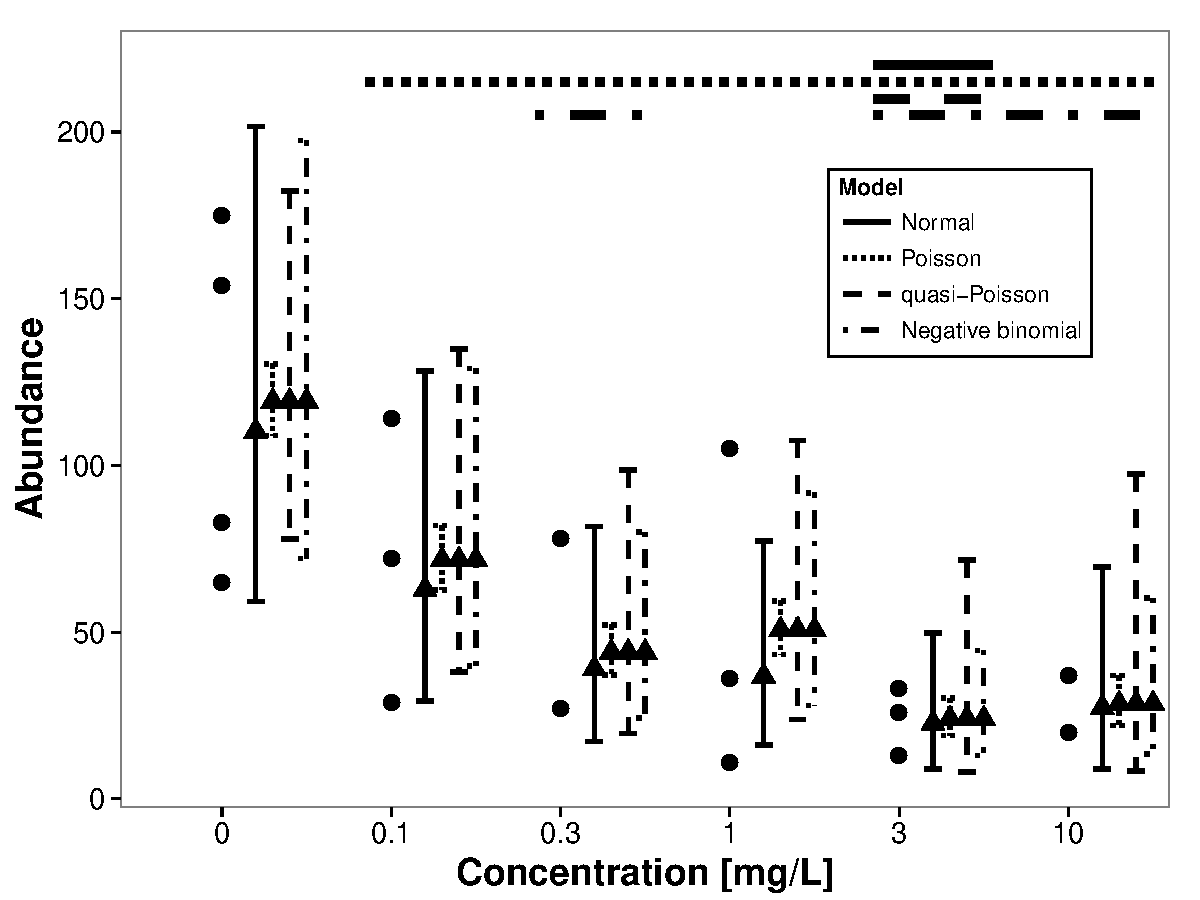
\includegraphics[width = 0.8\textwidth]{chapters/usetheglm/example.pdf}
  \caption[Example data from Brock et al. (2015).]{Data from \citet{brock_minimum_2015} (dots). 
  Predicted values (triangles) and 95\% Wald Z or t confidence intervals from the fitted models (vertical lines) are given beside.
  Horizontal bars above indicate treatments statistically significant different from the control group (Dunnett contrasts).
  The data showed considerable overdispersion ($\kappa = 3.91, \phi = 22.41$) and therefore, the Poisson model underestimates the width of confidence intervals.
  }
  \label{fig:usetheglm:example}
\end{figure}


%% --------------------------------
\subsection{Simulations}
\label{ssec:usetheglm:simulations}
\subsubsection{Count data}
To further scrutinise the differences between methods we simulated data sets with known properties.
We simulated count data that mimics the data of the case study with five treatments (T1 - T5) and one control group (C).
Counts were drawn from a negative binomial distribution with overdispersion at all treatments ($\kappa = 4$, eqn. \ref{eqn:usetheglm:negbin}).
We simulated data sets with different number of replicates (N = \{3, 6, 9\}) and different abundances in control treatments ($\mu_\text{\tiny C}$ = \{2, 4, 8, 16, 32, 64, 128\}). 
For Type I error estimation mean abundance was equal between treatments.
For power estimation, mean abundance in treatments T2 - T5 was reduced to half of control and T1 ($\mu_\text{\tiny T2}~=~...~=~\mu_\text{\tiny T5}~=~0.5~\mu_\text{\tiny C} = 0.5~\mu_\text{\tiny T1}$), resulting in a theoretical LOEC at T2.
We generated 1000 data sets for each combination of N and $\mu_\text{\tiny C}$ and analysed these using the models outlined in section \ref{ssec:usetheglm:counts}.


%% --------------------------------
\subsubsection{Binomial data}
We simulated data from a commonly used design as described in \citet{weber_short-term_1989}, with 5 treated (T1 - T5) and one control group (C). 
Proportions were drawn from a Bin(10, $\pi$) distribution, with varying probability of survival ($\pi$ = \{0.60, 0.65, 0.70, 0.75, 0.80, 0.85, 0.90, 0.95\}) and varying number of replicates (N = \{3, 6, 9\}).
For Type I error estimation, $\pi$ was equal between treatments.
For power estimation $\pi$ was fixed at 0.95  in C and T1 and varied only in treatments T2 - T5. 
For each combination we simulated 1000 data sets and analysed these using the models outlined in section \ref{ssec:usetheglm:bin}.


%% --------------------------------
\subsection{Data Analysis}
\label{ssec:usetheglm:analysis}
We analysed the case study and the simulated data using the outlined methods.
We compared the methods and models in terms of Type I error (detection of an effect when there is none) and power (ability to detect an effect when it is present) at a significance level of $\alpha = 0.05$.

All simulations were done in R (Version 3.1.2) \citep{r_core_team_r:_2014} on an Amazon EC2 virtual Linux server (64bit, 15GB RAM, 8 cores, 2.8 GHz).
Source code to reproduce the simulations and paper is available online at \url{https://github.com/EDiLD/usetheglm}.
Moreover, Supplement \ref{ap:usetheglm:examples} provides worked examples of the data of \citet{brock_minimum_2015} and \citet{weber_short-term_1989}.


%% ----------------------------------------------------------------------------
\section{Results}
\label{sec:usetheglm:results}
%% --------------------------------
\subsection{Case study}
The data set showed considerably higher variance then expected by the Poisson model ($\phi = 22.41$ (eqn. \ref{eqn:usetheglm:quasi}), $\kappa = 3.91$ (eqn. \ref{eqn:usetheglm:negbin})). 
Therefore, the Poisson model did not fit to this data and led to underestimated standard errors and confidence intervals, as well as overestimated statistical significance (Figure \ref{fig:usetheglm:example}).
In this case, inferences on the Poisson model are not valid and we do not further discuss its results.
The normal (F = 2.57, p = 0.084) and quasi-Poisson model (F = 2.90, p = 0.061), as well as the Kruskal test (p =  0.145) did not show a statistically significant treatment effects.
By contrast, the LR test and parametric bootstrap of the negative binomial model indicated a treatment-related effect (LR = 13.99, p = 0.016, bootstrap: p = 0.042).

All methods predicted similar values, except the normal model predicting always lower abundances (Figure \ref{fig:usetheglm:example}). 
95\%~confidence intervals (CI) were most narrow for the negative binomial model and widest for the quasi-Poisson model - especially at lower estimated abundances.
Consequently, the LOECs differed (Normal and quasi-Poisson: 3 mg/L, negative binomial: 0.3 mg/L).
The pairwise Wilcoxon test did not detect any treatment different from control.


%% --------------------------------
\subsection{Simulations}
\subsubsection{Count data}
For detecting a general treatment effect, $GLM_{nb}$ and $GLM_{p}$ showed inflated Type I error rates, whereas $KW$ was conservative at low sample sizes.
However, using the parametric bootstrap for the negative binomial model ($GLM_{npb}$), as well as $LM$ and $GLM_{qp}$ resulted in appropriate Type I error rates.
For detecting a treatment effect,$GLM_{qp}$ had the highest power, followed by $GLM_{npb}$, $LM$ and $KW$, the latter having least power (Figure \ref{fig:usetheglm:p_glob_c}).
For our simulation design (reduction in abundance by 50\%) a sample size per treatment of n = 9 was needed to achieve a power greater than 80\%.
At small sample sizes (n = {3, 6}) and low abundances ($\mu_C$ = {2, 4}) many of the negative binomial models ($GLM_{nb}$ and $GLM_{npb}$) did not converge to a solution (convergence rate \textless 85\% of the simulations, Supplement  \ref{ap:usetheglm:tables}). 

For LOEC determination $GLM_{nb}$ and $GLM_{p}$ showed an increased Type I error and all other methods were slightly conservative.
The inferences on LOEC generally showed less power.
$LM$ showed a mean reduction of 20.7\% and $GLM_{qp}$ of 24.3 \%.
Power to detect the LOEC was highest for $GLM_{qp}$. 
$LM$ and $WT$ showed less power, with $WT$ having no power to detect the LOEC at low sample sizes (Figure \ref{fig:usetheglm:p_loec_c}).


\subsubsection{Binomial data}
$GLM_{bin}$ showed slightly increased Type I error rates at low sample sizes and small effect sizes.
$KW$ was more conservative than $LM$ and $GLM_{bin}$.
In addition, $GLM_{bin}$ exhibited the greatest power for testing the treatment effect. 
This was especially apparent at low sample sizes (n = 3), with up to 27\% higher power compared to LM.
However, the differences between methods quickly vanished with increasing samples sizes (Figure \ref{fig:usetheglm:p_glob_p}).

For inference on LOEC we found that all methods were slightly conservative.
$WT$ was generally more conservative and $GLM_{bin}$ especially at low effect sizes ($p_E > 0.7$).
Inference on LOEC was not as powerful as inference on the general treatment effect.
Contrary to the general treatment effect, $LM$ showed the higher power than $GLM_{bin}$ at small sample sizes (n = {3, 6}).
$WT$ had no power for n = 3 and showed less power in the other simulation runs (Figure \ref{fig:usetheglm:p_loec_p}).

\begin{landscape}
\begin{figure}
  \centering
  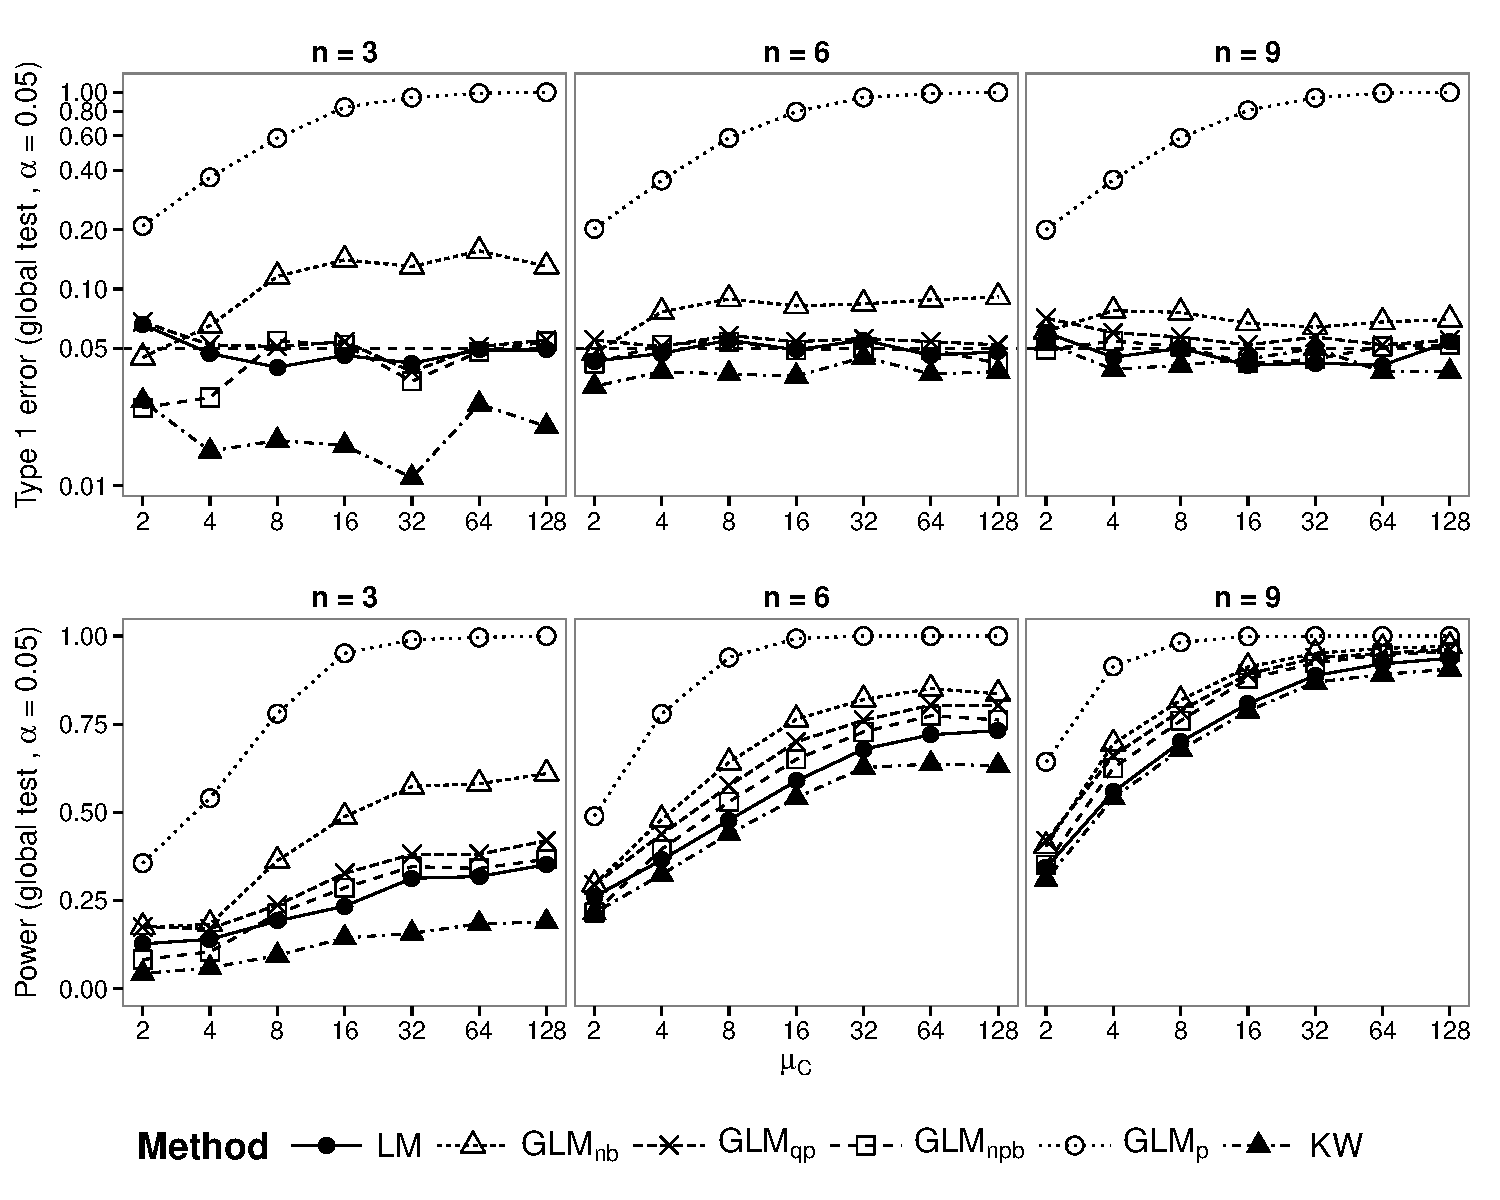
\includegraphics[width = 1.05\textwidth]{chapters/usetheglm/p_glob_c.pdf}
  \caption[Count data simulations: Type I error and Power for the test of a treatment effect.]{Count data simulations: Type I error (top) and Power (bottom) for the test of a treatment effect.
  Type I errors are displayed on a logarithmic scale.
  Power levels for models with inflated Type I errors ($GLM_P$ and $GLM_{qp}$) are shown for completeness. 
  For n = \{3, 6\} and $\mu_C$ = \{2, 4\} less than 85\% of $GLM_{nb}$ and $GLM_{npb}$ models did converge.
  Dashed horizontal line denotes the nominal I error rate at $\alpha = 0.05$.
  }
  \label{fig:usetheglm:p_glob_c}
\end{figure}
\end{landscape}


\begin{landscape}
\begin{figure}
  \centering
  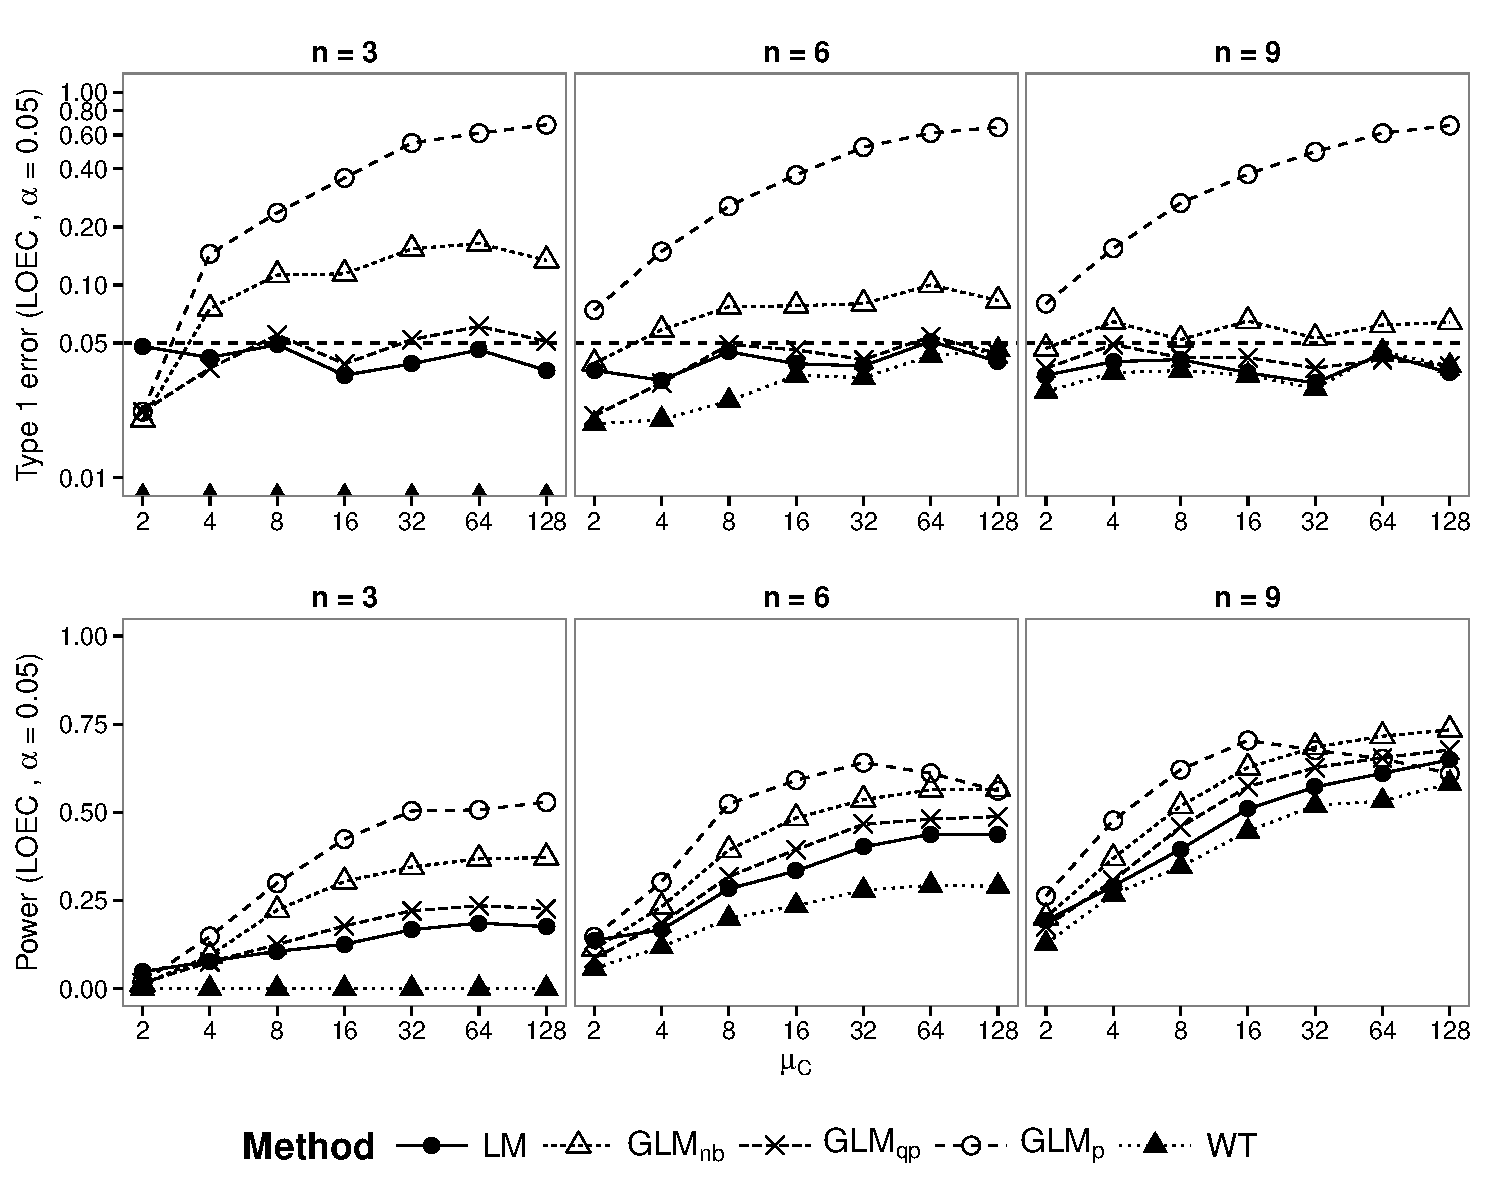
\includegraphics[width = 1.05\textwidth]{chapters/usetheglm/p_loec_c.pdf}
  \caption[Count data simulations: Type I error and Power for determination of LOEC.]{Count data simulations: Type I error (top) and Power (bottom) for determination of LOEC.
  Type I errors are displayed one a logarithmic scale.
  Power levels for models with inflated Type I error are shown for completeness.
  For n = \{3, 6\} and $\mu_C$ = \{2, 4\} less than 85\% of $GLM_{nb}$ models did converge.
  Dashed horizontal line denotes the nominal Type I error rate at $\alpha = 0.05$.
  }
  \label{fig:usetheglm:p_loec_c}
\end{figure}
\end{landscape}


\begin{landscape}
\begin{figure}
  \centering
  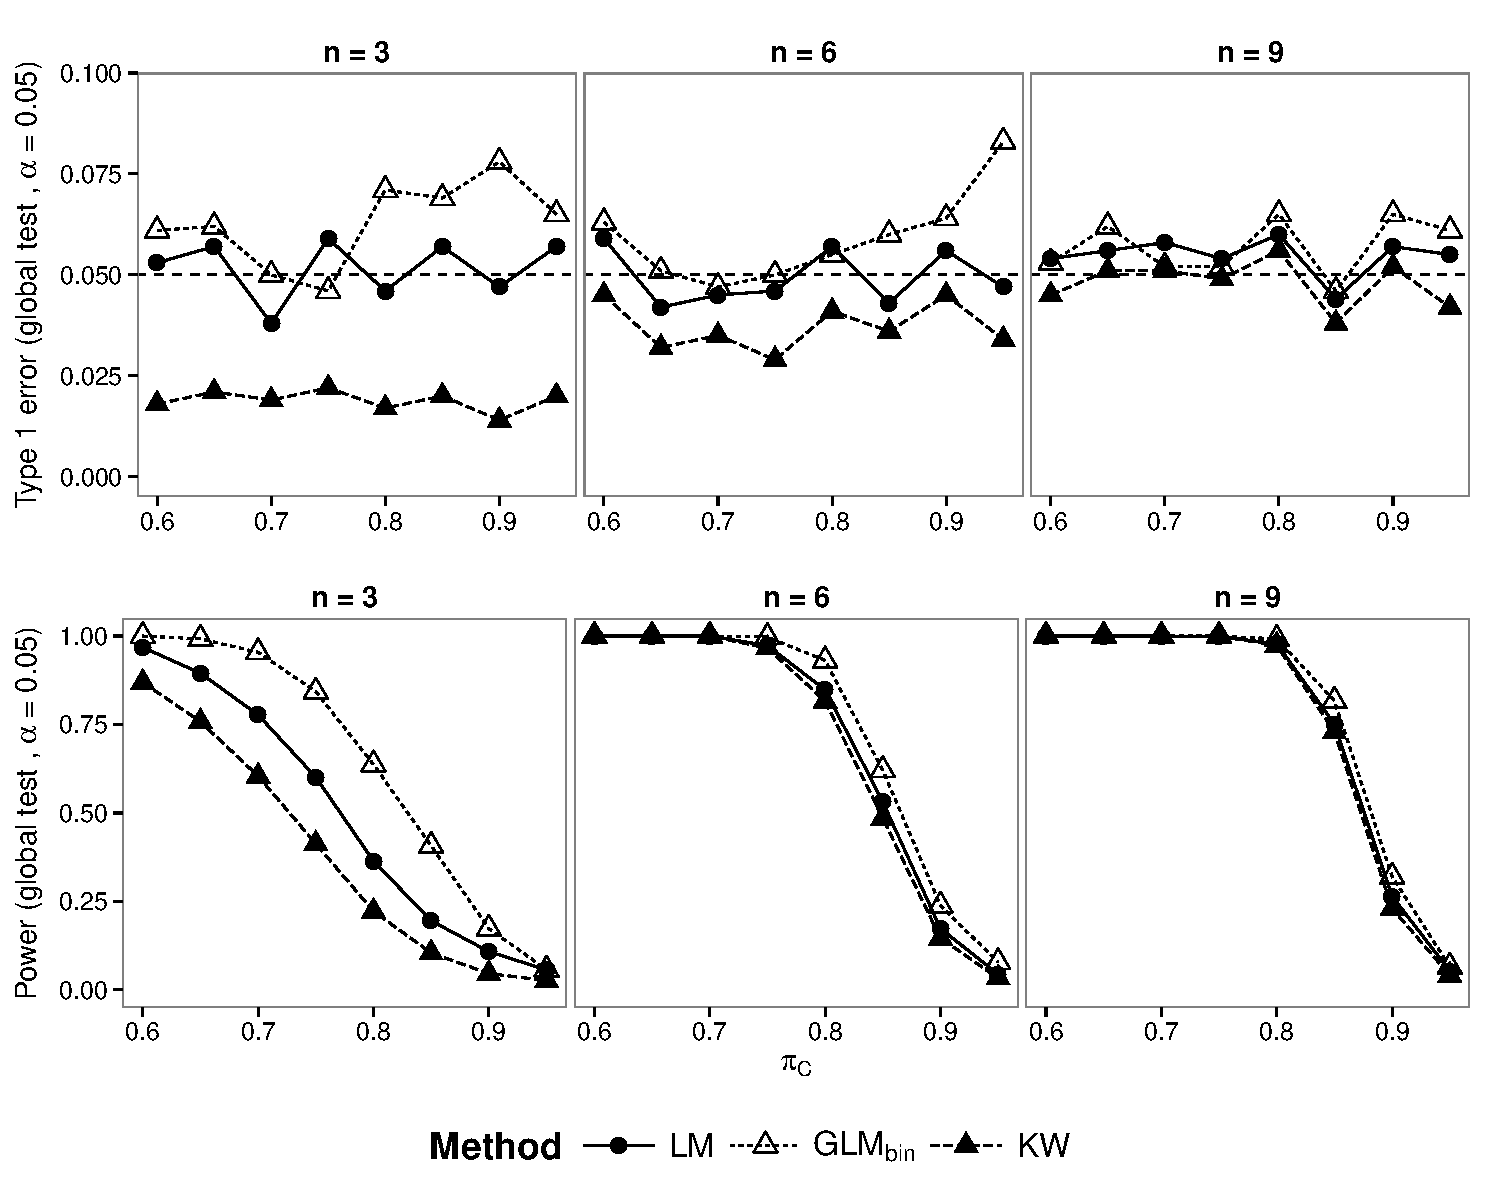
\includegraphics[width = 1.05\textwidth]{chapters/usetheglm/p_glob_p.pdf}
  \caption[Binomial data simulations: 
  Type I error and  power for the test of a treatment effect.]{
  Binomial data simulations: Type I error (top) and  power (bottom) for the test of a treatment effect. 
  Dashed horizontal line denotes the nominal Type I error rate at $\alpha = 0.05$.
  }
  \label{fig:usetheglm:p_glob_p}
\end{figure}
\end{landscape}

\begin{landscape}
\begin{figure}
  \centering
  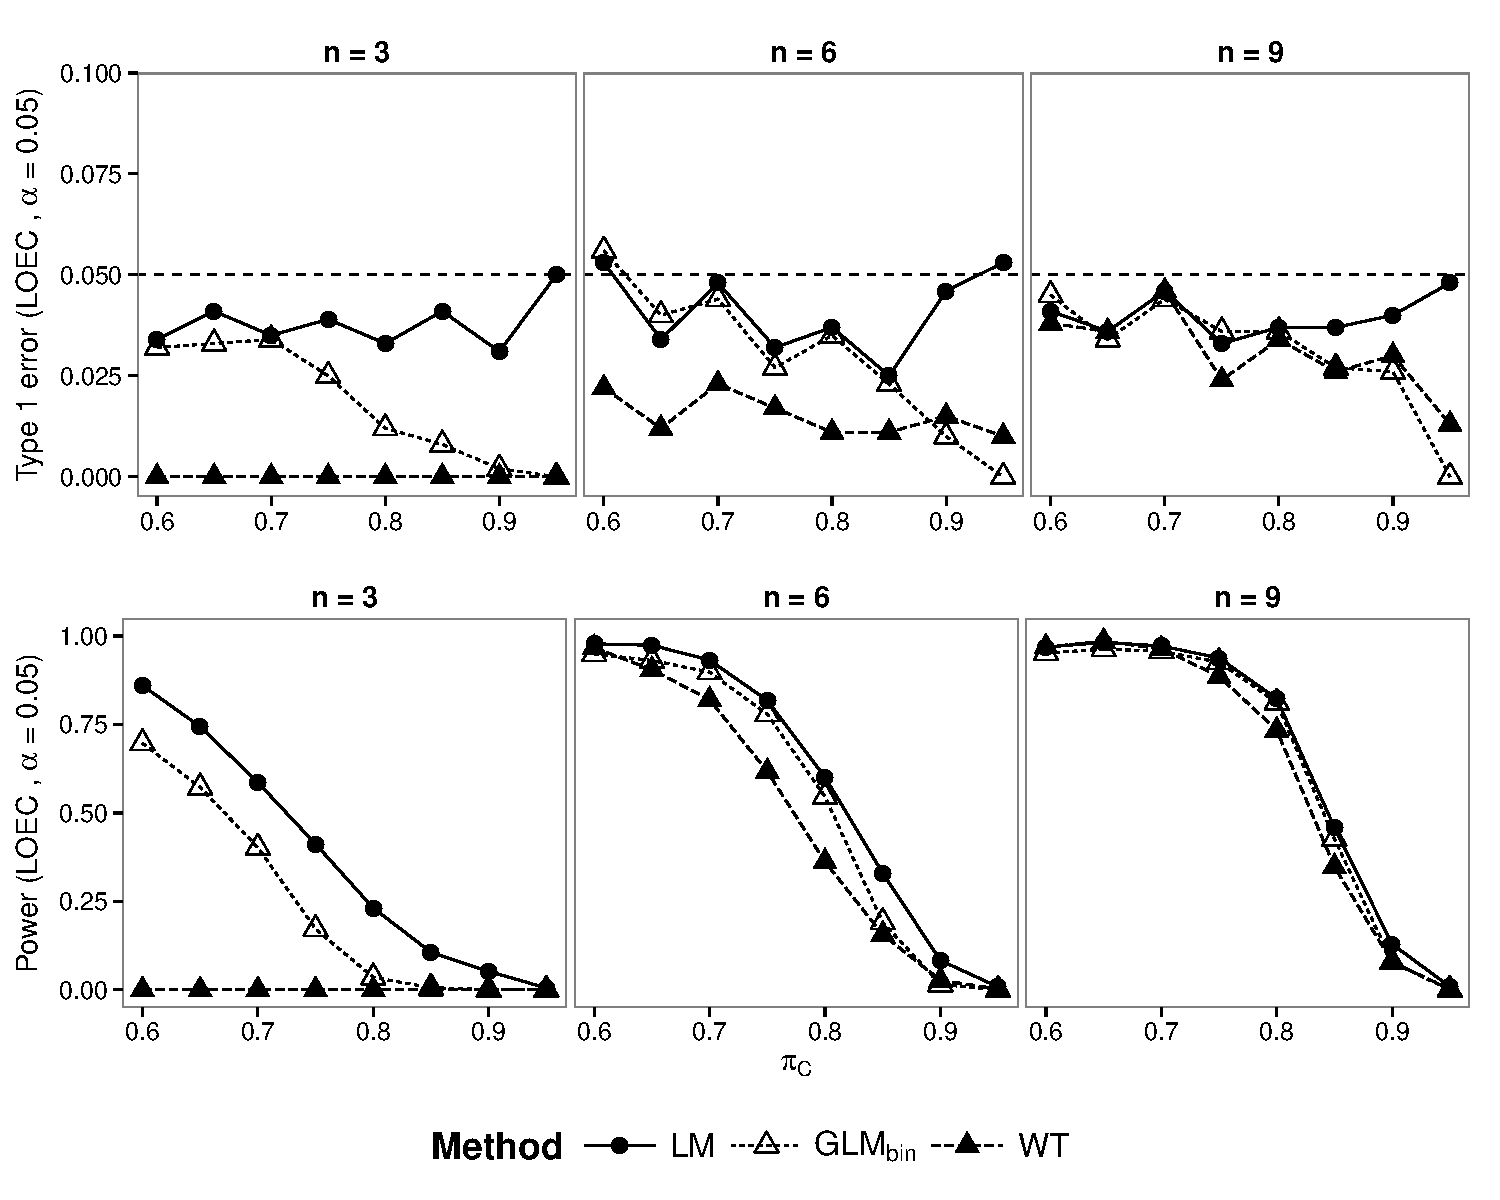
\includegraphics[width = 1.05\textwidth]{chapters/usetheglm/p_loec_p.pdf}
  \caption[Binomial data simulations: 
  Type I error and power for the test for determination of LOEC.]{
  Binomial data simulations: 
  Type I error (top) and power (bottom) for the test for determination of LOEC. 
  Dashed horizontal line denotes the nominal Type I error rate at $\alpha = 0.05$.
  }
  \label{fig:usetheglm:p_loec_p}
\end{figure}
\end{landscape}



%% ----------------------------------------------------------------------------
\section{Discussion}
\label{sec:usetheglm:disc}
\subsection{Case study}
%% ---- Case study
The outlined case study demonstrates that the choice of the statistical model and procedure can have substantial impact on ecotoxicological inferences and endpoints like the LOEC.
Therefore, ecotoxicologists should not base their inferences solely on statistical significance tests, but also on model estimates, their uncertainty and importance \citep{gelman_difference_2006}.
\citet{ohara_not_2010} showed that the linear model on log transformed data gave unreliable and biased estimates, whereas GLMs performed well with little bias.
Bias occurs also when back-transforming fitted means to the original scale, which explains the lower predicted means by $LM$ in Figure \ref{fig:usetheglm:example} \citep{rothery_cautionary_1988} and should be corrected for \citep{newman_regression_1993}.
When applied to non-transformed data, the linear model would predict identical treatment means as GLMs, because for a categorical predictor the predicted means of the LM and GLM are identical. 
When applied to non-transformed data, the linear model would result in identical predicted treatment means as GLMs. 
However, predictions would differ with continuous predictors and GLMs are particularly advantageous in this case.

This is further highlighted by the fact that for the same model (linear model applied to transformed data), \citet{brock_minimum_2015} reported a 10-fold lower LOEC (\mbox{0.3 mg/L}) then found in our study (3 mg/L, Figure \ref{fig:usetheglm:example}).
The reasons are manifold: 
(i)~\citet{brock_minimum_2015} used a $log(2~y + 1)$ transformation, whereas we used a $log(A~y + 1)$ transformation, where A = 2 / 11 = 0.182 \citep{van_den_brink_impact_2000}.
(ii)~We adjusted for multiple testing using Holm's (\citeyear{holm_simple_1979}) method.
(iii)~\citet{brock_minimum_2015} used a one-sided Williams test \citep{williams_comparison_1972}, whereas we used one-sided comparisons to the control (Dunnett contrasts).
The choice of transformation contributed only little to the differences. 
If the assumptions of Williams test  are met it has strictly greater power than Dunnett contrasts \citep{jaki_statistical_2013}, which explains the differences in the case study.
A generalisation of the Williams test as multiple contrast test (MCT) can be used in a GLM framework \citep{hothorn_simultaneous_2008}.
Nevertheless, such a Williams-type MCT is not a panacea \citep{hothorn_statistical_2014} and our simulated semi-concave dose-response relationship is a situation where it fails and likely underestimates the LOEC \citep{kuiper_identification_2014}. 
 

%% ---- Guide GLMs
Overdispersion is common for ecological datasets \citep{warton_many_2005} and the case study illustrates the potential effects of overdispersion that is not accounted for: standard errors will be underestimated and significance overestimated (Figures \ref{fig:usetheglm:example}).
This is also shown by our simulations (Figures \ref{fig:usetheglm:p_glob_c}, \ref{fig:usetheglm:p_loec_c}) where $GLM_p$ showed increased Type I error rates because of overdispersed simulated data. 
However, in factorial designs the mean-variance relationship can be easily \newline 
checked by plotting mean versus variance of the treatment groups or by inspecting residual versus fitted values plots (see Supplement \ref{ap:usetheglm:examples}).
Our simulations revealed that the LR test for $GLM_{nb}$ is invalid because of increased Type I errors. This explains why it had the lowest p-value in the case study.

In the introduction we pointed out that there is little advice how to choose between the plenty of possible transformations - how do GLMs simplify this problem?
The distribution modeled can be chosen using knowledge about the data (e.g. bounds, integer or continuous data etc).
Knowing what type of data is modeled (see Methods section), the model selection process can be completely guided by the data and diagnostic tools. Therefore, choosing an appropriate model is easier than choosing between possible transformations.


\subsection{Simulations}
\label{ssec:usetheglm:discsim}
%% --- general low power
Our simulations showed that GLMs have generally greater power than the linear model applied to transformed data.
However, the simulations also suggest that the power at the population level in common mesocosm experiments is low.
For common samples sizes ($n \le 4$ ) and a reduction in abundance of 50\% we found a low power to detect any treatment-related effect (\textless 50\% for methods with appropriate Type I error, Figure \ref{fig:usetheglm:p_glob_c}).
Statistical power to detect the correct LOEC was even lower (less than 25\%), which can be attributed to multiple testing.
The low power of all methods to detect significant treatment levels such as the LOEC or NOEC suggests that these endpoints from ecotoxicological studies should be interpreted with caution and underpins their criticism \citep{laskowski_good_1995,landis_well_2011}.

%% --- Multivariate + GLMM -------
Mesocosm studies allow also for inferences on the community level. 
For community analyses \emph{GLM for multivariate data} \citep{warton_distance-based_2012} have been proposed as alternative to Principal Response Curves (PRC) and yielded similar inferences, but better indication of responsive taxa \citep{szocs_analysing_2015}. 
However, \citet{ter_braak_topics_2014} argue to use data transformations with community data because of their simplicity and robustness.
Although our simulations covered only simple experimental designs at the population level, findings may also extend to more complex situations. 
Nested or repeated designs with non-normal data could be analysed using Generalised Linear Mixed Models (GLMM) and may have advantages with respect to power \citep{stroup_rethinking_2014}.

%% --- Alternatives -------
To counteract the problems with low power at the population level \citet{brock_minimum_2015} proposed to take the Minimum Detectable Difference (MDD), a method to assess statistical power \emph{a posteriori}, for inference into account.
However, \emph{a priori} power analyses can be performed easily using simulations, even for complex experimental designs \citep{johnson_power_2015}, and might help to design, interpret and evaluate ecotoxicological studies.
Moreover, \citet{brock_minimum_2015} proposed that statistical power of mesocosm experiments can be increased by reducing sampling variability through improved sampling techniques and quantification methods, though they also caution against depleting populations through more exhaustive sampling.
As we showed, using GLMs can enhance the power at no extra costs.

%% --- Non-parametric
\citet{wang_making_2011} advocated that in the typical case of small sample sizes (n \textless20) and non-normal data, non-parametric tests perform better than parametric tests assuming normality.
In contrast, our results showed that the often applied $KW$ and $WT$ have less power compared to $LM$.
Moreover, $GLMs$ always performed better than non-parametric tests. 
Though more powerful non-parametric tests may be available \citep{konietschke_rank-based_2012}, these are focused on hypothesis testing and do not provide estimation of effect sizes.
Additionally to testing, GLMs allow the estimation and interpretation of effects that might not be statistically significant, but ecologically relevant.
Therefore, we advise using GLMs instead of non-parametric tests for non-normal data.

%% ---- Problems GLM
We found an increased Type-I error for $GLM_{nb}$ at low sample sizes.
However, it is well known that the LR statistic is not reliable at small sample sizes \citep{bolker_generalized_2009,wilks_large-sample_1938}.
Parametric bootstrap ($GLM_{npb}$) is a valuable alternative in such situations and maintains appropriate levels (Figure \ref{fig:usetheglm:p_glob_c}).
Moreover, at small sample sizes and low abundances a significant amount of negative binomial models did not converge.
We used an iterative algorithm to fit these models \citep{venables_modern_2002} and other methods assessing the likelihood directly may perform better.

$GLM_{qp}$ showed higher statistical power than $GLM_{npb}$ (Figure \ref{fig:usetheglm:p_glob_c}, bottom).
This could be explained by the simpler mean-variance relationship of $GLM_{qp}$ (eqn. \ref{eqn:usetheglm:quasi} and \ref{eqn:usetheglm:negbin}), because at small samples sizes, low abundances or few treatment groups it is difficult to determine the mean-variance relationship.
Our results are similar to \citet{ives_for_2015}, who compared GLMs to LM applied to transformed data for testing regression coefficients.
Because of inflated Type I errors for $GLM_{nb}$ and, in the case of multiple explanatory variables in the model, inflated Type I errors of $GLM_{qp}$ he considered the LM on transformed data as most robust and recommended its preferred use.
However, we showed that the parametric bootstrap LR test of $GLM_{nb}$ provides appropriate Type I errors and bootstrapping might be an alternative for testing coefficients.
Nevertheless, bootstrapping is computationally very intensive and we found no gains in power compared to $GLM_{qp}$ (Figure \ref{fig:usetheglm:p_glob_c}). 
Given the higher power, appropriate Type I errors, stable convergence and reduced bias \citep{ohara_not_2010} we suggest that count data in one factorial experiments should be analysed using the quasi-Poisson model.


%% --- binomial data
Binomial data are often collected in lab trials, where increasing the sample size may be relatively easy to accomplish. 
We found notable differences in power to detect a treatment effect for all simulated sample sizes.
Similarly, \citet{warton_arcsine_2011} also found that GLMs have higher power than arcsine transformed linear models.
Though we did not simulate overdispersed binomial data, this should be checked and accounted for.
In such situations a GLMM may offer an appealing alternative \citep{warton_arcsine_2011}.
At low effect sizes $GLM_{bin}$ became conservative with increasing $\pi_C$, although this effect lessened as sample size increased (Figure \ref{fig:usetheglm:p_loec_p}). 
This is because $\pi$ approaches its boundary and is also known as the \emph{Hauck-Donner effect} \citep{hauck_walds_1977}. A LR-Test or parametric bootstrap may provide an alternative in such situations \citep{bolker_generalized_2009}.
This can also explain why $LM$ performed better for deriving LOECs at low sample sizes.

\clearpage
GLMs can be fitted with several statistical software packages and many textbooks are available to introduce ecotoxicologists to these models (e.g. \citealt{zuur_beginners_2013} or \citealt{quinn_experimental_2009}).
We recommend that ecotoxicologists should change their models instead of their data.
GLMs should become a standard method in ecotoxicology and incorporated into respective guidelines.

%% ----------------------------------------------------------------------------
\clearpage
\section{References}
\printbibliography[heading=none]


%---------------------------------------------n-------------------------------
% Pesticides Small streams
\cleardoublepage
\def\dir{chapters/smallstreams}
% -*- root: ../../thesis.tex -*-

\chapter{Large scale risks from pesticides in small streams}
\label{sec:smallstreams}  

\begin{sloppypar}
\bigskip
\underline{Eduard Szöcs\textsuperscript{a}}, Marvin Brinke\textsuperscript{b}, Bilgin Karaoglan\textsuperscript{c} \& Ralf B. Schäfer\textsuperscript{a}

\bigskip
\small
\noindent 
\textsuperscript{a}Institute for Environmental Sciences, University Koblenz-Landau, Landau, Germany \\
\textsuperscript{b}German Federal Institute of Hydrology (BfG), Koblenz, Germany \\
\textsuperscript{c}German Environment Agency (UBA), Dessau-Roßlau, Germany

\bigskip 
\normalsize
\noindent
Submitted to \emph{Environmental Science \& Technology} in 2016

\end{sloppypar}
\newpage


%% ----------------------------------------------------------------------------
\section{Abstract}
Small streams are important refugia for biodiversity.
In agricultural areas they may be at high risk from pesticide pollution. 
However, most related studies have been limited to a few streams on the regional level, hampering extrapolation to larger scales. 
We used data from German governmental water quality monitoring to quantify the drivers of pesticide risk and to assess pesticide risk in small streams on a large scale. 
The data set comprised of 1,766,104 measurements of 478 pesticides (including metabolites) related to 24,743 samples from 2,301 sampling sites. 
We investigated the influence of agricultural land use, catchment size, as well as precipitation and seasonal dynamics on pesticide risk using new statistical modelling techniques that explicitly consider the limit of quantification. 
Agricultural land use lead to a 3.7-fold increase in exceedance of risk thresholds when the proportion of agriculture in a catchment exceeded 28 percent. 
Precipitation increased pesticide risk by 36\% and risk was the highest during summer months. 
Risk thresholds were exceeded in 26\% of streams, with the highest risk related to neonicotinoid insecticides. 
We conclude that pesticides from agricultural land use are a major threat to small streams and their biodiversity and that a realistic pesticide sampling would be driven by precipitation events. 

%% -------------------------------------------------------------------------
\section{Introduction}
More than 50\% of the total land area in Germany is used by agriculture \citep{statistisches_bundesamt_bodenflache_2014}.
In the year 2014 more than 45,000 tonnes of 776 authorised plant protection products were sold for application on this area \citep{bundesamt_fur_verbraucherschutz_und_lebensmittelsicherheit_absatz_2015}.
The applied pesticides may enter surface waters via spray-drift, edge-of-field run-off or drainage \citep{stehle_probabilistic_2013,schulz_comparison_2001,liess_determination_1999}.
Once entered the surface waters they may have adverse effects on biota and ecosystem functioning \citep{schafer_thresholds_2012}. 
Although it is known that pesticide pollution and its ecological effects increase with the fraction of agricultural land use in the catchment \citep{schulz_field_2004}, the shape of the relationship is unknown and studies on potential thresholds are lacking.

Two recent studies indicate that pesticides might threaten freshwater biodiversity in the European union.
\citet{malaj_organic_2014} analysed data supplied to the European Union (EU) in the context of the Water Framework Directive (WFD) and showed that almost half of European water bodies are at risk from pesticides.
\citet{stehle_pesticide_2015} compiled 1,566 measured concentrations of 23 insecticides in the EU from scientific publications. 
They found that many of these measurements exceed regulatory acceptable concentrations (RAC).
However, these studies reflect only a small amount of potentially available data (173 sites in predominantly mid-sized and large rivers in \citet{malaj_organic_2014} and 138 measurements in \citet{stehle_pesticide_2015}), and it is unclear how representative they are for Germany. % 173 estimated from digitized figure C.3 in Malaj 2014; Stehle: Table 2.
Much more comprehensive data on thousands of sites are available from national monitoring programs that are setup for the surveillance of water quality,
which is done independently by the federal states in Germany in compliance with the WFD \citep{quevauviller_water_2008} and additional state-specific needs. 
Despite that these data are providing the opportunity to study pesticide risks and other research questions on a large scale with high spatial density, to date these data have not been compiled and related analyses are lacking. 

Small streams comprise a major fraction of streams \citep{nadeau_hydrological_2007}, accommodate a higher proportion of biodiversity compared to larger freshwater systems \citep{davies_comparison_2008, biggs_report_2014} and play an important role in the recolonization of disturbed downstream reaches \citep{liess_analyzing_2005, orlinskiy_forested_2015}.
Nevertheless, a clear definition of small streams in terms of catchment or stream size is currently lacking \citep{lorenz_specifics_2016}. 
For example, the WFD defines small streams with a catchment size between 10 and 100 km\textsuperscript{2}, without further categorisation of streams \textless 10km\textsuperscript{2} and \citet{lorenz_specifics_2016} defines small streams with catchment size \textless 10km\textsuperscript{2}. 
Moreover, small streams might particularly be at high risk of pesticide contamination in case of adjacent agricultural areas given their low dilution potential \citep{schulz_field_2004,liess_determination_1999}.
Indeed, meta-analyses using data from studies with a few sites reported higher pesticide pollution in smaller streams compared to bigger streams \citep{stehle_pesticide_2015,schulz_field_2004}. 
Despite their ecological relevance and potentially higher pesticide exposure, a recent analysis of pesticide studies showed that a disproportionally small fraction of studies was conducted in small water bodies, and these were largely limited to a few sites \citep{lorenz_specifics_2016}. 
Consequently, knowledge on the pesticide pollution of small streams on larger scales is scant. 
In European law, the Directive 2009/128/EC \citep{European_Union_2009} places an obligation on the EU Member States to adopt National Action Plans (NAP) for the Sustainable Use of Plant Protection Products and the German NAP also addresses the knowledge gap concerning pesticide impact on small streams, specifically including those with catchment size \textless 10km\textsuperscript{2}.

In this study, we compiled and analysed large-scale chemical monitoring data from small streams in Germany. 
First, we analysed the shape of the relationship between pesticide risk, agricultural land use, and catchment size and examined whether related thresholds for pesticide risks can be derived. 
Second, we investigated the influence of precipitation and seasonal dynamics on pesticide detections, given that precipitation proved an important driver of pesticide exposure in several small-scale studies \citep{wittmer_significance_2010,schulz_field_2004}, but it is unknown whether a precipitation signal prevails on large scales. 
Finally, we quantified the current risks from pesticides in small streams in Germany and the compounds accountable for the risk.



%% -------------------------------------------------------------------------
\section{Methods}
\subsection{Data compilation}
We queried pesticide monitoring data from sampling sites that can be classified as small streams (catchment sizes $\mathrm{< 100~km^2}$ according to the WFD) from all 13 non-city federal states of Germany (see Supplemental Table~S1 for the abbreviations of federal state names) for 2005 to 2015.
We homogenised and unified all data provided by the federal states into a database and implemented a robust data-cleaning workflow (see Supplemental Figure~S1 for details) \citep{poisot_best_2015}.

We identified precipitation at sampling sites by a spatio-temporal intersection of sampling events with gridded daily precipitation data (60$\times$30 arcsec resolution) available from the German Meteorological Service (DWD).
This data spatially interpolates daily precipitation values from local weather stations \citep{rauthe_central_2013}. 
We performed the intersection for the actual sampling date and the day before and extracted precipitation during and up to 48 hours before sampling. 


\subsection{Characterization of catchments}
We compiled a total of 2,369 sampling sites in small streams with pesticide measurements. %see do_overview.R
Alongside, we also queried catchment sizes and agricultural land use within the catchment for the sampling sites from the federal states. %see do_overview.R
Catchment size was provided for 59\% of sites. 
Additionally, we delineated upstream catchments for each of the sampling sites using (i) a digital elevation model (DEM) \citep{eea_digital_2013} and the multiple flow direction algorithm \citep{holmgren_multiple_1994} as implemented in GRASS GIS 7 \citep{neteler_grass_2012} and (ii) from drainage basins provided by the Federal Institute of Hydrology (BfG). 
Delineated catchments were visually checked for accuracy by comparison with state stream networks and derived information amalgamated with existing data.
Thus, catchment size information was available for 99\% of all sites (59\% from authorities, 24\% from DEM and 16\% from drainage basins). 

For each derived catchment (either from DEM or drainage basins) we calculated the \% agricultural land-use within the catchment based on the Authoritative Topographic-Cartographic Information System (ATKIS) of the land survey authorities \citep{adv_atkis_2016}. 
Thus, agricultural land use information was available for 98\% of all sites (24\% from authorities, 52\% from DEM and 22\% from drainage basins). 
68 sites (3\%) that lacked catchment size or land use information were omitted from the analysis, resulting in 2301 sites used in the analyses outlined below.
%see do_overview.R 



\subsection{Characterization of pesticide pollution}
We characterised pesticide pollution using regulatory acceptable concentrations (RAC) \citep{brock_linking_2010}.
RACs are derived during pesticide authorisation as part of the ecological risk assessment.
No unacceptable ecological effects are expected if the environmental concentration remains below this concentration.
\citet{stehle_pesticide_2015} showed that RAC exceedances reflect a decrease in biodiversity and from this perspective are ecologically relevant indicators. 
The German Environment Agency (UBA) provided RACs for 107 compounds, including those with the highest detection rates (Supplemental Table~S2). 
Based on theses RACs, we calculated Risk Quotients (RQ):

\begin{equation}
RQ_i = \frac{C_i}{RAC_i}
\end{equation}

where $C_i$ is the concentration of a compound $i$ in a sample and $RAC_i$ the respective RAC.


\subsection{Statistical analyses}
All data-processing and analyses were performed using R \citep{r_core_team_r:_2016}.
To display differences in the spectra of analysed compounds between federal states we used Multidimensional Scaling (MDS) based on Jaccard dissimilarity in conjunction with complete linkage hierarchical clustering using the vegan package \citep{oksanen_vegan:_2016}.
We determined the optimum number of clusters using the average silhouette width \citep{rousseeuw1987silhouettes}. 

We expected non-linear responses to agriculture and catchment size and therefore, used generalised additive models (GAM) to establish relationships \citep{fewster_analysis_2000}.
We modelled the number of RAC exceedances (RQ \textgreater 1) at a site as:

\begin{align}
\begin{split}
  No(RQ > 1)_i \sim NB(\mu_i, \kappa) \\
  log(\mu_i)= \beta_0 + f_1(agri_i) + f_2(size_i) + log(n_i) \\
\end{split}
\end{align}

where $No(RQ > 1)_i$ is the observed number of RAC exceedances at site $i$. 
We modelled $No(RQ > 1)_i$ as resulting from a negative binomial distribution ($NB$) with mean $\mu_i$ and a quadratic mean-variance-relationship ($Var(No(RQ > 1)_i) = \mu_i + \frac{\mu_i^2}{\kappa}$).
The proportion of agriculture within the catchment ($agri_i$) and the catchment size of the site ($size_i$) were used as predictors of the number of RAC exceedances. 
$\beta_0$ is the intercept and $f_1$ and $f_2$ are smoothing functions using penalized cubic regression splines \citep{wood_generalized_2006}. 
The degree of smoothness was estimated using restricted maximum likelihood (REML) during the model fitting process \citep{wood_fast_2011}.
The number of measurements per site ($n_i$) was used as an offset to account for differences in sampling efforts (sampling interval and analysed compound spectrum) at a site and is equivalent to modelling the rate of exceedances. 
We used point-wise 95\% Confidence Intervals (CI) of the first derivative of the fitted smooth to identify regions of statistically significant changes.
GAMs were fitted using the mgcv package \citep{wood_fast_2011}.

To assess the influence of precipitation and seasonality, we modelled the RQ of individual compounds as the response variable.
RQ and concentrations show a skewed distribution with an excess of zeros (no pesticides detected and quantified). 
Therefore, we modelled these as two processes (one generating values below the limit of quantification (LOQ) and one generating values above LOQ) using a Zero-Adjusted Gamma (ZAGA) distribution \citep{rigby_generalized_2005,stasinopoulos_gamlss.dist:_2016} (Equation~\ref{eqn:eqn3}).
These two processes can be interpreted as changes in the mean value of RQ (change in $\mu$) and changes in the probability of exceeding LOQ and showing any risk (change in $\nu$).

\begin{align}
RQ_i \sim ZAGA(\mu_i, \sigma, \nu_i) = 
  \begin{cases}
    (1 - \nu_i)   & \quad  \text{if } y < LOQ \\
    \nu_i \times f_{Gamma} (\mu_i, \sigma) & \quad \text{if } y \ge LOQ \\
  \end{cases}
  \label{eqn:eqn3}
\end{align}

$\nu_i$ denotes the probability of a measurement i being above LOQ and $f_{Gamma}$ denotes the gamma function and is used for values equal to or greater LOQ, with $\mu$ being the mean and $\sigma$ the standard deviation of RQ.
We used the $log(x+0.05)$ transformed precipitation at sampling date ($log~prec_0$) and the day before ($log~prec_{-1}$), as well as quarters of the year ($Q1-Q4$) as linear predictors for $\mu$ and $\nu$. 
We used appropriate link functions for $\mu$ and $\nu$ and assumed $\sigma$ to be constant. 
Equation~\ref{eqn:eqn4} summarises the deterministic part of the model for a measurement $i$.

\begin{align}
\begin{split}
\log(\mu_{i}) = log~prec_{0 i} + log~prec_{-1 i} + Q1_{i} + Q2_{i}+Q3_{i}+Q4_{i}\\
logit(\nu_{i}) = log~prec_{0 i} + log~prec_{-1 i} + Q1_{i} + Q2_{i}+Q3_{i}+Q4_{i}
\end{split}
\label{eqn:eqn4}
\end{align}

To account for temporal autocorrelation and differences between federal states we used $site$ nested within $state$ as random intercepts.
We implemented this model using the gamlss package \citep{stasinopoulos_generalized_2007}. 

We fitted this model separately to each compound with a RAC, measured in at least 1000 samples and with more than 5\% of values above LOQ (n = 22 compounds, see Supplemental Table~S3 for a list of compounds). 
To summarise the coefficients across the 22 modelled compounds we used a random effect meta-analysis for each model coefficient separately \citep{harrison_getting_2011}, resulting in an averaged effect of the 22 compounds.
The results of individual compounds are provided in the Supplemental Table~S4 and Figure~S7.
The meta-analysis was performed using the metafor package \citep{Viechtbauer_2010}. 



%% -------------------------------------------------------------------------
\section{Results}
\subsection{Overview of the compiled data}

The compiled dataset used for analysis comprised 1,766,104 pesticide measurements in 24,743 samples from 2,301 sampling sites in small streams.  %see do_overview.R for numbers.
These samples were all taken via grab sampling.  
We found large differences between federal states in the number of sampling sites and their spatial distribution (Figure~\ref{fig:ss:fig1} and Supplemental Table~S1). 
The number of small stream sampling sites per state ranged from 1 (Lower Saxonia, NI) to 1139 (North Rhine-Westphalia, NW).
No data were available from Brandenburg. 

\begin{figure}[ht]
  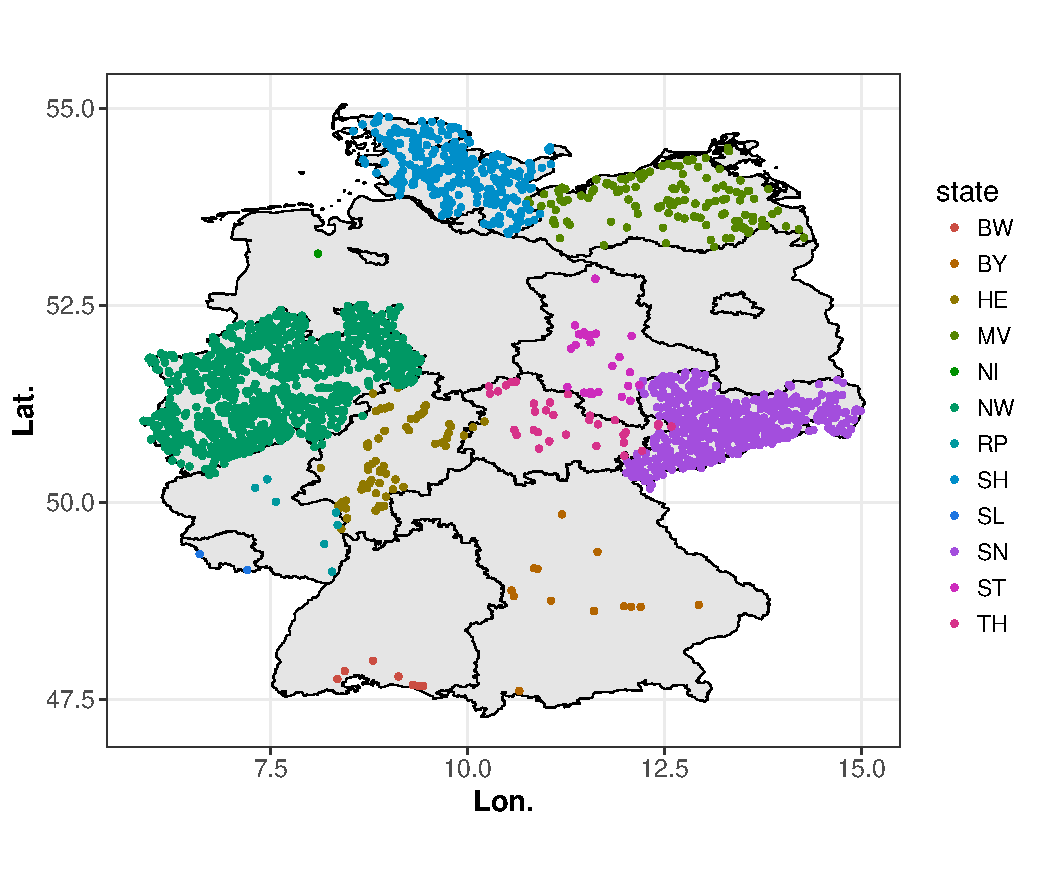
\includegraphics[width=1\textwidth]{chapters/smallstreams/figure1.pdf}
  \caption[Spatial distribution of the 2,301 small stream sampling sites.]{Spatial distribution of the 2,301 small stream sampling sites. Colour codes different federal states (see Supplemental Table~S1 for abbreviations).}
  \label{fig:ss:fig1}
\end{figure}

In total 478 different compounds used as pesticides and their metabolites were measured at least once (Supplemental Table~S2). 
Most of the compounds were herbicides (179), followed by insecticides (117) and fungicides (109). % see overview.R
Most samples were taken in the months April till October, while fewer samples were taken during winter (see Supplemental Figure~S2).
We found substantial differences in the spectra of analysed pesticides between federal states (Figure~\ref{fig:ss:fig2}).
The number of different pesticides per state ranged from 57 (SL) to 236 (RP) (Supplemental Table~S1). 
Hierarchical clustering revealed that RP and NI analysed distinct compound spectra compared to the cluster of other states. 
However, it has to be noted that both states surveyed these distinct spectra in special monitoring programs from only a few sites. 
Although there was high variability within the remaining cluster, this could not be further split (Figure~\ref{fig:ss:fig2}, also Supplemental Figures~S3 and S4).
4\% (=71,113) of all measurements were concentrations above LOQ.

\begin{landscape}
\begin{figure}[ht]
  \centering
  \vspace{1cm}
  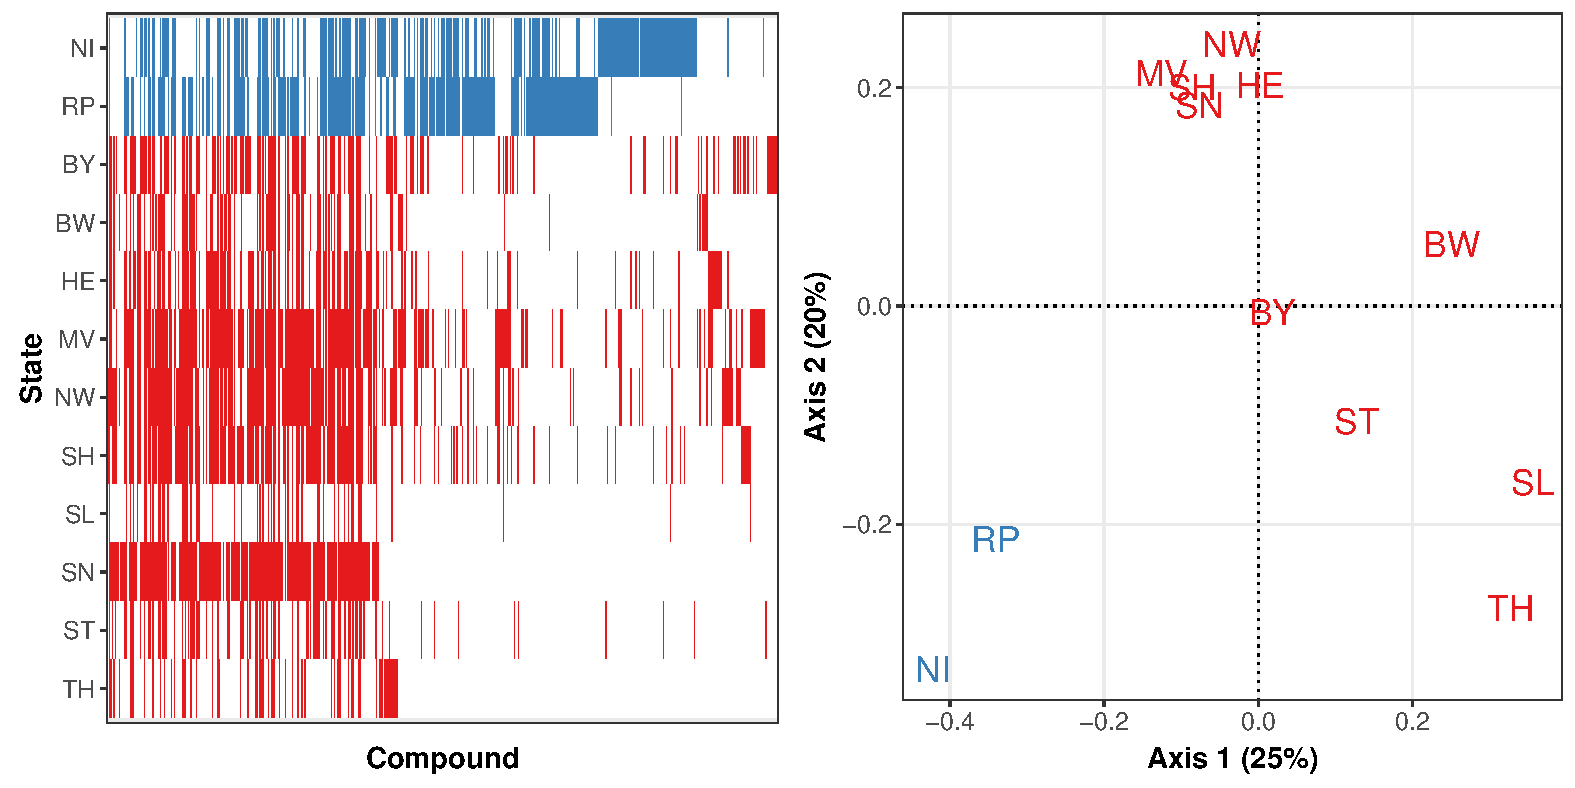
\includegraphics[width=0.8\textheight]{chapters/smallstreams/figure2.pdf}
  \caption[Compound spectra of the different federal states.]{Compound spectra of the different federal states. Left: Barcode plot - each vertical line is an analysed compound. Right: MDS ordination. 
  Colors according to two clusters determined by hierarchical clustering (see Supplemental Figure~S3 and S4).}
  \label{fig:ss:fig2}
\end{figure}
\end{landscape}


The distribution of sampling sites across catchment sizes indicated a disproportionally low number of sites with catchments below $10~km^2$, with
most sampling sites having catchment sizes between 10 and 25~$km^2$ (Figure~\ref{fig:ss:fig3}). 


\begin{figure}[ht]
  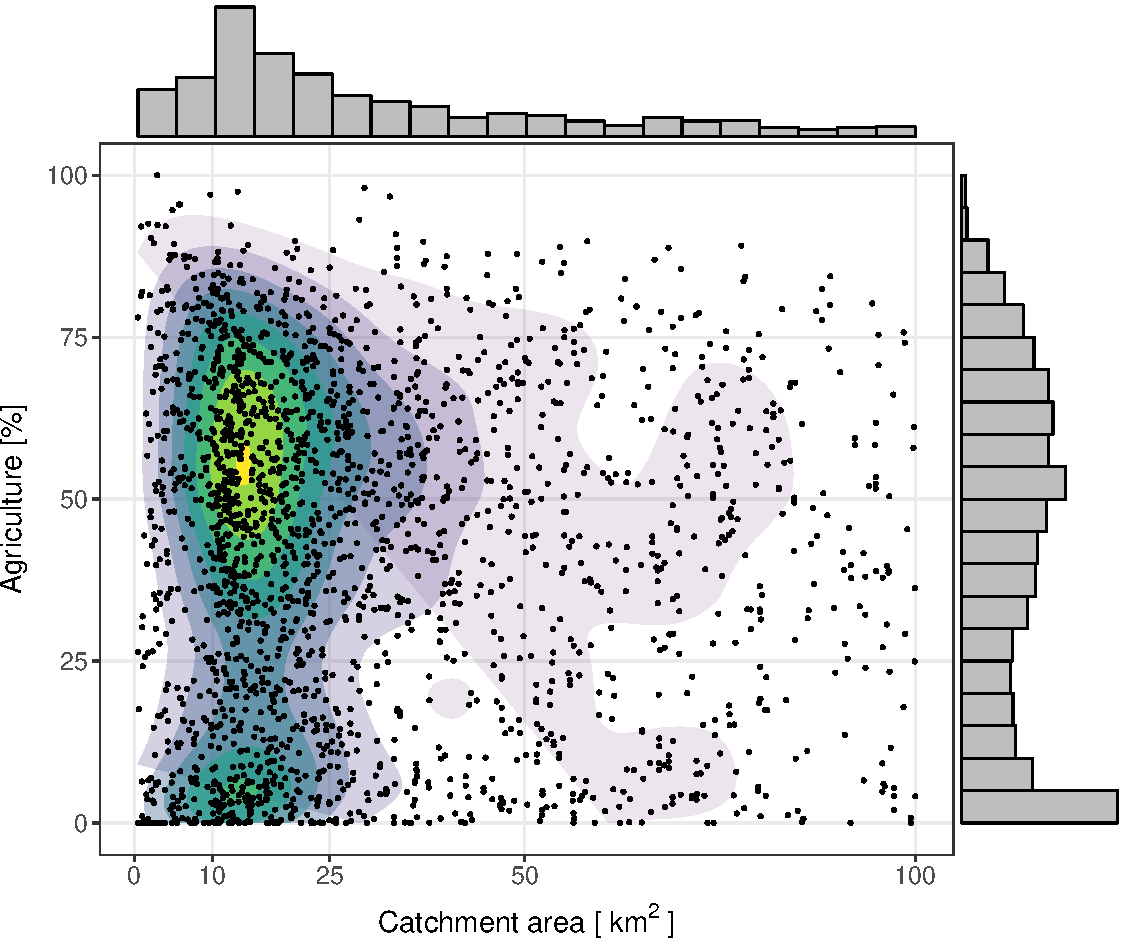
\includegraphics[width=\textwidth]{chapters/smallstreams/figure3.pdf}
  \caption[Distribution of catchment area and agriculture within the catchment area across the sampling sites.]{Distribution of catchment area and agriculture within the catchment area across the sampling sites.
  Colour codes the 2-dimensional density of points.}
  \label{fig:ss:fig3}
\end{figure}


\subsection{Influence of agricultural land use and catchment size}
The number of RAC exceedances increased strongly and statistically significant up to 28\% agriculture within the catchment.
The mean number of RAC exceedances per site increased 3.7-fold from 0.10 (no agriculture) to 0.39 (28\% agriculture within the catchment). 
Above this threshold the exceedances levelled.
Above 75\% agriculture within the catchment the number of exceedances further increased, but the increase was not statistically significant (Figure~\ref{fig:ss:fig4}, left). 
Catchment size had no statistically significant effect on the number of RAC exceedances (Figure~\ref{fig:ss:fig4}, right).
We also could not detect a statistically significant interaction between catchment size and agriculture. 

\begin{figure}[ht]
  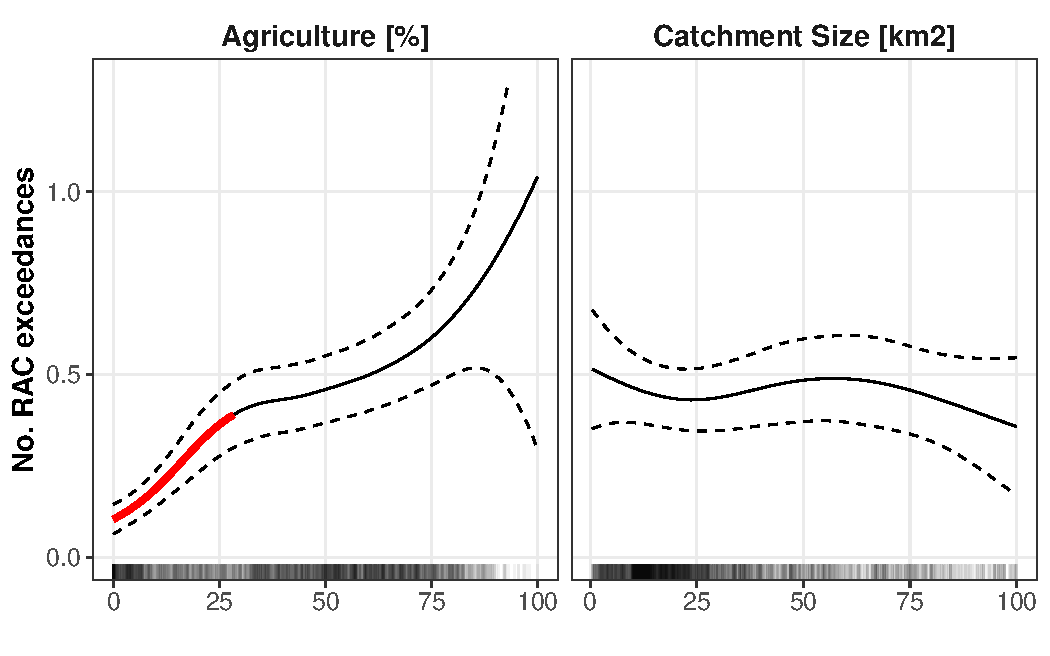
\includegraphics[width=\textwidth]{chapters/smallstreams/figure4.pdf}
  \caption[Effect of percent agriculture within the catchment and catchment size on the number of RAC exceedances.]{Effect of percent agriculture within the catchment (left) and catchment size (right) on the number of RAC exceedances. Red line marks statistically significant changes. Dashed lines denote 95\% point-wise Confidence Intervals.
  }
  \label{fig:ss:fig4}
\end{figure}


\subsection{Effect of precipitation on pesticide risk}
The spatio-temporal intersection revealed that most samples were taken during periods of low precipitation.
For example, only 5\% of the samples were taken at or after days with rainfall events greater than 10mm / day that may lead to run-off (Supplemental Figure~S6). 

$prec_{0}$ and $prec_{-1}$ increased the probability of exceeding LOQ and RQ.
In $Q2$ an increase from 0.1~mm to 10~mm of precipitation before sampling ($prec_{-1}$) lead on average to a 36\% higher mean RQ of 0.05.
The probability to exceed LOQ increases 1.6-fold from 8.7\% to 13.5\% (Figure~\ref{fig:ss:fig5}, top). % do_precip.R
Effects differed between individual compounds and are provided in the Supplemental Table~S4. 
Precipitation before sampling ($prec_{-1}$) had a stronger effect than precipitation during sampling ($prec_{0}$) on the probability of exceeding LOQ. 
This difference was less pronounced for the mean value of RQ (Figure~\ref{fig:ss:fig5}, top). 

The first quarter showed the lowest RQ and probability of exceeding LOQ.
Both increased during summer months and decreased towards the end of the year.
There was a 2.5-fold higher probability of exceeding LOQ in $Q2$ (10.6\%) than in $Q1$ (4.6\%).
The differences were less pronounced for the mean value of RQ and with less precision (Figure~\ref{fig:ss:fig5}, bottom). 
Individual compounds showed different temporal patterns (see Supplemental Table~S4). 


\begin{figure}[ht]
  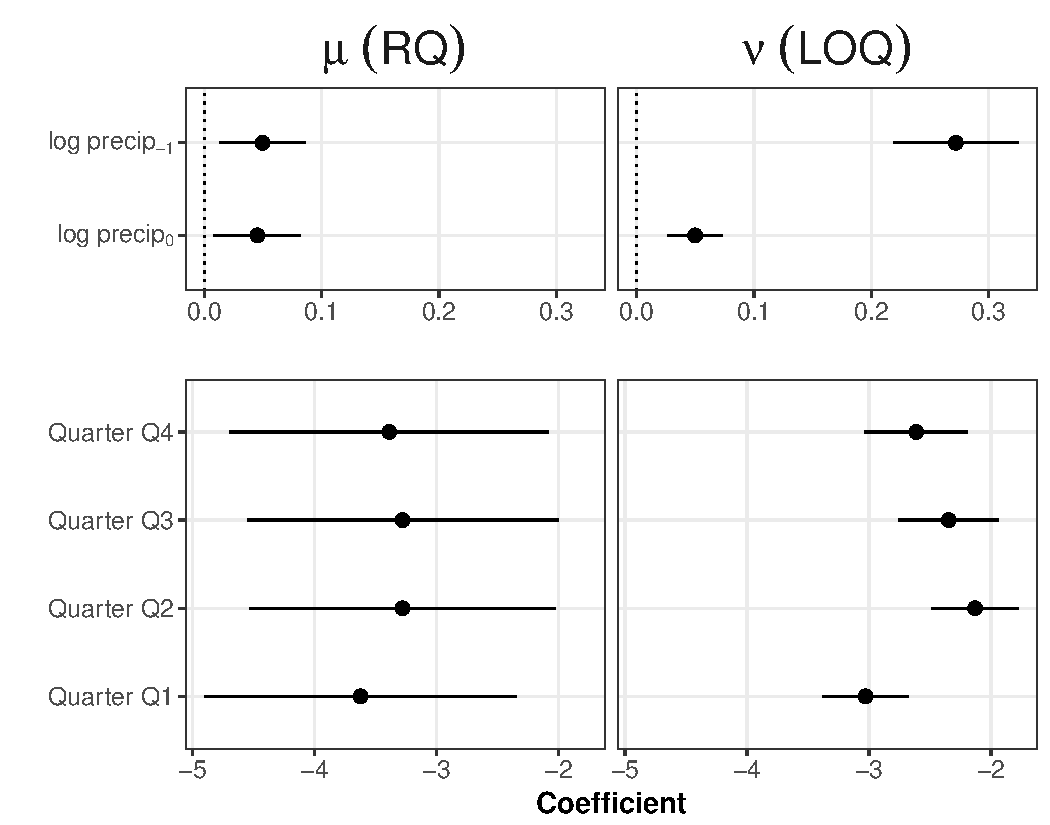
\includegraphics[width=\textwidth]{chapters/smallstreams/figure5.pdf}
  \caption[Summarised coefficients (and their 95\% CI) for precipitation (top row) and quarter (bottom row) from a meta-analysis of the 22 modelled compounds.]{Summarised coefficients (and their 95\% CI) for precipitation (top row) and quarter (bottom row) from a meta-analysis of the 22 modelled compounds. Left: coefficients for mean RQ ($\mu$), right: coefficients for probability of exceeding LOQ ($\nu$). 
  Coefficients are shown on the link scale (see Eq.~\ref{eqn:eqn4}).
  Single compound coefficients are provided in Supplemental Table~S4 and Figure~S7).
  }
  \label{fig:ss:fig5}
\end{figure}



\subsection{Pesticide risk in small streams}
We found RAC exceedances in 25.5\% of sampling sites and RQ > 0.1 in 54\% of sites. 
In 23\% of sites none of the chemicals, for which RACs were available, were detected (see also Supplemental Figure~S8).
Neonicotinoid insecticides and Chlorpyrifos showed the highest RQ (Figure~\ref{fig:ss:fig6}). %do_pollution.R
For Thiacloprid and Chlorpyrifos the RAC was equal or less than LOQ, therefore, all detections have a $RQ \ge 1$. 
The herbicides Nicosulfuron and Diflufenican, as well as the fungicide Dimoxystrobin also showed high exceedances of RQ (26.7, 14.1 and 21.1 \% of measurements~\textgreater~LOQ), see also Supplemental Table~S5).
RAC exceedances were found in 14\% of samples with concentrations \textgreater LOQ (and 7.3\% of all samples).

The highest RQs were observed for Chlorpyrifos (max(RQ) = 220), Clothianidin (max(RQ) = 157), Dimoxystrobin(max(RQ) = 117) and Isoproturon (max(RQ) = 80). 
Where analysed, metabolites exhibited the highest detection rates (for example, Metazachlor sulfonic acid was detected in 84\% of all samples where it was analysed (n = 3038, see also Supplemental Figure~S9).
Glyphosate was the compound with the highest detection rates (41\%, n = 3557 samples), followed by Boscalid (23\%, n = 9886) and Isoproturon (22\%, n = 19112). 
However, only the latter showed RAC exceedances (Figure~\ref{fig:ss:fig6}).
In 45.9\% of samples more than one compound was quantified, with a maximum of 54 different compounds in one sample (Supplemental Figure~S10). 

\begin{figure}[H]
  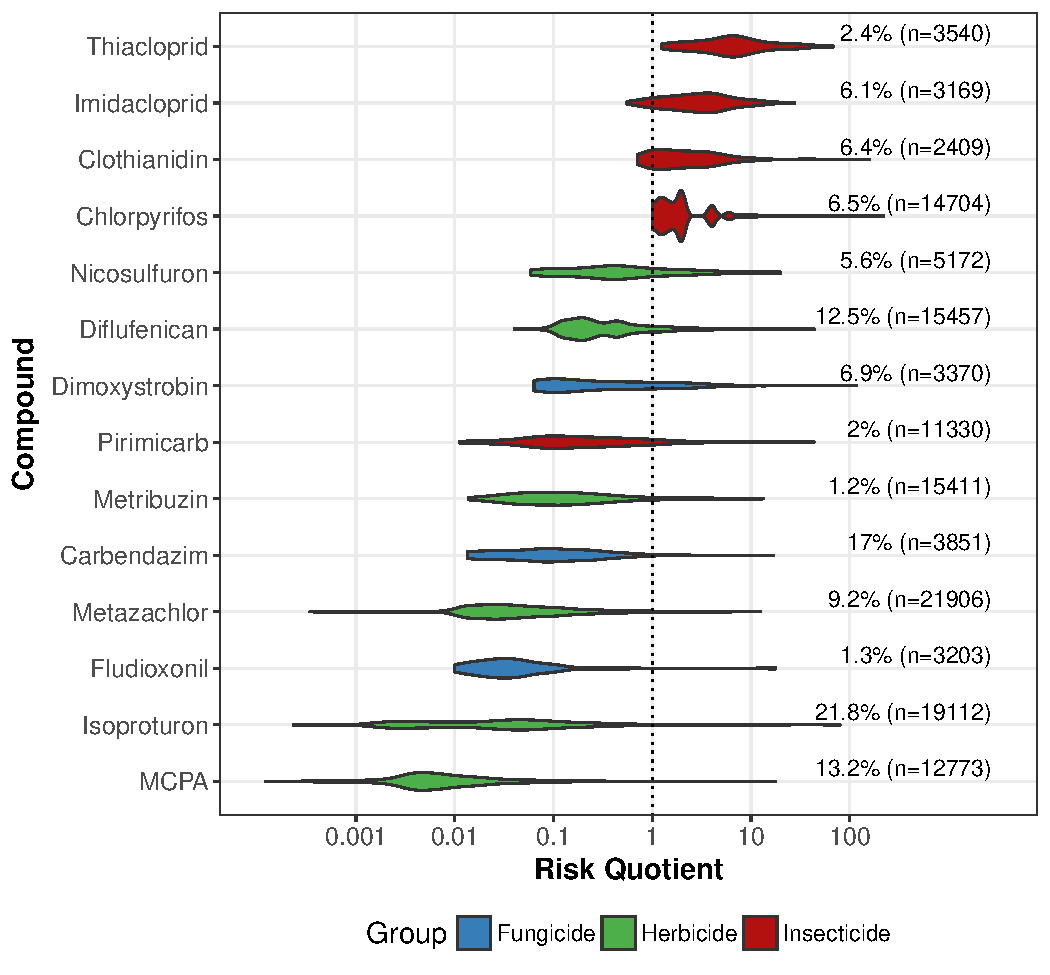
\includegraphics[width=0.9\textwidth]{chapters/smallstreams/figure6.pdf}
  \caption[15 compounds with the highest risk quotients in small streams.]{15 compounds with the highest risk quotients in small streams. Non-detects are not shown due to the logarithmic axis. Numbers on the right give the percentage of values \textgreater LOQ and the total number of samples were the compound was analysed.
  }
  \label{fig:ss:fig6}
\end{figure}




%% -------------------------------------------------------------------------
\section{Discussion}
\subsection{Overview on the compiled dataset}
The compiled dataset of governmental monitoring data, with a particular focus on small streams, represents currently the most comprehensive available for Germany.
Similar nationwide datasets have been compiled for the Netherlands \citep{vijver_spatial_2008}, Switzerland \citep{munz_pestizidmessungen_2011} and the United States \citep{stone2014pesticides}.
While the compilations from Europe are of similar quantity and quality to the  data compiled and analysed here, the compilation used in \citet{stone2014pesticides} is much smaller, though these data may be complemented by more data in future analyses. 

% current problems in monitoring and possible solutions
A nationwide assessment of pesticide pollution is hampered by inhomogeneous data across federal states:
Beside large differences in the spatial distribution and quantity of sampling sites (Figure~\ref{fig:ss:fig1}), the spectrum of analysed compounds (Figure~\ref{fig:ss:fig2}) and the quality of chemical analyses differed between states. 
Despite the outlined differences between states, all ecoregions occurring in Germany \citep{illies1978limnofauna,abell2008freshwater} were covered by the presented dataset and thus it might nonetheless represent a sample covering all types of small streams in Germany. 
For Thiacloprid and Chlorpyrifos the LOQs were above the RAC, which means that exceedances are likely underestimated.
For these compounds a lowering of LOQ through an improvement of chemical analysis is essential for reliable assessment.
Moreover, a nationwide assessment would benefit from a harmonised spectrum of analysed compounds between federal states. 

Given their high abundance in the landscape \citep{nadeau_hydrological_2007} small streams below 10~km\textsuperscript{2} are disproportionally less sampled in current monitoring (Figure~\ref{fig:ss:fig3}), which may be attributed to the missing categorisation in the WFD. 
Clearly, there is currently a lack of knowledge on stressor effects on small streams.
We analysed only data from small streams, however, for lentic small water bodies this lack might be even greater \citep{lorenz_specifics_2016}. 



\subsection{Influence of agricultural land use and catchment size}
% agriculture
We found a strong influence of agriculture on the pollution of streams.
Above 25\% agriculture within a catchment, it is likely that a RAC will be exceeded, with a further increase in entirely agricultural catchments (above 75 \% agriculture).
To our knowledge, this is the first study investigating such thresholds of pesticide risk.
Previous studies examined thresholds for the percentage of agricultural land use with respect to the response of biological communities, integrating different agricultural stressors.
\citet{feld_response_2013} found change points of biological community metrics at 40\% agricultural land use in lowland streams in Europe.
Similarly, \citet{waite_agricultural_2014} found a threshold for aquatic diatoms at 40\% agricultural land use in wadeable streams in the United States.
Our results coincide with these thresholds and suggest that pesticides might contribute to the observed biological changes. 

% size
We did not find a statistically significant relationship between pesticide pollution and catchment size.
However, previous studies showed that small streams are more polluted than bigger streams \citep{schulz_field_2004,stehle_pesticide_2015,knauer_pesticides_2016}.
This can be explained by the relatively short gradient of catchment sizes in our dataset, with most of the streams with catchments above $10~km^2$ and below $100~km^2$ (Figure~\ref{fig:ss:fig3}, top).
For example, the gradient of \citet{schulz_field_2004} covered 6 orders of magnitude.


\subsection{Effect of precipitation on pesticide risk}
Our results revealed that pesticide sampling for chemical monitoring in Germany is mainly performed when no precipitation occurs. 
Nevertheless, we found a 36\% higher RQ if samples were taken after rainfall events. 
Samples taken on the day of a rainfall event showed less risk than samples taken one day after a rainfall event.
This could be explained by the sampling preceding the rainfall event and the delay between the start of a rain event and the peak in discharge or runoff. 
The effects of precipitation were more pronounced for the probability to exceed LOQ, with smaller effect sizes for the absolute value of RQ. 
This may be explained by a higher variability of absolute concentrations.
Overall, our results indicate that current pesticide monitoring relying on grab sampling, largely disconnected from precipitation events, underestimates pesticide risks.
Automatic event-driven samplers \citep{stehle_probabilistic_2013} and passive samplers \citep{fernandez_calibration_2014,moschet_evaluation_2015} may help overcome these shortcomings and provide a better representation of risks, especially for small water bodies \citep{lorenz_specifics_2016}. 

We found the highest the probability of exceeding LOQ during summer (10\% for Q2) and lowest in the first quarter of the year (4\%, Figure~\ref{fig:ss:fig5}, bottom right).
This annual pattern coincides with the main application season for pesticides in Central Europe.
Nevertheless, there are compound-specific differences in the annual pattern, which explains the wide CI for the absolute RQ (Figure~\ref{fig:ss:fig5}, bottom left). 
For example, the herbicide Diflufenican showed the highest RQ and the highest probability of exceeding LOQ during the winter quarters Q1 and Q4 (Supplemental Table~S4), which coincides with the application period it is registered for in Germany \citep{bvl_online_2016}.
Our study suggests that pesticide risks display compound specific spatio-temporal dynamics.
Currently, little is known about these and further research on those might provide useful information for future ecological risk assessment. 
For example, the sensitivity of organisms is often life stage dependent \citep{hutchinson1998analysis} and knowledge on temporal dynamics could inform on concurrent exposure to multiple pesticides, as well as assist to parameterise toxicokinetic and toxicodynamic models \citep{ashauer2016modelling}. 
Moreover, our results show that analysing absolute concentrations and probabilities of LOQ together might deliver valuable insights into risk dynamics.


\subsection{Pesticides in small streams}
Our results suggest that small streams are frequently exposed to ecologically relevant pesticide concentrations.
In one-quarter of small streams RACs were exceeded at least once.
\citet{stehle_pesticide_2015} found the highest percentage of RAC exceedances for organophosphate insecticides. 
By contrast, we found that neonicotinoid insecticides have highest exceedances of RACs, followed by the organophosphate chlorpyrifos. 
This difference can be attributed to the low sample size for neonicotinoid insecticides in their study (n = 33) compared to the dataset presented here (for example 3,540 samples of Thiacloprid, Figure~\ref{fig:ss:fig6}). 
Overall, our results suggest that neonicotinoids may currently pose a high risk to freshwater ecosystems. 
Moreover, our results add further evidence to the growing literature on the risks arising from neonicotinoids for aquatic \citep{morrissey2015neonicotinoid} and terrestrial \citep{pisa2015effects} ecosystems. 

Compared to \citet{stehle_pesticide_2015} we found higher rates of RAC exceedances for insecticides.
They found exceedances in 37.1\% of insecticide measurements \textgreater LOQ (n = 1352, 23 insecticides), whereas, we found exceedances in 67\% of insecticide measurements with RACs \textgreater LOQ (n = 1855, 22 insecticides). 
This could be attributed to different insecticides considered and different underlying RACs.
Our study has only 7 insecticides with RACs in common with the insecticides investigated by \citet{stehle_pesticide_2015}.
Moreover, all RACs were lower in our study (average difference = -0.71 $\mu g/L$, range = [-2.757; -0.005]). 
Nevertheless, it must be noted that the dataset compiled here comprised only samples from grab sampling, which may considerably underestimate pesticide exposure \citep{stehle_probabilistic_2013, Xing_Chow_Rees_Meng_Li_Ernst_Benoy_Zha_Hewitt_2013}. 


By contrast, \citet{knauer_pesticides_2016} found exceedances from monitoring data mainly for herbicides and fungicides and only one insecticide Chlorpyrifos\--methyl. \\
More\-over, RAC exceedances in Switzerland were generally lower and less abundant (for example 6 exceedances (=0.2\%) for Isoproturon with a maximum RQ of 2) compared to our results for Germany. 
This might reflect differences in pesticide use between countries, ecoregions and RACs used. 
From the definition of RAC it follows that if the concentration of a compound exceeds its RAC ecological effects are expected.
Indeed, \citet{stehle_agricultural_2015} found that the biological diversity of stream invertebrates was significantly reduced by 30\% at RQ = 1.12 and by 10\% at 1/10 of RAC.
We found RQ values greater than 1.12 in 25\% of small streams and RQ at 1/10 of RAC in 54\% of small streams. 
Consequently, we conclude that agricultural pesticides are on a large scale a major threat to small streams, the biodiversity they host and the services they provide. 
This threat may exacerbate because pesticides often occur in mixtures \citep{schreiner_pesticide_2016} and may co-occur with other stressors \citep{schafer_contribution_2016}. 

% Approval / Risk Assessment
Monitoring data, despite the outlined limitations, provides an opportunity to study large-scale environmental occurrence patterns of pesticides.
Furthermore, such nationwide compilations, may not only be used for governmental surveillance, but also to answer other questions, like validation of exposure modelling \citep{knabel_fungicide_2014}, retrospective evaluation of regulatory risk assessment \citep{knauer_pesticides_2016,stehle_pesticide_2015}or occurrences of pesticide mixtures \citep{schreiner_pesticide_2016}.
However, the sampling design needs to account for precipitation events to provide robust data. 
Our results suggest that exceedances of RACs are landscape dependent % = Zusammenhang RAC<->Agriculture
and therefore, pesticide regulation should account for landscape features. 
Moreover, the high exceedances of RACs indicate that greater efforts are needed to describe causal links, which may lead to further developments of the current authorisation procedure.

%% ----------------------------------------------------------------------------
\section{References}
\printbibliography[heading=none]


% ---------------------------------------------------------------------------
% webchem: An R Package to Retrieve Chemical Information from the Web
\def\dir{chapters/webchem}
% -*- root: ../../thesis.tex -*-





\chapter[webchem: An R Package to Retrieve Chemical Information]{webchem: An R Package to Retrieve Chemical Information from the Web}
\label{sec:webchem}  

\begin{sloppypar}
\bigskip
\underline{Eduard Szöcs\textsuperscript{a}} \& Ralf B. Schäfer\textsuperscript{a}

\bigskip
\small
\noindent 
\textsuperscript{a}Institute for Environmental Sciences, University Koblenz-Landau, Landau, Germany 

\bigskip 
\normalsize
\noindent
Accepted in \emph{Journal of Statistical Software}, 2016.

\end{sloppypar}
\newpage


%% ----------------------------------------------------------------------------
\section{Abstract}
A wide range of chemical information is freely available online, including identifiers, experimental and predicted chemical properties.
However, these data are scattered over various data sources and not easily accessible to researchers.
Manual searching and downloading of such data is time-consuming and error-prone.  
We developed the open-source R package webchem that allows users to automatically query chemical data from currently 11 web sources. 
These cover a broad spectrum of information.
The data are automatically imported into an R object and can directly be used in subsequent analyses.
webchem enables easy, structured and reproducible data retrieval and usage from publicly available web sources.
In addition, it facilitates data cleaning, identification and reporting of substances.
Consequently, it reduces the time researchers need to spend on chemical data compilation.

\section[Introduction]{Introduction}
Before each statistical analysis, data cleaning is often required to ensure good data quality.
Data cleaning is the process of detecting errors and inconsistencies in data sets \citep{Chapman_2005}.
In practice, the data cleaning step is often more time consuming than the subsequent statistical analysis, particularly, when the analysis relies on the joining of multiple data sources.

When dealing with chemical data sets (e.g.\ environmental monitoring data, toxicological data), a first step is often to validate the names of chemicals or to link them to unique codes that simplify subsequent querying and appending of compound-related physico-chemical or toxicological information.
Several web sources provide chemical names or link them to unique codes (see also section \emph{Data sources} below).
However, manual searching for each compound, often through a graphical web interface, is tedious, error-prone and not reproducible \citep{Peng_2009}.

To simplify, robustify and automate this task, i.e.\ to search and retrieve chemical information from the web, we created the webchem package for the free and open source R language \citep{r_2015, Wehrens_2011}.
R is one of the most widely used software environments for data cleaning, analysing and visualising data, and supports full reproducibility of each step \citep{Marwick_2016}.

In the following, we describe the basic functionality of the package and demonstrate with a few use cases how to clean and retrieve new data with webchem.


\section[Implementation and design details]{Implementation and design details}
The webchem package is written entirely in R and available under a MIT license.
The development repository is hosted on \citet{github} and a stable version is released on the official R repository \citep{cran}.
webchem is part of the rOpenSci project \citep{boettiger2015building}, which aims at fully reproducible data analysis.

webchem follows best practices for scientific software \citep{wilson_best_2014, poisot_best_2015}, namely: (i) a public available repository with easy collaboration and an issue tracker (via GitHub), (ii) a non-restrictive license, version control (git), (iii) an elaborate test-suite covering more than 90\% of the relevant lines of code (currently approximately 1500 lines, using testthat \citep{wickham_testthat:_2011}), (iv) continuous integration (via \citet{travis-ci} and \citet{appveyor}; testing on Linux \& Windows with current and development R versions), (v) in-source documentation (using roxygen2 \citep{wickham_roxygen2:_2015}) and (vi) compliance with a style guide \citep{wickham_advanced_2015}.

webchem builds on top of the following R packages:
RCurl \citep{lang_rcurl:_2015} and httr \citep{wickham_httr} for data transfer,
stringr \citep{wickham_stringr:_2015} for string handling,
xml2 \citep{wickham_xml2} and rvest \citep{wickham_rvest} for parsing HTML and XML,
jsonlite \citep{ooms_jsonlite_2014} for parsing JSON,
rcdk \citep{guha_rcdk} for parsing SMILES.
For parsing molfiles we use a lightweight implementation of \citep{Grabner_Varmuza_Dehmer_2012}.

Some data sources provide application programming interfaces (API).
Web APIs define functions that allow accessing services and data via http and return data in a specific way.
webchem uses the API of a data source provider, where available.
For sources where an API is lacking, data is directly searched and extracted from the web pages, analogous to manual interaction with a website.

Only few design decisions have been made:
Each function name has a prefix and suffix separated by an underscore \citep{Chamberlain_Szocs_2013}.
They follow the format of source\_function, e.g.\ cs\_compinfo uses ChemSpider as source (see next section) to retrieve compound information.
Some functions require querying first a unique identifier from the data source and then use this identifier to query further information.
The prefix get is used to denote these functions, e.g.\ get\_csid to retrieve the identifier used in ChemSpider.

webchem is friendly to the resources of data providers. 
Between each request there is a time-out of 0.3 to 2 seconds depending on the data source. 
Therefore, processing of larger data sets can take some time, but still represents a major improvement compared to manual lookup.
We provide a link to the \emph{Terms of Use} of data providers in the documentation of each function and we encourage the users to read these before using webchem.
Moreover, all functions return an URL of the source, which can be used for \mbox{(micro-)attribution}.


\section[Data sources]{Data sources}
The backbone of webchem are data sources providing their data and functionality to the public.
Currently, data can be retrieved from 11 sources.
These cover a broad spectrum of available data, like identifiers, experimental and predicted properties and regulatory information (Figure~\ref{fig:fig1}, a detailed overview of all sources is included as supplement):

\begin{description}
  \item[NIH Chemical Identifier Resolver (CIR)]{A web service that converts \\from and to various chemical identifiers \citep{cir}.}
  \item[Chemical Translation Service (CTS)]{A web service that converts from and to various chemical identifiers \citep{wohlgemuth_haldiya_willighagen_kind_fiehn_2010}.}
  \item[ETOX]{Information System Ecotoxicology and Environmental Quality Targets by the German Federal Environmental Agency. Provides basic identifiers, synonyms, ecotoxicological data and quality targets for different countries \citep{etox}.}
  \item[PAN Pesticide Database]{Information on pesticides - provides basic identifiers, ecotoxicological data and chemical properties \citep{pan}.}
  \item[SRC Physprop]{Contains physical properties for over 41,000 chemicals.
  Physical properties collected from a wide variety of sources including experimental and modeled values\citep{physprop}.}
  \item[PubChem]{PubChem is a public repository for information on chemical substances, providing identifiers, properties and synonyms \citep{kim2016}.
  We use an interface to the PUG-REST web service \citep{Kim_Thiessen_Bolton_Bryant_2015}.}
  \item[Wikidata]{Wikipedia contains information for over 15,000 chemicals \citep{Ertl_Patiny_Sander_Rufener_Zasso_2015, wiki}. Currently webchem can only query chemical identifiers.}
  \item[Compendium of Pesticide Common Names]{The compendium provides information on pesticide common names, identifiers and classification \citep{wood}.}
  \item[ChemID\emph{plus}] {is a large web-based database provided by the National Library of Medicine (NLM). It provides identifiers, synonyms, toxicological data and chemical properties \citep{tomasulo2002}.}
  \item[ChemSpider]{is a free chemical structure database providing access to over 40 million structures. It provides identifiers, properties and can also be used to convert identifiers \citep{pence_chemspider:_2010}.}
  \item[OPSIN]{The Open Parser for Systematic IUPAC nomenclature is a chemical name interpreter and provides InChI and SMILES identifiers \citep{lowe_corbett_murray-rust_glen_2011}.}
\end{description}

Though the data sources exhibit some overlap in the provided information, each has been selected because it also provides unique information and we encourage the interested reader to consult the related source for details. 
However, we provide a brief overview in the Supporting Information.

\begin{figure}[H]
  \centering
  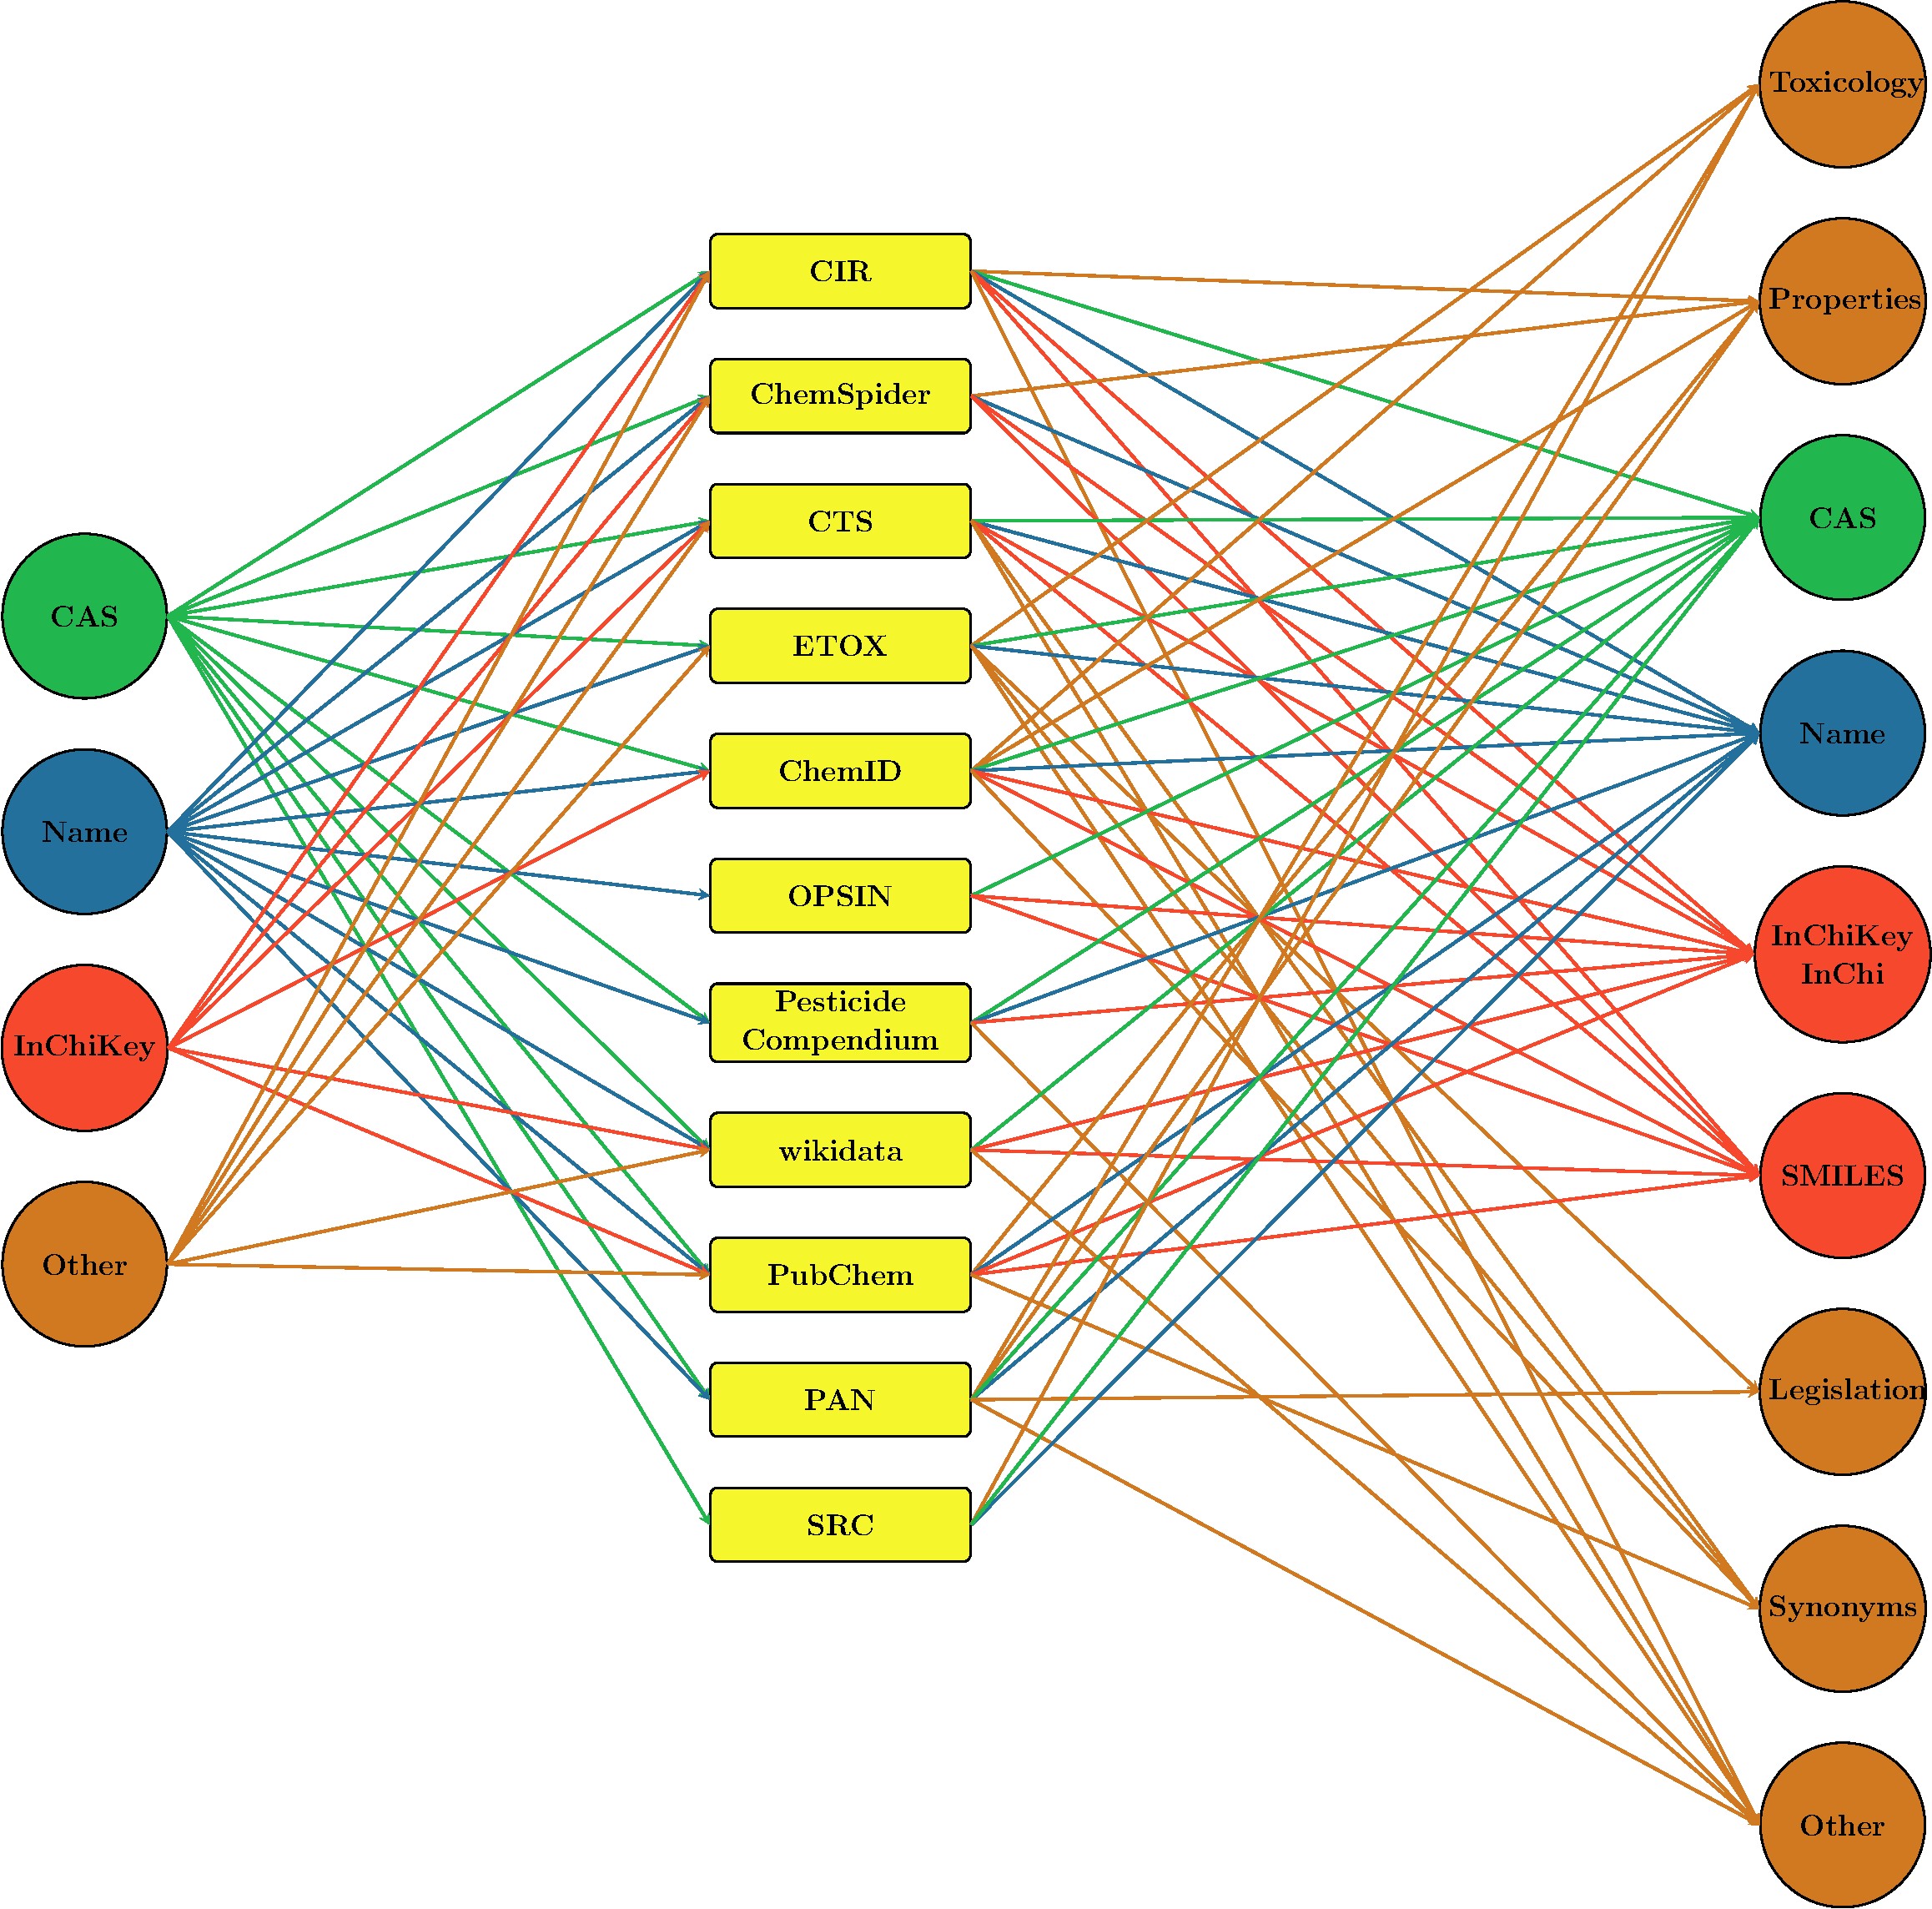
\includegraphics[width=\textwidth]{chapters/webchem/fig1.pdf}
  \caption[Overview of current data sources.]{Overview of current data sources. Input and output possibilities currently implemented in the package.}
  \label{fig:fig1}
\end{figure}

\newpage
\section[Use cases]{Use cases}
\subsection[Install webchem]{Installation}
webchem can be easily installed and loaded from CRAN:

\begin{knitrout}
\color{fgcolor}\begin{kframe}
\begin{alltt}
\hlstd{R> }\hlkwd{install.packages}\hlstd{(}\hlstr{"webchem"}\hlstd{)}
\hlstd{R> }\hlkwd{library}\hlstd{(}\hlstr{"webchem"}\hlstd{)}
\end{alltt}
\end{kframe}
\end{knitrout}




The package is under active development. The latest development version is available from GitHub and also permanently available at \citet{zenodo}.
This document has been created using webchem version 0.1.


\subsection[Sample data sets]{Sample data sets}
To demonstrate the capabilities of  webchem we use two small publicly available real world data sets.
The data sets are only used for purpose of demonstration, have been slightly preprocessed (not shown) and are available through the package.

(i) jagst: This data set comprises environmental monitoring data of organic substances in the river Jagst, Germany, sampled in 2013.
The data is publicly available and can be retrieved from \citet{lubw_2016}.
It comprises concentrations  (in $\mu g~/~L$) of  34 substances  on 13 sampling occasions.
First we load the data set and inspect the first six rows:

\begin{knitrout}
\color{fgcolor}\begin{kframe}
\begin{alltt}
\hlstd{R> }\hlkwd{data}\hlstd{(}\hlstr{"jagst"}\hlstd{)}
\hlstd{R> }\hlkwd{head}\hlstd{(jagst)}
\end{alltt}
\begin{verbatim}
##         date          substance value qual
## 1 2013-01-04 2,4-Dimethylphenol 0.006    <
## 2 2013-01-29 2,4-Dimethylphenol 0.006    <
## 3 2013-02-26 2,4-Dimethylphenol 0.006    <
## 4 2013-03-26 2,4-Dimethylphenol 0.006    <
## 5 2013-04-23 2,4-Dimethylphenol 0.006    <
## 6 2013-05-22 2,4-Dimethylphenol 0.006    <
\end{verbatim}
\end{kframe}
\end{knitrout}

This data set identifies substances only by substance names. Values below the limit of quantification (LOQ) are indicated by a qualifier column.

(ii) lc50: This data consists of median acute lethal concentration for the water flea \textit{Daphnia magna} in 48 h tests ($LC_{50, D.magna, 48h}$) of 124 insecticides.
The data has been retrieved from the EPA ECOTOX database \citep{epa_2016}.

\begin{knitrout}
\color{fgcolor}\begin{kframe}
\begin{alltt}
\hlstd{R> }\hlkwd{data}\hlstd{(}\hlstr{"lc50"}\hlstd{)}
\hlstd{R> }\hlkwd{head}\hlstd{(lc50)}
\end{alltt}
\begin{verbatim}
##        cas        value
## 4  50-29-3    12.415277
## 12 52-68-6     1.282980
## 15 55-38-9    12.168138
## 18 56-23-5 35000.000000
## 21 56-38-2     1.539119
## 36 57-74-9    98.400000
\end{verbatim}
\end{kframe}
\end{knitrout}

This data set identifies the substances only by CAS numbers.


\subsection[Query identifiers]{Query identifiers}
The jagst data set covers 34 substances that are identified by (German) names.
Merging and linking these to other tables is hampered by differences and ambiguity in compound names.

One possibility to resolve this, is to use different chemical identifiers allowing easy identification.
There are several identifiers available, e.g.  registry numbers like CAS or EC, database identifiers like PubChemCID \citep{kim2016} or ChemSpiderID \citep{pence_chemspider:_2010}, line notations like SMILES \citep{Weininger_1990}, InChI and InChiKey \citep{Heller_McNaught_Pletnev_Stein_Tchekhovskoi_2015}. 
In this first example we query several identifiers to create a table that can be used as (i) supplemental information to a research article or (ii) to facilitate subsequent matching with other data.

As we are are dealing with German substance names we start to query ETOX for CAS registry numbers.
A common work flow when dealing with web resources is to 1) query a unique identifier of the source, 2) use this identifier to retrieve additional information and 3) extract the parts that are needed from the R object \citep{Chamberlain_Szocs_2013}.

First we search for ETOX internal ID numbers using the substance names:

\begin{knitrout}
\small
\color{fgcolor}\begin{kframe}
\begin{alltt}
\hlstd{R> subs} \hlkwb{<-} \hlkwd{unique}\hlstd{(jagst}\hlopt{$}\hlstd{substance)}
\hlstd{R> ids} \hlkwb{<-} \hlkwd{get_etoxid}\hlstd{(subs,} \hlkwc{match} \hlstd{=} \hlstr{'best'}\hlstd{)}
\hlstd{R> }\hlkwd{head}\hlstd{(ids)}
\end{alltt}
\begin{verbatim}
##   etoxid                           match distance                  query
## 1   8668     2,4-Dimethylphenol ( 8668 )        0     2,4-Dimethylphenol
## 2   8494 4-Chlor-2-methylphenol ( 8494 )        0 4-Chlor-2-methylphenol
## 3   <NA>                            <NA>     <NA>     4-para-nonylphenol
## 4   8397                Atrazin ( 8397 )        0                Atrazin
## 5   7240                 Benzol ( 7240 )        0                 Benzol
## 6   7331        Desethylatrazin ( 7331 )        0        Desethylatrazin
\end{verbatim}
\end{kframe}
\end{knitrout}

Only three substances could not be found in ETOX. 
Here we specify that only the \emph{`best'} match (in terms of the Levenshtein distance between query and results) is returned. 
A manual check confirms appropriate matches. 
Other options include: \emph{`all'} - returns all matches; \emph{`first'} - returns only the first match (not necessarily the best match); \emph{`ask'} - this enters an interactive mode, where the user is asked for a choice if multiple matches are found and \emph{`na'} which returns NA in case of multiple matches.

We use these data to retrieve basic information on the substances.

\begin{knitrout}
\color{fgcolor}\begin{kframe}
\begin{alltt}
\hlstd{R> etox_data} \hlkwb{<-} \hlkwd{etox_basic}\hlstd{(ids}\hlopt{$}\hlstd{etoxid)}
\end{alltt}
\end{kframe}
\end{knitrout}

webchem always returns a named list (one entry for each substance) and the available information content can be very voluminous.
Therefore, we provide extractor functions for the common identifiers: CAS, SMILES and InChIKeys.
\begin{knitrout}
\small
\color{fgcolor}\begin{kframe}
\begin{alltt}
\hlstd{R> etox_cas} \hlkwb{<-} \hlkwd{cas}\hlstd{(etox_data)}
\hlstd{R> }\hlkwd{head}\hlstd{(etox_cas)}
\end{alltt}
\begin{verbatim}
##        8668        8494        <NA>        8397        7240        7331 
##  "105-67-9" "1570-64-5"          NA "1912-24-9"   "71-43-2" "6190-65-4"
\end{verbatim}
\end{kframe}
\end{knitrout}

A variety of data are available and we cannot provide extractor functions for each of those.
Therefore, if users need to extract other data, they have to write simple extractor functions (see following examples).

In the same manner, we can now query other identifiers from another source using these CAS numbers (Figure~\ref{fig:fig1}), like PubChem


\begin{knitrout}
\color{fgcolor}\begin{kframe}
\begin{alltt}
\hlstd{R> cids} \hlkwb{<-} \hlkwd{get_cid}\hlstd{(etox_cas)}
\hlstd{R> pc_data} \hlkwb{<-} \hlkwd{pc_prop}\hlstd{(cids,} \hlkwc{properties} \hlstd{=} \hlkwd{c}\hlstd{(}\hlstr{'CanonicalSMILES'}\hlstd{))}
\hlstd{R> pc_smiles} \hlkwb{<-} \hlkwd{smiles}\hlstd{(pc_data)}
\end{alltt}
\end{kframe}
\end{knitrout}

or ChemSpider
\begin{knitrout}
\color{fgcolor}\begin{kframe}
\begin{alltt}
\hlstd{R> csids} \hlkwb{<-} \hlkwd{get_csid}\hlstd{(etox_cas,} \hlkwc{token} \hlstd{= token)}
\hlstd{R> cs_data} \hlkwb{<-} \hlkwd{cs_compinfo}\hlstd{(csids,} \hlkwc{token} \hlstd{= token)}
\hlstd{R> cs_inchikey} \hlkwb{<-} \hlkwd{inchikey}\hlstd{(cs_data)}
\end{alltt}
\end{kframe}
\end{knitrout}

Finally, we combine the queried data into one data.frame
\begin{knitrout}
\color{fgcolor}\begin{kframe}
\begin{alltt}
\hlstd{R> res} \hlkwb{<-} \hlkwd{data.frame}\hlstd{(}\hlkwc{name} \hlstd{= subs,} \hlkwc{cas} \hlstd{= etox_cas,} \hlkwc{smiles} \hlstd{= pc_smiles,}
  \hlkwc{cid} \hlstd{= pc_data}\hlopt{$}\hlstd{CID,} \hlkwc{inchikey} \hlstd{= cs_inchikey,} \hlkwc{csid} \hlstd{= cs_data}\hlopt{$}\hlstd{csid,}
  \hlkwc{stringsAsFactors} \hlstd{=} \hlnum{FALSE}\hlstd{)}
\end{alltt}
\end{kframe}
\end{knitrout}

Note that in order to use the ChemSpider functions, a personal authentication key (token) is needed, which can be retrieved from the ChemSpider web page. 
Finally, we obtain a compound table containing many different identifiers (Table~\ref{tab:comptable}), allowing easy identification and merging with other data sets, e.g.\ the lc50 data set based on CAS.

\begin{table}[ht]
\centering
\small
% latex table generated in R 3.3.1 by xtable 1.8-2 package
% Mon Oct 24 17:58:49 2016
\begin{tabular}{R{3.2cm}lllll}
  \toprule
Name & CAS & SMILES & CID & InChIKey & CSID \\ 
  \midrule
2,4-Dimethylphenol & 105-67-9 & CC1=CC(... & 7771 & KUFFULV... & 13839123 \\ 
  4-Chlor-2-methylphenol & 1570-64-5 & CC1=C(C... & 14855 & RHPUJHQ... & 14165 \\ 
  4-para-nonylphenol & - & - & - & - & - \\ 
  Atrazin & 1912-24-9 & CCNC1=N... & 2256 & MXWJVTO... & 2169 \\ 
  Benzol & 71-43-2 & C1=CC=C... & 241 & UHOVQNZ... & 236 \\ 
  Desethylatrazin & 6190-65-4 & CC(C)NC... & 22563 & DFWFIQK... & 21157 \\ 
   \bottomrule
\end{tabular}

\caption[Identifiers for the jagst data sets as queried with webchem.]{Identifiers for the jagst data sets as queried with webchem. Only the first 6 entries are shown. For SMILES and InChIKey only the first 7 characters are shown. - = not found.}
\label{tab:comptable}
\end{table}



\subsection[Toxicity of different pesticide groups]{Toxicity of different pesticide groups}
Another question we might ask is \emph{How does toxicity vary between insecticide groups?}
Answering this question would require tedious lookup of insecticide groups for each of the 124 CAS numbers in the lc50 data set.
The Compendium of Pesticide Common Names \citep{wood} contains such information and can be easily queried using CAS numbers with webchem: 

\begin{knitrout}
\color{fgcolor}\begin{kframe}
\begin{alltt}
\hlstd{R> aw_data} \hlkwb{<-} \hlkwd{aw_query}\hlstd{(lc50}\hlopt{$}\hlstd{cas,} \hlkwc{type} \hlstd{=} \hlstr{'cas'}\hlstd{)}
\end{alltt}
\end{kframe}
\end{knitrout}

To extract the chemical group from the retrieved data set, we write a simple extractor function and apply this to the retrieved data:

\begin{knitrout}
\color{fgcolor}\begin{kframe}
\begin{alltt}
\hlstd{R> igroup} \hlkwb{<-} \hlkwd{sapply}\hlstd{(aw_data,} \hlkwa{function}\hlstd{(}\hlkwc{y}\hlstd{) y}\hlopt{$}\hlstd{subactivity[}\hlnum{1}\hlstd{])}
\hlstd{R> igroup[}\hlnum{1}\hlopt{:}\hlnum{3}\hlstd{]}
\end{alltt}
\begin{verbatim}
##                                   50-29-3 
##             "organochlorine insecticides" 
##                                   52-68-6 
##                "phosphonate insecticides" 
##                                   55-38-9 
## "phenyl organothiophosphate insecticides"
\end{verbatim}
\end{kframe}
\end{knitrout}

Figure \ref{fig:fig2} displays the result after additional data cleaning (see supplement for full code).
Overall, it took only 5 R statements to retrieve, clean and plot the data using ggplot2 \citep{ggplot2}.

\begin{figure}[ht]
\begin{knitrout}
\color{fgcolor}

{\centering 
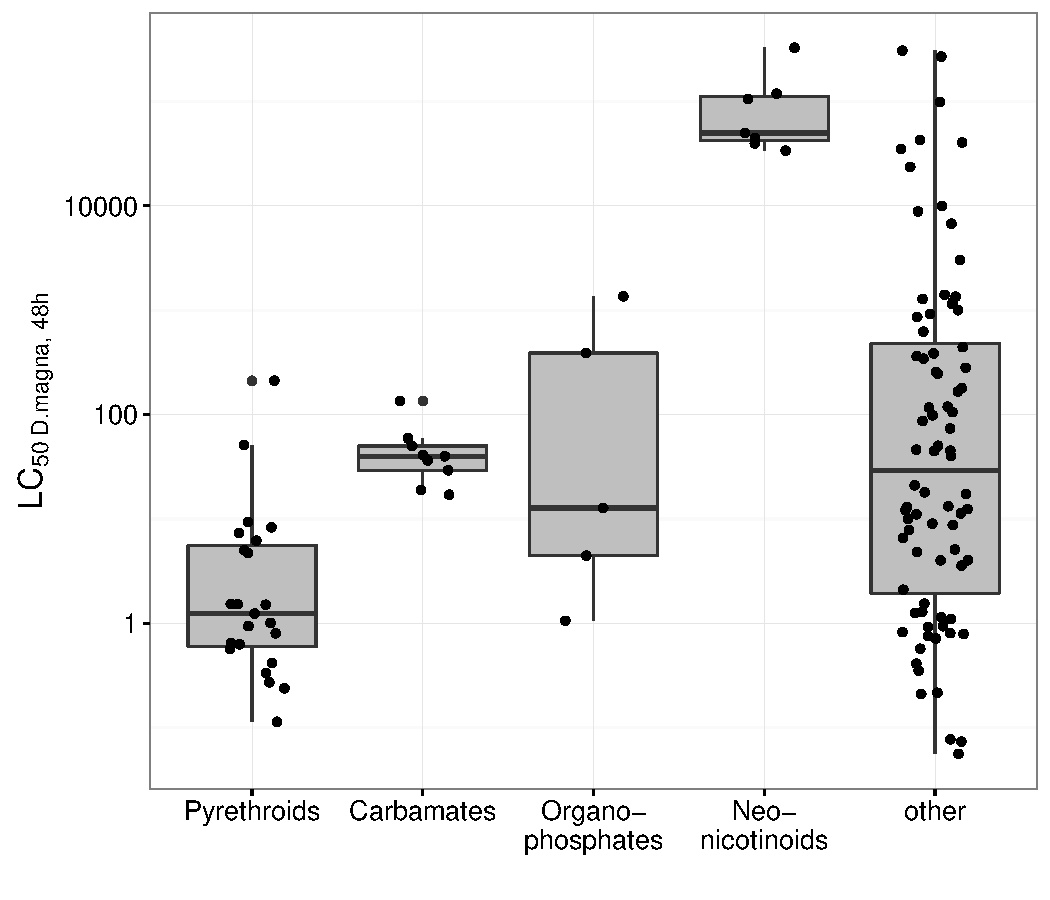
\includegraphics[width=0.7\textwidth]{chapters/webchem/plot_lc50-1.pdf}
}



\end{knitrout}
\caption[Toxicity of different pesticide groups.]{Toxicity of different pesticide groups. LC\textsubscript{50} values have been retrieved from EPA ECOTOX database, chemical groups from the Compendium of Pesticide Common Names.}
\label{fig:fig2}
\end{figure}


\subsection[Querying partitioning coefficients]{Querying partitioning coefficients}
Some data sources also provide data on chemical properties that can be queried.
Here we query for the lc50 data the $\mathrm{log}~P_{oct/wat}$ from the SRC PHYSPROP database to build a simple quantitative structure–activity relationship (QSAR) to predict toxicity.

\begin{knitrout}
\color{fgcolor}\begin{kframe}
\begin{alltt}
\hlstd{R> pp_data} \hlkwb{<-} \hlkwd{pp_query}\hlstd{(lc50}\hlopt{$}\hlstd{cas)}
\end{alltt}
\end{kframe}
\end{knitrout}

The database contains predicted and experimental values.
Extracting \\ $\mathrm{log}~P_{oct/wat}$ from the data object is slightly more complicated,  
because i) for some compounds no data could be found and ii) the data-object has a more complex structure (a data frame within a list).

\newpage
\begin{knitrout}
\color{fgcolor}\begin{kframe}
\begin{alltt}
\hlstd{R> lc50}\hlopt{$}\hlstd{logp} \hlkwb{<-} \hlkwd{sapply}\hlstd{(pp_data,} \hlkwa{function}\hlstd{(}\hlkwc{y}\hlstd{) \{}
  \hlkwa{if} \hlstd{(}\hlkwd{length}\hlstd{(y)} \hlopt{==} \hlnum{1} \hlopt{&&} \hlkwd{is.na}\hlstd{(y))}
    \hlkwd{return}\hlstd{(}\hlnum{NA}\hlstd{)}
  \hlstd{y}\hlopt{$}\hlstd{prop}\hlopt{$}\hlstd{value[y}\hlopt{$}\hlstd{prop}\hlopt{$}\hlstd{variable} \hlopt{==} \hlstr{'Log P (octanol-water)'}\hlstd{]}
\hlstd{\})}
\end{alltt}
\end{kframe}
\end{knitrout}

We opted for this more complex approach, because the information available is very diverse and we cannot provide an extractor function for each purpose.
Moreover, it provides users with high flexibility regarding organisation of their data. 
Nevertheless, in the documentation of each function we provide examples on how to extract more complicated parts of the data.
The resulting data and model is displayed in Figure~\ref{fig:fig3}.

\begin{figure}[ht]
\begin{knitrout}
\color{fgcolor}

{\centering 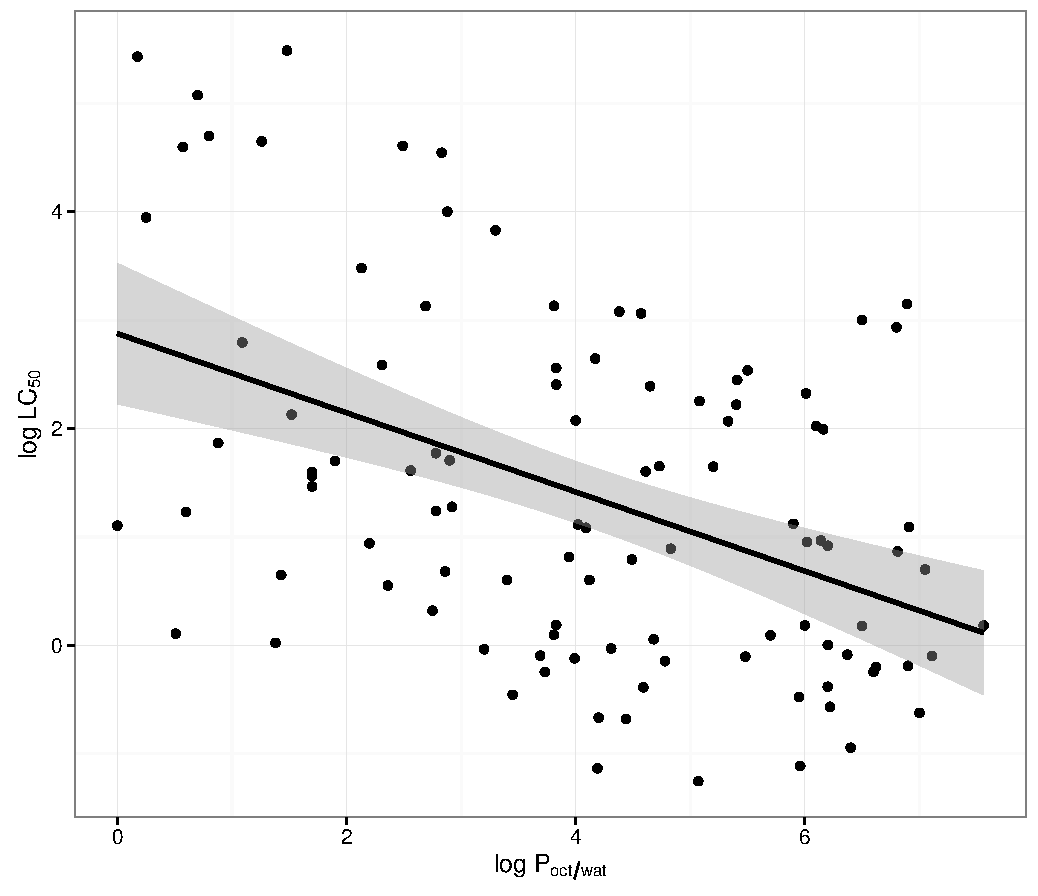
\includegraphics[width=0.7\textwidth]{chapters/webchem/plot_qsar-1.pdf} 

}



\end{knitrout}
\caption[Simple QSAR for predicting log LC\textsubscript{50} of pesticides by log P.]{Simple QSAR for predicting log LC\textsubscript{50} of pesticides by log P. 
Log P values have been retrieved from SRC Physprop database (97 experimental data, 9 estimated data and 18 substances without data). 
The line indicates the regression model ($\mathrm{log~LC}_{50} = 2.88\ensuremath{-0.37}~\mathrm{log} P$, RMSE = 1.45).}
\label{fig:fig3}
\end{figure}


\newpage
\subsection[Regulatory information]{Regulatory information}
Regulatory information is of particular interest if concentrations exceed national thresholds.
In the European Union (EU) the Water Framework Directive (WFD, \citet{wfd2000directive}) defines Environmental Quality Standards (EQS).
Similarly, the U.S. and Canadian EPA and the WHO define Quality Standards.
Information on these standards can be queried with webchem from the PAN Pesticide Database (using pan\_query()) and from ETOX (using etox\_targets()).

In this example we search for the minimum EQS for the EU for the compounds in the jagst data set, join these with measured concentrations and evaluate wether exceedances occurred..

We re-use the above queried ETOX-IDs to obtain further information from ETOX, namely the MAC-EQS:

\newpage
\begin{knitrout}
\color{fgcolor}\begin{kframe}
\begin{alltt}
\hlstd{R> eqs} \hlkwb{<-} \hlkwd{etox_targets}\hlstd{(ids}\hlopt{$}\hlstd{etoxid)}
\hlstd{R> ids}\hlopt{$}\hlstd{mac} \hlkwb{<-} \hlkwd{sapply}\hlstd{(eqs,} \hlkwa{function}\hlstd{(}\hlkwc{y}\hlstd{)\{}
  \hlkwa{if} \hlstd{(}\hlkwd{length}\hlstd{(y)} \hlopt{==} \hlnum{1} \hlopt{&&} \hlkwd{is.na}\hlstd{(y)) \{}
    \hlkwd{return}\hlstd{(}\hlnum{NA}\hlstd{)}
  \hlstd{\}} \hlkwa{else} \hlstd{\{}
    \hlstd{res} \hlkwb{<-} \hlstd{y}\hlopt{$}\hlstd{res}
    \hlkwd{min}\hlstd{(res[res}\hlopt{$}\hlstd{Country_or_Region} \hlopt{==} \hlstr{'EEC / EU'} \hlopt{&}
              \hlstd{res}\hlopt{$}\hlstd{Designation} \hlopt{==} \hlstr{'MAC-EQS'}\hlstd{,} \hlstr{'Value_Target_LR'}\hlstd{])}
  \hlstd{\}}
\hlstd{\})}
\end{alltt}
\end{kframe}
\end{knitrout}

Again, the returned information is humongous and we encourage users to study the returned objects and description of the data source.
Here, the column Designation defines the type of EQS and Value\_Target\_LR contains the value.
Unfortunately, we only found MAC-EQS values for 5 substances:

\begin{knitrout}
\color{fgcolor}\begin{kframe}
\begin{alltt}
\hlstd{R> (mac} \hlkwb{<-} \hlkwd{with}\hlstd{(ids, ids[}\hlopt{!}\hlkwd{is.na}\hlstd{(mac)} \hlopt{&} \hlkwd{is.finite}\hlstd{(mac),}
                      \hlkwd{c}\hlstd{(}\hlstr{'etoxid'}\hlstd{,} \hlstr{'query'}\hlstd{,} \hlstr{'mac'}\hlstd{)]))}
\end{alltt}
\begin{verbatim}
##    etoxid       query    mac
## 4    8397     Atrazin  2.000
## 5    7240      Benzol 50.000
## 11   8836     Irgarol  0.016
## 12   7442 Isoproturon  1.000
## 29   8756   Terbutryn  0.034
\end{verbatim}
\end{kframe}
\end{knitrout}

The get\_etoxid() function used to search ETOX-IDs returns also the original substance name (query),
so that we can easily join the table with MAC values with the measurements table :
\begin{knitrout}
\color{fgcolor}\begin{kframe}
\begin{alltt}
\hlstd{R> jagst_eqs} \hlkwb{<-} \hlkwd{merge}\hlstd{(jagst, mac,} \hlkwc{by.x} \hlstd{=} \hlstr{'substance'}\hlstd{,} \hlkwc{by.y} \hlstd{=} \hlstr{'query'}\hlstd{)}
\hlstd{R> }\hlkwd{head}\hlstd{(jagst_eqs)}
\end{alltt}
\begin{verbatim}
##   substance       date  value qual etoxid mac
## 1   Atrazin 2013-09-10 0.0068    =   8397   2
## 2   Atrazin 2013-10-08 0.0072    =   8397   2
## 3   Atrazin 2013-03-26 0.0040    =   8397   2
## 4   Atrazin 2013-04-23 0.0048    =   8397   2
## 5   Atrazin 2013-11-05 0.0036    =   8397   2
## 6   Atrazin 2013-07-16 0.0052    =   8397   2
\end{verbatim}
\end{kframe}
\end{knitrout}

Finally, we can compare the measured value to the MAC, which reveals that there have been no exceedances of these 5 compounds.




\subsection[Utility functions]{Utility functions}
Furthermore, webchem provides also basic functions to check identifiers that can be used for data quality assessment.
The functions either use simple formatting rules,

\begin{knitrout}
\color{fgcolor}\begin{kframe}
\begin{alltt}
\hlstd{R> }\hlkwd{is.inchikey}\hlstd{(}\hlstr{'BQJCRHHNABKAKU-KBQPJGBKS-AN'}\hlstd{)}
\end{alltt}


{\ttfamily\noindent\itshape\color{messagecolor}{\#\# Hyphens not at position 15 and 26.}}\begin{verbatim}
## [1] FALSE
\end{verbatim}
\begin{alltt}
\hlstd{R> }\hlkwd{is.cas}\hlstd{(}\hlstr{'64-17-6'}\hlstd{)}
\end{alltt}


{\ttfamily\noindent\itshape\color{messagecolor}{\#\# Checksum is not correct! 5 vs. 6}}\begin{verbatim}
## [1] FALSE
\end{verbatim}
\end{kframe}
\end{knitrout}

or web resources like ChemSpider
\begin{knitrout}
\color{fgcolor}\begin{kframe}
\begin{alltt}
\hlstd{R> }\hlkwd{is.inchikey}\hlstd{(}\hlstr{'BQJCRHHNABKAKU-KBQPJGBKSA-5'}\hlstd{,}
  \hlkwc{type} \hlstd{=} \hlstr{'chemspider'}\hlstd{)}
\end{alltt}
\begin{verbatim}
## [1] FALSE
\end{verbatim}
\end{kframe}
\end{knitrout}

\newpage
\section[Discussion]{Discussion}
\subsection[Related software]{Related software}
Within the R ecosystem, there are only a few similar projects:
rpubchem \citep{rpubchem_2014} provides an interface to PubChem.
Similarly, ChemmineR \citep{chemminer_2008}, a mature chemo-informatics package, provides an interface to Pubchem. 
webchem does not provide any chemo-informatic functionality, but integrates access to many data sources.
WikidataR \citep{wikidatar_2016} provides an interface to wikidata that could be used to retrieve chemical data from Wikipedia.
However, it does not provide predefined methods for chemical data like webchem.
Within the Python ecosystem the libraries PubChempy \citep{pubchempy}, ChemSpiPy \citep{chemspipy} and CIRpy \citep{cirpy} are available for similar tasks as those outlined here.
webchem is not specialized and tries to integrate many data sources and for some of these it provides a unique programmatic interface.
The Chemical Translation Service \citep{wohlgemuth_haldiya_willighagen_kind_fiehn_2010}, which is also one of the sources that can be queried, allows batch conversion of chemical identifiers.
However, it does not provide access to other data (experimental, modeled or regulatory data).


\subsection[Open Science]{Open Science}
An increasing number of scientific data is becoming publicly available \citep{Gewin_2016, Reichman_Jones_Schildhauer_2011,Boyle_Guha_2011}, either in public data repositories or as supplement to publications.
To be usable for other researchers chemical compounds should be properly identified, not only by chemical names but also with accompanying identifiers like InChIKey, SMILES and authority-assigned identifiers.
webchem provides an easy way to create such meta tables as shown in Table \ref{tab:comptable} and facilitates chemical data availability to researchers.
However, good quality of data is crucial for every analysis \citep{stieger2014} and additional effort and methods are needed to validate data quality.

\subsection[Further development]{Further development}
We have outlined only a few use cases that will likely be useful for many researchers.
Given the huge amount of publicly available information, many other possibilities can be envisioned.
webchem is currently under active development and several other data sources have not been implemented yet but may be in the future.
GitHub makes contributing easy and we strongly encourage contribution to the package.
Moreover, comments, feedback and feature requests are highly welcome.


\section[Conclusions]{Conclusions}
Researchers need to have easy access to global knowledge on chemicals.
webchem can save \emph{"hundreds of working hours"} gathering this knowledge \citep{munchalizia2016}, so that researchers can focus on other tasks.



%% ----------------------------------------------------------------------------
\newpage
\section{References}
\printbibliography[heading=none]


% ---------------------------------------------------------------------------
% taxize: taxonomic search and retrieval in R
\cleardoublepage
\def\dir{chapters/taxize}
% -*- root: ../../thesis.tex -*-

\chapter{taxize: taxonomic search and retrieval in R}
\label{sec:taxize} 
 
\begin{sloppypar}

\bigskip
Scott A. Chamberlain\textsuperscript{a} \& \underline{Eduard Szöcs\textsuperscript{b}}

\bigskip
\small
\noindent 
\textsuperscript{a}Biology Department, Simon Fraser University, Burnaby, BC, Canada,\\
\textsuperscript{b}Institute for Environmental Sciences, University Koblenz-Landau, Landau, Germany 

\bigskip 
\normalsize
\noindent 
Adapted from the article published in 2013 in \emph{F1000Research}, 2.191.

\bigskip
\noindent
This chapter reflects the software state in 2013.
In the meantime there have been many changes to taxize, so that not all parts presented here and thre respective supplementary materials work anymore. 
For a more recent description please visit the project homepage \url{https://github.com/ropensci/taxize}.

\end{sloppypar}

\newpage


%% ----------------------------------------------------------------------------
% be sloppy in this chapter
\begin{sloppypar}
\section{Abstract} 
\label{sec:taxize:abstract} 
All species are hierarchically related to one another, and we use taxonomic names to label the nodes in this hierarchy. 
Taxonomic data is becoming increasingly available on the web, but scientists need a way to access it in a programmatic fashion that's simple and reproducible. 
We have developed taxize, an open-source software package for the R language (freely available from \url{http://cran.r-project.org/web/packages/taxize}). 
taxize provides simple, programmatic access to taxonomic data for 13 data sources around the web. 
We discuss the need for a taxonomic toolbelt in R, and outline a suite of use cases for which taxize is ideally suited (including a full workflow as an appendix). 
The taxize package facilitates open and reproducible science by allowing taxonomic data collection to be done in the open-source R platform.

%% ----------------------------------------------------------------------------
\section{Introduction} 
\label{sec:taxize:introduction} 
Evolution by natural selection has led to a hierarchical relationship among all living organisms.  
Thus, species are categorized using a taxonomic hierarchy, starting with the binomial species name (e.g, \emph{Homo sapiens}), moving up to genus (\emph{Homo}), then family (\emph{Hominidae}), and on up to Domain (\emph{Eukarya}). 
Although taxonomic classifications are human constructs created to understand the real phylogeny of life \citep{benton2000}, they are nonetheless essential to organize the vast diversity of organisms. 
Biologists, whether studying organisms at the cell, organismal, or community level, can put their study objects into taxonomic context, allowing them to infer close and distant relatives, find relevant literature, and more. 

The use of taxonomic names is, unfortunately, not straightforward. 
Taxonomic names often vary due to name revisions at the generic or specific levels, lumping or splitting lower taxa (genera, species) among higher taxa (families), and name spelling changes. 
For example, a study found that a compilation of 308,000 plant observations from 51 digitized herbarium records had 22,100 unique taxon names, of which only ~13,000 were accepted names \citep{weiser2007,boyle2013}. 
In addition, there is no one authoritative source of taxonomic names for all taxa - although, there are taxon specific sources that are used by many scientists. 
Different sources (e.g., uBio [Universal Biological Indexer and Organizer], Tropicos, ITIS [Integrated Taxonomic Information Service]) may use different accepted names for the same taxon. 
For example, while ITIS has \emph{Helianthus x glaucus} as an accepted name, The Plant List (\url{http://www.theplantlist.org}) gives that name as unresolved. But \emph{Helianthus glaucus} is an accepted name in The Plant List, while ITIS does not list this name. 

One attempt to help inconsistencies in taxonomy is the use of numeric codes. 
For example, ITIS assigns a Taxonomic Serial Number (TSN) to each taxon, while uBio assigns each taxon a NameBank identifier (namebankID), and Tropicos assigns their own identifier to each taxon. 
Codes are helpful within a database as they can easily refer to, for example, \emph{Helianthus annuus} with a code like 123456 instead of its whole name. 
However, each database uses their own code; in this case for \emph{Helianthus annuus}, ITIS uses 36616, uBio uses 2658020, and Tropicos uses 40022652. 
As there are no universal codes for taxa across databases, this can lead to additional confusion. 
Last, name comparisons across databases have to be done with the actual names, not the codes. 

Taxonomic data is getting easier to obtain through the web (e.g., \url{http://eol.org/}). 
However, there are a number of good reasons to obtain taxonomic information programatically rather than through a web interface. 
First, if you have more than a few names to look up on a website, it can take quite a long time to enter each name, get data, and repeat for each species. 
Programatically getting taxonomic names solves the problem by looping over a list of names. In addition, doing taxonomic searching, etc. becomes reproducible. 
With increasing reports of irreproducibility in science \citep{stodden2010,zimmer2012}, it is extremely important to make science workflows repeatable.

The R language is widely used by biologists, and now has over 5,000 packages on the Comprehensive R Archive Network (CRAN) to extend R. 
R is great for manipulating, visualizing and fitting statistical models to data. 
Gentleman et al. \citet{gentleman_bioconductor:_2004} give a detailed discussion of advantages of R in computational biology. Getting data from the web will be increasingly common as more and more data gets moved to the cloud. 
Therefore, there is a need to get data from the web directly into R. 
Increasingly, data is available from the web via application programming interfaces (API). 
These allow computers to talk to one another using code that is not human readable, but is machine readable. 
Web APIs often define a number of methods that allow users to search for a species name, or retrieve the synonyms for a species name, for example. 
A further advantage of APIs is that they are language agnostic, meaning that data can be consumed in almost any computing context, allowing users to interact with the web API without having to know the details of the code. 
Moreover data can be accessed from every computer, whereas for example an Excel file can only be opened in a few programs. 

The goal of taxize is to make many use cases that involve retrieving and resolving taxonomic names easy and reproducible. 
In taxize, we have written a suite of R functions that interact with many taxonomic data sources via their web APIs (Table~\ref{tab:taxize:fnx}). 
The interface to each function is usually a simple list of species names, just as a user would enter when interacting with a website. 
Therefore, we hope that moving from a web to an R interface for taxonomic names will be relatively seamless (if one is already nominally familiar with R). 

Here, we justify the need for programmatic taxonomic resolution tools like taxize, discuss our data sources, and run through a suite of use cases to demonstrate the variety of ways that users can use taxize.

{\small
\begin{longtable}{P{3cm}P{4cm}P{5cm}}
\caption{Some key functions in taxize, what they do, and their data sources}\\
\hline
Function name & What it does & Source \\
\hline
\endfirsthead
{\tablename\ \thetable\ -- \textit{Cont.}} \\
\hline
Function name & What it does & Source \\
\hline
\endhead
apg\_lookup() & Changes names to match the APGIII list & Angiosperm Phylogeny Group \url{http://www.mobot.org/MOBOT/research/APweb/}  \\
classification() & Upstream classification & Various  \\
col\_children() & Direct children & Catalogue of Life \newline \url{http://www.catalogueoflife.org/}  \\
col\_downstream() & Downstream taxa to specified rank & Catalogue of Life \newline \url{http://www.catalogueoflife.org/}  \\
eol\_hierarchy() & Upstream classification & Encyclopedia of Life \newline \url{http://eol.org/}  \\
eol\_search() & Search EOL taxon information & Encyclopedia of Life \newline \url{http://eol.org/}  \\
get\_seqs() & Get NCBI sequences & National Center for Biotechnology Information \citep{federhen2012}  \\
get\_tsn() & Get ITIS TSN & Integrated Taxonomic Information System \newline \url{http://www.itis.gov/}  \\
get\_uid() & Get NCBI UID & National Center for Biotechnology Information \citep{federhen2012}  \\
gisd\_isinvasive() & Invasiveness status & Global Invasive Species Database \newline \url{http://www.issg.org/database/welcome/}  \\
gni\_parse() & Parse scientific names into components & Global Names Index \newline \url{http://gni.globalnames.org/}   \\
gni\_search() & Search EOL's global names index & Global Names Index \newline \url{http://gni.globalnames.org/}   \\
gnr\_resolve() & Resolve names using EOL's global names index & Global Names Resolver \newline \url{http://resolver.globalnames.org/}  \\
itis\_downstream() & Downstream taxa to specified rank & Integrated Taxonomic Information System \newline \url{http://www.itis.gov/}  \\
iucn\_status() & IUCN status & IUCN Red List \newline \url{http://www.iucnredlist.org}  \\
phylomatic\_tree() & Get a plant Phylogeny & Phylomatic \citep{webb2005}  \\
plantminer() & Search Plantminer & Plantminer \citep{carvalho2010plantminer}   \\
searchby\-commonname() & Search ITIS by common name & Integrated Taxonomic Information System \newline \url{http://www.itis.gov/}  \\
searchby\-scientificname() & Search ITIS by scientific name & Integrated Taxonomic Information System \newline \url{http://www.itis.gov/}  \\
tax\_name() & Get taxonomic name for specific rank & Various  \\
tax\_rank() & Get rank of a taxonomic name & Various  \\
tnrs() & Resolve names using iPlant & iPlant Taxonomic Name Resolution Service \newline \url{http://tnrs.iplantcollaborative.org/}  \\
tp\_accepted\-names() & Check for accepted names using Tropicos & Tropicos \newline \url{http://www.tropicos.org/}  \\
tpl\_search() & Search the Plant List & The Plant List \newline \url{http://www.theplantlist.org}  \\
ubio\_namebank() & Search uBio & uBio \newline \url{http://www.ubio.org/index.php?pagename=sample_tools}  \\
\hline
\label{tab:taxize:fnx}
\end{longtable}
}

%% ----------------------------------------------------------------------------
\section{Why do we need taxize?}
\label{sec:taxize:why} 
There is a large suite of applications developed around the problem of searching for, resolving, and getting higher taxonomy for species names. 
For example, Linnaeus (\url{http://linnaeus.sourceforge.net/}) provides the ability to search for taxonomic names in documents and normalize those names found. 
In addition, there are many web interfaces to search for and normalize names such as Encyclopedia of Life's Global Names Resolver (\url{http://resolver.globalnames.org/}), uBio tools (\url{www.ubio.org/index.php?pagename=sample_tools}), and iPlant's Taxonomic Name Resolution Service (\url{http://tnrs.iplantcollaborative.org/}). 

All of these data repositories provide ways to search for taxonomic names and resolve them in some cases. 
However, scientists ideally need a tool that is free and can be used programmatically, thereby facilitating reproducible research. 
The goal of taxize is to facilitate the creation of reproducible and easy to use workflows for searching for taxonomic names, resolving them, getting higher taxonomic names, and other tasks related to research dealing with species.

%% ----------------------------------------------------------------------------
\section{Data sources and package details}
\label{sec:taxize:sources} 
taxize uses many data sources (Table~\ref{tab:taxize:fnx}), and more can be easily added. 
There are two common tasks provided by the data sources: name search and name resolution. 
Other functionality in taxize includes retrieving a classification tree for a species, or retrieving child taxa of a focal taxon. O
ne of the data sources (Phylomatic) returns phylogenies, while another (NCBI) returns genetic sequence data. 
However, there are other R packages that are focused solely on sequence data, such as rsnps \citep{chamberlain2013}, rentrez \citep{winter2013}, BoSSA \citep{lefeuvre2010}, and ape \citep{paradis2004}, so taxize does not venture deeply into these other domains. 

Some of the data sources taxize interacts with require authentication. 
That is, in addition to the search terms the user provides (e.g., \emph{Homo sapiens}), the data provider requires an alphanumeric identification key. 
This is necessary in some cases so that API providers can 1) better prevent databases crashing from too many requests, 2) collect analytics on requests to their API to provide better performance, etc., and 3) provide user level modification of rules for interacting with the API. 
The services that require an API key in taxize are: Encyclopedia of Life (EOL) (\url{http://eol.org/}), the Universal Biological Indexer and Organizer (uBio) (\url{http://www.ubio.org/index.php?pagename=sample_tools}), Tropicos (\url{http://www.tropicos.org/}), and Plantminer \citep{carvalho2010plantminer}. 
One can easily obtain API keys by visiting the website of each service (see Table~\ref{tab:taxize:fnx} for links to each site). 
There are two typical ways of using API keys. 
First, you can pass in your API key in a function call (e.g., \emph{ubio\_namebank(srchName='Ursus americanus', key='your\_alphanumeric\_key')}). 
Second, you can store your key in the .Rprofile file, which is a common place to store settings. We recommend the second option as it simplifies function calls as taxize detects the stored keys.

taxize would not have been possible without the work of others. 
taxize uses httr \citep{httr} and RCurl \citep{rcurl} for performing calls to web APIs, XML \citep{xml} for parsing XML, RJSONIO \citep{rjsonio} for parsing JSON, and stringr \citep{stringr} and plyr \citep{plyr} for manipulating data.
  
New data sources can be added: for example, we plan to add the following sources: Wikispecies (\url{https://species.wikimedia.org}) and The Tree of Life (\url{http://tolweb.org/tree/}). 
A connection to \url{www.freshwaterecology.info} (a database with autecological characteristics, ecological preferences and biological traits as well as distribution patterns of more than 12,000 European freshwater organisms belonging to fish, macro-invertebrates, macrophytes, diatoms and phytoplankton) will be finished when their new API is released. 
In addition, the authors welcome further suggestions of data sources to be added.


%% ----------------------------------------------------------------------------
\section{Use cases}
\subsection{First, install taxize}

First, one must install and load taxize into the R session.

\begin{knitrout}
\small
\definecolor{shadecolor}{rgb}{0.969, 0.969, 0.969}
\color{fgcolor}
\begin{kframe}
\begin{alltt}
\hlkwd{install.packages}\hlstd{(}\hlstr{"taxize"}\hlstd{)}
\hlkwd{library}\hlstd{(taxize)}
\end{alltt}
\end{kframe}
\end{knitrout}

Advanced users can also download and install the latest development copy from GitHub \url{https://github.com/ropensci/taxize}, also permanently available at \url{http://dx.doi.org/10.5281/zenodo.7097}.


\subsection{Resolve taxonomic names}
This is a common task in biology. 
We often have a list of species names and we want to know a) if we have the most up to date names, b) if our names are spelled correctly, and c) the scientific name for a common name. 
One way to resolve names is via the Global Names Resolver (GNR) service provided by the Encyclopedia of Life (\url{http://resolver.globalnames.org/}). 
Here, on can search for two misspelled names:

\begin{knitrout}
\small
\definecolor{shadecolor}{rgb}{0.969, 0.969, 0.969}
\color{fgcolor}
\begin{kframe}
\begin{alltt}
\hlstd{temp} \hlkwb{<-} \hlkwd{gnr_resolve}\hlstd{(}\hlkwc{names} \hlstd{=} \hlkwd{c}\hlstd{(}\hlstr{"Helianthos annus"}\hlstd{,}
                              \hlstr{"Homo saapiens"}\hlstd{))}
\hlstd{temp[ ,} \hlopt{-}\hlkwd{c}\hlstd{(}\hlnum{1}\hlstd{,}\hlnum{4}\hlstd{)]}
\end{alltt}
\begin{verbatim}
#                  matched_name       data_source_title
# 1        Helianthus annuus L.       Catalogue of Life
# 2            Helianthus annus GBIF Taxonomic Backbone
# 3            Helianthus annus                     EOL
# 4         Helianthus annus L.                     EOL
# 5            Helianthus annus           uBio NameBank
# 6 Homo sapiens Linnaeus, 1758       Catalogue of Life
\end{verbatim}
\end{kframe}
\end{knitrout}

The correct spellings are \emph{Helianthus annuus} and \emph{Homo sapiens}. 
Another approach uses the Taxonomic Name Resolution Service via the Taxosaurus API (\url{http://taxosaurus.org/}) developed by iPLant and the Phylotastic organization. 
In this example is a list of species names, some of which are misspelled, and then call the API with the \emph{tnrs} function.

\begin{knitrout}
\small
\definecolor{shadecolor}{rgb}{0.969, 0.969, 0.969}
\color{fgcolor}
\begin{kframe}
\begin{alltt}
\hlstd{mynames} \hlkwb{<-} \hlkwd{c}\hlstd{(}\hlstr{"Helianthus annuus"}\hlstd{,} \hlstr{"Pinus contort"}\hlstd{,}
             \hlstr{"Poa anua"}\hlstd{,} \hlstr{"Abis magnifica"}\hlstd{,} \hlstr{"Rosa california"}\hlstd{,}
             \hlstr{"Festuca arundinace"}\hlstd{,} \hlstr{"Sorbus occidentalos"}\hlstd{,}
             \hlstr{"Madia sateva"}\hlstd{)}
\hlkwd{tnrs}\hlstd{(}\hlkwc{query} \hlstd{= mynames)[ ,} \hlopt{-}\hlkwd{c}\hlstd{(}\hlnum{5}\hlopt{:}\hlnum{7}\hlstd{)]}
\end{alltt}
\begin{verbatim}
#          submittedName        acceptedName    sourceId score
# 9    Helianthus annuus   Helianthus annuus iPlant_TNRS     1
# 10   Helianthus annuus   Helianthus annuus        NCBI     1
# 4        Pinus contort      Pinus contorta iPlant_TNRS  0.98
# 5             Poa anua           Poa annua iPlant_TNRS  0.96
# 3       Abis magnifica     Abies magnifica iPlant_TNRS  0.96
# 7      Rosa california    Rosa californica iPlant_TNRS  0.99
# 8      Rosa california          California        NCBI     1
# 2   Festuca arundinace Festuca arundinacea iPlant_TNRS  0.99
# 1  Sorbus occidentalos Sorbus occidentalis iPlant_TNRS  0.99
# 6         Madia sateva        Madia sativa iPlant_TNRS  0.97
\end{verbatim}
\end{kframe}
\end{knitrout}


It turns out there are a few corrections: e.g., \emph{Madia sateva} should be \emph{Madia sativa}, and \emph{Rosa california} should be \emph{Rosa californica}. 
Note that this search worked because fuzzy matching was employed to retrieve names that were close, but not exact matches. 
Fuzzy matching is only available for plants in the TNRS service, so we advise using EOL's Global Names Resolver if you need to resolve animal names.

taxize takes the approach that the user should be able to make decisions about what resource to trust, rather than making the decision on behalf of the user. 
Both the EOL GNR and the TNRS services provide data from a variety of data sources. 
The user may trust a specific data source, and thus may want to use the names from that data source. 
In the future, we may provide the ability for taxize to suggest the best match from a variety of sources.

Another common use case is when there are many synonyms for a species. 
In this example, there are six synonyms of the currently accepted name for a species. 

\begin{knitrout}
\small
\definecolor{shadecolor}{rgb}{0.969, 0.969, 0.969}
\color{fgcolor}
\begin{kframe}
\begin{alltt}
\hlkwd{library}\hlstd{(plyr)}
\hlstd{mynames} \hlkwb{<-} \hlkwd{c}\hlstd{(}\hlstr{"Helianthus annuus ssp. jaegeri"}\hlstd{,}
             \hlstr{"Helianthus annuus ssp. lenticularis"}\hlstd{,}
             \hlstr{"Helianthus annuus ssp. texanus"}\hlstd{,}
             \hlstr{"Helianthus annuus var. lenticularis"}\hlstd{,}
             \hlstr{"Helianthus annuus var. macrocarpus"}\hlstd{,}
             \hlstr{"Helianthus annuus var. texanus"}\hlstd{)}
\hlstd{tsn} \hlkwb{<-} \hlkwd{get_tsn}\hlstd{(mynames)}
\hlkwd{ldply}\hlstd{(tsn, itis_acceptname)}
\end{alltt}
\begin{verbatim}
#   submittedTsn      acceptedName acceptedTsn
# 1       525928 Helianthus annuus       36616
# 2       525929 Helianthus annuus       36616
# 3       525930 Helianthus annuus       36616
# 4       536095 Helianthus annuus       36616
# 5       536096 Helianthus annuus       36616
# 6       536097 Helianthus annuus       36616
\end{verbatim}
\end{kframe}
\end{knitrout}


\subsection{Retrieve higher taxonomic names}
Another task biologists often face is getting higher taxonomic names for a taxa list. 
Having the higher taxonomy allows you to put into context the relationships of your species list. 
For example, you may find out that species A and species B are in Family C, which may lead to some interesting insight, as opposed to not knowing that Species A and B are closely related.
 This also makes it easy to aggregate/standardize data to a specific taxonomic level (e.g., family level) or to match data to other databases with different taxonomic resolution (e.g., trait databases).

A number of data sources in taxize provide the capability to retrieve higher taxonomic names, but we will highlight two of the more useful ones: Integrated Taxonomic Information System (ITIS) (\url{http://www.itis.gov/}) and National Center for Biotechnology Information (NCBI) \citep{federhen2012}.
First, search for two species, \emph{Abies procera} and \emph{Pinus contorta} within ITIS.

\begin{knitrout}
\small
\definecolor{shadecolor}{rgb}{0.969, 0.969, 0.969}
\color{fgcolor}
\begin{kframe}
\begin{alltt}
\hlstd{specieslist} \hlkwb{<-} \hlkwd{c}\hlstd{(}\hlstr{"Abies procera"}\hlstd{,} \hlstr{"Pinus contorta"}\hlstd{)}
\hlkwd{classification}\hlstd{(specieslist,} \hlkwc{db} \hlstd{=} \hlstr{"itis"}\hlstd{)}
\end{alltt}
\begin{verbatim}
# $`Abies procera`
#         rankName       taxonName    tsn
# 1        Kingdom         Plantae 202422
# 2     Subkingdom  Viridaeplantae 846492
# 3   Infrakingdom    Streptophyta 846494
# 4       Division    Tracheophyta 846496
# 5    Subdivision Spermatophytina 846504
# 6  Infradivision    Gymnospermae 846506
# 7          Class       Pinopsida 500009
# 8          Order         Pinales 500028
# 9         Family        Pinaceae  18030
# 10         Genus           Abies  18031
# 11       Species   Abies procera 181835
# 
# $`Pinus contorta`
#         rankName       taxonName    tsn
# 1        Kingdom         Plantae 202422
# 2     Subkingdom  Viridaeplantae 846492
# 3   Infrakingdom    Streptophyta 846494
# 4       Division    Tracheophyta 846496
# 5    Subdivision Spermatophytina 846504
# 6  Infradivision    Gymnospermae 846506
# 7          Class       Pinopsida 500009
# 8          Order         Pinales 500028
# 9         Family        Pinaceae  18030
# 10         Genus           Pinus  18035
# 11       Species  Pinus contorta 183327
\end{verbatim}
\end{kframe}
\end{knitrout}

It turns out both species are in the family Pinaceae.
You can also get this type of information from the NCBI by excuting the following code in R: \emph{classification(specieslist, db = 'ncbi')}.

Instead of a full classification, you may only want a single name, say a family name for your species of interest.
The function \emph{tax\_name} is built just for this purpose.
As with the \emph{classification}-function you can specify the data source with the \emph{db} argument, either ITIS or NCBI. 

\begin{knitrout}
\small
\definecolor{shadecolor}{rgb}{0.969, 0.969, 0.969}
\color{fgcolor}
\begin{kframe}
\begin{alltt}
\hlkwd{tax_name}\hlstd{(}\hlkwc{query} \hlstd{=} \hlstr{"Helianthus annuus"}\hlstd{,} \hlkwc{get} \hlstd{=} \hlstr{"family"}\hlstd{,}
         \hlkwc{db} \hlstd{=} \hlstr{"itis"}\hlstd{)}
\end{alltt}
\begin{verbatim}
#       family
# 1 Asteraceae
\end{verbatim}
\begin{alltt}
\hlkwd{tax_name}\hlstd{(}\hlkwc{query} \hlstd{=} \hlstr{"Helianthus annuus"}\hlstd{,} \hlkwc{get} \hlstd{=} \hlstr{"family"}\hlstd{,}
         \hlkwc{db} \hlstd{=} \hlstr{"ncbi"}\hlstd{)}
\end{alltt}
\begin{verbatim}
#       family
# 1 Asteraceae
\end{verbatim}
\end{kframe}
\end{knitrout}

If a data source does not provide information on the queried species, the result could be taken from another source and the results from the different sources could be pooled.


\subsection{Interactive name selection}
As mentioned previously most databases use a numeric code to reference a species. 
A general workflow in taxize is: Retrieve Code for the queried species and then use this code to query more data/information. 
Below are a few examples. 
When you run these examples in R, you are presented with a command prompt asking for the row that contains the name you would like back; that output is not printed below for brevity. 
In this example, the search term has many matches. 
The function returns a data.frame of the matches, and asks for the user to input which row number to accept. 

\begin{knitrout}
\small
\definecolor{shadecolor}{rgb}{0.969, 0.969, 0.969}
\color{fgcolor}
\begin{kframe}
\begin{alltt}
\hlkwd{get_tsn}\hlstd{(}\hlkwc{searchterm} \hlstd{=} \hlstr{"Heliastes"}\hlstd{,} \hlkwc{searchtype} \hlstd{=} \hlstr{"sciname"}\hlstd{)}
\end{alltt}
\begin{verbatim}
#            combinedname    tsn
# 1     Heliastes bicolor 615238
# 2   Heliastes chrysurus 615250
# 3     Heliastes cinctus 615573
# 4  Heliastes dimidiatus 615257
# 5  Heliastes hypsilepis 615273
# 6 Heliastes immaculatus 615639
# 7 Heliastes opercularis 615300
# 8      Heliastes ovalis 615301
#  1 
# NA 
# attr(,"class")
# [1] "tsn"
\end{verbatim}
\end{kframe}
\end{knitrout}

In another example, you can pass in a long character vector of taxonomic names:

\begin{knitrout}
\small
\definecolor{shadecolor}{rgb}{0.969, 0.969, 0.969}
\color{fgcolor}
\begin{kframe}
\begin{alltt}
\hlstd{splist} \hlkwb{<-} \hlkwd{c}\hlstd{(}\hlstr{"annona cherimola"}\hlstd{,} \hlstr{'annona muricata'}\hlstd{,}
            \hlstr{"quercus robur"}\hlstd{,} \hlstr{"shorea robusta"}\hlstd{,}
            \hlstr{"pandanus patina"}\hlstd{,} \hlstr{"oryza sativa"}\hlstd{,}
            \hlstr{"durio zibethinus"}\hlstd{)}
\hlkwd{get_tsn}\hlstd{(}\hlkwc{searchterm} \hlstd{= splist,} \hlkwc{searchtype} \hlstd{=} \hlstr{"sciname"}\hlstd{)}
\end{alltt}
\begin{verbatim}
# [1] "506198" "18098"  "19405"  "506787" "507376" "41976" 
# [7] "506099"
# attr(,"class")
# [1] "tsn"
\end{verbatim}
\end{kframe}
\end{knitrout}

In another example, note that no match at all returns an NA:

\begin{knitrout}
\small
\definecolor{shadecolor}{rgb}{0.969, 0.969, 0.969}
\color{fgcolor}
\begin{kframe}
\begin{alltt}
\hlkwd{get_uid}\hlstd{(}\hlkwc{sciname} \hlstd{=} \hlkwd{c}\hlstd{(}\hlstr{"Chironomus riparius"}\hlstd{,} \hlstr{"aaa vva"}\hlstd{))}
\end{alltt}
\begin{verbatim}
# [1] "315576" NA      
# attr(,"class")
# [1] "uid"
\end{verbatim}
\end{kframe}
\end{knitrout}


\subsection{Retrieve a phylogeny}
Ecologists are increasingly taking a phylogenetic approach to ecology, applying phylogenies to topics such as the study of community structure \citep{webb2002phylogenies}, ecological networks \citep{rafferty2013phylogenetic}, functional trait ecology \citep{poff2006functional}. 
Yet, Many biologists are not adequately trained in reconstructing phylogenies.
Fortunately, there are some sources for getting a phylogeny without having to know how to build one; one of these is for angiosperms, called Phylomatic \citep{webb2005}. 
We have created a workflow in taxize that accepts a species list, and taxize works behind the scenes to get higher taxonomic names, which are required by Phylomatic to get a phylogeny. 
Here is a short example, producing the tree in figure \ref{fig:taxize:phylomatic}.

\begin{knitrout}
\small
\definecolor{shadecolor}{rgb}{0.969, 0.969, 0.969}
\color{fgcolor}
\begin{kframe}
\begin{alltt}
\hlstd{taxa} \hlkwb{<-} \hlkwd{c}\hlstd{(}\hlstr{"Poa annua"}\hlstd{,} \hlstr{"Abies procera"}\hlstd{,} \hlstr{"Helianthus annuus"}\hlstd{)}
\hlstd{tree} \hlkwb{<-} \hlkwd{phylomatic_tree}\hlstd{(}\hlkwc{taxa} \hlstd{= taxa)}
\hlstd{tree}\hlopt{$}\hlstd{tip.label} \hlkwb{<-} \hlkwd{capwords}\hlstd{(tree}\hlopt{$}\hlstd{tip.label)}
\hlkwd{plot}\hlstd{(tree,} \hlkwc{cex} \hlstd{=} \hlnum{1}\hlstd{)}
\end{alltt}
\end{kframe}
\end{knitrout}

\begin{figure}[!ht]
\begin{center}
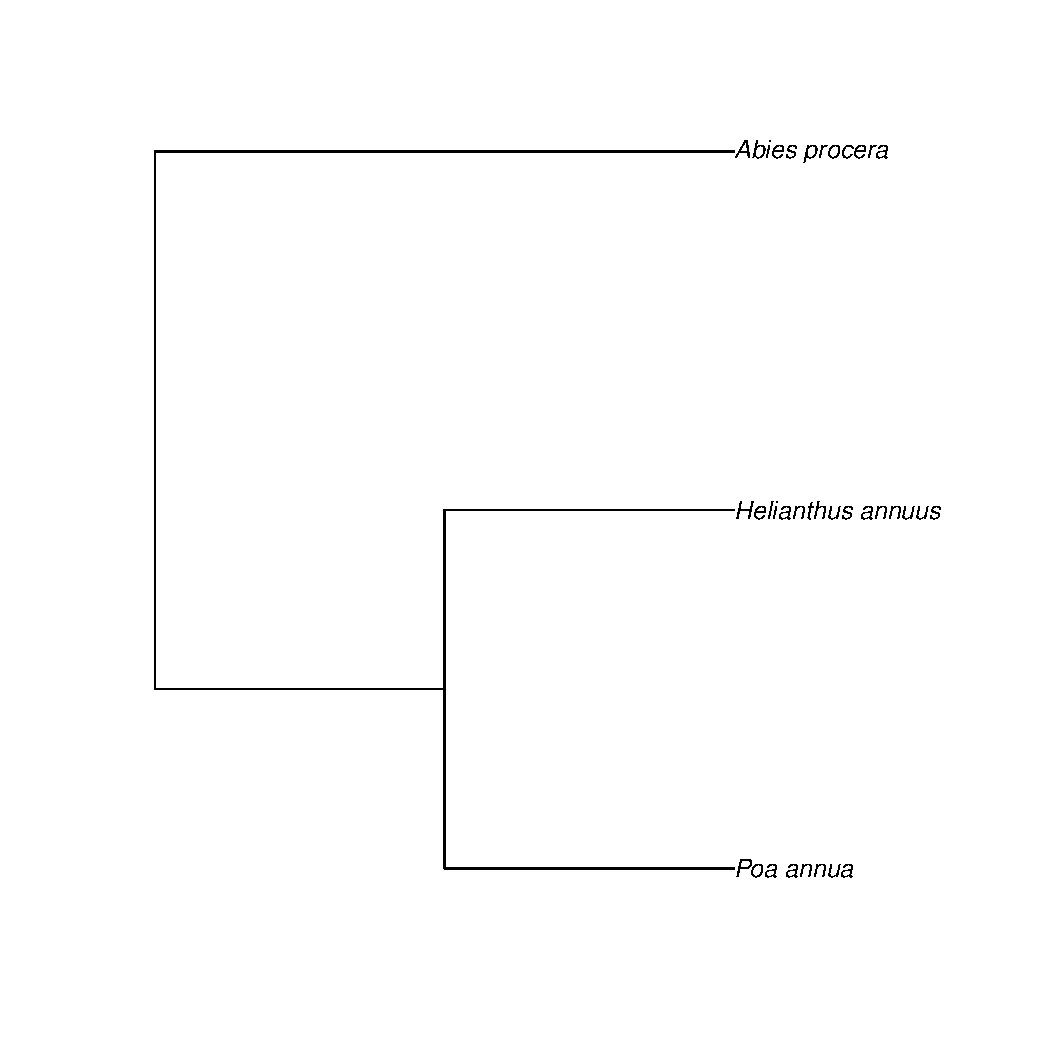
\includegraphics[width=.7\textwidth]{chapters/taxize/phylogeny.pdf}
\end{center}
\caption[A phylogeny for three species produced using the \emph{phylomatic\_tree} function.]{
{A phylogeny for three species. This phylogeny was produced using the \emph{phylomatic\_tree} function, which queries the Phylomatic database, and prunes a previously created phylogeny of plants.}
}
\label{fig:taxize:phylomatic}
\end{figure}

Behind the scenes the function \emph{phylomatic\_tree} retrieves a Taxonomic Serial Number (TSN) from ITIS for each species name, then a string is created for each species like this \emph{poaceae/oryza/oryzasativa} (with format "family/genus/\\genus\_epithet"). 
These strings are submitted to the Phylomatic API, and if no errors occur, a phylogeny in newick format is returned. 
The \emph{phylomatic\_tree()} function also cleans up the newick string and converts it to an ape \emph{phylo} object, which can be used for plotting and phylogenetic analyses. 
Be aware that Phylomatic has certain limitations - refer to the paper describing Phylomatic \citep{webb2005} and the website \url{http://phylodiversity.net/phylomatic/}.



\subsection{What taxa are children of the taxon of interest?}
If someone is not a taxonomic specialist on a particular taxon they probably do not know what children taxa are within a family, or within a genus. 
This task becomes especially unwieldy when there are a large number of taxa downstream. 
You can of course go to a website like Wikispecies (\url{http://species.wikimedia.org}) or Encyclopedia of Life (\url{http://eol.org/}) to get downstream names. 
However, taxize provides an easy way to programatically search for downstream taxa, both for the Catalogue of Life (CoL) (\url{http://www.catalogueoflife.org/}) and the Integrated Taxonomic Information System (\url{http://www.itis.gov/}). 
Here is a short example using the CoL in which we want to find all the species within the genus \emph{Apis} (honey bees).

\begin{knitrout}
\small
\definecolor{shadecolor}{rgb}{0.969, 0.969, 0.969}
\color{fgcolor}
\begin{kframe}
\begin{alltt}
\hlkwd{col_downstream}\hlstd{(}\hlkwc{name} \hlstd{=} \hlstr{"Apis"}\hlstd{,} \hlkwc{downto} \hlstd{=} \hlstr{"Species"}\hlstd{)[[}\hlnum{1}\hlstd{]]}
\end{alltt}
\begin{verbatim}
#   childtaxa_id     childtaxa_name childtaxa_rank
# 1      6971712 Apis andreniformis        Species
# 2      6971713        Apis cerana        Species
# 3      6971714       Apis dorsata        Species
# 4      6971715        Apis florea        Species
# 5      6971716 Apis koschevnikovi        Species
# 6      6845885     Apis mellifera        Species
# 7      6971717   Apis nigrocincta        Species
\end{verbatim}
\end{kframe}
\end{knitrout}

The result from the above call to \emph{col\_downstream()} is a data.frame that gives a number of columns of different information.


\subsection{IUCN Status}
There are a number of things a user can do once they have the correct taxonomic names. 
One thing a user can do is ask about the conservation status of a species (IUCN Red List of Threatened Species (\url{http://www.iucnredlist.org})). 
We have provided a set of functions, \emph{iucn\_summary} and \emph{iucn\_status}, to search for species names, and extract the status information, respectively. 
Here, you can search for the panther and lynx.

\begin{knitrout}\small
\definecolor{shadecolor}{rgb}{0.969, 0.969, 0.969}
\color{fgcolor}
\begin{kframe}
\begin{alltt}
\hlstd{ia} \hlkwb{<-} \hlkwd{iucn_summary}\hlstd{(}\hlkwd{c}\hlstd{(}\hlstr{"Panthera uncia"}\hlstd{,} \hlstr{"Lynx lynx"}\hlstd{))}
\hlkwd{iucn_status}\hlstd{(ia)}
\end{alltt}
\begin{verbatim}
# Panthera uncia      Lynx lynx 
#           "EN"           "LC"
\end{verbatim}
\end{kframe}
\end{knitrout}

It turns out that the panther has a status of endangered (EN) and the lynx has a status of least concern (LC).


\subsection{Search for available genes in GenBank}
Another use case available in taxize deals with genetic sequences. 
taxize has three functions to interact with GenBank to search for available genes \\ (\emph{get\_genes\_avail}), download genes by GenBank ID (\emph{get\_genes}), and download genes via taxonomic name search, including retrieving a congeneric if the searched taxon does not exist in the database (\emph{get\_seqs}). 
In this example, one can search for gene sequences for \emph{Umbra limi}.

\begin{knitrout}\small
\definecolor{shadecolor}{rgb}{0.969, 0.969, 0.969}
\color{fgcolor}\begin{kframe}
\begin{alltt}
\hlstd{out} \hlkwb{<-} \hlkwd{get_genes_avail}\hlstd{(}\hlkwc{taxon_name} \hlstd{=} \hlstr{"Umbra limi"}\hlstd{,}
                       \hlkwc{seqrange} \hlstd{=} \hlstr{"1:2000"}\hlstd{,}
                       \hlkwc{getrelated} \hlstd{=} \hlnum{FALSE}\hlstd{)}
\end{alltt}
\end{kframe}
\end{knitrout}


Then one can ask if 'RAG1' exists in any of the gene names.

\begin{knitrout}\small
\definecolor{shadecolor}{rgb}{0.969, 0.969, 0.969}\color{fgcolor}\begin{kframe}
\begin{alltt}
\hlstd{out[}\hlkwd{grep}\hlstd{(}\hlstr{"RAG1"}\hlstd{, out}\hlopt{$}\hlstd{genesavail,} \hlkwc{ignore.case} \hlstd{=} \hlnum{TRUE}\hlstd{),} \hlopt{-}\hlnum{3}\hlstd{]}
\end{alltt}
\begin{verbatim}
#         spused length access_num       ids
# 413 Umbra limi    732   JX190826 394772608
# 427 Umbra limi    959   AY459526  45479841
# 434 Umbra limi   1631   AY380548  38858304
\end{verbatim}
\end{kframe}
\end{knitrout}


It turns out that there are 430 different unique records found. 
However, this doesn't mean that there are 430 different genes found as the API does not provide metadata to classify genes. 
You can use regular expressions (e.g., \emph{grep}) to search for the gene of interest.


\subsection{Matching species tables with different taxonomic resolution}
Biologists often need to match different sets of data tied to species. 
For example, trait-based approaches are a promising tool in ecology \citep{statzner_can_2010}. 
One problem is that abundance data must be matched with trait databases such as the NCBI Taxonomy database \citep{usseglio-polatera_biological_2000}. 
These two data tables may contain species information on different taxonomic levels and data might have to be aggregated to a joint taxonomic level, so that the data can be merged. 
taxize can help in this data-cleaning step, providing a reproducible workflow.

A user can use the mentioned \emph{classification}-function to retrieve the taxonomic hierarchy and then search the hierarchies up- and downwards for matches. 
Here is an example to match a species (A) with names of on different taxonomic levels (B1 \& B2).

\begin{knitrout}\small
\definecolor{shadecolor}{rgb}{0.969, 0.969, 0.969}\color{fgcolor}\begin{kframe}
\begin{alltt}
\hlstd{A} \hlkwb{<-} \hlstr{"gammarus roeseli"}
\hlstd{B1} \hlkwb{<-} \hlstr{"gammarus"}
\hlstd{B2} \hlkwb{<-} \hlstr{"gammaridae"}
\hlstd{A_clas} \hlkwb{<-} \hlkwd{classification}\hlstd{(A,} \hlkwc{db} \hlstd{=} \hlstr{'ncbi'}\hlstd{)}
\hlstd{B1_clas} \hlkwb{<-} \hlkwd{classification}\hlstd{(B1,} \hlkwc{db} \hlstd{=} \hlstr{'ncbi'}\hlstd{)}
\hlstd{B2_clas} \hlkwb{<-} \hlkwd{classification}\hlstd{(B2,} \hlkwc{db} \hlstd{=} \hlstr{'ncbi'}\hlstd{)}
\hlstd{A_clas[[}\hlnum{1}\hlstd{]]}\hlopt{$}\hlstd{Rank[}\hlkwd{tolower}\hlstd{(A_clas[[}\hlnum{1}\hlstd{]]}\hlopt{$}\hlstd{ScientificName)} \hlopt \hlstd{B1]}
\end{alltt}
\begin{verbatim}
# [1] "genus"
\end{verbatim}
\begin{alltt}
\hlstd{A_clas[[}\hlnum{1}\hlstd{]]}\hlopt{$}\hlstd{Rank[}\hlkwd{tolower}\hlstd{(A_clas[[}\hlnum{1}\hlstd{]]}\hlopt{$}\hlstd{ScientificName)} \hlopt \hlstd{B2]}
\end{alltt}
\begin{verbatim}
# [1] "family"
\end{verbatim}
\end{kframe}
\end{knitrout}

If one finds a direct match (here \emph{Gammarus roeseli}), they will be lucky. 
However, Gammaridae can also be matched with \emph{Gammarus roeseli}, but on a lower taxonomic level. 
A more comprehensive and realistic example (matching a trait table with an abundance table) is given in the supplemental materials.


\subsection{Aggregating data to a specific taxonomic rank}
In biology, one can ask questions at varying taxonomic levels. 
This use case is easily handled in taxize. 
A function called \emph{tax\_agg()} will aggregate community data to a specific taxonomic level. 
In this example, one can take the data for three species and aggregate them to family level. 
Again one can specify whether they want to use data from ITIS or NCBI. 
The rows in the \emph{data.frame} are different communities.

\begin{knitrout}\small
\definecolor{shadecolor}{rgb}{0.969, 0.969, 0.969}\color{fgcolor}\begin{kframe}
\begin{alltt}
\hlkwd{data}\hlstd{(dune,} \hlkwc{package} \hlstd{=} \hlstr{'vegan'}\hlstd{)}
\hlstd{df} \hlkwb{<-} \hlstd{dune[ ,} \hlkwd{c}\hlstd{(}\hlnum{1}\hlstd{,}\hlnum{3}\hlopt{:}\hlnum{4}\hlstd{)]}
\hlkwd{colnames}\hlstd{(df)} \hlkwb{<-} \hlkwd{c}\hlstd{(}\hlstr{"Bellis perennis"}\hlstd{,} \hlstr{"Juncus bufonius"}\hlstd{,}
                  \hlstr{"Juncus articulatus"}\hlstd{)}
\hlkwd{head}\hlstd{(df)}
\end{alltt}
\begin{verbatim}
#    Bellis perennis Juncus bufonius Juncus articulatus
# 2                3               0                  0
# 13               0               3                  0
# 4                2               0                  0
# 16               0               0                  3
# 6                0               0                  0
# 1                0               0                  0
\end{verbatim}
\end{kframe}
\end{knitrout}


\begin{knitrout}footnotesize
\definecolor{shadecolor}{rgb}{0.969, 0.969, 0.969}\color{fgcolor}\begin{kframe}
\begin{alltt}
\hlstd{agg} \hlkwb{<-} \hlkwd{tax_agg}\hlstd{(df,} \hlkwc{rank} \hlstd{=} \hlstr{'family'}\hlstd{,} \hlkwc{db} \hlstd{=} \hlstr{'ncbi'}\hlstd{)}
\hlstd{agg}
\end{alltt}
\begin{verbatim}
# 
# 	Aggregated community data
# 
# Level of Aggregation: FAMILY
# No. taxa before aggregation: 3
# No. taxa after aggregation: 2
# No. taxa not found: 0
\end{verbatim}
\end{kframe}
\end{knitrout}


\begin{knitrout}\small
\definecolor{shadecolor}{rgb}{0.969, 0.969, 0.969}\color{fgcolor}\begin{kframe}
\begin{alltt}
\hlkwd{head}\hlstd{(agg}\hlopt{$}\hlstd{x)}
\end{alltt}
\begin{verbatim}
#    Asteraceae Juncaceae
# 2           3         0
# 13          0         3
# 4           2         0
# 16          0         3
# 6           0         0
# 1           0         0
\end{verbatim}
\end{kframe}
\end{knitrout}

The two \emph{Juncus} species are aggregated to the family Juncaceae and their abundances are summed. 
There was only a single species in the family Asteraceae, so the data for \emph{Bellis perennis} are carried over.


%% ----------------------------------------------------------------------------
\section{Conclusions}
\label{sec:taxize:conclusions}
Taxonomic information is increasingly sought by biologists as we take phylogenetic and taxonomic approaches to science.
Taxonomic data are becoming more widely available on the web, yet scientists require programmatic access to this data for developing reproducible workflows.
taxize was created to bridge this gap - to bring taxonomic data on the web into R, where the data can be easily manipulated, visualized, and analyzed in a reproducible workflow.

We have outlined a suite of use cases in taxize that will likely fit real use cases for many biologists.
Of course we have not thought of all possible use cases, so we hope that the biology community can give us feedback on what use cases they want to see available in taxize.
One thing we could change in the future is to make functions that fit use cases, and then allow users to select the data source as a parameter in the function.
This could possibly make the user interface easier to understand.

taxize is currently under development and will be for some time given the large number of data sources knitted together in the package, and the fact that APIs for each data source can change, requiring changes in taxize code.
Contributions to taxize are strongly encouraged, and can be easily done using GitHub here: \url{https://github.com/ropensci/taxize}.
We hope taxize will be taken up by the community and developed collaboratively, making it progressively better through time as new use cases arise, bug reports are squashed, and contributions are merged.

%% ----------------------------------------------------------------------------
\newpage
\section{References}
\printbibliography[heading=none]

\end{sloppypar}


%----------------------------------------------------------------------------
% Discussion
\cleardoublepage
\def\dir{chapters/discussion}
% -*- root: ../../thesis.tex -*-
\chapter{General Discussion}
\label{sec:discussion} 
 
\section{Statistical Ecotoxicology}


% discuss also non-detects, for examples (ritz groundwater, bienen,...)
% NOEC problem seit Jahren.


\section{Leveraging monitoring data for ecological risk assessment}



\section{Challenges to utilize 'Big Data' in ecological risk assessment}




\section{Conclusions and outlook}


% data will get more important....
% Dealing with censored data?

% ue of reach as an example
% use of censored data => e.g goulsen or ritz

%% ----------------------------------------------------------------------------
\section{References}
\printbibliography[heading=none, sorting=nyt]




\appendix

%----------------------------------------------------------------------------
% usetheglm
\cleardoublepage
\part*{Supplemental Materials}
\def\dir{appendix/usetheglm}
\chapter[Supplemental Information for: Ecotoxicology is not normal]{Supplemental Information for: Ecotoxicology is not normal - A comparison of statistical approaches for analysis of count and proportion data in ecotoxicology}
\label{ap:usetheglm}  

\section{Supplementary Tables}

\begin{table}
\centering
\caption[Count data simulations - Proportion of models converged]{Count data simulations - Proportion of models converged. N = sample sizes, 
             $\mu_C$ = mean abundance in control, LM = Linear model after transformation, 
             $GLM_{nb}$ = negative binomial model, $GLM_{qp}$ = quasi-Poisson model, 
             $GLM_{p}$ = Poisson model} 
\label{tab:conv}
{\footnotesize
\begin{tabular}{rrrrrr}
  \hline
N & $\mu_C$ & LM & $GLM_{nb}$ & $GLM_{qp}$ & $GLM_{p}$ \\ 
  \hline
3.00 & 2.00 & 1.00 & 0.33 & 1.00 & 1.00 \\ 
  3.00 & 4.00 & 1.00 & 0.53 & 1.00 & 1.00 \\ 
  3.00 & 8.00 & 1.00 & 0.79 & 1.00 & 1.00 \\ 
  3.00 & 16.00 & 1.00 & 0.94 & 1.00 & 1.00 \\ 
  3.00 & 32.00 & 1.00 & 0.99 & 1.00 & 1.00 \\ 
  3.00 & 64.00 & 1.00 & 1.00 & 1.00 & 1.00 \\ 
  3.00 & 128.00 & 1.00 & 1.00 & 1.00 & 1.00 \\ 
  6.00 & 2.00 & 1.00 & 0.63 & 1.00 & 1.00 \\ 
  6.00 & 4.00 & 1.00 & 0.85 & 1.00 & 1.00 \\ 
  6.00 & 8.00 & 1.00 & 0.98 & 1.00 & 1.00 \\ 
  6.00 & 16.00 & 1.00 & 1.00 & 1.00 & 1.00 \\ 
  6.00 & 32.00 & 1.00 & 1.00 & 1.00 & 1.00 \\ 
  6.00 & 64.00 & 1.00 & 1.00 & 1.00 & 1.00 \\ 
  6.00 & 128.00 & 1.00 & 1.00 & 1.00 & 1.00 \\ 
  9.00 & 2.00 & 1.00 & 0.76 & 1.00 & 1.00 \\ 
  9.00 & 4.00 & 1.00 & 0.95 & 1.00 & 1.00 \\ 
  9.00 & 8.00 & 1.00 & 1.00 & 1.00 & 1.00 \\ 
  9.00 & 16.00 & 1.00 & 1.00 & 1.00 & 1.00 \\ 
  9.00 & 32.00 & 1.00 & 1.00 & 1.00 & 1.00 \\ 
  9.00 & 64.00 & 1.00 & 1.00 & 1.00 & 1.00 \\ 
  9.00 & 128.00 & 1.00 & 1.00 & 1.00 & 1.00 \\ 
   \hline
\end{tabular}
}
\end{table}

% latex table generated in R 3.1.3 by xtable 1.7-4 package
% Mon Mar 23 13:00:13 2015
\begin{table}
\centering
\caption[Count data simulations - Power to detect a treatment effect.]{Count data simulations - Power to detect a treatment effect. N = sample sizes, 
             $\mu_C$ = mean abundance in control, LM = Linear model after transformation, 
             $GLM_{nb}$ = negative binomial model, $GLM_{qp}$ = quasi-Poisson model, $GLM_{qp}$ = Poisson model,
            np = pairwise Wilcoxon test.} 
\label{tab:pow_glob_c}
{\footnotesize
\begin{tabular}{rrrrrrrr}
  \hline
N & $\mu_C$ & LM & $GLM_{nb}$ & $GLM_{qp}$ & $GLM_{p}$ & np & NA \\ 
  \hline
3.00 & 2.00 & 0.13 & 0.17 & 0.17 & 0.08 & 0.36 & 0.04 \\ 
  3.00 & 4.00 & 0.14 & 0.18 & 0.17 & 0.10 & 0.54 & 0.06 \\ 
  3.00 & 8.00 & 0.19 & 0.36 & 0.24 & 0.21 & 0.78 & 0.09 \\ 
  3.00 & 16.00 & 0.23 & 0.49 & 0.33 & 0.29 & 0.95 & 0.14 \\ 
  3.00 & 32.00 & 0.31 & 0.57 & 0.38 & 0.35 & 0.99 & 0.16 \\ 
  3.00 & 64.00 & 0.32 & 0.58 & 0.38 & 0.34 & 1.00 & 0.18 \\ 
  3.00 & 128.00 & 0.35 & 0.61 & 0.42 & 0.37 & 1.00 & 0.19 \\ 
  6.00 & 2.00 & 0.26 & 0.30 & 0.29 & 0.22 & 0.49 & 0.21 \\ 
  6.00 & 4.00 & 0.36 & 0.48 & 0.44 & 0.40 & 0.78 & 0.32 \\ 
  6.00 & 8.00 & 0.48 & 0.64 & 0.57 & 0.53 & 0.94 & 0.44 \\ 
  6.00 & 16.00 & 0.59 & 0.76 & 0.70 & 0.65 & 0.99 & 0.54 \\ 
  6.00 & 32.00 & 0.68 & 0.82 & 0.76 & 0.73 & 1.00 & 0.63 \\ 
  6.00 & 64.00 & 0.72 & 0.85 & 0.80 & 0.77 & 1.00 & 0.64 \\ 
  6.00 & 128.00 & 0.73 & 0.84 & 0.80 & 0.76 & 1.00 & 0.63 \\ 
  9.00 & 2.00 & 0.34 & 0.40 & 0.42 & 0.35 & 0.64 & 0.31 \\ 
  9.00 & 4.00 & 0.56 & 0.69 & 0.66 & 0.63 & 0.91 & 0.54 \\ 
  9.00 & 8.00 & 0.70 & 0.82 & 0.79 & 0.76 & 0.98 & 0.68 \\ 
  9.00 & 16.00 & 0.81 & 0.91 & 0.89 & 0.88 & 1.00 & 0.79 \\ 
  9.00 & 32.00 & 0.89 & 0.95 & 0.94 & 0.92 & 1.00 & 0.87 \\ 
  9.00 & 64.00 & 0.92 & 0.96 & 0.95 & 0.95 & 1.00 & 0.89 \\ 
  9.00 & 128.00 & 0.94 & 0.97 & 0.96 & 0.95 & 1.00 & 0.91 \\ 
   \hline
\end{tabular}
}
\end{table}

% latex table generated in R 3.1.3 by xtable 1.7-4 package
% Mon Mar 23 13:00:23 2015
\begin{table}
\centering
\caption[Count data simulations - Power to detect LOEC.]{Count data simulations - Power to detect LOEC. N = sample sizes, 
             $\mu_C$ = mean abundance in control, LM = Linear model after transformation, 
             $GLM_{nb}$ = negative binomial model, $GLM_{qp}$ = quasi-Poisson model, 
            $GLM_{p}$ = Poisson model, np = pairwise Wilcoxon test.} 
\label{tab:pow_loec_c}
{\footnotesize
\begin{tabular}{rrrrrrr}
  \hline
N & $\mu_C$ & LM & $GLM_{nb}$ & $GLM_{qp}$ & $GLM_{p}$ & np \\ 
  \hline
3.00 & 2.00 & 0.05 & 0.01 & 0.02 & 0.02 & 0.00 \\ 
  3.00 & 4.00 & 0.08 & 0.09 & 0.08 & 0.15 & 0.00 \\ 
  3.00 & 8.00 & 0.11 & 0.22 & 0.12 & 0.30 & 0.00 \\ 
  3.00 & 16.00 & 0.13 & 0.30 & 0.18 & 0.42 & 0.00 \\ 
  3.00 & 32.00 & 0.17 & 0.35 & 0.22 & 0.50 & 0.00 \\ 
  3.00 & 64.00 & 0.19 & 0.37 & 0.23 & 0.51 & 0.00 \\ 
  3.00 & 128.00 & 0.18 & 0.37 & 0.23 & 0.53 & 0.00 \\ 
  6.00 & 2.00 & 0.14 & 0.11 & 0.09 & 0.15 & 0.06 \\ 
  6.00 & 4.00 & 0.17 & 0.23 & 0.19 & 0.30 & 0.12 \\ 
  6.00 & 8.00 & 0.28 & 0.39 & 0.32 & 0.52 & 0.20 \\ 
  6.00 & 16.00 & 0.33 & 0.48 & 0.39 & 0.59 & 0.23 \\ 
  6.00 & 32.00 & 0.40 & 0.54 & 0.47 & 0.64 & 0.28 \\ 
  6.00 & 64.00 & 0.44 & 0.56 & 0.48 & 0.61 & 0.29 \\ 
  6.00 & 128.00 & 0.44 & 0.57 & 0.49 & 0.56 & 0.29 \\ 
  9.00 & 2.00 & 0.19 & 0.20 & 0.18 & 0.26 & 0.13 \\ 
  9.00 & 4.00 & 0.29 & 0.37 & 0.31 & 0.48 & 0.27 \\ 
  9.00 & 8.00 & 0.40 & 0.52 & 0.46 & 0.62 & 0.35 \\ 
  9.00 & 16.00 & 0.51 & 0.63 & 0.57 & 0.70 & 0.45 \\ 
  9.00 & 32.00 & 0.57 & 0.69 & 0.63 & 0.68 & 0.52 \\ 
  9.00 & 64.00 & 0.61 & 0.72 & 0.66 & 0.65 & 0.53 \\ 
  9.00 & 128.00 & 0.65 & 0.73 & 0.68 & 0.61 & 0.58 \\ 
   \hline
\end{tabular}
}
\end{table}

% latex table generated in R 3.1.3 by xtable 1.7-4 package
% Mon Mar 23 13:00:16 2015
\begin{table}
\centering
\caption[Count data simulations - Type 1 error to detect a global treatment effect.]{Count data simulations - Type 1 error to detect a global treatment effect. N = sample sizes, 
             $\mu_C$ = mean abundance in control, LM = Linear model after transformation, 
             $GLM_{nb}$ = negative binomial model, $GLM_{qp}$ = quasi-Poisson model, 
             $GLM_{pb}$ = negative binomial model with parametric boostrap, 
             $GLM_{p}$ = Poisson model, np = Kruskal-Wallis test.} 
\label{tab:t1_glob_c}
{\footnotesize
\begin{tabular}{rrrrrrrr}
  \hline
N & $\mu_C$ & LM & $GLM_{nb}$ & $GLM_{qp}$ & $GLM_{pb}$ & $GLM_{p}$ & np \\ 
  \hline
3.00 & 2.00 & 0.07 & 0.04 & 0.02 & 0.07 & 0.21 & 0.03 \\ 
  3.00 & 4.00 & 0.05 & 0.07 & 0.03 & 0.05 & 0.37 & 0.01 \\ 
  3.00 & 8.00 & 0.04 & 0.12 & 0.05 & 0.05 & 0.58 & 0.02 \\ 
  3.00 & 16.00 & 0.05 & 0.14 & 0.05 & 0.05 & 0.84 & 0.02 \\ 
  3.00 & 32.00 & 0.04 & 0.13 & 0.03 & 0.04 & 0.94 & 0.01 \\ 
  3.00 & 64.00 & 0.05 & 0.16 & 0.05 & 0.05 & 0.99 & 0.03 \\ 
  3.00 & 128.00 & 0.05 & 0.13 & 0.05 & 0.06 & 1.00 & 0.02 \\ 
  6.00 & 2.00 & 0.04 & 0.05 & 0.04 & 0.06 & 0.20 & 0.03 \\ 
  6.00 & 4.00 & 0.05 & 0.08 & 0.05 & 0.05 & 0.36 & 0.04 \\ 
  6.00 & 8.00 & 0.06 & 0.09 & 0.05 & 0.06 & 0.58 & 0.04 \\ 
  6.00 & 16.00 & 0.05 & 0.08 & 0.05 & 0.05 & 0.80 & 0.04 \\ 
  6.00 & 32.00 & 0.06 & 0.08 & 0.05 & 0.06 & 0.94 & 0.04 \\ 
  6.00 & 64.00 & 0.05 & 0.09 & 0.05 & 0.05 & 0.98 & 0.04 \\ 
  6.00 & 128.00 & 0.05 & 0.09 & 0.04 & 0.05 & 1.00 & 0.04 \\ 
  9.00 & 2.00 & 0.06 & 0.06 & 0.05 & 0.07 & 0.20 & 0.05 \\ 
  9.00 & 4.00 & 0.04 & 0.08 & 0.05 & 0.06 & 0.36 & 0.04 \\ 
  9.00 & 8.00 & 0.05 & 0.08 & 0.05 & 0.06 & 0.58 & 0.04 \\ 
  9.00 & 16.00 & 0.04 & 0.07 & 0.04 & 0.05 & 0.81 & 0.04 \\ 
  9.00 & 32.00 & 0.04 & 0.06 & 0.04 & 0.06 & 0.94 & 0.05 \\ 
  9.00 & 64.00 & 0.04 & 0.07 & 0.05 & 0.05 & 0.99 & 0.04 \\ 
  9.00 & 128.00 & 0.05 & 0.07 & 0.05 & 0.06 & 1.00 & 0.04 \\ 
   \hline
\end{tabular}
}
\end{table}

% latex table generated in R 3.1.3 by xtable 1.7-4 package
% Mon Mar 23 13:00:27 2015
\begin{table}
\centering
\caption[Count data simulations - Type 1 error to detect LOEC.]{Count data simulations - Type 1 error to detect LOEC. N = sample sizes, 
             $\mu_C$ = mean abundance in control, LM = Linear model after transformation, 
             $GLM_{nb}$ = negative binomial model, $GLM_{qp}$ = quasi-Poisson model, 
            $GLM_{p}$ = Poisson model, np = pairwise Wilcoxon.} 
\label{tab:t1_loec_c}
{\footnotesize
\begin{tabular}{rrrrrrr}
  \hline
N & $\mu_C$ & LM & $GLM_{nb}$ & $GLM_{qp}$ & $GLM_{p}$ & np \\ 
  \hline
3.00 & 2.00 & 0.05 & 0.02 & 0.02 & 0.02 & 0.00 \\ 
  3.00 & 4.00 & 0.04 & 0.08 & 0.04 & 0.14 & 0.00 \\ 
  3.00 & 8.00 & 0.05 & 0.11 & 0.06 & 0.24 & 0.00 \\ 
  3.00 & 16.00 & 0.03 & 0.11 & 0.04 & 0.36 & 0.00 \\ 
  3.00 & 32.00 & 0.04 & 0.15 & 0.05 & 0.55 & 0.00 \\ 
  3.00 & 64.00 & 0.05 & 0.16 & 0.06 & 0.61 & 0.00 \\ 
  3.00 & 128.00 & 0.04 & 0.13 & 0.05 & 0.68 & 0.00 \\ 
  6.00 & 2.00 & 0.04 & 0.04 & 0.02 & 0.07 & 0.02 \\ 
  6.00 & 4.00 & 0.03 & 0.06 & 0.03 & 0.15 & 0.02 \\ 
  6.00 & 8.00 & 0.04 & 0.08 & 0.05 & 0.26 & 0.03 \\ 
  6.00 & 16.00 & 0.04 & 0.08 & 0.05 & 0.37 & 0.03 \\ 
  6.00 & 32.00 & 0.04 & 0.08 & 0.04 & 0.52 & 0.03 \\ 
  6.00 & 64.00 & 0.05 & 0.10 & 0.05 & 0.61 & 0.04 \\ 
  6.00 & 128.00 & 0.04 & 0.08 & 0.04 & 0.66 & 0.05 \\ 
  9.00 & 2.00 & 0.03 & 0.05 & 0.04 & 0.08 & 0.03 \\ 
  9.00 & 4.00 & 0.04 & 0.06 & 0.05 & 0.15 & 0.04 \\ 
  9.00 & 8.00 & 0.04 & 0.05 & 0.04 & 0.27 & 0.04 \\ 
  9.00 & 16.00 & 0.04 & 0.07 & 0.04 & 0.38 & 0.03 \\ 
  9.00 & 32.00 & 0.03 & 0.05 & 0.04 & 0.49 & 0.03 \\ 
  9.00 & 64.00 & 0.04 & 0.06 & 0.04 & 0.61 & 0.04 \\ 
  9.00 & 128.00 & 0.04 & 0.06 & 0.04 & 0.67 & 0.04 \\ 
   \hline
\end{tabular}
}
\end{table}


% latex table generated in R 3.1.3 by xtable 1.7-4 package
% Fri Mar 20 19:40:07 2015
\begin{table}
\centering
\caption[Binomial data simulations - Power to detect a global treatment effect.]{Binomial data simulations - Power to detect a global treatment effect. N = sample sizes, 
             $p_E$ = probability in effect treatments, LM = Linear model after transformation, 
             $GLM$ = binomial model, np = Kruskal-Wallis test.} 
\label{tab:pow_glob_p}
{\footnotesize
\begin{tabular}{rrrrr}
  \hline
N & $p_E$ & LM & $GLM$ & np \\ 
  \hline
3.00 & 0.60 & 0.97 & 1.00 & 0.87 \\ 
  3.00 & 0.65 & 0.90 & 0.99 & 0.76 \\ 
  3.00 & 0.70 & 0.78 & 0.95 & 0.60 \\ 
  3.00 & 0.75 & 0.60 & 0.84 & 0.41 \\ 
  3.00 & 0.80 & 0.36 & 0.64 & 0.22 \\ 
  3.00 & 0.85 & 0.20 & 0.41 & 0.10 \\ 
  3.00 & 0.90 & 0.11 & 0.17 & 0.05 \\ 
  3.00 & 0.95 & 0.06 & 0.06 & 0.03 \\ 
  6.00 & 0.60 & 1.00 & 1.00 & 1.00 \\ 
  6.00 & 0.65 & 1.00 & 1.00 & 1.00 \\ 
  6.00 & 0.70 & 1.00 & 1.00 & 1.00 \\ 
  6.00 & 0.75 & 0.97 & 1.00 & 0.97 \\ 
  6.00 & 0.80 & 0.85 & 0.93 & 0.82 \\ 
  6.00 & 0.85 & 0.53 & 0.62 & 0.48 \\ 
  6.00 & 0.90 & 0.17 & 0.24 & 0.15 \\ 
  6.00 & 0.95 & 0.04 & 0.08 & 0.03 \\ 
  9.00 & 0.60 & 1.00 & 1.00 & 1.00 \\ 
  9.00 & 0.65 & 1.00 & 1.00 & 1.00 \\ 
  9.00 & 0.70 & 1.00 & 1.00 & 1.00 \\ 
  9.00 & 0.75 & 1.00 & 1.00 & 1.00 \\ 
  9.00 & 0.80 & 0.98 & 0.99 & 0.97 \\ 
  9.00 & 0.85 & 0.75 & 0.82 & 0.73 \\ 
  9.00 & 0.90 & 0.26 & 0.32 & 0.23 \\ 
  9.00 & 0.95 & 0.05 & 0.07 & 0.04 \\ 
   \hline
\end{tabular}
}
\end{table}

% latex table generated in R 3.1.3 by xtable 1.7-4 package
% Fri Mar 20 19:40:13 2015
\begin{table}
\centering
\caption[Count data simulations - Power to detect LOEC.]{Count data simulations - Power to detect LOEC. N = sample sizes, 
             $p_E$ = probability in effect treatments, LM = Linear model after transformation, 
             $GLM$ = binomial model, np = pairwise Wilcoxon.} 
\label{tab:pow_loec_p}
{\footnotesize
\begin{tabular}{rrrrr}
  \hline
N & $p_E$ & LM & $GLM$ & np \\ 
  \hline
3.00 & 0.60 & 0.86 & 0.70 & 0.00 \\ 
  3.00 & 0.65 & 0.74 & 0.57 & 0.00 \\ 
  3.00 & 0.70 & 0.59 & 0.40 & 0.00 \\ 
  3.00 & 0.75 & 0.41 & 0.17 & 0.00 \\ 
  3.00 & 0.80 & 0.23 & 0.04 & 0.00 \\ 
  3.00 & 0.85 & 0.11 & 0.01 & 0.00 \\ 
  3.00 & 0.90 & 0.05 & 0.00 & 0.00 \\ 
  3.00 & 0.95 & 0.01 & 0.00 & 0.00 \\ 
  6.00 & 0.60 & 0.98 & 0.95 & 0.97 \\ 
  6.00 & 0.65 & 0.97 & 0.93 & 0.91 \\ 
  6.00 & 0.70 & 0.93 & 0.90 & 0.82 \\ 
  6.00 & 0.75 & 0.82 & 0.78 & 0.62 \\ 
  6.00 & 0.80 & 0.60 & 0.55 & 0.36 \\ 
  6.00 & 0.85 & 0.33 & 0.19 & 0.16 \\ 
  6.00 & 0.90 & 0.08 & 0.01 & 0.03 \\ 
  6.00 & 0.95 & 0.01 & 0.00 & 0.00 \\ 
  9.00 & 0.60 & 0.97 & 0.95 & 0.97 \\ 
  9.00 & 0.65 & 0.98 & 0.96 & 0.98 \\ 
  9.00 & 0.70 & 0.97 & 0.96 & 0.96 \\ 
  9.00 & 0.75 & 0.94 & 0.93 & 0.89 \\ 
  9.00 & 0.80 & 0.82 & 0.81 & 0.73 \\ 
  9.00 & 0.85 & 0.46 & 0.43 & 0.35 \\ 
  9.00 & 0.90 & 0.13 & 0.08 & 0.08 \\ 
  9.00 & 0.95 & 0.01 & 0.00 & 0.00 \\ 
   \hline
\end{tabular}
}
\end{table}

% latex table generated in R 3.1.3 by xtable 1.7-4 package
% Fri Mar 20 19:40:09 2015
\begin{table}
\centering
\caption[Binomial data simulations - Type 1 error to detect a global treatment effect.]{Binomial data simulations - Type 1 error to detect a global treatment effect. N = sample sizes, 
             $p$ = probability, LM = Linear model after transformation, 
             $GLM$ = binomial model, np = Kruskal-Wallis test.} 
\label{tab:t1_glob_p}
{\footnotesize
\begin{tabular}{rrrrr}
  \hline
N & $p$ & LM & $GLM$ & np \\ 
  \hline
3.00 & 0.60 & 0.05 & 0.06 & 0.02 \\ 
  3.00 & 0.65 & 0.06 & 0.06 & 0.02 \\ 
  3.00 & 0.70 & 0.04 & 0.05 & 0.02 \\ 
  3.00 & 0.75 & 0.06 & 0.05 & 0.02 \\ 
  3.00 & 0.80 & 0.05 & 0.07 & 0.02 \\ 
  3.00 & 0.85 & 0.06 & 0.07 & 0.02 \\ 
  3.00 & 0.90 & 0.05 & 0.08 & 0.01 \\ 
  3.00 & 0.95 & 0.06 & 0.07 & 0.02 \\ 
  6.00 & 0.60 & 0.06 & 0.06 & 0.04 \\ 
  6.00 & 0.65 & 0.04 & 0.05 & 0.03 \\ 
  6.00 & 0.70 & 0.04 & 0.05 & 0.04 \\ 
  6.00 & 0.75 & 0.05 & 0.05 & 0.03 \\ 
  6.00 & 0.80 & 0.06 & 0.06 & 0.04 \\ 
  6.00 & 0.85 & 0.04 & 0.06 & 0.04 \\ 
  6.00 & 0.90 & 0.06 & 0.06 & 0.04 \\ 
  6.00 & 0.95 & 0.05 & 0.08 & 0.03 \\ 
  9.00 & 0.60 & 0.05 & 0.05 & 0.04 \\ 
  9.00 & 0.65 & 0.06 & 0.06 & 0.05 \\ 
  9.00 & 0.70 & 0.06 & 0.05 & 0.05 \\ 
  9.00 & 0.75 & 0.05 & 0.05 & 0.05 \\ 
  9.00 & 0.80 & 0.06 & 0.07 & 0.06 \\ 
  9.00 & 0.85 & 0.04 & 0.05 & 0.04 \\ 
  9.00 & 0.90 & 0.06 & 0.07 & 0.05 \\ 
  9.00 & 0.95 & 0.06 & 0.06 & 0.04 \\ 
   \hline
\end{tabular}
}
\end{table}

% latex table generated in R 3.1.3 by xtable 1.7-4 package
% Fri Mar 20 19:40:15 2015
\begin{table}
\centering
\caption[Binomial data simulations - Type 1 error to detect LOEC.]{Binomial data simulations - Type 1 error to detect LOEC. N = sample sizes, 
             $p$ = probability, LM = Linear model after transformation, 
             $GLM$ = binomial model, np = pairwise Wilcoxon.} 
\label{tab:t1_loec_p}
{\footnotesize
\begin{tabular}{rrrrr}
  \hline
N & $p_E$ & LM & $GLM$ & np \\ 
  \hline
3.00 & 0.60 & 0.03 & 0.03 & 0.00 \\ 
  3.00 & 0.65 & 0.04 & 0.03 & 0.00 \\ 
  3.00 & 0.70 & 0.04 & 0.03 & 0.00 \\ 
  3.00 & 0.75 & 0.04 & 0.03 & 0.00 \\ 
  3.00 & 0.80 & 0.03 & 0.01 & 0.00 \\ 
  3.00 & 0.85 & 0.04 & 0.01 & 0.00 \\ 
  3.00 & 0.90 & 0.03 & 0.00 & 0.00 \\ 
  3.00 & 0.95 & 0.05 & 0.00 & 0.00 \\ 
  6.00 & 0.60 & 0.05 & 0.06 & 0.02 \\ 
  6.00 & 0.65 & 0.03 & 0.04 & 0.01 \\ 
  6.00 & 0.70 & 0.05 & 0.04 & 0.02 \\ 
  6.00 & 0.75 & 0.03 & 0.03 & 0.02 \\ 
  6.00 & 0.80 & 0.04 & 0.04 & 0.01 \\ 
  6.00 & 0.85 & 0.03 & 0.02 & 0.01 \\ 
  6.00 & 0.90 & 0.05 & 0.01 & 0.01 \\ 
  6.00 & 0.95 & 0.05 & 0.00 & 0.01 \\ 
  9.00 & 0.60 & 0.04 & 0.04 & 0.04 \\ 
  9.00 & 0.65 & 0.04 & 0.03 & 0.04 \\ 
  9.00 & 0.70 & 0.05 & 0.04 & 0.05 \\ 
  9.00 & 0.75 & 0.03 & 0.04 & 0.02 \\ 
  9.00 & 0.80 & 0.04 & 0.04 & 0.03 \\ 
  9.00 & 0.85 & 0.04 & 0.03 & 0.03 \\ 
  9.00 & 0.90 & 0.04 & 0.03 & 0.03 \\ 
  9.00 & 0.95 & 0.05 & 0.00 & 0.01 \\ 
   \hline
\end{tabular}
}
\end{table}


\FloatBarrier

\section{Worked R examples}
% -*- root: ../../../thesis.tex -*-

\subsection{Count data example}
\subsubsection{Introduction}
In this example we will analyse data from \citep{brock_minimum_2015}.
The data are count of mayfly larvae in Macroinvertebrate Artificial Substrate Samplers in 18 mesocosms at one sampling day.
There are 5 treatments and one control group.

First, we load the data, bring it to the long format and remove NA values.
\begin{knitrout}
\color{fgcolor}\small\begin{kframe}
\begin{alltt}
\hlstd{R> df} \hlkwb{<-} \hlkwd{read.table}\hlstd{(}\hlkwc{header} \hlstd{=} \hlnum{TRUE}\hlstd{,}
                 \hlkwc{text} \hlstd{=} \hlstr{'Control  T0.1 T0.3  T1  T3  T10
                          175 29  27  36  26  20
                          65  114 78  11  13  37
                          154 72  27  105 33  NA
                          83  NA  NA  NA  NA  NA'}\hlstd{)}
\hlstd{R> }\hlkwd{require}\hlstd{(reshape2)}
\hlstd{R> dfm} \hlkwb{<-} \hlkwd{melt}\hlstd{(df,} \hlkwc{value.name} \hlstd{=} \hlstr{'abu'}\hlstd{,} \hlkwc{variable.name} \hlstd{=} \hlstr{'treatment'}\hlstd{)}
\hlstd{R> dfm} \hlkwb{<-} \hlstd{dfm[}\hlopt{!}\hlkwd{is.na}\hlstd{(dfm[}\hlstr{'abu'}\hlstd{]), ]}
\hlstd{R> }\hlkwd{head}\hlstd{(dfm)}
\end{alltt}
\begin{verbatim}
##   treatment abu
## 1   Control 175
## 2   Control  65
## 3   Control 154
## 4   Control  83
## 5      T0.1  29
## 6      T0.1 114
\end{verbatim}
\end{kframe}
\end{knitrout}
This results in a table with two columns - one indicating the treatment and one with the measured abundances.

  
Let's have a first look at the data:
\begin{knitrout}
\color{fgcolor}\small\begin{kframe}
\begin{alltt}
\hlstd{R> }\hlkwd{boxplot}\hlstd{(abu} \hlopt{~} \hlstd{treatment,} \hlkwc{data} \hlstd{= dfm,} \hlkwc{xlab} \hlstd{=} \hlstr{'Treatment'}\hlstd{,}
            \hlkwc{ylab} \hlstd{=} \hlstr{'Count'}\hlstd{,} \hlkwc{col} \hlstd{=} \hlstr{'grey75'}\hlstd{,} \hlkwc{main} \hlstd{=} \hlstr{'Raw abundances'}\hlstd{)}
\end{alltt}
\end{kframe}

{\centering 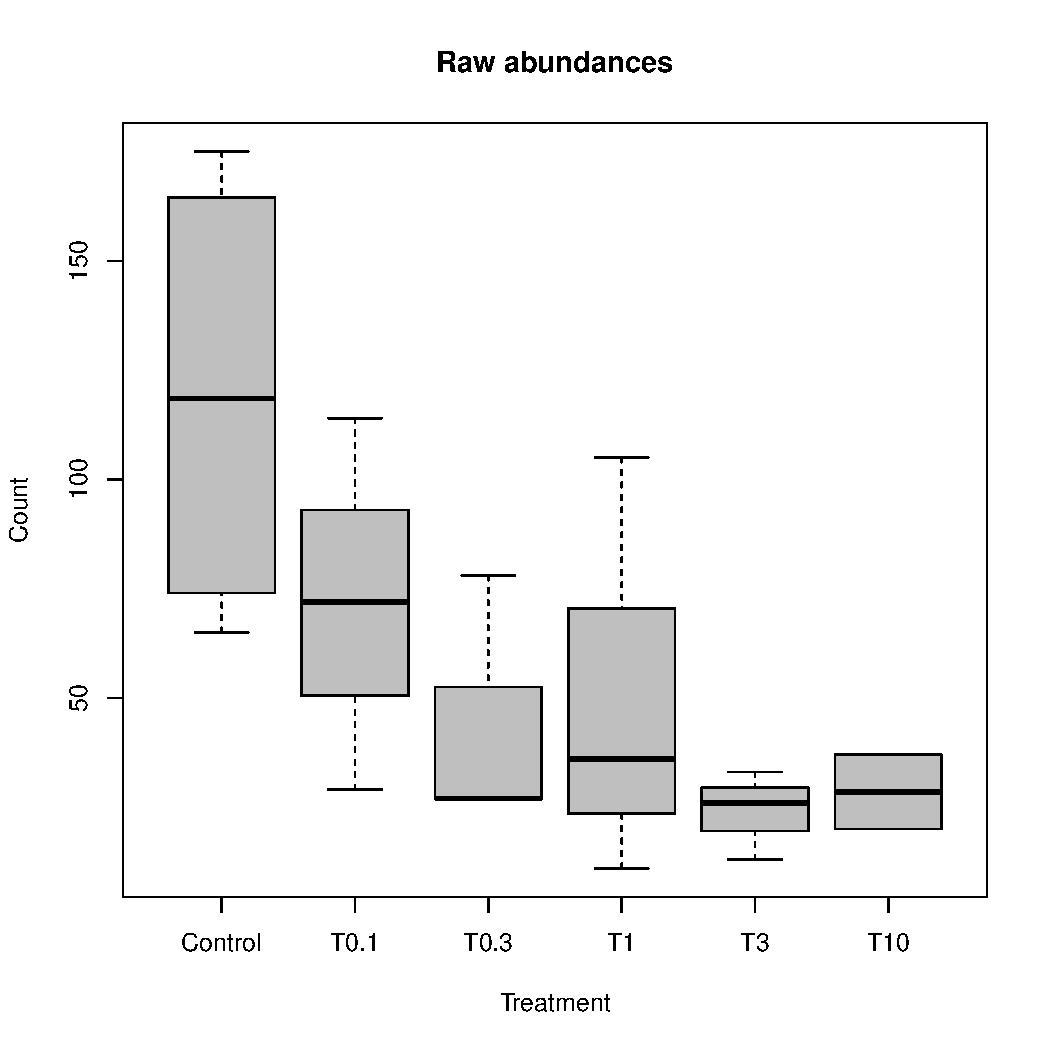
\includegraphics[width=0.8\textwidth]{appendix/usetheglm/two/count_raw_plot-1} 

}



\end{knitrout}
We clearly see a treatment related response. 
Moreover, we may note that variances are increasing with increasing abundances.



\subsubsection{Assuming a normal distribution of transformed abundances}
\subsubsection{Data transformation}
Next we transform the data using a ln(Ax + 1) transformation.
A is chosen so that the term Ax equals two for the lowest non-zero abundance.
We add these transformed abundances as extra column to our table.

\begin{knitrout}
\color{fgcolor}\small\begin{kframe}
\begin{alltt}
\hlstd{R> A} \hlkwb{<-} \hlnum{2} \hlopt{/} \hlkwd{min}\hlstd{(dfm}\hlopt{$}\hlstd{abu[dfm}\hlopt{$}\hlstd{abu} \hlopt{!=} \hlnum{0}\hlstd{])}
\hlstd{R> A}
\end{alltt}
\begin{verbatim}
## [1] 0.1818182
\end{verbatim}
\begin{alltt}
\hlstd{R> dfm}\hlopt{$}\hlstd{abu_t} \hlkwb{<-} \hlkwd{log}\hlstd{(A} \hlopt{*} \hlstd{dfm}\hlopt{$}\hlstd{abu} \hlopt{+} \hlnum{1}\hlstd{)}
\hlstd{R> }\hlkwd{head}\hlstd{(dfm)}
\end{alltt}
\begin{verbatim}
##   treatment abu    abu_t
## 1   Control 175 3.490983
## 2   Control  65 2.550865
## 3   Control 154 3.367296
## 4   Control  83 2.778254
## 5      T0.1  29 1.836211
## 6      T0.1 114 3.078568
\end{verbatim}
\end{kframe}
\end{knitrout}


It looks like the transformation does a good job in equalizing the variances:
\begin{knitrout}
\color{fgcolor}\small\begin{kframe}
\begin{alltt}
\hlstd{R> }\hlkwd{boxplot}\hlstd{(abu_t} \hlopt{~} \hlstd{treatment,} \hlkwc{data} \hlstd{= dfm,}
            \hlkwc{xlab} \hlstd{=} \hlstr{'Treatment'}\hlstd{,} \hlkwc{ylab} \hlstd{=} \hlstr{'Transf. Counts'}\hlstd{,}
            \hlkwc{col} \hlstd{=} \hlstr{'grey75'}\hlstd{,} \hlkwc{main} \hlstd{=} \hlstr{'Transformed abundances'}\hlstd{)}
\end{alltt}
\end{kframe}

{\centering 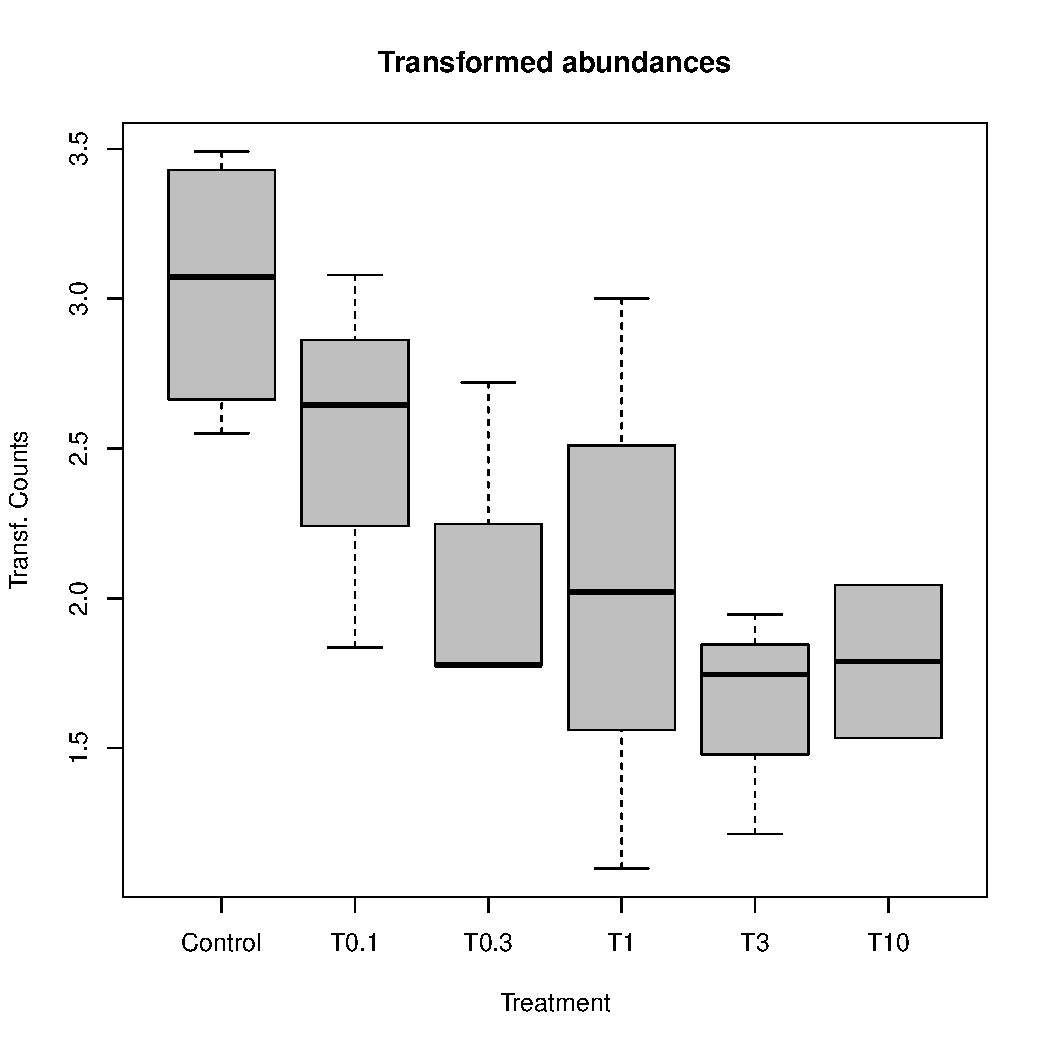
\includegraphics[width=0.8\textwidth]{appendix/usetheglm/two/plot_count_trans-1} 

}



\end{knitrout}


\subsubsection{Model fitting}
The model from eqn. 2 can be easily fitted using the \texttt{lm()} function:

\begin{knitrout}
\color{fgcolor}\small\begin{kframe}
\begin{alltt}
\hlstd{R> modlm} \hlkwb{<-} \hlkwd{lm}\hlstd{(abu_t} \hlopt{~} \hlstd{treatment,} \hlkwc{data} \hlstd{= dfm)}
\end{alltt}
\end{kframe}
\end{knitrout}

The residuals vs. fitted values diagnostic plot show no problematic pattern, though it might be difficult to decide with such a small sample size
\begin{knitrout}
\color{fgcolor}\small\begin{kframe}
\begin{alltt}
\hlstd{R> }\hlkwd{plot}\hlstd{(}\hlkwd{residuals}\hlstd{(modlm)} \hlopt{~} \hlkwd{fitted}\hlstd{(modlm))}
\hlstd{R> }\hlkwd{abline}\hlstd{(}\hlkwc{h} \hlstd{=} \hlnum{0}\hlstd{,} \hlkwc{lty} \hlstd{=} \hlstr{'dotted'}\hlstd{)}
\end{alltt}
\end{kframe}

{\centering 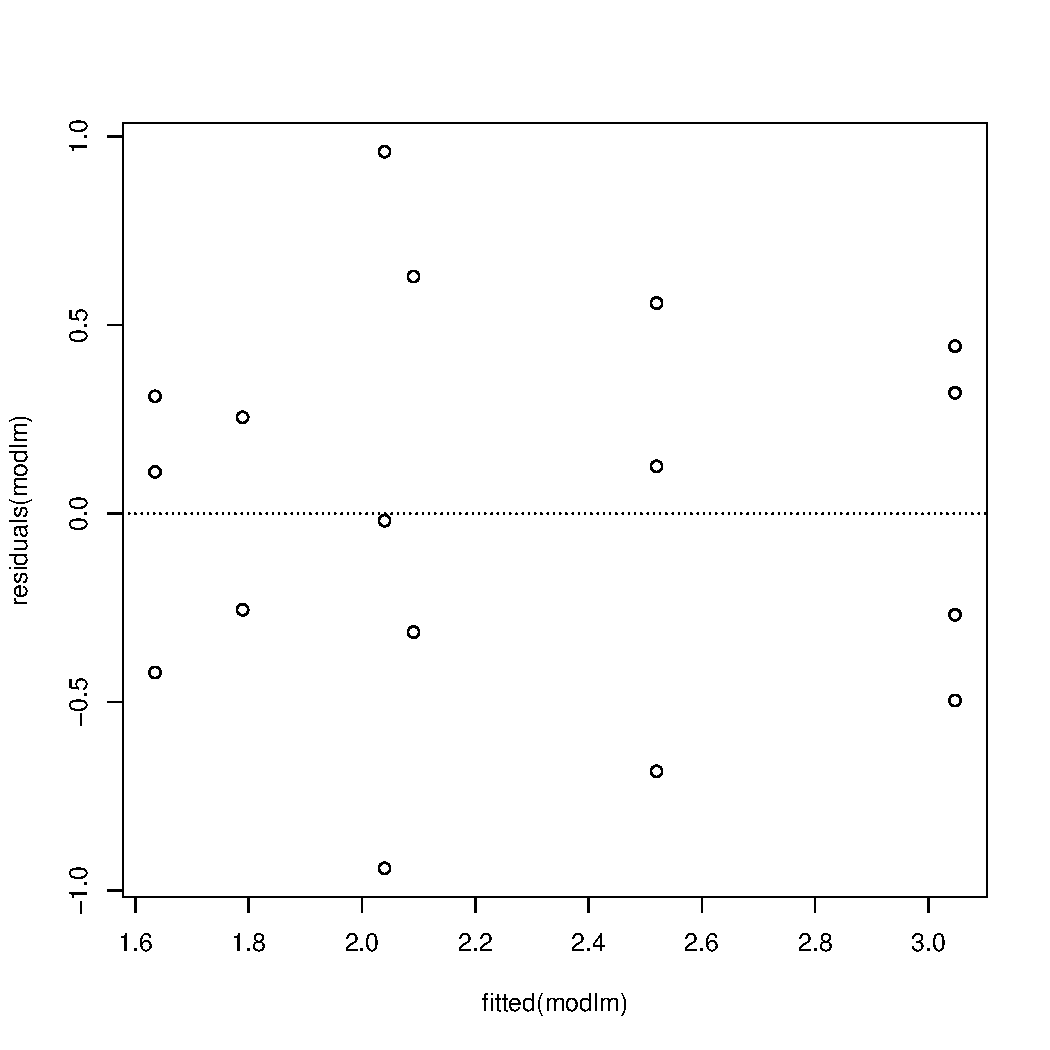
\includegraphics[width=0.8\textwidth]{appendix/usetheglm/two/plot_modlm-1} 

}



\end{knitrout}

The \texttt{summary()} gives the estimated coefficients with standard errors and Wald t tests:
\begin{knitrout}
\color{fgcolor}\small\begin{kframe}
\begin{alltt}
\hlstd{R> }\hlkwd{summary}\hlstd{(modlm)}
\end{alltt}
\begin{verbatim}
## 
## Call:
## lm(formula = abu_t ~ treatment, data = dfm)
## 
## Residuals:
##      Min       1Q   Median       3Q      Max 
## -0.94133 -0.31454  0.04576  0.31813  0.96033 
## 
## Coefficients:
##               Estimate Std. Error t value Pr(>|t|)    
## (Intercept)     3.0468     0.2970  10.260 2.71e-07 ***
## treatmentT0.1  -0.5267     0.4536  -1.161  0.26814    
## treatmentT0.3  -0.9558     0.4536  -2.107  0.05682 .  
## treatmentT1    -1.0069     0.4536  -2.220  0.04646 *  
## treatmentT3    -1.4121     0.4536  -3.113  0.00897 ** 
## treatmentT10   -1.2575     0.5144  -2.445  0.03089 *  
## ---
## Signif. codes:  0 '***' 0.001 '**' 0.01 '*' 0.05 '.' 0.1 ' ' 1
## 
## Residual standard error: 0.5939 on 12 degrees of freedom
## Multiple R-squared:  0.5167,	Adjusted R-squared:  0.3154 
## F-statistic: 2.566 on 5 and 12 DF,  p-value: 0.08406
\end{verbatim}
\end{kframe}
\end{knitrout}

\subsubsection{Inference on general treatment effect}
Or, if you want to have the ANOVA table with an F-test:
\begin{knitrout}
\color{fgcolor}\small\begin{kframe}
\begin{alltt}
\hlstd{R> }\hlkwd{summary.aov}\hlstd{(modlm)}
\end{alltt}
\begin{verbatim}
##             Df Sum Sq Mean Sq F value Pr(>F)  
## treatment    5  4.526  0.9052   2.566 0.0841 .
## Residuals   12  4.233  0.3528                 
## ---
## Signif. codes:  0 '***' 0.001 '**' 0.01 '*' 0.05 '.' 0.1 ' ' 1
\end{verbatim}
\end{kframe}
\end{knitrout}

From this output we might infer that we cannot detect any treatment effect (F = 2.566, p = 0.084).

\subsubsection{Inference on LOEC}
Let's move on to the LOEC determination.
This can be easily done using the multcomp package \citep{hothorn_simultaneous_2008}:

Here we perform a one-sided (\texttt{alternative = 'less'}) using Dunnett contrasts of treatment (\texttt{mcp(treatment='Dunnett')}).
Moreover, we adjust for multiple testing using Holm's method (\texttt{test = adjusted('holm')}):
\begin{knitrout}
\color{fgcolor}\small\begin{kframe}
\begin{alltt}
\hlstd{R> }\hlkwd{require}\hlstd{(multcomp)}
\hlstd{R> }\hlkwd{summary}\hlstd{(}\hlkwd{glht}\hlstd{(modlm,} \hlkwc{linfct} \hlstd{=} \hlkwd{mcp}\hlstd{(}\hlkwc{treatment} \hlstd{=} \hlstr{'Dunnett'}\hlstd{),}  
                \hlkwc{alternative} \hlstd{=} \hlstr{'less'}\hlstd{),}
                \hlkwc{test} \hlstd{=} \hlkwd{adjusted}\hlstd{(}\hlstr{'holm'}\hlstd{))}
\end{alltt}
\begin{verbatim}
## 
## 	 Simultaneous Tests for General Linear Hypotheses
## 
## Multiple Comparisons of Means: Dunnett Contrasts
## 
## 
## Fit: lm(formula = abu_t ~ treatment, data = dfm)
## 
## Linear Hypotheses:
##                     Estimate Std. Error t value Pr(<t)  
## T0.1 - Control >= 0  -0.5267     0.4536  -1.161 0.1341  
## T0.3 - Control >= 0  -0.9558     0.4536  -2.107 0.0697 .
## T1 - Control >= 0    -1.0069     0.4536  -2.220 0.0697 .
## T3 - Control >= 0    -1.4121     0.4536  -3.113 0.0224 *
## T10 - Control >= 0   -1.2575     0.5144  -2.445 0.0618 .
## ---
## Signif. codes:  0 '***' 0.001 '**' 0.01 '*' 0.05 '.' 0.1 ' ' 1
## (Adjusted p values reported -- holm method)
\end{verbatim}
\end{kframe}
\end{knitrout}

Here only treatment 3 mg/L shows a statistically significant difference from control and is the determined LOEC.
The column \texttt{'Estimate'} gives the estimated difference in means between treatments and control and \texttt{'Std. Error'} the standard errors of these estimates.


To determine the LOEC we could also use a Williams type contrast  \citep{bretz_multiple_2010}. 

Here I use a step-up Williams contrast.
First we need to define a contrast matrix (see also \texttt{?contrMat()}):

\begin{knitrout}
\color{fgcolor}\small\begin{kframe}
\begin{alltt}
\hlcom{# observations per treatment}
\hlstd{R> n} \hlkwb{<-} \hlkwd{tapply}\hlstd{(dfm}\hlopt{$}\hlstd{abu_t, dfm}\hlopt{$}\hlstd{treatment, length)}
\hlstd{R> k} \hlkwb{<-} \hlkwd{length}\hlstd{(n)}
\hlstd{R> CM} \hlkwb{<-} \hlkwd{c}\hlstd{()}
\hlstd{R> }\hlkwa{for} \hlstd{(i} \hlkwa{in} \hlnum{1}\hlopt{:}\hlstd{(k} \hlopt{-} \hlnum{1}\hlstd{)) \{}
      \hlstd{help} \hlkwb{<-} \hlkwd{c}\hlstd{(}\hlopt{-}\hlnum{1}\hlstd{, n[}\hlnum{2}\hlopt{:}\hlstd{(i} \hlopt{+} \hlnum{1}\hlstd{)]} \hlopt{/} \hlkwd{sum}\hlstd{(n[}\hlnum{2}\hlopt{:}\hlstd{(i} \hlopt{+} \hlnum{1}\hlstd{)]),} \hlkwd{rep}\hlstd{(}\hlnum{0} \hlstd{, k} \hlopt{-} \hlstd{i} \hlopt{-} \hlnum{1}\hlstd{))}
      \hlstd{CM} \hlkwb{<-} \hlkwd{rbind}\hlstd{(CM, help)}
\hlstd{\}}
\hlstd{R> }\hlkwd{rownames}\hlstd{(CM)} \hlkwb{<-} \hlkwd{paste}\hlstd{(}\hlstr{"C"}\hlstd{,} \hlnum{1}\hlopt{:}\hlkwd{nrow}\hlstd{(CM))}
\hlstd{R> CM}
\end{alltt}
\begin{verbatim}
##             T0.1                                        
## C 1 -1 1.0000000 0.0000000 0.0000000 0.0000000 0.0000000
## C 2 -1 0.5000000 0.5000000 0.0000000 0.0000000 0.0000000
## C 3 -1 0.3333333 0.3333333 0.3333333 0.0000000 0.0000000
## C 4 -1 0.2500000 0.2500000 0.2500000 0.2500000 0.0000000
## C 5 -1 0.2142857 0.2142857 0.2142857 0.2142857 0.1428571
\end{verbatim}
\end{kframe}
\end{knitrout}

Then we supply this contrast matrix to \texttt{glht()}:
\begin{knitrout}
\color{fgcolor}\small\begin{kframe}
\begin{alltt}
\hlstd{R> }\hlkwd{summary}\hlstd{(}\hlkwd{glht}\hlstd{(modlm,} \hlkwc{linfct} \hlstd{=} \hlkwd{mcp}\hlstd{(}\hlkwc{treatment} \hlstd{= CM),}
                \hlkwc{alternative} \hlstd{=} \hlstr{'less'}\hlstd{),}
                \hlkwc{test} \hlstd{=} \hlkwd{adjusted}\hlstd{(}\hlstr{'holm'}\hlstd{))}
\end{alltt}
\begin{verbatim}
## 
## 	 Simultaneous Tests for General Linear Hypotheses
## 
## Multiple Comparisons of Means: User-defined Contrasts
## 
## 
## Fit: lm(formula = abu_t ~ treatment, data = dfm)
## 
## Linear Hypotheses:
##          Estimate Std. Error t value Pr(<t)  
## C 1 >= 0  -0.5267     0.4536  -1.161 0.1341  
## C 2 >= 0  -0.7413     0.3834  -1.934 0.0771 .
## C 3 >= 0  -0.8298     0.3569  -2.325 0.0576 .
## C 4 >= 0  -0.9754     0.3429  -2.845 0.0295 *
## C 5 >= 0  -1.0157     0.3367  -3.016 0.0268 *
## ---
## Signif. codes:  0 '***' 0.001 '**' 0.01 '*' 0.05 '.' 0.1 ' ' 1
## (Adjusted p values reported -- holm method)
\end{verbatim}
\end{kframe}
\end{knitrout}

This indicates a LOEC at 3 mg/L.

If we do not adjust for multiple testing (\texttt{test = adjusted('none')}), we end up with the same NOEC  (0.1 mg/L) as \citet{brock_minimum_2015}:
\begin{knitrout}
\color{fgcolor}\small\begin{kframe}
\begin{alltt}
\hlstd{R> }\hlkwd{summary}\hlstd{(}\hlkwd{glht}\hlstd{(modlm,} \hlkwc{linfct} \hlstd{=} \hlkwd{mcp}\hlstd{(}\hlkwc{treatment} \hlstd{= CM),}
                \hlkwc{alternative} \hlstd{=} \hlstr{'less'}\hlstd{),}
                \hlkwc{test} \hlstd{=} \hlkwd{adjusted}\hlstd{(}\hlstr{'none'}\hlstd{))}
\end{alltt}
\begin{verbatim}
## 
## 	 Simultaneous Tests for General Linear Hypotheses
## 
## Multiple Comparisons of Means: User-defined Contrasts
## 
## 
## Fit: lm(formula = abu_t ~ treatment, data = dfm)
## 
## Linear Hypotheses:
##          Estimate Std. Error t value  Pr(<t)   
## C 1 >= 0  -0.5267     0.4536  -1.161 0.13407   
## C 2 >= 0  -0.7413     0.3834  -1.934 0.03855 * 
## C 3 >= 0  -0.8298     0.3569  -2.325 0.01921 * 
## C 4 >= 0  -0.9754     0.3429  -2.845 0.00739 **
## C 5 >= 0  -1.0157     0.3367  -3.016 0.00537 **
## ---
## Signif. codes:  0 '***' 0.001 '**' 0.01 '*' 0.05 '.' 0.1 ' ' 1
## (Adjusted p values reported -- none method)
\end{verbatim}
\end{kframe}
\end{knitrout}

Note, this multiple contrast test is different from the original Williams test \citep{williams_comparison_1972} used by \citep{brock_minimum_2015}. See \citet{bretz_powerful_1999} for a comparison.




\subsubsection{Assuming a Poisson distribution of abundances}
\subsubsection{Model fitting}
We are dealing with count data, so a Poisson GLM might be a good choice.
GLMs can be fitted using the \texttt{glm()} function and here we fit the model from eqn. 3:
\begin{knitrout}
\color{fgcolor}\small\begin{kframe}
\begin{alltt}
\hlstd{R> modpois} \hlkwb{<-} \hlkwd{glm}\hlstd{(abu} \hlopt{~} \hlstd{treatment,} \hlkwc{data} \hlstd{= dfm,} 
                  \hlkwc{family} \hlstd{=} \hlkwd{poisson}\hlstd{(}\hlkwc{link} \hlstd{=} \hlstr{'log'}\hlstd{))}
\end{alltt}
\end{kframe}
\end{knitrout}

Here \texttt{family = poisson(link = 'log')} specifies that we want to fit a poisson model using a log link between response and predictors.

The \texttt{summary} gives the estimated coefficients, standard errors and Wald Z tests:
\begin{knitrout}
\color{fgcolor}\small\begin{kframe}
\begin{alltt}
\hlstd{R> (sum_pois} \hlkwb{<-} \hlkwd{summary}\hlstd{(modpois))}
\end{alltt}
\begin{verbatim}
## 
## Call:
## glm(formula = abu ~ treatment, family = poisson(link = "log"), 
##     data = dfm)
## 
## Deviance Residuals: 
##     Min       1Q   Median       3Q      Max  
## -6.7625  -2.7621  -0.8219   2.7172   6.6602  
## 
## Coefficients:
##               Estimate Std. Error z value Pr(>|z|)    
## (Intercept)    4.78122    0.04579 104.423  < 2e-16 ***
## treatmentT0.1 -0.50920    0.08214  -6.199 5.69e-10 ***
## treatmentT0.3 -0.99703    0.09835 -10.138  < 2e-16 ***
## treatmentT1   -0.85595    0.09314  -9.190  < 2e-16 ***
## treatmentT3   -1.60317    0.12643 -12.680  < 2e-16 ***
## treatmentT10  -1.43132    0.14014 -10.213  < 2e-16 ***
## ---
## Signif. codes:  0 '***' 0.001 '**' 0.01 '*' 0.05 '.' 0.1 ' ' 1
## 
## (Dispersion parameter for poisson family taken to be 1)
## 
##     Null deviance: 604.79  on 17  degrees of freedom
## Residual deviance: 273.77  on 12  degrees of freedom
## AIC: 387.63
## 
## Number of Fisher Scoring iterations: 5
\end{verbatim}
\end{kframe}
\end{knitrout}


But is a poisson distribution appropriate here? 
A property of the poisson distribution is that its variance is equal to the mean. 
A simple diagnostic would be to plot group variances vs. group means:

\begin{knitrout}
\color{fgcolor}\small\begin{kframe}
\begin{alltt}
\hlstd{R> }\hlkwd{require}\hlstd{(plyr)}
\hlcom{# mean and variance per treatment}
\hlstd{R> musd} \hlkwb{<-} \hlkwd{ddply}\hlstd{(dfm,} \hlkwd{.}\hlstd{(treatment), summarise,}
                 \hlkwc{mu} \hlstd{=} \hlkwd{mean}\hlstd{(abu),}
                 \hlkwc{var} \hlstd{=} \hlkwd{var}\hlstd{(abu))}
\hlstd{R> musd}
\end{alltt}
\begin{verbatim}
##   treatment        mu      var
## 1   Control 119.25000 2857.583
## 2      T0.1  71.66667 1806.333
## 3      T0.3  44.00000  867.000
## 4        T1  50.66667 2370.333
## 5        T3  24.00000  103.000
## 6       T10  28.50000  144.500
\end{verbatim}
\begin{alltt}
\hlcom{# plot mean vs var}
\hlstd{R> }\hlkwd{plot}\hlstd{(var} \hlopt{~} \hlstd{mu,} \hlkwc{data} \hlstd{= musd,}
        \hlkwc{xlab} \hlstd{=} \hlstr{'mean'}\hlstd{,} \hlkwc{ylab} \hlstd{=} \hlstr{'variance'}\hlstd{,} 
        \hlkwc{main} \hlstd{=} \hlstr{'Mean-variance relationships'}\hlstd{)}
\hlcom{# poisson}
\hlstd{R> }\hlkwd{abline}\hlstd{(}\hlkwc{a} \hlstd{=} \hlnum{0}\hlstd{,} \hlkwc{b} \hlstd{=} \hlnum{1}\hlstd{,} \hlkwc{col} \hlstd{=} \hlstr{'darkblue'}\hlstd{,} \hlkwc{lwd} \hlstd{=} \hlnum{2}\hlstd{)}
\hlcom{# quasi-Poisson}
\hlstd{R> }\hlkwd{abline}\hlstd{(}\hlkwc{a} \hlstd{=} \hlnum{0}\hlstd{,} \hlkwc{b} \hlstd{=} \hlnum{22.41}\hlstd{,} \hlkwc{col} \hlstd{=} \hlstr{'darkgreen'}\hlstd{,} \hlkwc{lwd} \hlstd{=} \hlnum{2}\hlstd{)}
\hlcom{# negative binomial}
\hlstd{R> }\hlkwd{curve}\hlstd{(x} \hlopt{+} \hlstd{(x}\hlopt{^}\hlnum{2} \hlopt{/} \hlnum{3.91}\hlstd{),} \hlkwc{from} \hlstd{=} \hlnum{24}\hlstd{,} \hlkwc{to} \hlstd{=} \hlnum{119.25}\hlstd{,} \hlkwc{add} \hlstd{=} \hlnum{TRUE}\hlstd{,}
          \hlkwc{col} \hlstd{=} \hlstr{'darkred'}\hlstd{,} \hlkwc{lwd} \hlstd{=} \hlnum{2}\hlstd{)}
\hlstd{R> }\hlkwd{legend}\hlstd{(}\hlstr{'topleft'}\hlstd{,}
          \hlkwc{legend} \hlstd{=} \hlkwd{c}\hlstd{(}\hlstr{'NB(k = 3.91)'}\hlstd{,}\hlstr{'Poisson'}\hlstd{,}\hlstr{'Quasi-Poisson(t=22.4)'}\hlstd{),}
          \hlkwc{col} \hlstd{=} \hlkwd{c}\hlstd{(}\hlstr{'darkred'}\hlstd{,} \hlstr{'darkblue'}\hlstd{,} \hlstr{'darkgreen'}\hlstd{),}
           \hlkwc{lty} \hlstd{=} \hlkwd{c}\hlstd{(}\hlnum{1}\hlstd{,}\hlnum{1}\hlstd{,} \hlnum{1}\hlstd{),}
           \hlkwc{lwd} \hlstd{=} \hlkwd{c}\hlstd{(}\hlnum{2}\hlstd{,}\hlnum{2}\hlstd{,} \hlnum{2}\hlstd{))}
\end{alltt}
\end{kframe}

{\centering 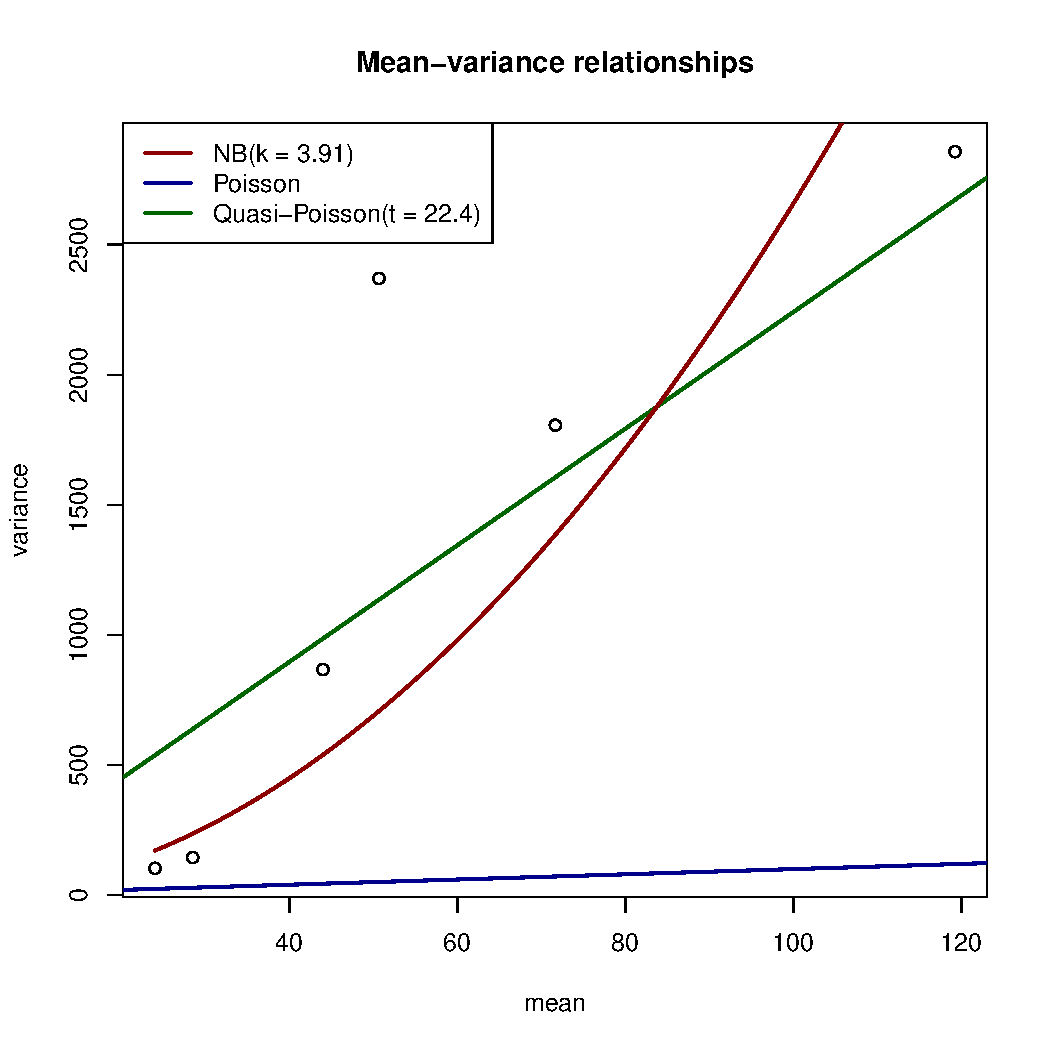
\includegraphics[width=0.8\textwidth]{appendix/usetheglm/two/mod_count_meanvar-1} 

}



\end{knitrout}

I also added the assumed mean-variance relationships of the Poisson, quasi-Poisson and negative binomial models (see below).
We clearly see that the variance increases much more than would be expected under the poisson distribution (the data is overdispersed).
Moreover, we could check overdispersion from the \texttt{summary}:
If the ratio of residual deviance to degrees of freedom is \textgreater 1 the data is overdispersed.
\begin{knitrout}
\color{fgcolor}\small\begin{kframe}
\begin{alltt}
\hlstd{R> sum_pois}\hlopt{$}\hlstd{deviance} \hlopt{/} \hlstd{sum_pois}\hlopt{$}\hlstd{df.residual}
\end{alltt}
\begin{verbatim}
## [1] 22.81412
\end{verbatim}
\end{kframe}
\end{knitrout}




\subsubsection{Apply quasi-Poisson to deal with overdispersion}
The plot above suggests that the variance may increasing stronger than the mean and a quasi-Poisson or negative binomial model might be more appropriate for this data.

\subsubsection{Model fitting}
Fitting a quasi-Poisson model (eqn. 4) is straight forward:
\begin{knitrout}
\color{fgcolor}\small\begin{kframe}
\begin{alltt}
\hlstd{R> modqpois} \hlkwb{<-} \hlkwd{glm}\hlstd{(abu} \hlopt{~} \hlstd{treatment,} \hlkwc{data} \hlstd{= dfm,} \hlkwc{family} \hlstd{=} \hlstr{'quasipoisson'}\hlstd{)}
\end{alltt}
\end{kframe}
\end{knitrout}

The summary gives the estimated coefficients:
\begin{knitrout}
\color{fgcolor}\small\begin{kframe}
\begin{alltt}
\hlstd{R> }\hlkwd{summary}\hlstd{(modqpois)}
\end{alltt}
\begin{verbatim}
## 
## Call:
## glm(formula = abu ~ treatment, family = "quasipoisson", 
##      data = dfm)
## 
## Deviance Residuals: 
##     Min       1Q   Median       3Q      Max  
## -6.7625  -2.7621  -0.8219   2.7172   6.6602  
## 
## Coefficients:
##               Estimate Std. Error t value Pr(>|t|)    
## (Intercept)     4.7812     0.2168  22.058 4.43e-11 ***
## treatmentT0.1  -0.5092     0.3889  -1.309   0.2149    
## treatmentT0.3  -0.9970     0.4656  -2.142   0.0534 .  
## treatmentT1    -0.8560     0.4409  -1.941   0.0761 .  
## treatmentT3    -1.6032     0.5985  -2.679   0.0201 *  
## treatmentT10   -1.4313     0.6634  -2.157   0.0519 .  
## ---
## Signif. codes:  0 '***' 0.001 '**' 0.01 '*' 0.05 '.' 0.1 ' ' 1
## 
## (Dispersion parameter for quasipoisson family taken to be 22.411)
## 
##     Null deviance: 604.79  on 17  degrees of freedom
## Residual deviance: 273.77  on 12  degrees of freedom
## AIC: NA
## 
## Number of Fisher Scoring iterations: 5
\end{verbatim}
\end{kframe}
\end{knitrout}

, with the dispersion parameter $\Theta = 22.41055$. 
Note, that the coefficients estimates are the same as from the Poisson model, only the standard errors are scaled/wider.

\subsubsection{Inference on general treatment effect}
An F-test can be performed using \texttt{drop1()}:
\begin{knitrout}
\color{fgcolor}\small\begin{kframe}
\begin{alltt}
\hlstd{R> }\hlkwd{drop1}\hlstd{(modqpois,} \hlkwc{test} \hlstd{=} \hlstr{'F'}\hlstd{)}
\end{alltt}
\begin{verbatim}
## Single term deletions
## 
## Model:
## abu ~ treatment
##           Df Deviance F value  Pr(>F)  
## <none>         273.77                  
## treatment  5   604.79  2.9019 0.06059 .
## ---
## Signif. codes:  0 '***' 0.001 '**' 0.01 '*' 0.05 '.' 0.1 ' ' 1
\end{verbatim}
\end{kframe}
\end{knitrout}
Here we would reject that there is treatment effect (at alpha = 0.05).

\subsubsection{Inference on LOEC}
The LOEC can be determined with \texttt{multcomp}:
\begin{knitrout}
\color{fgcolor}\small\begin{kframe}
\begin{alltt}
\hlstd{R> }\hlkwd{summary}\hlstd{(}\hlkwd{glht}\hlstd{(modqpois,} \hlkwc{linfct} \hlstd{=} \hlkwd{mcp}\hlstd{(}\hlkwc{treatment} \hlstd{=} \hlstr{'Dunnett'}\hlstd{),}
                \hlkwc{alternative} \hlstd{=} \hlstr{'less'}\hlstd{),}
                \hlkwc{test} \hlstd{=} \hlkwd{adjusted}\hlstd{(}\hlstr{'holm'}\hlstd{))}
\end{alltt}
\begin{verbatim}
## 
## 	 Simultaneous Tests for General Linear Hypotheses
## 
## Multiple Comparisons of Means: Dunnett Contrasts
## 
## 
## Fit: glm(formula = abu ~ treatment, family = "quasipoisson", 
##          data = dfm)
## 
## Linear Hypotheses:
##                     Estimate Std. Error z value Pr(<z)  
## T0.1 - Control >= 0  -0.5092     0.3889  -1.309 0.0952 .
## T0.3 - Control >= 0  -0.9970     0.4656  -2.142 0.0619 .
## T1 - Control >= 0    -0.8560     0.4409  -1.941 0.0619 .
## T3 - Control >= 0    -1.6032     0.5985  -2.679 0.0185 *
## T10 - Control >= 0   -1.4313     0.6634  -2.157 0.0619 .
## ---
## Signif. codes:  0 '***' 0.001 '**' 0.01 '*' 0.05 '.' 0.1 ' ' 1
## (Adjusted p values reported -- holm method)
\end{verbatim}
\end{kframe}
\end{knitrout}
, which determines 3 mg/L as LOEC.


\subsubsection{Assuming a negative binomial distribution of abundances}
\subsubsection{Model fitting}
To fit a negative binomial GLM (eqn. 5) we could use \texttt{glm.nb()} from the MASS package \citep{venables_modern_2002}:
\begin{knitrout}
\color{fgcolor}\small\begin{kframe}
\begin{alltt}
\hlstd{R> }\hlkwd{require}\hlstd{(MASS)}
\hlstd{R> modnb} \hlkwb{<-} \hlkwd{glm.nb}\hlstd{(abu} \hlopt{~} \hlstd{treatment,} \hlkwc{data} \hlstd{= dfm)}
\end{alltt}
\end{kframe}
\end{knitrout}

The estimated coefficients:
\begin{knitrout}
\color{fgcolor}\small\begin{kframe}
\begin{alltt}
\hlstd{R> }\hlkwd{summary}\hlstd{(modnb)}
\end{alltt}
\begin{verbatim}
## 
## Call:
## glm.nb(formula = abu ~ treatment, data = dfm, 
##     init.theta = 3.905898474, 
##     link = log)
## 
## Deviance Residuals: 
##     Min       1Q   Median       3Q      Max  
## -2.2554  -0.8488  -0.3020   0.5954   1.5899  
## 
## Coefficients:
##               Estimate Std. Error z value Pr(>|z|)    
## (Intercept)     4.7812     0.2571  18.596  < 2e-16 ***
## treatmentT0.1  -0.5092     0.3951  -1.289  0.19746    
## treatmentT0.3  -0.9970     0.3988  -2.500  0.01241 *  
## treatmentT1    -0.8560     0.3975  -2.153  0.03130 *  
## treatmentT3    -1.6032     0.4066  -3.943 8.05e-05 ***
## treatmentT10   -1.4313     0.4601  -3.111  0.00186 ** 
## ---
## Signif. codes:  0 '***' 0.001 '**' 0.01 '*' 0.05 '.' 0.1 ' ' 1
## 
## (Dispersion parameter for Negative Binomial(3.9059) 
##    family taken to be 1)
## 
##     Null deviance: 39.057  on 17  degrees of freedom
## Residual deviance: 18.611  on 12  degrees of freedom
## AIC: 181.24
## 
## Number of Fisher Scoring iterations: 1
## 
## 
##               Theta:  3.91 
##           Std. Err.:  1.37 
## 
##  2 x log-likelihood:  -167.238
\end{verbatim}
\end{kframe}
\end{knitrout}
, with $\kappa = 3.91$.


\subsubsection{Inference on general treatment effect (LR-test)}
For an LR-Test we need to first fit a reduced model:
\begin{knitrout}
\color{fgcolor}\small\begin{kframe}
\begin{alltt}
\hlstd{R> modnb.null} \hlkwb{<-} \hlkwd{glm.nb}\hlstd{(abu} \hlopt{~} \hlnum{1}\hlstd{,} \hlkwc{data} \hlstd{= dfm)}
\end{alltt}
\end{kframe}
\end{knitrout}

, so that the dispersion parameter $\kappa$ is re-estimated for the reduced model.
Then we can compare these two models with a LR-Test:
\begin{knitrout}
\color{fgcolor}\small\begin{kframe}
\begin{alltt}
\hlstd{R> }\hlkwd{anova}\hlstd{(modnb, modnb.null,} \hlkwc{test} \hlstd{=} \hlstr{'Chisq'}\hlstd{)}
\end{alltt}
\begin{verbatim}
## Likelihood ratio tests of Negative Binomial Models
## 
## Response: abu
##       Model    theta Resid. df    2 x log-lik.   Test df LR stat.
## 1         1 1.861577        17       -181.2281                      
## 2 treatment 3.905898        12       -167.2383 1 vs 2  5 13.98985
##    Pr(Chi)
## 1         
## 2 0.015674
\end{verbatim}
\end{kframe}
\end{knitrout}
, which suggests a treatment related effect on abundances.


\subsubsection{Inference on general treatment effect (parametric bootstrap)}

To test the LR statistic using paramtric bootstrap, we use two custom functions:

The first function \texttt{myPBrefdist} generates a boostrap sample and return the LR statistic for this sample:
\begin{knitrout}
\color{fgcolor}\small\begin{kframe}
\begin{alltt}
\hlcom{#' PB of LR statistic}
\hlcom{#' @param m1 Full model}
\hlcom{#' @param m0 reduced model}
\hlcom{#' @param  data data used in the models}
\hlcom{#' @return LR of boostrap}
\hlcom{# generate reference distribution}
\hlstd{R> myPBrefdist} \hlkwb{<-} \hlkwa{function}\hlstd{(}\hlkwc{m1}\hlstd{,} \hlkwc{m0}\hlstd{,} \hlkwc{data}\hlstd{)\{}
      \hlcom{# simulate from null}
      \hlstd{x0} \hlkwb{<-} \hlkwd{simulate}\hlstd{(m0)}
      \hlcom{# refit with new data}
      \hlstd{newdata0} \hlkwb{<-} \hlstd{data}
      \hlstd{newdata0[ ,} \hlkwd{as.character}\hlstd{(}\hlkwd{formula}\hlstd{(m0)[[}\hlnum{2}\hlstd{]])]} \hlkwb{<-} \hlstd{x0}
      \hlstd{m1r} \hlkwb{<-}  \hlkwd{try}\hlstd{(}\hlkwd{update}\hlstd{(m1, .}\hlopt{~}\hlstd{.,} \hlkwc{data} \hlstd{= newdata0),} \hlkwc{silent} \hlstd{=} \hlnum{TRUE}\hlstd{)}
      \hlstd{m0r} \hlkwb{<-} \hlkwd{try}\hlstd{(}\hlkwd{update}\hlstd{(m0, .}\hlopt{~}\hlstd{.,} \hlkwc{data} \hlstd{= newdata0),} \hlkwc{silent} \hlstd{=} \hlnum{TRUE}\hlstd{)}
      \hlcom{# check convergence (otherwise return NA for LR)}
      \hlkwa{if}\hlstd{(}\hlkwd{inherits}\hlstd{(m0r,} \hlstr{"try-error"}\hlstd{)} \hlopt{|} \hlkwd{inherits}\hlstd{(m1r,} \hlstr{"try-error"}\hlstd{))\{}
        \hlstd{LR} \hlkwb{<-} \hlstr{'convergence error'}
      \hlstd{\}} \hlkwa{else} \hlstd{\{}
        \hlkwa{if}\hlstd{(}\hlopt{!}\hlkwd{is.null}\hlstd{(m0r[[}\hlstr{'th.warn'}\hlstd{]])} \hlopt{| !}\hlkwd{is.null}\hlstd{(m1r[[}\hlstr{'th.warn'}\hlstd{]]))\{}
          \hlstd{LR} \hlkwb{<-} \hlstr{'convergence error'}
        \hlstd{\}} \hlkwa{else} \hlstd{\{}
          \hlstd{LR} \hlkwb{<-} \hlopt{-}\hlnum{2} \hlopt{*} \hlstd{(}\hlkwd{logLik}\hlstd{(m0r)} \hlopt{-} \hlkwd{logLik}\hlstd{(m1r))}
        \hlstd{\}}
      \hlstd{\}}
      \hlkwd{return}\hlstd{(LR)}
\hlstd{\}}
\end{alltt}
\end{kframe}
\end{knitrout}

The second one (\texttt{myPBmodcomp}) repeats \texttt{myPBrefdist} many time and returns a p-value:
\begin{knitrout}
\color{fgcolor}\small\begin{kframe}
\begin{alltt}
\hlcom{#' generate LR distribution and return p value}
\hlcom{#' @param m1 Full model}
\hlcom{#' @param m0 reduced model}
\hlcom{#' @param data data used in m1 and m0}
\hlcom{#' @param npb number of bootstrap samples}
\hlcom{#' @return p-value of boostrapped LR values}
\hlstd{R> myPBmodcomp} \hlkwb{<-} \hlkwa{function}\hlstd{(}\hlkwc{m1}\hlstd{,} \hlkwc{m0}\hlstd{,} \hlkwc{data}\hlstd{,} \hlkwc{npb}\hlstd{)\{}
      \hlcom{## calculate reference distribution}
      \hlstd{LR} \hlkwb{<-} \hlkwd{replicate}\hlstd{(npb,} \hlkwd{myPBrefdist}\hlstd{(}\hlkwc{m1} \hlstd{= m1,} \hlkwc{m0} \hlstd{= m0,} \hlkwc{data} \hlstd{= data),}
                      \hlkwc{simplify} \hlstd{=} \hlnum{TRUE}\hlstd{)}
      \hlstd{LR} \hlkwb{<-} \hlkwd{as.numeric}\hlstd{(LR)}
      \hlstd{nconv_LR} \hlkwb{<-} \hlkwd{sum}\hlstd{(}\hlopt{!}\hlkwd{is.na}\hlstd{(LR))}
      \hlcom{## original stats}
      \hlstd{LRo} \hlkwb{<-} \hlkwd{c}\hlstd{(}\hlopt{-}\hlnum{2} \hlopt{*} \hlstd{(}\hlkwd{logLik}\hlstd{(m0)} \hlopt{-} \hlkwd{logLik}\hlstd{(m1)))}
      \hlcom{## p-value from parametric bootstrap}
      \hlstd{p.pb} \hlkwb{<-} \hlkwd{mean}\hlstd{(}\hlkwd{c}\hlstd{(LR, LRo)} \hlopt{>=} \hlstd{LRo,} \hlkwc{na.rm} \hlstd{=} \hlnum{TRUE}\hlstd{)}
      \hlkwd{return}\hlstd{(}\hlkwd{list}\hlstd{(}\hlkwc{nconv_LR} \hlstd{= nconv_LR,} \hlkwc{p.pb} \hlstd{= p.pb))}
\hlstd{\}}
\end{alltt}
\end{kframe}
\end{knitrout}


Sounds complicated, but we can easily apply this to the negativ binomial model using:
\begin{knitrout}
\color{fgcolor}\small\begin{kframe}
\begin{alltt}
\hlstd{R> }\hlkwd{set.seed}\hlstd{(}\hlnum{1234}\hlstd{)}
\hlstd{R> }\hlkwd{myPBmodcomp}\hlstd{(modnb, modnb.null,} \hlkwc{data} \hlstd{= dfm,} \hlkwc{npb} \hlstd{=} \hlnum{500}\hlstd{)}
\end{alltt}
\begin{verbatim}
## $nconv_LR
## [1] 499
## 
## $p.pb
## [1] 0.042
\end{verbatim}
\end{kframe}
\end{knitrout}
Here, we specify to generate 500 bootstrap samples (\texttt{npb = 500}).
Of these 500 samples, 499 converged (\texttt{nconv\_LR}) (one did not and throws some errors) and gives a p-value of 0.042.



\subsubsection{Inference on LOEC}
This is similar to the other parametric models:
\begin{knitrout}
\color{fgcolor}\small\begin{kframe}
\begin{alltt}
\hlstd{R> }\hlkwd{summary}\hlstd{(}\hlkwd{glht}\hlstd{(modnb,} \hlkwc{linfct} \hlstd{=} \hlkwd{mcp}\hlstd{(}\hlkwc{treatment} \hlstd{=} \hlstr{'Dunnett'}\hlstd{),}  
            \hlkwc{alternative} \hlstd{=} \hlstr{'less'}\hlstd{),}
            \hlkwc{test} \hlstd{=} \hlkwd{adjusted}\hlstd{(}\hlstr{'holm'}\hlstd{))}
\end{alltt}
\begin{verbatim}
## 
## 	 Simultaneous Tests for General Linear Hypotheses
## 
## Multiple Comparisons of Means: Dunnett Contrasts
## 
## 
## Fit: glm.nb(formula = abu ~ treatment, data = dfm, 
##     init.theta = 3.905898474, 
##     link = log)
## 
## Linear Hypotheses:
##                     Estimate Std. Error z value   Pr(<z)    
## T0.1 - Control >= 0  -0.5092     0.3951  -1.289 0.098731 .  
## T0.3 - Control >= 0  -0.9970     0.3988  -2.500 0.018615 *  
## T1 - Control >= 0    -0.8560     0.3975  -2.153 0.031300 *  
## T3 - Control >= 0    -1.6032     0.4066  -3.943 0.000201 ***
## T10 - Control >= 0   -1.4313     0.4601  -3.111 0.003727 ** 
## ---
## Signif. codes:  0 '***' 0.001 '**' 0.01 '*' 0.05 '.' 0.1 ' ' 1
## (Adjusted p values reported -- holm method)
\end{verbatim}
\end{kframe}
\end{knitrout}
which suggests a LOEC at the 0.3 mg/l treatment.


\subsubsection{Non-parametric methods}
\subsubsection{Kruskal-Wallis Test}
We can use the Kruskal-Wallies test to check if there is a difference between treatments:

\begin{knitrout}
\color{fgcolor}\small\begin{kframe}
\begin{alltt}
\hlstd{R> }\hlkwd{kruskal.test}\hlstd{(abu} \hlopt{~} \hlstd{treatment,} \hlkwc{data} \hlstd{= dfm)}
\end{alltt}
\begin{verbatim}
## 
## 	Kruskal-Wallis rank sum test
## 
## data:  abu by treatment
## Kruskal-Wallis chi-squared = 8.219, df = 5, p-value = 0.1446
\end{verbatim}
\end{kframe}
\end{knitrout}

\subsubsection{Pairwise Wilcoxon test}
To determine the LOEC we could use a Pairwise Wilcoxon test.
The built-in \linebreak \texttt{pairwise.wilcox.test()} compares by default all levels (Tukey-contrasts).
We are only interested in a subset of these comparisons (Dunnett-contrast).
Therefore, we use a custom function, which is a wrapper around \texttt{wilcox.exact} from the exactRankTests package:

\begin{knitrout}
\color{fgcolor}\small\begin{kframe}
\begin{alltt}
\hlcom{#' pairwise wilcox.test with dunnett contrasrs}
\hlcom{#' @param y numeric; vector of data values}
\hlcom{#' @param g factor; grouping vector}
\hlcom{#' @param dunnett logical; if TRUE dunnett contrast, otherwise 
Tukey-contrasts}
\hlcom{#' @param padj character; method for p-adjustment, see ?p.adjust.}
\hlcom{#' @param ... other arguments passed to exactRankTests::wilcox.exact}
\hlstd{R> pairwise_wilcox} \hlkwb{<-} \hlkwa{function}\hlstd{(}\hlkwc{y}\hlstd{,} \hlkwc{g}\hlstd{,} \hlkwc{dunnett} \hlstd{=} \hlnum{TRUE}\hlstd{,} \hlkwc{padj}\hlstd{=}\hlstr{'holm'}\hlstd{,}\hlkwc{...}\hlstd{)\{}
      \hlkwa{if}\hlstd{(}\hlopt{!}\hlkwd{require}\hlstd{(exactRankTests))\{}
        \hlkwd{stop}\hlstd{(}\hlstr{'Install exactRankTests package'}\hlstd{)}
      \hlstd{\}}
      \hlstd{tc} \hlkwb{<-} \hlkwd{t}\hlstd{(}\hlkwd{combn}\hlstd{(}\hlkwd{nlevels}\hlstd{(g),} \hlnum{2}\hlstd{))}
      \hlcom{# take only dunnett comparisons}
      \hlkwa{if}\hlstd{(dunnett)\{}
        \hlstd{tc} \hlkwb{<-} \hlstd{tc[tc[ ,} \hlnum{1}\hlstd{]} \hlopt{==} \hlnum{1}\hlstd{, ]}
      \hlstd{\}}
      \hlstd{pval} \hlkwb{<-} \hlkwd{numeric}\hlstd{(}\hlkwd{nrow}\hlstd{(tc))}
      \hlcom{# use wilcox.exact (for tied data)}
      \hlkwa{for}\hlstd{(i} \hlkwa{in} \hlkwd{seq_len}\hlstd{(}\hlkwd{nrow}\hlstd{(tc)))\{}
        \hlstd{pval[i]} \hlkwb{<-} \hlkwd{wilcox.exact}\hlstd{(y[}\hlkwd{as.numeric}\hlstd{(g)} \hlopt{==} \hlstd{tc[i,} \hlnum{2}\hlstd{]],}
                                \hlstd{y[}\hlkwd{as.numeric}\hlstd{(g)} \hlopt{==} \hlstd{tc[i,} \hlnum{1}\hlstd{]],}\hlkwc{exact}\hlstd{=}\hlnum{TRUE}\hlstd{,}
                                \hlstd{...)}\hlopt{$}\hlstd{p.value}
      \hlstd{\}}

      \hlcom{# adjust p-values}
      \hlstd{pval} \hlkwb{<-} \hlkwd{p.adjust}\hlstd{(pval, padj)}
      \hlkwd{names}\hlstd{(pval)} \hlkwb{=} \hlkwd{paste}\hlstd{(}\hlkwd{levels}\hlstd{(g)[tc[,}\hlnum{1}\hlstd{]],} \hlkwd{levels}\hlstd{(g)[tc[,}\hlnum{2}\hlstd{]],} 
                \hlkwc{sep} \hlstd{=} \hlstr{' vs. '}\hlstd{)}
      \hlkwd{return}\hlstd{(pval)}
\hlstd{\}}
\end{alltt}
\end{kframe}
\end{knitrout}

Here, we use one-sided Dunnett contrasts and adjust p-values using Holm's method:
\begin{knitrout}
\color{fgcolor}\small\begin{kframe}
\begin{alltt}
\hlstd{R> }\hlkwd{pairwise_wilcox}\hlstd{(}\hlkwc{y} \hlstd{= dfm}\hlopt{$}\hlstd{abu,} \hlkwc{g} \hlstd{= dfm}\hlopt{$}\hlstd{treatment,}
                    \hlkwc{dunnett} \hlstd{=} \hlnum{TRUE}\hlstd{,} \hlkwc{p.adj} \hlstd{=} \hlstr{'holm'}\hlstd{,} \hlkwc{alternative} \hlstd{=} \hlstr{'less'}\hlstd{)}
\end{alltt}
\begin{verbatim}
## Control vs. T0.1 Control vs. T0.3  Control vs. T1  Control vs. T3 
##        0.2285714        0.2285714       0.2285714       0.1428571 
##  Control vs. T10 
##        0.2285714
\end{verbatim}
\end{kframe}
\end{knitrout}
This indicates no treatment effect at no level of concentration.




\subsection{Binomial data example}
\subsubsection{Introduction}
Here we will show how to analyse binomial data (\emph{x out of n}). 
Data is provided in \citet{newman_quantitative_2012} (example 5.1, page 223) and \citet{epa_methods_2002}.
Ten fathead minnow (\textit{Pimephales promelas}) larvals were exposed to sodium pentachlorophenol (NaPCP) and proportions of the total number alive at the end of the exposure reported.

First we load the data:
\begin{knitrout}
\color{fgcolor}\small\begin{kframe}
\begin{alltt}
\hlstd{R> df} \hlkwb{<-} \hlkwd{read.table}\hlstd{(}\hlkwc{header} \hlstd{=} \hlnum{TRUE}\hlstd{,} \hlkwc{text} \hlstd{=} \hlstr{'conc A B C D
0 1 1 0.9 0.9
32 0.8 0.8 1 0.8
64 0.9 1 1 1 
128 0.9 0.9 0.8 1
256 0.7 0.9 1 0.5
512 0.4 0.3 0.4 0.2'}\hlstd{)}
\hlstd{R> df}
\end{alltt}
\begin{verbatim}
##   conc   A   B   C   D
## 1    0 1.0 1.0 0.9 0.9
## 2   32 0.8 0.8 1.0 0.8
## 3   64 0.9 1.0 1.0 1.0
## 4  128 0.9 0.9 0.8 1.0
## 5  256 0.7 0.9 1.0 0.5
## 6  512 0.4 0.3 0.4 0.2
\end{verbatim}
\end{kframe}
\end{knitrout}

The we do some house-keeping, reformat the data and convert concentration to a factor:

\begin{knitrout}
\color{fgcolor}\small\begin{kframe}
\begin{alltt}
\hlstd{R> }\hlkwd{require}\hlstd{(reshape2)}
\hlcom{# wide to long}
\hlstd{R> dfm} \hlkwb{<-} \hlkwd{melt}\hlstd{(df,} \hlkwc{id.vars} \hlstd{=} \hlstr{'conc'}\hlstd{,} \hlkwc{value.name} \hlstd{=} \hlstr{'y'}\hlstd{,} 
                \hlkwc{variable.name} \hlstd{=} \hlstr{'tank'}\hlstd{)}
\hlcom{# conc as factor}
\hlstd{R> dfm}\hlopt{$}\hlstd{conc} \hlkwb{<-} \hlkwd{factor}\hlstd{(dfm}\hlopt{$}\hlstd{conc)}
\end{alltt}
\end{kframe}
\end{knitrout}

So after data cleaning the data looks like
\begin{knitrout}
\color{fgcolor}\small\begin{kframe}
\begin{alltt}
\hlstd{R> }\hlkwd{head}\hlstd{(dfm)}
\end{alltt}
\begin{verbatim}
##   conc tank   y
## 1    0    A 1.0
## 2   32    A 0.8
## 3   64    A 0.9
## 4  128    A 0.9
## 5  256    A 0.7
## 6  512    A 0.4
\end{verbatim}
\end{kframe}
\end{knitrout}

Let's have a first look at the data:
\begin{knitrout}
\color{fgcolor}\small\begin{kframe}
\begin{alltt}
\hlstd{R> }\hlkwd{boxplot}\hlstd{(y} \hlopt{~} \hlstd{conc,} \hlkwc{data} \hlstd{= dfm,}
            \hlkwc{xlab} \hlstd{=} \hlstr{'Concentration'}\hlstd{,} \hlkwc{ylab} \hlstd{=} \hlstr{'Proportion surv.'}\hlstd{,}
            \hlkwc{main} \hlstd{=} \hlstr{'Raw data'}\hlstd{,} \hlkwc{col} \hlstd{=} \hlstr{'grey75'}\hlstd{)}
\end{alltt}
\end{kframe}

{\centering 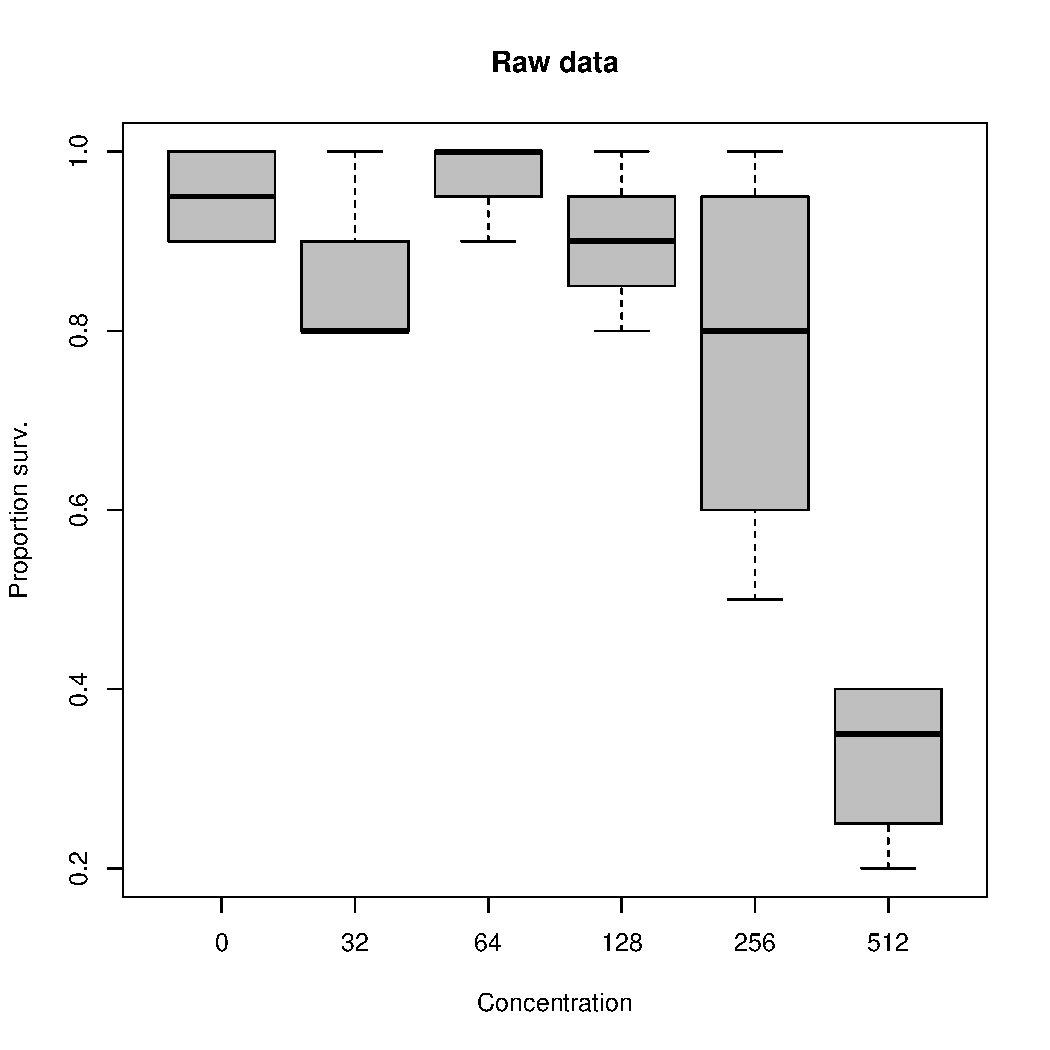
\includegraphics[width=0.8\textwidth]{appendix/usetheglm/two/bin_raw_plot-1} 

}



\end{knitrout}
This plot indicates a strong effect at the highest concentration.


\subsubsection{Assuming a normal distribution of transformed proportions}
First, we arcsine transform (eqn. 6) the proportions:
\begin{knitrout}
\color{fgcolor}\small\begin{kframe}
\begin{alltt}
\hlstd{R> dfm}\hlopt{$}\hlstd{y_asin} \hlkwb{<-} \hlkwd{ifelse}\hlstd{(dfm}\hlopt{$}\hlstd{y} \hlopt{==} \hlnum{1}\hlstd{,}
                     \hlkwd{asin}\hlstd{(}\hlnum{1}\hlstd{)} \hlopt{-} \hlkwd{asin}\hlstd{(}\hlkwd{sqrt}\hlstd{(}\hlnum{1}\hlopt{/}\hlnum{40}\hlstd{)),}
                     \hlkwd{ifelse}\hlstd{(dfm}\hlopt{$}\hlstd{y} \hlopt{==} \hlnum{0}\hlstd{,}
                            \hlkwd{asin}\hlstd{(}\hlkwd{sqrt}\hlstd{(}\hlnum{1}\hlopt{/}\hlnum{40}\hlstd{)),}
                            \hlkwd{asin}\hlstd{(}\hlkwd{sqrt}\hlstd{(dfm}\hlopt{$}\hlstd{y))}
                            \hlstd{)}
                     \hlstd{)}
\end{alltt}
\end{kframe}
\end{knitrout}

\begin{knitrout}
\color{fgcolor}\small\begin{kframe}
\begin{alltt}
\hlstd{R> }\hlkwd{boxplot}\hlstd{(y_asin} \hlopt{~} \hlstd{conc,} \hlkwc{data} \hlstd{= dfm,}
            \hlkwc{xlab} \hlstd{=} \hlstr{'Concentration'}\hlstd{,} \hlkwc{ylab} \hlstd{=} \hlstr{'Proportion surv.'}\hlstd{,}
            \hlkwc{main} \hlstd{=} \hlstr{'Transformed data'}\hlstd{,} \hlkwc{col} \hlstd{=} \hlstr{'grey75'}\hlstd{)}
\end{alltt}
\end{kframe}

{\centering 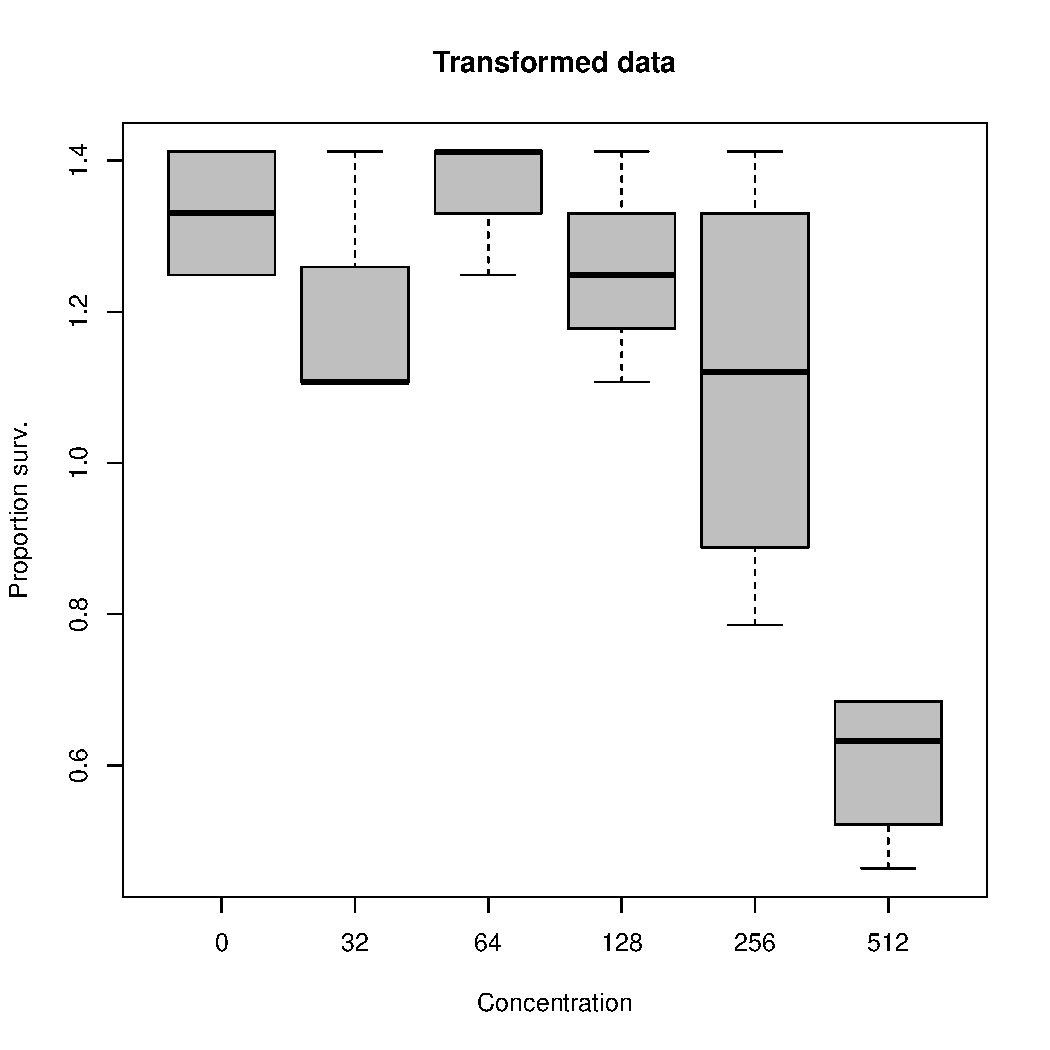
\includegraphics[width=0.8\textwidth]{appendix/usetheglm/two/bin_trans_plot-1} 

}



\end{knitrout}


Then, like in the count data example we fit the model using \texttt{lm()}:
\begin{knitrout}
\color{fgcolor}\small\begin{kframe}
\begin{alltt}
\hlstd{R> modlm} \hlkwb{<-} \hlkwd{lm}\hlstd{(y_asin} \hlopt{~} \hlstd{conc,} \hlkwc{data} \hlstd{= dfm)}
\end{alltt}
\end{kframe}
\end{knitrout}

The summary gives the estimated coefficients:
\begin{knitrout}
\color{fgcolor}\small\begin{kframe}
\begin{alltt}
\hlstd{R> }\hlkwd{summary}\hlstd{(modlm)}
\end{alltt}
\begin{verbatim}
## 
## Call:
## lm(formula = y_asin ~ conc, data = dfm)
## 
## Residuals:
##      Min       1Q   Median       3Q      Max 
## -0.32401 -0.08149 -0.00527  0.08150  0.30261 
## 
## Coefficients:
##             Estimate Std. Error t value Pr(>|t|)    
## (Intercept)  1.33053    0.07693  17.295 1.16e-12 ***
## conc32      -0.14717    0.10880  -1.353   0.1929    
## conc64       0.04074    0.10880   0.374   0.7124    
## conc128     -0.07622    0.10880  -0.701   0.4925    
## conc256     -0.22113    0.10880  -2.032   0.0571 .  
## conc512     -0.72735    0.10880  -6.685 2.86e-06 ***
## ---
## Signif. codes:  0 '***' 0.001 '**' 0.01 '*' 0.05 '.' 0.1 ' ' 1
## 
## Residual standard error: 0.1539 on 18 degrees of freedom
## Multiple R-squared:  0.7871,	Adjusted R-squared:  0.7279 
## F-statistic: 13.31 on 5 and 18 DF,  p-value: 1.612e-05
\end{verbatim}
\end{kframe}
\end{knitrout}

The F-test suggests a treatment related effect:
\begin{knitrout}
\color{fgcolor}\small\begin{kframe}
\begin{alltt}
\hlstd{R> }\hlkwd{drop1}\hlstd{(modlm,} \hlkwc{test} \hlstd{=} \hlstr{'F'}\hlstd{)}
\end{alltt}
\begin{verbatim}
## Single term deletions
## 
## Model:
## y_asin ~ conc
##        Df Sum of Sq     RSS     AIC F value    Pr(>F)    
## <none>              0.42613 -84.746                      
## conc    5    1.5753 2.00142 -57.621  13.308 1.612e-05 ***
## ---
## Signif. codes:  0 '***' 0.001 '**' 0.01 '*' 0.05 '.' 0.1 ' ' 1
\end{verbatim}
\end{kframe}
\end{knitrout}

And the LOEC is at the highest concentration:
\begin{knitrout}
\color{fgcolor}\small\begin{kframe}
\begin{alltt}
\hlstd{R> }\hlkwd{summary}\hlstd{(}\hlkwd{glht}\hlstd{(modlm,} \hlkwc{linfct} \hlstd{=} \hlkwd{mcp}\hlstd{(}\hlkwc{conc} \hlstd{=} \hlstr{'Dunnett'}\hlstd{),} 
                \hlkwc{alternative} \hlstd{=} \hlstr{'less'}\hlstd{),}
                \hlkwc{test} \hlstd{=} \hlkwd{adjusted}\hlstd{(}\hlstr{'holm'}\hlstd{))}
\end{alltt}
\begin{verbatim}
## 
## 	 Simultaneous Tests for General Linear Hypotheses
## 
## Multiple Comparisons of Means: Dunnett Contrasts
## 
## 
## Fit: lm(formula = y_asin ~ conc, data = dfm)
## 
## Linear Hypotheses:
##              Estimate Std. Error t value   Pr(<t)    
## 32 - 0 >= 0  -0.14717    0.10880  -1.353    0.289    
## 64 - 0 >= 0   0.04074    0.10880   0.374    0.644    
## 128 - 0 >= 0 -0.07622    0.10880  -0.701    0.493    
## 256 - 0 >= 0 -0.22113    0.10880  -2.032    0.114    
## 512 - 0 >= 0 -0.72735    0.10880  -6.685 7.14e-06 ***
## ---
## Signif. codes:  0 '***' 0.001 '**' 0.01 '*' 0.05 '.' 0.1 ' ' 1
## (Adjusted p values reported -- holm method)
\end{verbatim}
\end{kframe}
\end{knitrout}


\subsubsection{Assuming a binomial distribution}
The binomial model with a logit link (eqn. 7) between predictors and response can be fitted using the \texttt{glm()} function:
\begin{knitrout}
\color{fgcolor}\small\begin{kframe}
\begin{alltt}
\hlstd{R> modglm} \hlkwb{<-} \hlkwd{glm}\hlstd{(y} \hlopt{~} \hlstd{conc ,} \hlkwc{data} \hlstd{= dfm,} \hlkwc{family} \hlstd{=} \hlkwd{binomial}\hlstd{(}\hlkwc{link}\hlstd{=}\hlstr{'logit'}\hlstd{),}
                  \hlkwc{weights} \hlstd{=} \hlkwd{rep}\hlstd{(}\hlnum{10}\hlstd{,} \hlkwd{nrow}\hlstd{(dfm)))}
\end{alltt}
\end{kframe}
\end{knitrout}

Here the weights arguments, indicates how many fish where exposed in each treatment (N=10, eqn .7).

The summary gives the estimated coefficients:
\begin{knitrout}
\color{fgcolor}\small\begin{kframe}
\begin{alltt}
\hlstd{R> }\hlkwd{summary}\hlstd{(modglm)}
\end{alltt}
\begin{verbatim}
## 
## Call:
## glm(formula = y ~ conc, family = binomial(link = "logit"), 
##     data = dfm, 
##     weights = rep(10, nrow(dfm)))
## 
## Deviance Residuals: 
##     Min       1Q   Median       3Q      Max  
## -1.8980  -0.5723   0.0000   0.7869   2.2578  
## 
## Coefficients:
##             Estimate Std. Error z value Pr(>|z|)    
## (Intercept)   2.9444     0.7255   4.059 4.94e-05 ***
## conc32       -1.2098     0.8499  -1.423   0.1546    
## conc64        0.7191     1.2458   0.577   0.5638    
## conc128      -0.7472     0.8967  -0.833   0.4047    
## conc256      -1.7077     0.8183  -2.087   0.0369 *  
## conc512      -3.6753     0.8002  -4.593 4.37e-06 ***
## ---
## Signif. codes:  0 '***' 0.001 '**' 0.01 '*' 0.05 '.' 0.1 ' ' 1
## 
## (Dispersion parameter for binomial family taken to be 1)
## 
##     Null deviance: 88.672  on 23  degrees of freedom
## Residual deviance: 23.889  on 18  degrees of freedom
## AIC: 72.862
## 
## Number of Fisher Scoring iterations: 5
\end{verbatim}
\end{kframe}
\end{knitrout}

To perform a LR-test we can used the \texttt{drop1()} function:
\begin{knitrout}
\color{fgcolor}\small\begin{kframe}
\begin{alltt}
\hlstd{R> }\hlkwd{drop1}\hlstd{(modglm,} \hlkwc{test} \hlstd{=} \hlstr{'Chisq'}\hlstd{)}
\end{alltt}
\begin{verbatim}
## Single term deletions
## 
## Model:
## y ~ conc
##        Df Deviance     AIC    LRT  Pr(>Chi)    
## <none>      23.889  72.862                     
## conc    5   88.672 127.645 64.783 1.243e-12 ***
## ---
## Signif. codes:  0 '***' 0.001 '**' 0.01 '*' 0.05 '.' 0.1 ' ' 1
\end{verbatim}
\end{kframe}
\end{knitrout}

Also with the binomial model the LOEC is at the highest concentration:
\begin{knitrout}
\color{fgcolor}\small\begin{kframe}
\begin{alltt}
\hlstd{R> }\hlkwd{summary}\hlstd{(}\hlkwd{glht}\hlstd{(modglm,} \hlkwc{linfct} \hlstd{=} \hlkwd{mcp}\hlstd{(}\hlkwc{conc} \hlstd{=} \hlstr{'Dunnett'}\hlstd{),} 
                    \hlkwc{alternative} \hlstd{=} \hlstr{'less'}\hlstd{),}
                    \hlkwc{test} \hlstd{=} \hlkwd{adjusted}\hlstd{(}\hlstr{'holm'}\hlstd{))}
\end{alltt}
\begin{verbatim}
## 
## 	 Simultaneous Tests for General Linear Hypotheses
## 
## Multiple Comparisons of Means: Dunnett Contrasts
## 
## 
## Fit: glm(formula = y ~ conc, family = binomial(link = "logit"), 
##     data = dfm, 
##     weights = rep(10, nrow(dfm)))
## 
## Linear Hypotheses:
##              Estimate Std. Error z value   Pr(<z)    
## 32 - 0 >= 0   -1.2098     0.8499  -1.423   0.2319    
## 64 - 0 >= 0    0.7191     1.2458   0.577   0.7181    
## 128 - 0 >= 0  -0.7472     0.8967  -0.833   0.4047    
## 256 - 0 >= 0  -1.7077     0.8183  -2.087   0.0738 .  
## 512 - 0 >= 0  -3.6753     0.8002  -4.593 1.09e-05 ***
## ---
## Signif. codes:  0 '***' 0.001 '**' 0.01 '*' 0.05 '.' 0.1 ' ' 1
## (Adjusted p values reported -- holm method)
\end{verbatim}
\end{kframe}
\end{knitrout}


\clearpage
\section{References}
\printbibliography[heading=none]




%----------------------------------------------------------------------------
% small streams
\cleardoublepage
\def\dir{appendix/smallstreams}
\chapter{Large scale risks from pesticides in small streams}
\label{ap:smallstreams}  


% -*- root: ../../../thesis.tex -*-





%% -------------------------------------------------------------------------
\section{Data Cleaning}
Before combining into a common database, more than 30 datasets have been cleaned and homogenised separately.
Cleaning steps comprised the following steps (Figure~\ref{fig:data_cleaning} gives a graphical overview):

\begin{enumerate}
	\item Structure: Datasets have been adjusted to the database structure.
	\item Coordinates: Coordinates have been transformed to a common Coordinate Reference System (DHDN / 3-Grad Gauss-Krüger Zone 3 (EPSG:31467)) and duplicates merged.
	\item Chemicals: Chemical names and identifiers have been unified using the webchem package (https://github.com/ropensci/webchem).
	\item  Identifiers: Unique identifiers have been assigned.
	\item Units: All concentrations have been converted to $\mu g/L$. Values below limit of quantification were set to zero (and can be used to identify non-detects).
	\item Other meta-data: meta-data has been standardised.
	\item Temporal resolution: The temporal resolution of the database is 1 day. Samplings below this resolution have been aggregated by the maximum daily value.
	\item Validity Checks: Simple rules for validity checks have been implemented.
\end{enumerate}

\begin{figure}[ht]
	\centering
	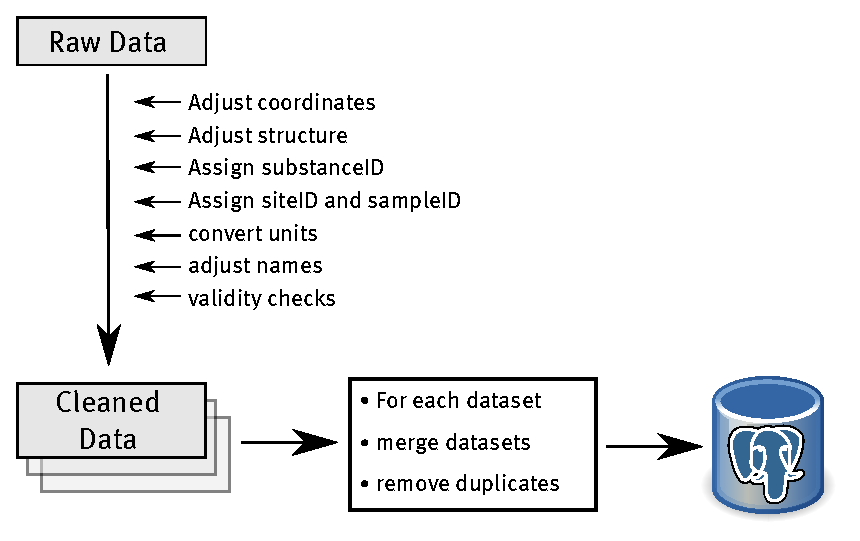
\includegraphics[width = \textwidth]{appendix/smallstreams/one/data_cleaning}
	\caption[Overview on data cleaning steps.]{Overview on data cleaning steps. After cleaning, data have been stored in a relational spatial PostgreSQL database.}
	\label{fig:data_cleaning}
\end{figure}



%% -------------------------------------------------------------------------
\FloatBarrier

\clearpage
\section{Overview on compiled data}
% Overview samples
% table generated in do_overview.R
\begin{sidewaystable}[H]
\centering
\caption[Overview on chemical samples.]{Overview on chemical samples. Only data from running waters and grab
sampling is shown. \textsuperscript{a}: Abbreviations according to ISO 3166-2:DE. 
      \textsuperscript{b}: Including metabolites}\label{tab:phch_overview}
\begin{tabular}{p{2.7cm}lllR{2cm}R{2cm}R{2cm}}
  \toprule
name & abbrv.\textsuperscript{a} & Begin & End & No. sites & No.samples & No. pesticides\textsuperscript{b} \\ 
  \midrule
Baden-Württemberg & BW & 2005-03-10 & 2014-10-02 & 7 & 172 & 98 \\ 
  Bavaria & BY & 2006-04-19 & 2013-12-17 & 13 & 218 & 155 \\ 
  Hesse & HE & 2007-01-15 & 2014-12-18 & 65 & 2411 & 144 \\ 
  Mecklenburg-Western Pomerania & MV & 2005-03-08 & 2014-12-17 & 130 & 1503 & 227 \\ 
  Lower Saxony & NI & 2014-03-24 & 2014-10-13 & 1 & 7 & 226 \\ 
  North Rhine-Westphalia & NW & 2005-01-18 & 2015-01-22 & 1139 & 8536 & 198 \\ 
  Rhineland-Palatinate & RP & 2008-01-02 & 2013-12-18 & 7 & 341 & 236 \\ 
  Schleswig-Holstein & SH & 2005-04-26 & 2014-11-26 & 269 & 1380 & 180 \\ 
  Saarland & SL & 2005-01-03 & 2013-11-25 & 2 & 104 & 57 \\ 
  Saxony & SN & 2005-01-02 & 2013-12-18 & 606 & 9141 & 173 \\ 
  Saxony-Anhalt & ST & 2005-01-24 & 2015-03-19 & 30 & 416 & 88 \\ 
  Thuringia & TH & 2005-06-16 & 2014-12-08 & 32 & 514 & 63 \\ 
   \midrule
 & Total & 2005-01-02 & 2015-03-19 & 2301 & 24743 & 478 \\ 
   \bottomrule
\end{tabular}
\end{sidewaystable}



\clearpage


\begin{landscape}
\begin{figure}[h]
	\centering
	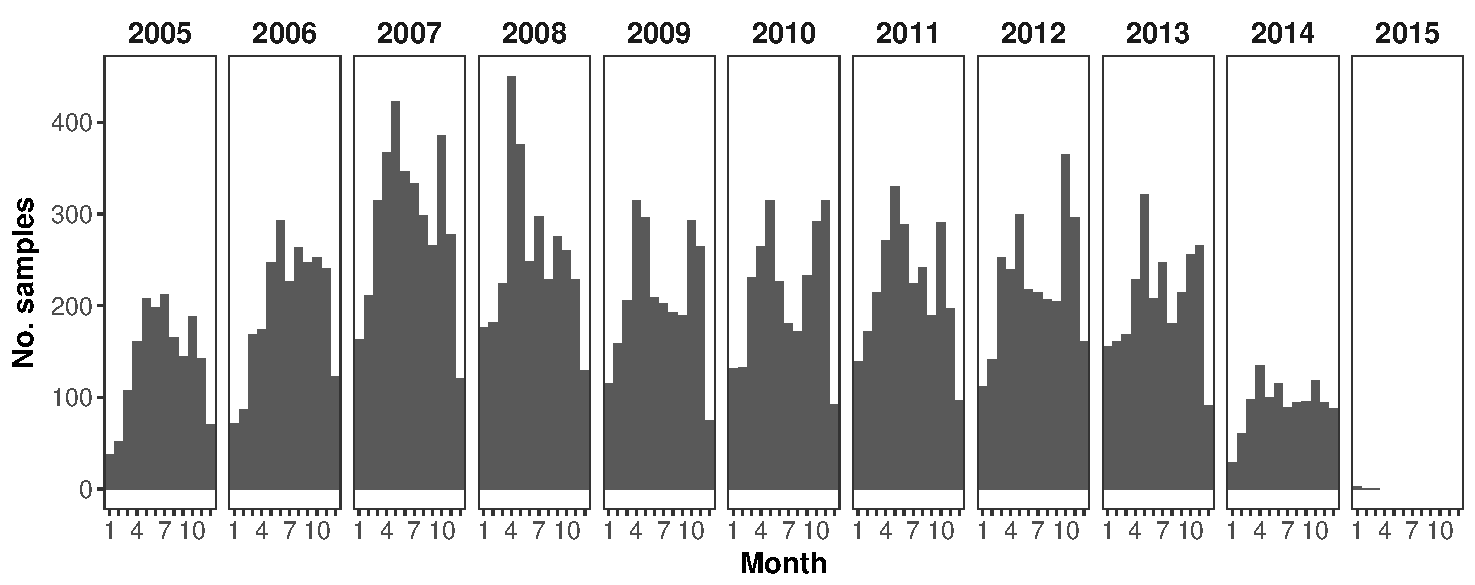
\includegraphics[width = \textheight]{appendix/smallstreams/one/temporal}
	\caption{Number of sampling occasions per year and month.}
	\label{fig:temporal}
\end{figure}
\end{landscape}

\clearpage


\begin{figure}[h]
	\centering
	\vspace{-1.5cm}
	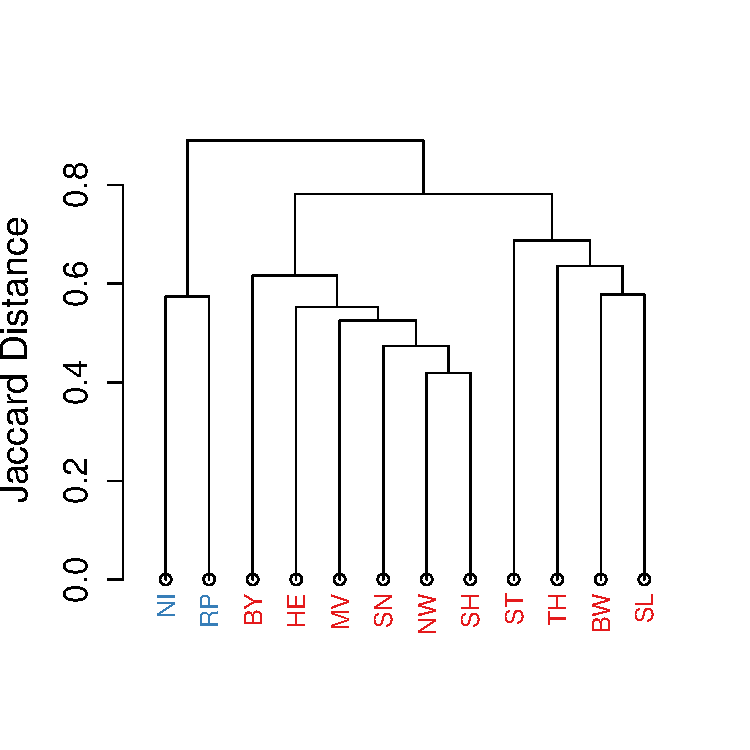
\includegraphics[width = 0.6\textwidth]{appendix/smallstreams/one/varclus}
	\vspace{-1cm}
	\caption[Complete Linkage Cluster Dendrogram of Jaccard Similarity of analysed compound spectra between federal states.]{Complete Linkage Cluster Dendrogram of Jaccard Similarity of analysed compound spectra between federal states. Abbreviations of state names according to ISO 3166-2:DE.}
	\label{fig:varclus}
\end{figure}



\begin{figure}[h]
	\centering
	\vspace{-1.5cm} 
	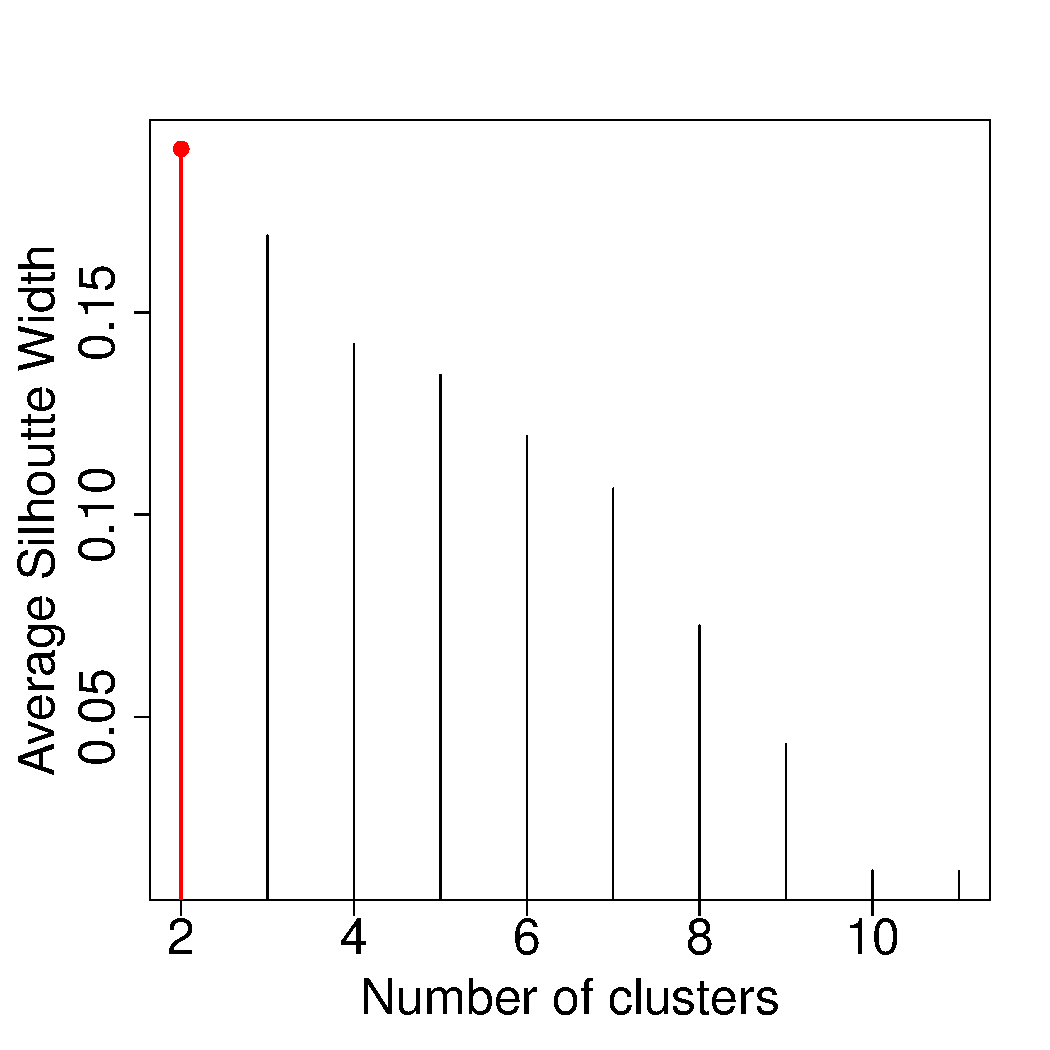
\includegraphics[width = 0.5\textwidth]{appendix/smallstreams/one/silhouette}
	\caption[Average silhouette width for different cluster sizes.]{Average silhouette width for different cluster sizes of complete linkage clustering of jaccard similarity of analysed compound spectra between federal states. Two clusters showed the maximum silhouette width.}
	\label{fig:silhouette}
\end{figure}

% Overview variables
% table generated in do_overview.R
\clearpage
\footnotesize
% -*- root: ../../../thesis.tex -*-

\begin{longtable}{lp{3cm}rlp{1cm}p{1cm}p{1.5cm}}
\caption[Overview on pesticides in the database.]{Overview on pesticides (and metabolites) in the database. \
                    \textsuperscript{a} Authorized in Germany (Source: German Federal Office of Consumer Protection and Food Safety (BVL) as at March 2015). 
                    \textsuperscript{b} Authorized in the European union (Source: EU Pesticides database as at March 2015).
                    \textsuperscript{c} Regulatory Acceptable Concentration [$\mu g/L$] (Source: German Environment Agency (UBA) as at November 2015).} \\ 
  \toprule
 & Name & CAS & Group & Auth. GER\textsuperscript{a} & Auth. EU\textsuperscript{b} & RAC \textsuperscript{c} \\ 
  \midrule
  \endfirsthead
  %
\caption*{\raggedright Table \thetable\ Continued. }\\
        \toprule
 & Name & CAS & Group & Auth. GER\textsuperscript{a} & Auth. EU\textsuperscript{b} & RAC \textsuperscript{c} \\ 
\midrule
\endhead
%
1 & (E)7-(Z)9-Dodecadienylacetat & 55774-32-8 & other & x & x &  \\ 
  2 & (Z)-9-Dodecenylacetat & 16974-11-1 & other & x & x &  \\ 
  3 & 1,3-cis-Dichlorpropen & 10061-01-5 & other &  &  &  \\ 
  4 & 1,3-trans-Dichlorpropen & 10061-02-6 & other &  &  &  \\ 
  5 & 1-(3,4-Dichlorphenyl)urea & 2327-02-8 & metabolite &  &  &  \\ 
  6 & 1-(4-Isopropylphenyl)urea & 56046-17-4 & metabolite &  &  &  \\ 
  7 & 1-Decanol & 112-30-1 & other & x & x &  \\ 
  8 & 1-Methylcyclopropen & 3100-04-7 & other & x & x &  \\ 
  9 & 2,4,5-T & 93-76-5 & herbicide &  &  &  \\ 
  10 & 2,4,6-Trichlorphenol & 88-06-2 & metabolite &  &  &  \\ 
  11 & 2,4-D & 94-75-7 & herbicide & x & x & 1.10000 \\ 
  12 & 2,4-DB & 94-82-6 & herbicide &  & x &  \\ 
  13 & 2,4-Dichlorphenol & 120-83-2 & metabolite &  &  &  \\ 
  14 & 2,6-Dichlorobenzamid & 2008-58-4 & metabolite &  &  &  \\ 
  15 & 2-Hydroxydesethylatrazin & 19988-24-0 & metabolite &  &  &  \\ 
  16 & 3-Hydroxy Carbofuran & 16655-82-6 & metabolite &  &  &  \\ 
  17 & 4,6-Dinitro-o-Cresol & 534-52-1 & insecticide &  &  &  \\ 
  18 & 4-tert. Cyclobutylhexanon & 98-53-3 & metabolite &  &  &  \\ 
  19 & AMPA & 1066-51-9 & metabolite &  &  &  \\ 
  20 & Acequinocyl & 57960-19-7 & insecticide & x & x & 9.00000 \\ 
  21 & Acetamiprid & 135410-20-7 & insecticide & x & x & 0.24000 \\ 
  22 & Acetochlor & 34256-82-1 & herbicide &  &  &  \\ 
  23 & Acetochlorsulfonsäure & 187022-11-3 & metabolite &  &  &  \\ 
  24 & Acetochlorsäure & 194992-44-4 & metabolite &  &  &  \\ 
  25 & Acifluorfen & 50594-66-6 & herbicide &  &  &  \\ 
  26 & Aclonifen & 74070-46-5 & herbicide & x & x & 1.06000 \\ 
  27 & Acrinathrin & 101007-06-1 & insecticide &  & x &  \\ 
  28 & Alachlor & 15972-60-8 & herbicide &  &  &  \\ 
  29 & Aldicarb & 116-06-3 & insecticide &  &  &  \\ 
  30 & Aldrin & 309-00-2 & insecticide &  &  &  \\ 
  31 & Ametoctradin & 865318-97-4 & fungicide & x & x &  \\ 
  32 & Ametryn & 834-12-8 & herbicide &  &  &  \\ 
  33 & Amidosulfuron & 120923-37-7 & herbicide & x & x &  \\ 
  34 & Aminopyralid & 150114-71-9 & herbicide & x & x &  \\ 
  35 & Amisulbrom & 348635-87-0 & fungicide & x & x &  \\ 
  36 & Anthranilsäure\-isopropylamid & 30391-89-0 & metabolite &  &  &  \\ 
  37 & Atraton & 1610-17-9 & herbicide &  &  &  \\ 
  38 & Atrazin & 1912-24-9 & herbicide &  &  &  \\ 
  39 & Atrazin, 2-Hydroxy & 2163-68-0 & metabolite &  &  &  \\ 
  40 & Avermectin B1a & 71751-41-2 & insecticide & x & x &  \\ 
  41 & Azadirachtin (Neem) & 11141-17-6 & insecticide & x & x &  \\ 
  42 & Azinphos-ethyl & 2642-71-9 & insecticide &  &  &  \\ 
  43 & Azinphos-methyl & 86-50-0 & insecticide &  &  &  \\ 
  44 & Aziprotryn & 4658-28-0 & herbicide &  &  &  \\ 
  45 & Azoxystrobin & 131860-33-8 & fungicide & x & x & 0.55000 \\ 
  46 & Azoxystrobin-CA &  & metabolite &  &  &  \\ 
  47 & Beflubutamid & 113614-08-7 & herbicide & x & x &  \\ 
  48 & Benalaxyl & 71626-11-4 & fungicide & x & x & 20.00000 \\ 
  49 & Benazolin & 3813-05-6 & herbicide &  &  &  \\ 
  50 & Bensulfuron-methyl & 83055-99-6 & herbicide &  & x &  \\ 
  51 & Bentazon & 25057-89-0 & herbicide & x & x & 535.00000 \\ 
  52 & Benthiavalicarb & 413615-35-7 & fungicide & x & x &  \\ 
  53 & Benzoesäure & 65-85-0 & fungicide & x & x &  \\ 
  54 & Betacypermethrin & 65731-84-2 & insecticide &  & x &  \\ 
  55 & Bifenazate & 149877-41-8 & insecticide & x & x &  \\ 
  56 & Bifenox & 42576-02-3 & herbicide & x & x &  \\ 
  57 & Bifenthrin & 82657-04-3 & insecticide &  & x & 0.00050 \\ 
  58 & Bixafen & 581809-46-3 & fungicide & x & x & 0.46000 \\ 
  59 & Boscalid & 188425-85-6 & fungicide & x & x & 12.50000 \\ 
  60 & Bromacil & 314-40-9 & herbicide &  &  &  \\ 
  61 & Bromadiolon & 28772-56-7 & other &  & x &  \\ 
  62 & Bromocyclen & 1715-40-8 & insecticide &  &  &  \\ 
  63 & Bromoxynil & 1689-84-5 & herbicide & x & x & 3.30000 \\ 
  64 & Bupirimat & 41483-43-6 & fungicide &  & x &  \\ 
  65 & Buturon & 3766-60-7 & herbicide &  &  &  \\ 
  66 & Captan & 133-06-2 & fungicide & x & x & 5.00000 \\ 
  67 & Carbendazim & 10605-21-7 & fungicide &  &  & 0.15000 \\ 
  68 & Carbetamid & 16118-49-3 & herbicide &  & x &  \\ 
  69 & Carbofuran & 1563-66-2 & insecticide &  &  &  \\ 
  70 & Carboxin & 5234-68-4 & fungicide &  & x &  \\ 
  71 & Carfentrazone-ethyl & 128639-02-1 & herbicide & x & x & 0.31000 \\ 
  72 & Chloramben & 133-90-4 & herbicide &  &  &  \\ 
  73 & Chlorantraniliprole & 500008-45-7 & insecticide & x & x & 0.35500 \\ 
  74 & Chlorbromuron & 13360-45-7 & herbicide &  &  &  \\ 
  75 & Chlordan & 57-74-9 & insecticide &  &  &  \\ 
  76 & Chlorfenac & 85-34-7 & herbicide &  &  &  \\ 
  77 & Chlorfenvinphos & 470-90-6 & insecticide &  &  &  \\ 
  78 & Chlorfluazuron & 71422-67-8 & insecticide &  &  &  \\ 
  79 & Chloridazon & 1698-60-8 & herbicide & x & x & 56.00000 \\ 
  80 & Chlormequat & 7003-89-6 & other & x & x &  \\ 
  81 & Chloroxuron & 1982-47-4 & herbicide &  &  &  \\ 
  82 & Chlorpropham & 101-21-3 & herbicide & x & x &  \\ 
  83 & Chlorpyrifos & 2921-88-2 & insecticide &  & x & 0.00050 \\ 
  84 & Chlorpyriphos methyl & 5598-13-0 & insecticide &  & x &  \\ 
  85 & Chlorsulfuron & 64902-72-3 & herbicide &  &  &  \\ 
  86 & Chlorthalonil & 1897-45-6 & fungicide & x & x &  \\ 
  87 & Chlorthalonil-SA &  & metabolite &  &  &  \\ 
  88 & Chlortoluron & 15545-48-9 & herbicide & x & x & 2.30000 \\ 
  89 & Cinidon-ethyl & 142891-20-1 & herbicide &  &  &  \\ 
  90 & Clethodim & 99129-21-2 & herbicide & x & x &  \\ 
  91 & Clodinafop & 114420-56-3 & herbicide & x & x &  \\ 
  92 & Clodinafop-propargyl & 105512-06-9 & herbicide &  &  &  \\ 
  93 & Clofentezin & 74115-24-5 & insecticide &  & x &  \\ 
  94 & Clomazon & 81777-89-1 & herbicide & x & x & 5.70000 \\ 
  95 & Clopyralid & 1702-17-6 & herbicide & x & x & 1080.00000 \\ 
  96 & Cloquintocet-mexyl & 99607-70-2 & other &  & x &  \\ 
  97 & Clothianidin & 210880-92-5 & insecticide & x & x & 0.00700 \\ 
  98 & Codlemone (Codlelure) & 33956-49-9 & other & x & x &  \\ 
  99 & Coumaphos & 56-72-4 & insecticide &  &  &  \\ 
  100 & Crimidin & 535-89-7 & other &  &  &  \\ 
  101 & Cyanazin & 21725-46-2 & herbicide &  &  &  \\ 
  102 & Cyazofamid & 120116-88-3 & fungicide & x & x &  \\ 
  103 & Cyclanilide & 113136-77-9 & other &  &  &  \\ 
  104 & Cycloat & 1134-23-2 & herbicide &  &  &  \\ 
  105 & Cycloxidim & 101205-02-1 & herbicide & x & x &  \\ 
  106 & Cyflufenamid & 180409-60-3 & fungicide & x & x &  \\ 
  107 & Cyfluthrin (Summe Isomere) & 68359-37-5 & insecticide &  &  &  \\ 
  108 & Cyhalothrin (Summe Isomere) & 91465-08-6 & insecticide & x & x &  \\ 
  109 & Cymoxanil & 57966-95-7 & fungicide & x & x & 4.40000 \\ 
  110 & Cypermetryn & 52315-07-8 & insecticide & x & x & 0.00100 \\ 
  111 & Cyproconazol & 94361-06-5 & fungicide & x & x &  \\ 
  112 & Cyprodinil & 121552-61-2 & fungicide & x & x & 0.75000 \\ 
  113 & Cyromazin & 66215-27-8 & insecticide &  & x &  \\ 
  114 & Daminozid & 1596-84-5 & other & x & x &  \\ 
  115 & Deiquat & 2764-72-9 & herbicide & x & x &  \\ 
  116 & Deltamethrin & 52918-63-5 & insecticide & x & x &  \\ 
  117 & Demeton-O & 298-03-3 & insecticide &  &  &  \\ 
  118 & Demeton-S & 126-75-0 & insecticide &  &  &  \\ 
  119 & Demeton-S-methyl & 919-86-8 & insecticide &  &  &  \\ 
  120 & Demeton-S-methylsulfon & 17040-19-6 & insecticide &  &  &  \\ 
  121 & Desaminometribuzin & 35045-02-4 & metabolite &  &  &  \\ 
  122 & Desethyl-2-hydroxyterbuthylazin & 66753-06-8 & metabolite &  &  &  \\ 
  123 & Desethylatrazin & 6190-65-4 & metabolite &  &  &  \\ 
  124 & Desethylsebuthylazin & 37019-18-4 & metabolite &  &  &  \\ 
  125 & Desethylsimazin & 6190-65-4 & metabolite &  &  &  \\ 
  126 & Desethylterbuthylazin & 30125-63-4 & metabolite &  &  &  \\ 
  127 & Desisopropylatrazin & 1007-28-9 & metabolite &  &  &  \\ 
  128 & Desmedipham & 13684-56-5 & herbicide & x & x &  \\ 
  129 & Desmethyldiuron & 3567-62-2 & metabolite &  &  &  \\ 
  130 & Desmethylisoproturon & 34123-57-4 & metabolite &  &  &  \\ 
  131 & Desmetryn & 1014-69-3 & herbicide &  &  &  \\ 
  132 & Desphenyl-Chloridazon & 6339-19-1 & metabolite &  &  &  \\ 
  133 & Diazinon & 333-41-5 & insecticide &  &  &  \\ 
  134 & Dicamba & 1918-00-9 & herbicide & x & x & 180.00000 \\ 
  135 & Dichlobenil & 1194-65-6 & herbicide &  &  &  \\ 
  136 & Dichlofluanid & 1085-98-9 & fungicide &  &  &  \\ 
  137 & Dichlorprop & 120-36-5 & herbicide &  &  &  \\ 
  138 & Dichlorprop-P & 15165-67-0 & herbicide & x & x &  \\ 
  139 & Dichlorvos & 62-73-7 & insecticide &  &  &  \\ 
  140 & Diclofop & 40843-25-2 & herbicide &  & x &  \\ 
  141 & Dicofol & 115-32-2 & insecticide &  &  &  \\ 
  142 & Dieldrin & 60-57-1 & insecticide &  &  &  \\ 
  143 & Difenacoum & 56073-07-5 & other &  & x &  \\ 
  144 & Difenoconazol & 119446-68-3 & fungicide & x & x & 0.36000 \\ 
  145 & Diflubenzuron & 35367-38-5 & insecticide &  & x &  \\ 
  146 & Diflufenican & 83164-33-4 & herbicide & x & x & 0.02500 \\ 
  147 & Dimefuron & 34205-21-5 & herbicide &  &  & 0.83000 \\ 
  148 & Dimethachlor & 50563-36-5 & herbicide & x & x & 3.50000 \\ 
  149 & Dimethachlor-CA &  & metabolite &  &  &  \\ 
  150 & Dimethachlor\-sulfonsäure &  & metabolite &  &  &  \\ 
  151 & Dimethachlorsäure &  & metabolite &  &  &  \\ 
  152 & Dimethenamid & 87674-68-8 & herbicide &  &  &  \\ 
  153 & Dimethenamid-CA &  & metabolite &  &  &  \\ 
  154 & Dimethenamid-P & 163515-14-8 & herbicide & x & x & 1.35000 \\ 
  155 & Dimethenamid-SA &  & metabolite &  &  &  \\ 
  156 & Dimethenamid\-sulfonsäure &  & metabolite &  &  &  \\ 
  157 & Dimethoat & 60-51-5 & insecticide & x & x & 4.00000 \\ 
  158 & Dimethomorph & 110488-70-5 & fungicide & x & x & 5.60000 \\ 
  159 & Dimoxystrobin & 149961-52-4 & fungicide & x & x & 0.03160 \\ 
  160 & Diniconazol & 83657-24-3 & fungicide &  &  &  \\ 
  161 & Dinoseb & 88-85-7 & herbicide &  &  &  \\ 
  162 & Dinotefuran & 165252-70-0 & insecticide &  &  &  \\ 
  163 & Dinoterb & 1420-07-1 & herbicide &  &  &  \\ 
  164 & Disulfoton & 298-04-4 & insecticide &  &  &  \\ 
  165 & Dithianon & 3347-22-6 & fungicide & x & x & 0.78000 \\ 
  166 & Diuron & 330-54-1 & herbicide &  & x & 0.79000 \\ 
  167 & Dodin & 2439-10-3 & fungicide & x & x & 5.33000 \\ 
  168 & Endosulfan, alpha & 959-98-8 & insecticide &  &  &  \\ 
  169 & Endosulfan, beta & 33213-65-9 & insecticide &  &  &  \\ 
  170 & Endosulfansulfat & 1031-07-8 & metabolite &  &  &  \\ 
  171 & Endrin & 72-20-8 & insecticide &  &  &  \\ 
  172 & Epoxiconazol & 133855-98-8 & fungicide & x & x & 0.53750 \\ 
  173 & Esfenvalerat & 66230-04-4 & insecticide & x & x &  \\ 
  174 & Etaconazol & 60207-93-4 & fungicide &  &  &  \\ 
  175 & Ethidimuron & 30043-49-3 & herbicide &  &  &  \\ 
  176 & Ethirimol & 23947-60-6 & fungicide &  &  &  \\ 
  177 & Ethofenprox & 80844-07-1 & insecticide & x & x &  \\ 
  178 & Ethofumesat & 26225-79-6 & herbicide & x & x & 24.00000 \\ 
  179 & Etrimfos & 38260-54-7 & insecticide &  &  &  \\ 
  180 & Famoxadone & 131807-57-3 & fungicide & x & x &  \\ 
  181 & Fenamidon & 161326-34-7 & fungicide & x & x &  \\ 
  182 & Fenamiphos & 22224-92-6 & insecticide &  & x &  \\ 
  183 & Fenarimol & 60168-88-9 & fungicide &  &  &  \\ 
  184 & Fenazaquin & 120928-09-8 & insecticide & x & x &  \\ 
  185 & Fenhexamid & 126833-17-8 & fungicide & x & x & 10.10000 \\ 
  186 & Fenitrothion & 122-14-5 & insecticide &  &  &  \\ 
  187 & Fenoprop & 93-72-1 & herbicide &  &  &  \\ 
  188 & Fenoxaprop & 95617-09-7 & herbicide &  &  &  \\ 
  189 & Fenoxaprop-p & 113158-40-0 & herbicide & x & x &  \\ 
  190 & Fenoxaprop-p-ethyl & 71283-80-2 & herbicide &  &  &  \\ 
  191 & Fenoxycarb & 72490-01-8 & insecticide &  & x &  \\ 
  192 & Fenpropidin & 67306-00-7 & fungicide & x & x &  \\ 
  193 & Fenpropimorph & 67564-91-4 & fungicide & x & x & 0.19500 \\ 
  194 & Fenpyroximat & 134098-61-6 & insecticide & x & x &  \\ 
  195 & Fenthion & 55-38-9 & insecticide &  &  &  \\ 
  196 & Fenuron & 101-42-8 & herbicide &  &  &  \\ 
  197 & Fipronil & 120068-37-3 & insecticide &  & x & 0.00077 \\ 
  198 & Flamprop & 58667-63-3 & herbicide &  &  &  \\ 
  199 & Flazasulfuron & 104040-78-0 & herbicide & x & x &  \\ 
  200 & Flonicamid & 158062-67-0 & insecticide & x & x & 310.00000 \\ 
  201 & Florasulam & 145701-23-1 & herbicide & x & x &  \\ 
  202 & Fluazifop & 69335-91-7 & herbicide &  &  & 146.00000 \\ 
  203 & Fluazifop-P & 83066-88-0 & herbicide & x & x & 146.00000 \\ 
  204 & Fluazifop-P-butyl & 79241-46-6 & herbicide &  &  & 7.70000 \\ 
  205 & Fluazifop-butyl & 69806-50-4 & herbicide &  &  & 7.70000 \\ 
  206 & Fluazinam & 79622-59-6 & fungicide & x & x & 0.26000 \\ 
  207 & Fluchloralin & 33245-39-5 & herbicide &  &  &  \\ 
  208 & Fludioxonil & 131341-86-1 & fungicide & x & x & 0.50000 \\ 
  209 & Flufenacet & 142459-58-3 & herbicide & x & x & 2.40000 \\ 
  210 & Flufenacet-SA &  & metabolite &  &  &  \\ 
  211 & Flufenoxuron & 101463-69-8 & insecticide &  &  &  \\ 
  212 & Flumioxazin & 103361-09-7 & herbicide & x & x &  \\ 
  213 & Fluometuron & 2164-17-2 & herbicide &  & x &  \\ 
  214 & Fluopicolide & 239110-15-7 & fungicide & x & x &  \\ 
  215 & Fluopyram & 658066-35-4 & fungicide & x & x & 5.12000 \\ 
  216 & Fluoxastrobin & 361377-29-9 & fungicide & x & x &  \\ 
  217 & Flupyrsulfuron & 150315-10-9 & herbicide & x & x &  \\ 
  218 & Fluquinconazole & 136426-54-5 & fungicide & x & x & 0.80000 \\ 
  219 & Flurochloridon & 61213-25-0 & herbicide &  & x &  \\ 
  220 & Fluroxypyr & 69377-81-7 & herbicide & x & x & 16.00000 \\ 
  221 & Fluroxypyr-methylheptyl & 81406-37-3 & herbicide &  &  &  \\ 
  222 & Flurtamone & 96525-23-4 & herbicide & x & x & 0.99000 \\ 
  223 & Flusilazol & 85509-19-9 & fungicide &  &  & 1.10000 \\ 
  224 & Flutolanil & 66332-96-5 & fungicide & x & x &  \\ 
  225 & Flutriafol & 76674-21-0 & fungicide &  & x &  \\ 
  226 & Fluxapyroxad & 907204-31-3 & fungicide & x & x &  \\ 
  227 & Folpet & 133-07-3 & fungicide & x & x &  \\ 
  228 & Foramsulfuron & 173159-57-4 & herbicide & x & x & 0.09500 \\ 
  229 & Fosetyl & 15845-66-6 & fungicide & x & x &  \\ 
  230 & Fosthiazat & 98886-44-3 & other & x & x &  \\ 
  231 & Fuberidazol & 3878-19-1 & fungicide & x & x &  \\ 
  232 & Furalaxyl & 57646-30-7 & fungicide &  &  &  \\ 
  233 & Furmecyclox & 60568-05-0 & fungicide &  &  &  \\ 
  234 & Glufosinat & 51276-47-2 & herbicide & x & x &  \\ 
  235 & Glyphosate & 1071-83-6 & herbicide & x & x & 100.00000 \\ 
  236 & HCH, gamma (Lindan) & 58-89-9 & insecticide &  &  &  \\ 
  237 & Haloxyfop & 69806-34-4 & herbicide &  &  &  \\ 
  238 & Haloxyfop-P & 95977-29-0 & herbicide & x & x &  \\ 
  239 & Haloxyfop-ethoxyethyl & 87237-48-7 & herbicide &  &  &  \\ 
  240 & Heptachlor & 76-44-8 & insecticide &  &  &  \\ 
  241 & Heptachlorepoxid & 1024-57-3 & metabolite &  &  &  \\ 
  242 & Heptenophos & 23560-59-0 & insecticide &  &  &  \\ 
  243 & Hexachlorbenzen & 118-74-1 & fungicide &  &  &  \\ 
  244 & Hexachlorophen & 70-30-4 & other &  &  &  \\ 
  245 & Hexaconazol & 79983-71-4 & fungicide &  &  &  \\ 
  246 & Hexaflumuron & 86479-06-3 & insecticide &  &  &  \\ 
  247 & Hexazinon & 51235-04-2 & herbicide &  &  &  \\ 
  248 & Hexythiazox & 78587-05-0 & insecticide & x & x &  \\ 
  249 & Hymexazol & 10004-44-1 & fungicide & x & x &  \\ 
  250 & Icaridinsäure &  & metabolite &  &  &  \\ 
  251 & Imazalil & 35554-44-0 & fungicide & x & x &  \\ 
  252 & Imazamox & 114311-32-9 & herbicide & x & x &  \\ 
  253 & Imazapic & 104098-48-8 & herbicide &  &  &  \\ 
  254 & Imazaquin & 81335-37-7 & herbicide &  & x &  \\ 
  255 & Imazethapyr & 81335-77-5 & herbicide &  &  &  \\ 
  256 & Imazosulfuron & 122548-33-8 & herbicide & x & x &  \\ 
  257 & Imidacloprid & 138261-41-3 & insecticide & x & x & 0.00900 \\ 
  258 & Indoxacarb & 173584-44-6 & insecticide & x & x &  \\ 
  259 & Iodosulfuron & 185119-76-0 & herbicide & x & x & 0.07900 \\ 
  260 & Iodosulfuron-methyl & 144550-06-1 & herbicide &  &  &  \\ 
  261 & Iodosulfuron-methyl-sodium & 144550-36-7 & herbicide &  &  &  \\ 
  262 & Ioxynil & 1689-83-4 & herbicide & x &  & 2.70000 \\ 
  263 & Iprodion & 36734-19-7 & fungicide & x & x &  \\ 
  264 & Iprovalicarb & 140923-17-7 & fungicide & x & x & 189.00000 \\ 
  265 & Isodrin & 465-73-6 & insecticide &  &  &  \\ 
  266 & Isophenphos & 25311-71-1 & insecticide &  &  &  \\ 
  267 & Isoproturon & 34123-59-6 & herbicide & x & x & 1.30000 \\ 
  268 & Isopyrazam & 881685-58-1 & fungicide & x & x &  \\ 
  269 & Isoxaben & 82558-50-7 & herbicide & x & x &  \\ 
  270 & Isoxaflutole & 141112-29-0 & herbicide & x & x &  \\ 
  271 & Karbutylat & 4849-32-5 & herbicide &  &  &  \\ 
  272 & Kresoxim-methyl & 143390-89-0 & fungicide & x & x & 1.00000 \\ 
  273 & Kresoximsäure &  & metabolite &  &  &  \\ 
  274 & Lenacil & 2164-08-1 & herbicide & x & x & 0.65000 \\ 
  275 & Linuron & 330-55-2 & herbicide &  & x &  \\ 
  276 & MCPA & 94-74-6 & herbicide & x & x & 9.00000 \\ 
  277 & MCPB & 94-81-5 & herbicide &  & x &  \\ 
  278 & Malathion & 121-75-5 & insecticide &  & x &  \\ 
  279 & Mancozeb & 8018-01-7 & fungicide & x & x & 0.21900 \\ 
  280 & Mandipropamid & 374726-62-2 & fungicide & x & x & 7.60000 \\ 
  281 & Maneb & 12427-38-2 & fungicide & x & x &  \\ 
  282 & Mecoprop & 93-65-2 & herbicide &  & x & 160.00000 \\ 
  283 & Mefenpyr-diethyl & 135591-00-3 & other & x &  &  \\ 
  284 & Mepanipyrim & 110235-47-7 & fungicide & x & x &  \\ 
  285 & Mepiquat & 15302-91-7 & other & x & x &  \\ 
  286 & Mepronil & 55814-41-0 & fungicide &  &  &  \\ 
  287 & Meptyldinocap & 131-72-6 & fungicide &  & x &  \\ 
  288 & Mesosulfuron & 400852-66-6 & herbicide & x & x &  \\ 
  289 & Mesotrion & 104206-82-8 & herbicide & x & x &  \\ 
  290 & Metaflumizone & 139968-49-3 & insecticide & x & x &  \\ 
  291 & Metalaxyl & 57837-19-1 & fungicide &  & x & 46.00000 \\ 
  292 & Metalaxyl-CA & 75596-99-5 & metabolite &  &  &  \\ 
  293 & Metalaxyl-CA2 & 104390-56-9 & metabolite &  &  &  \\ 
  294 & Metalaxyl-M & 70630-17-0 & fungicide & x & x & 46.00000 \\ 
  295 & Metaldehyd & 108-62-3 & other & x & x &  \\ 
  296 & Metamitron & 41394-05-2 & herbicide & x & x & 38.00000 \\ 
  297 & Metamitron-Desamino & 36993-94-9 & metabolite &  &  &  \\ 
  298 & Metazachlor & 67129-08-2 & herbicide & x & x & 0.88000 \\ 
  299 & Metazachlor\-dicarbonsäure &  & metabolite &  &  &  \\ 
  300 & Metazachlor\-sulfonsäure & 172960-62-2 & metabolite &  &  &  \\ 
  301 & Metazachlorsäure & 1231244-60-2 & metabolite &  &  &  \\ 
  302 & Metconazol & 125116-23-6 & fungicide & x & x &  \\ 
  303 & Methabenzthiazuron & 18691-97-9 & herbicide &  &  &  \\ 
  304 & Methamidophos & 10265-92-6 & insecticide &  &  & 2.60000 \\ 
  305 & Methidathion & 950-37-8 & insecticide &  &  &  \\ 
  306 & Methiocarb & 2032-65-7 & insecticide & x & x & 0.01000 \\ 
  307 & Methobromuron & 3060-89-7 & herbicide &  & x & 2.00000 \\ 
  308 & Methomyl & 16752-77-5 & insecticide &  & x &  \\ 
  309 & Methoprotryn & 841-06-5 & herbicide &  &  &  \\ 
  310 & Methoxychlor & 72-43-5 & insecticide &  &  &  \\ 
  311 & Methoxyfenozid & 161050-58-4 & insecticide & x & x &  \\ 
  312 & Methyldesphenyl-Chloridazon & 17254-80-7 & metabolite &  &  &  \\ 
  313 & Metiram & 9006-42-2 & fungicide & x & x &  \\ 
  314 & Metolachlor & 51218-45-2 & herbicide &  &  &  \\ 
  315 & Metolachlor\-sulfonsäure & 171118-09-5 & metabolite &  &  &  \\ 
  316 & Metolachlorsäure & 152019-73-3 & metabolite &  &  &  \\ 
  317 & Metosulam & 139528-85-1 & herbicide & x & x &  \\ 
  318 & Metoxuron & 19937-59-8 & herbicide &  &  &  \\ 
  319 & Metrafenon & 220899-03-6 & fungicide & x & x &  \\ 
  320 & Metribuzin & 21087-64-9 & herbicide & x & x & 0.58400 \\ 
  321 & Metsulfuron & 79510-48-8 & herbicide & x & x &  \\ 
  322 & Metsulfuron-methyl & 74223-64-6 & herbicide &  &  &  \\ 
  323 & Mevinphos & 7786-34-7 & insecticide &  &  &  \\ 
  324 & Milbemectin & 51596-11-3 & insecticide & x & x &  \\ 
  325 & Mirex & 2385-85-5 & insecticide &  &  &  \\ 
  326 & Monolinuron & 1746-81-2 & herbicide &  &  &  \\ 
  327 & Monuron & 150-68-5 & herbicide &  &  &  \\ 
  328 & Myclobutanil & 88671-89-0 & fungicide & x & x & 2.40000 \\ 
  329 & Napropamid & 15299-99-7 & herbicide & x & x & 6.70000 \\ 
  330 & Neburon & 555-37-3 & herbicide &  &  &  \\ 
  331 & Nicosulfuron & 111991-09-4 & herbicide & x & x & 0.08500 \\ 
  332 & Nitenpyram & 120738-89-8 & insecticide &  &  &  \\ 
  333 & Nitrofen & 1836-75-5 & herbicide &  &  &  \\ 
  334 & Norflurazon & 27314-13-2 & herbicide &  &  &  \\ 
  335 & Omethoat & 1113-02-6 & insecticide &  &  &  \\ 
  336 & Orysastrobin & 248593-16-0 & fungicide &  &  &  \\ 
  337 & Oxadiazon & 19666-30-9 & herbicide &  & x &  \\ 
  338 & Oxadixyl & 77732-09-3 & fungicide &  &  &  \\ 
  339 & Oxamyl & 23135-22-0 & insecticide &  & x &  \\ 
  340 & Oxydemeton-methyl & 301-12-2 & insecticide &  &  & 1.10000 \\ 
  341 & Paclobutrazol & 76738-62-0 & other & x & x &  \\ 
  342 & Parathion-ethyl & 56-38-2 & insecticide &  &  &  \\ 
  343 & Parathion-methyl & 298-00-0 & insecticide &  &  &  \\ 
  344 & Pelargonsäure & 112-05-0 & herbicide & x & x &  \\ 
  345 & Penconazol & 66246-88-6 & fungicide & x & x & 3.20000 \\ 
  346 & Pencycuron & 66063-05-6 & fungicide & x & x &  \\ 
  347 & Pendimethalin & 40487-42-1 & herbicide & x & x & 0.63000 \\ 
  348 & Penflufen & 494793-67-8 & fungicide &  & x &  \\ 
  349 & Penoxsulam & 219714-96-2 & herbicide & x & x &  \\ 
  350 & Permethrin & 52645-53-1 & insecticide &  &  &  \\ 
  351 & Pethoxamid & 106700-29-2 & herbicide & x & x & 1.77200 \\ 
  352 & Phenmedipham & 13684-63-4 & herbicide & x & x &  \\ 
  353 & Phoxim & 14816-18-3 & insecticide &  &  & 0.00700 \\ 
  354 & Picloram & 1918-02-1 & herbicide & x & x &  \\ 
  355 & Picolinafen & 137641-05-5 & herbicide & x & x & 0.03600 \\ 
  356 & Picoxystrobin & 117428-22-5 & fungicide & x & x & 0.60000 \\ 
  357 & Pinoxaden & 243973-20-8 & herbicide & x &  &  \\ 
  358 & Pirimicarb & 23103-98-2 & insecticide & x & x & 0.09000 \\ 
  359 & Pirimicarb-desmethyl & 30614-22-3 & metabolite &  &  &  \\ 
  360 & Pirimiphos-ethyl & 23505-41-1 & insecticide &  &  &  \\ 
  361 & Pirimiphos-methyl & 29232-93-7 & insecticide & x & x &  \\ 
  362 & Primisulfuron-methyl & 86209-51-0 & herbicide &  &  &  \\ 
  363 & Prochloraz & 67747-09-5 & fungicide & x & x & 5.00000 \\ 
  364 & Procymidon & 32809-16-8 & fungicide &  &  &  \\ 
  365 & Profoxydim & 139001-49-3 & herbicide &  & x &  \\ 
  366 & Prohexadion & 88805-35-0 & other & x & x &  \\ 
  367 & Prometryn & 7287-19-6 & herbicide &  &  &  \\ 
  368 & Propachlor & 1918-16-7 & herbicide &  &  &  \\ 
  369 & Propamocarb & 24579-73-5 & fungicide & x & x &  \\ 
  370 & Propanil & 709-98-8 & herbicide &  &  &  \\ 
  371 & Propaquizafop & 111479-05-1 & herbicide & x & x &  \\ 
  372 & Propazin & 139-40-2 & herbicide &  &  &  \\ 
  373 & Propetamphos & 31218-83-4 & insecticide &  &  &  \\ 
  374 & Propham & 122-42-9 & herbicide &  &  &  \\ 
  375 & Propiconazol & 60207-90-1 & fungicide & x & x & 2.00000 \\ 
  376 & Propoxur & 114-26-1 & insecticide &  &  &  \\ 
  377 & Propoxycarbazone & 145026-81-9 & herbicide & x & x &  \\ 
  378 & Propyzamid & 23950-58-5 & herbicide & x & x & 34.00000 \\ 
  379 & Proquinazid & 189278-12-4 & fungicide & x & x &  \\ 
  380 & Prosulfocarb & 52888-80-9 & herbicide & x & x & 3.80000 \\ 
  381 & Prosulfuron & 94125-34-5 & herbicide & x & x &  \\ 
  382 & Prothioconazol & 178928-70-6 & fungicide & x & x & 1.71000 \\ 
  383 & Prothioconazol-desthio & 120983-64-4 & metabolite &  &  &  \\ 
  384 & Pymetrozin & 123312-89-0 & insecticide & x & x &  \\ 
  385 & Pyraclostrobin & 175013-18-0 & fungicide & x & x &  \\ 
  386 & Pyraflufen & 129630-17-7 & herbicide & x & x &  \\ 
  387 & Pyrazophos & 13457-18-6 & fungicide &  &  &  \\ 
  388 & Pyrethrum & 8003-34-7 & insecticide & x & x & 0.01400 \\ 
  389 & Pyridaben & 96489-71-3 & insecticide &  & x &  \\ 
  390 & Pyridat & 55512-33-9 & herbicide & x & x &  \\ 
  391 & Pyrifenox & 88283-41-4 & fungicide &  &  &  \\ 
  392 & Pyrimethanil & 53112-28-0 & fungicide & x & x & 8.00000 \\ 
  393 & Pyroxsulam & 422556-08-9 & herbicide & x & x &  \\ 
  394 & Quinalphos & 13593-03-8 & insecticide &  &  &  \\ 
  395 & Quinmerac & 90717-03-6 & herbicide & x & x & 316.00000 \\ 
  396 & Quinoclamin & 2797-51-5 & herbicide & x & x &  \\ 
  397 & Quinoxyfen (5,7-di\-chloro-4-(p-fluoro\-phenoxy)\-quinoline) & 124495-18-7 & fungicide & x & x &  \\ 
  398 & Quintozen & 82-68-8 & fungicide &  &  &  \\ 
  399 & Quizalofop & 76578-12-6 & herbicide &  &  &  \\ 
  400 & Quizalofop-ethyl & 76578-14-8 & herbicide &  &  &  \\ 
  401 & Rimsulfuron & 122931-48-0 & herbicide & x & x & 0.46000 \\ 
  402 & Saflufenacil & 372137-35-4 & herbicide &  &  &  \\ 
  403 & Sebuthylazin & 7286-69-3 & herbicide &  &  &  \\ 
  404 & Secbumeton & 26259-45-0 & herbicide &  &  &  \\ 
  405 & Silthiofam & 175217-20-6 & fungicide & x & x &  \\ 
  406 & Simazin & 122-34-9 & herbicide &  &  &  \\ 
  407 & Simazin, 2-Hydroxy & 2599-11-3 & metabolite &  &  &  \\ 
  408 & Spinosad & 168316-95-8 & insecticide & x & x & 0.06200 \\ 
  409 & Spirodiclofen & 148477-71-8 & insecticide & x & x &  \\ 
  410 & Spiromesifen & 283594-90-1 & insecticide &  & x &  \\ 
  411 & Spiroxamin & 118134-30-8 & fungicide & x & x & 0.13000 \\ 
  412 & Sulcotrion & 99105-77-8 & herbicide & x & x &  \\ 
  413 & Sulfosulfuron & 141776-32-1 & herbicide &  & x &  \\ 
  414 & Sulfurylfluorid & 2699-79-8 & insecticide & x & x &  \\ 
  415 & Tebuconazol & 107534-96-3 & fungicide & x & x & 0.57800 \\ 
  416 & Tebufenozid & 112410-23-8 & insecticide & x & x &  \\ 
  417 & Tebufenpyrad & 119168-77-3 & insecticide & x & x &  \\ 
  418 & Tebutam & 35256-85-0 & herbicide &  &  &  \\ 
  419 & Teflubenzuron & 83121-18-0 & insecticide &  & x &  \\ 
  420 & Tefluthrin & 79538-32-2 & insecticide & x & x &  \\ 
  421 & Telodrin & 297-78-9 & insecticide &  &  &  \\ 
  422 & Tembotrione & 335104-84-2 & herbicide & x & x &  \\ 
  423 & Tepraloxydim & 149979-41-9 & herbicide & x & x &  \\ 
  424 & Terbumeton & 33693-04-8 & herbicide &  &  &  \\ 
  425 & Terbuthylazin & 5915-41-3 & herbicide & x & x & 1.20000 \\ 
  426 & Terbutryn & 886-50-0 & herbicide &  &  &  \\ 
  427 & Terbutylazin-Metabolit CGA 324007 & 309923-18-0 & metabolite &  &  &  \\ 
  428 & Terbutylazin-Metabolit SYN 545666 &  & metabolite &  &  &  \\ 
  429 & Tetraconazol & 112281-77-3 & fungicide & x & x &  \\ 
  430 & Thiabendazol & 148-79-8 & fungicide & x & x &  \\ 
  431 & Thiacloprid & 111988-49-9 & insecticide & x & x & 0.00400 \\ 
  432 & Thiacloprid-SA &  & metabolite &  &  &  \\ 
  433 & Thiamethoxam & 153719-23-4 & insecticide & x & x & 0.04300 \\ 
  434 & Thiencarbazon-methyl & 317815-83-1 & herbicide & x & x &  \\ 
  435 & Thifensulfuron-methyl & 79277-27-3 & herbicide &  &  &  \\ 
  436 & Thifenylsulfuron & 79277-67-1 & herbicide & x & x &  \\ 
  437 & Thiometon & 640-15-3 & insecticide &  &  &  \\ 
  438 & Thiophanat-methyl & 23564-05-8 & fungicide & x & x &  \\ 
  439 & Thiram & 137-26-8 & fungicide & x & x & 0.11000 \\ 
  440 & Tolclofos-methyl & 57018-04-9 & fungicide & x & x &  \\ 
  441 & Tolylfluanid & 731-27-1 & fungicide &  &  &  \\ 
  442 & Topramezone & 210631-68-8 & herbicide & x &  & 0.90000 \\ 
  443 & Tralkoxydim & 87820-88-0 & herbicide &  & x &  \\ 
  444 & Triadimefon & 43121-43-3 & fungicide &  &  &  \\ 
  445 & Triadimenol & 55219-65-3 & fungicide & x & x & 3.40000 \\ 
  446 & Triallat & 2303-17-5 & herbicide &  & x &  \\ 
  447 & Triasulfuron & 82097-50-5 & herbicide & x & x &  \\ 
  448 & Triazophos & 24017-47-8 & insecticide &  &  & 0.03000 \\ 
  449 & Triazoxid & 72459-58-6 & fungicide & x & x &  \\ 
  450 & Tribenuron & 106040-48-6 & herbicide & x & x &  \\ 
  451 & Tribenuron-methyl & 101200-48-0 & herbicide &  &  &  \\ 
  452 & Trichlorfon & 52-68-6 & insecticide &  &  &  \\ 
  453 & Triclopyr & 55335-06-3 & herbicide & x & x &  \\ 
  454 & Trifloxystrobin & 141517-21-7 & fungicide & x & x & 0.08620 \\ 
  455 & Trifloxystrobin-CA2 &  & metabolite &  &  &  \\ 
  456 & Triflumizol & 99387-89-0 & fungicide &  & x &  \\ 
  457 & Triflumuron & 64628-44-0 & insecticide &  & x &  \\ 
  458 & Trifluralin & 1582-09-8 & herbicide &  &  &  \\ 
  459 & Triflusulfuron & 135990-29-3 & herbicide & x & x &  \\ 
  460 & Triforin & 26644-46-2 & fungicide &  &  &  \\ 
  461 & Trinexapac-ethyl & 95266-40-3 & other & x & x &  \\ 
  462 & Triticonazol & 131983-72-7 & fungicide & x & x &  \\ 
  463 & Tritosulfuron & 142469-14-5 & herbicide & x & x &  \\ 
  464 & Valifenalate & 283159-90-0 & fungicide & x & x &  \\ 
  465 & Vinclozolin & 50471-44-8 & fungicide &  &  &  \\ 
  466 & Warfarin & 81-81-2 & other &  &  &  \\ 
  467 & Zoxamid & 156052-68-5 & fungicide & x & x &  \\ 
  468 & alpha-Cypermethrin & 67375-30-8 & insecticide & x & x &  \\ 
  469 & cis-Chlordan & 5103-71-9 & insecticide &  &  &  \\ 
  470 & gamma-Cyhalothrin & 76703-62-3 & insecticide & x & x &  \\ 
  471 & o,p-DDE & 3424-82-6 & metabolite &  &  &  \\ 
  472 & o,p-DDT & 789-02-6 & insecticide &  &  &  \\ 
  473 & oxi-Chlordan & 27304-13-8 & metabolite &  &  &  \\ 
  474 & p,p-DDD (p,p TDE) & 72-54-8 & insecticide &  &  &  \\ 
  475 & p,p-DDE & 72-55-9 & metabolite &  &  &  \\ 
  476 & p,p-DDT & 50-29-3 & insecticide &  &  &  \\ 
  477 & tau-Fluvalinat & 102851-06-9 & insecticide & x & x & 0.03300 \\ 
  478 & trans-Chlordan & 5103-74-2 & insecticide &  &  &  \\ 
  \label{tab:phch_var}
\end{longtable}





%% -------------------------------------------------------------------------
\clearpage
\section[Thresholds for agricultural land use and catchment size]{\texorpdfstring{Thresholds for agricultural land use and \\ catchment size}{Thresholds for agricultural land use and catchment size}}
\begin{figure}[h]
	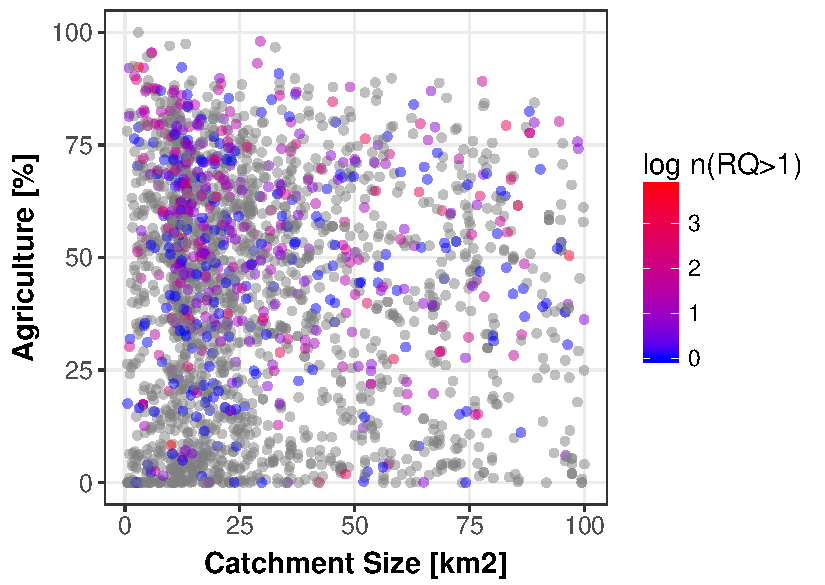
\includegraphics[width = \textwidth]{appendix/smallstreams/one/ezgagrirac}
	\caption[Raw data used for the model in equation 2 and Figure 3 of the main article.]{Raw data used for the model in equation 2 and Figure 3 of the main article. Color codes the number of RAC exceedances (on a log-scale). Grey points denote sites without any exceedance.}
	\label{fig:ezgagrirac}
\end{figure}



%% -------------------------------------------------------------------------
\clearpage
\section{Effect of precipitation and season on RQ}

\begin{figure}[H]
	\centering
	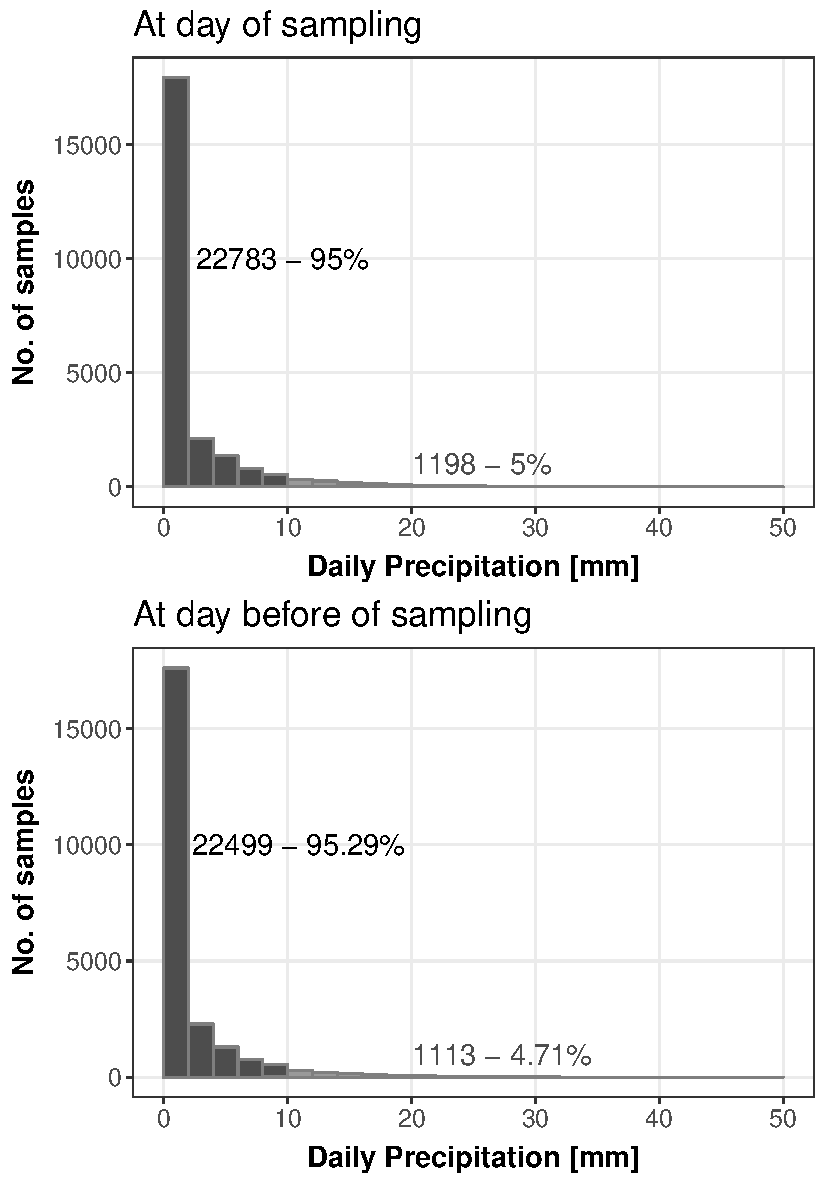
\includegraphics[width = 0.8\textwidth]{appendix/smallstreams/one/precip}
	\caption[Distribution of precipitation at sampling occasions.]{Distribution of precipitation at sampling occasions. top: at sampling date. bottom: at the day before sampling.}
	\label{fig:precip}
\end{figure}

%%% from do_precip.R
% 
\clearpage
\begin{longtable}{lp{2.5cm}rlp{1.5cm}p{1.5cm}p{1.5cm}}
\caption[23 pesticides for which we modelled the relationship with precipitation and seasonality.]{23 pesticides for which we modelled the relationship between RQ and precipitation and seasonality, respectively.
                    Order is the same as in Figure 5 of the main text. See Table \ref{tab:var_model_coef} for model coefficients.} \\ 
  \toprule
 & Name & CAS & Group & \%>LOQ & no. > LOQ & total no. \\ 
  \midrule
1 & Azoxystrobin & 131860-33-8 & fungicide & 9.58 & 644 & 6723 \\ 
  2 & Bentazon & 25057-89-0 & herbicide & 19.43 & 2313 & 11905 \\ 
  3 & Boscalid & 188425-85-6 & fungicide & 23.00 & 2175 & 9455 \\ 
  4 & Carbendazim & 10605-21-7 & fungicide & 16.10 & 582 & 3615 \\ 
  5 & Chlorpyrifos & 2921-88-2 & insecticide & 6.17 & 865 & 14026 \\ 
  6 & Clothianidin & 210880-92-5 & insecticide & 6.30 & 141 & 2237 \\ 
  7 & Diflufenican & 83164-33-4 & herbicide & 12.63 & 1867 & 14784 \\ 
  8 & Dimoxystrobin & 149961-52-4 & fungicide & 6.83 & 216 & 3164 \\ 
  9 & Diuron & 330-54-1 & herbicide & 12.07 & 2138 & 17708 \\ 
  10 & Ethofumesat & 26225-79-6 & herbicide & 5.10 & 998 & 19552 \\ 
  11 & Flufenacet & 142459-58-3 & herbicide & 5.97 & 772 & 12923 \\ 
  12 & Glyphosate & 1071-83-6 & herbicide & 40.73 & 1389 & 3410 \\ 
  13 & Imidacloprid & 138261-41-3 & insecticide & 5.88 & 176 & 2992 \\ 
  14 & Isoproturon & 34123-59-6 & herbicide & 21.84 & 3984 & 18239 \\ 
  15 & MCPA & 94-74-6 & herbicide & 12.81 & 1567 & 12237 \\ 
  16 & Mecoprop & 93-65-2 & herbicide & 12.21 & 1463 & 11984 \\ 
  17 & Metazachlor & 67129-08-2 & herbicide & 9.23 & 1930 & 20907 \\ 
  18 & Nicosulfuron & 111991-09-4 & herbicide & 5.33 & 263 & 4934 \\ 
  19 & Propiconazol & 60207-90-1 & fungicide & 5.67 & 772 & 13622 \\ 
  20 & Quinmerac & 90717-03-6 & herbicide & 13.46 & 939 & 6974 \\ 
  21 & Tebuconazol & 107534-96-3 & fungicide & 6.08 & 968 & 15924 \\ 
  22 & Terbuthylazin & 5915-41-3 & herbicide & 14.59 & 3142 & 21540 \\ 
   \bottomrule
\label{tab:var_model}
\end{longtable}

\clearpage
\begin{landscape}
\begingroup\fontsize{8pt}{10pt}\selectfont
\begin{longtable}{lp{2cm}p{0.6cm}p{1.8cm}p{1.8cm}p{1.8cm}p{1.8cm}p{1.8cm}p{1.8cm}}
\caption[Coefficients and CI from per compound models.]{Coefficients and CI from per compound models. 
                     Bold values denote coefficients where the CI for precipitation encompasses zero.
                     Coefficients are on the link scale (log for $\mu$ and logit for $\nu$).} \\ 
  \toprule
 & Compound & effect & $log~precip_0$ & $log~precip_{-1}$ & Quarter 1 & Quarter 2 & Quarter 3 & Quarter 4 \\ 
  \midrule
  \endfirsthead
  %
  \caption*{\raggedright Table \thetable\ Continued. }\\
  \toprule
 & Compound & effect & $log~precip_0$ & $log~precip_{-1}$ & Quarter 1 & Quarter 2 & Quarter 3 & Quarter 4 \\ 
  \midrule
  \endhead
%
1 & Azoxystrobin & $\mu$ & \textbf{0.23}\newline (0.15 - 0.31) & 0.04\newline (-0.03 - 0.12) & -3.39\newline (-3.56 - -3.22) & -3.02\newline (-3.14 - -2.89) & -3.16\newline (-3.29 - -3.03) & -3.47\newline (-3.63 - -3.3) \\ 
  2 & Bentazon & $\mu$ & -0.03\newline (-0.07 - 0) & 0.02\newline (-0.02 - 0.05) & -9.46\newline (-9.53 - -9.38) & -8.97\newline (-9.02 - -8.92) & -9.14\newline (-9.2 - -9.07) & -9.46\newline (-9.53 - -9.39) \\ 
  3 & Boscalid & $\mu$ & \textbf{0.06}\newline (0.02 - 0.1) & \textbf{0.1}\newline (0.06 - 0.13) & -6.72\newline (-6.79 - -6.64) & -6.42\newline (-6.49 - -6.36) & -6.51\newline (-6.58 - -6.45) & -6.58\newline (-6.65 - -6.5) \\ 
  4 & Carbendazim & $\mu$ & \textbf{-0.1}\newline (-0.16 - -0.03) & \textbf{0.16}\newline (0.09 - 0.22) & -2.42\newline (-2.58 - -2.27) & -1.95\newline (-2.05 - -1.84) & -2.11\newline (-2.22 - -2) & -2.32\newline (-2.46 - -2.18) \\ 
  5 & Chlorpyrifos & $\mu$ & \textbf{0.08}\newline (0.04 - 0.13) & -0.03\newline (-0.08 - 0.01) & 0.85\newline (0.77 - 0.93) & 1\newline (0.93 - 1.06) & 0.9\newline (0.82 - 0.98) & 0.94\newline (0.86 - 1.03) \\ 
  6 & Clothianidin & $\mu$ & 0.08\newline (-0.04 - 0.19) & -0.1\newline (-0.21 - 0.02) & 0.94\newline (0.77 - 1.12) & 0.67\newline (0.49 - 0.84) & 1.02\newline (0.8 - 1.25) & 1.55\newline (1.32 - 1.78) \\ 
  7 & Diflufenican & $\mu$ & -0.02\newline (-0.06 - 0.02) & \textbf{0.05}\newline (0.02 - 0.09) & -0.56\newline (-0.62 - -0.5) & -1.01\newline (-1.07 - -0.94) & -1.08\newline (-1.16 - -1) & -0.71\newline (-0.77 - -0.65) \\ 
  8 & Dimoxystrobin & $\mu$ & \textbf{0.35}\newline (0.2 - 0.5) & 0.02\newline (-0.15 - 0.19) & -1.17\newline (-1.44 - -0.89) & -0.42\newline (-0.64 - -0.2) & -0.07\newline (-0.39 - 0.25) & -0.02\newline (-0.35 - 0.31) \\ 
  9 & Diuron & $\mu$ & 0\newline (-0.03 - 0.03) & \textbf{0.07}\newline (0.04 - 0.1) & -2.72\newline (-2.83 - -2.61) & -2.43\newline (-2.47 - -2.39) & -2.48\newline (-2.53 - -2.44) & -2.64\newline (-2.71 - -2.58) \\ 
  10 & Ethofumesat & $\mu$ & \textbf{0.12}\newline (0.06 - 0.17) & 0.01\newline (-0.05 - 0.06) & -6.11\newline (-6.27 - -5.96) & -5.49\newline (-5.56 - -5.42) & -6.18\newline (-6.29 - -6.08) & -6.1\newline (-6.24 - -5.95) \\ 
  11 & Flufenacet & $\mu$ & 0.03\newline (-0.02 - 0.08) & \textbf{0.05}\newline (0.01 - 0.1) & -3.71\newline (-3.79 - -3.62) & -3.7\newline (-3.81 - -3.59) & -3.29\newline (-3.44 - -3.15) & -3.63\newline (-3.68 - -3.57) \\ 
  12 & Glyphosate & $\mu$ & -0.04\newline (-0.09 - 0.01) & \textbf{0.14}\newline (0.09 - 0.19) & -6.3\newline (-6.46 - -6.13) & -6.08\newline (-6.16 - -6) & -5.73\newline (-5.8 - -5.66) & -6.11\newline (-6.21 - -6.01) \\ 
  13 & Imidacloprid & $\mu$ & 0\newline (-0.08 - 0.09) & -0.01\newline (-0.09 - 0.07) & 0.61\newline (0.33 - 0.88) & 1.15\newline (1.02 - 1.27) & 1.4\newline (1.28 - 1.53) & 1.24\newline (1.06 - 1.42) \\ 
  14 & Isoproturon & $\mu$ & 0.02\newline (-0.02 - 0.05) & \textbf{0.21}\newline (0.17 - 0.24) & -3.29\newline (-3.37 - -3.22) & -3.01\newline (-3.06 - -2.96) & -3.43\newline (-3.5 - -3.35) & -2.79\newline (-2.84 - -2.73) \\ 
  15 & MCPA & $\mu$ & 0.04\newline (-0.01 - 0.09) & \textbf{0.09}\newline (0.04 - 0.14) & -5.07\newline (-5.27 - -4.87) & -4.25\newline (-4.32 - -4.19) & -4.48\newline (-4.57 - -4.4) & -4.7\newline (-4.81 - -4.58) \\ 
  16 & Mecoprop & $\mu$ & 0.04\newline (-0.01 - 0.09) & \textbf{0.05}\newline (0.01 - 0.1) & -8.36\newline (-8.49 - -8.22) & -7.59\newline (-7.65 - -7.52) & -7.77\newline (-7.85 - -7.69) & -8.07\newline (-8.18 - -7.97) \\ 
  17 & Metazachlor & $\mu$ & \textbf{-0.07}\newline (-0.12 - -0.02) & \textbf{0.09}\newline (0.04 - 0.13) & -2.97\newline (-3.06 - -2.88) & -2.94\newline (-3.04 - -2.85) & -2.21\newline (-2.28 - -2.14) & -2.77\newline (-2.84 - -2.7) \\ 
  18 & Nicosulfuron & $\mu$ & \textbf{0.23}\newline (0.12 - 0.34) & \textbf{-0.28}\newline (-0.39 - -0.18) & -0.98\newline (-1.22 - -0.74) & -0.2\newline (-0.36 - -0.03) & -0.07\newline (-0.25 - 0.11) & -0.97\newline (-1.16 - -0.78) \\ 
  19 & Propiconazol & $\mu$ & \textbf{0.08}\newline (0.02 - 0.14) & 0.01\newline (-0.05 - 0.07) & -3.99\newline (-4.15 - -3.83) & -3.63\newline (-3.71 - -3.55) & -3.82\newline (-3.91 - -3.72) & -3.63\newline (-3.74 - -3.53) \\ 
  20 & Quinmerac & $\mu$ & 0.02\newline (-0.05 - 0.09) & 0.05\newline (-0.01 - 0.12) & -9.08\newline (-9.19 - -8.96) & -9.12\newline (-9.24 - -9) & -8.46\newline (-8.59 - -8.33) & -8.64\newline (-8.72 - -8.55) \\ 
  21 & Tebuconazol & $\mu$ & -0.01\newline (-0.06 - 0.03) & \textbf{0.09}\newline (0.04 - 0.14) & -2.17\newline (-2.28 - -2.06) & -1.93\newline (-2 - -1.86) & -2.2\newline (-2.28 - -2.11) & -2.15\newline (-2.24 - -2.06) \\ 
  22 & Terbuthylazin & $\mu$ & \textbf{0.09}\newline (0.06 - 0.13) & \textbf{0.11}\newline (0.08 - 0.15) & -3.65\newline (-3.73 - -3.56) & -2.78\newline (-2.84 - -2.73) & -3.25\newline (-3.3 - -3.19) & -3.52\newline (-3.59 - -3.44) \\ 
   \midrule
23 & Azoxystrobin & $\nu$ & 0\newline (-0.13 - 0.13) & \textbf{0.24}\newline (0.11 - 0.37) & -3.5\newline (-3.76 - -3.25) & -2.33\newline (-2.54 - -2.13) & -2.14\newline (-2.36 - -1.92) & -3.2\newline (-3.45 - -2.95) \\ 
  24 & Bentazon & $\nu$ & 0\newline (-0.08 - 0.08) & 0.05\newline (-0.03 - 0.13) & -2.26\newline (-2.44 - -2.09) & -1.53\newline (-1.65 - -1.4) & -1.88\newline (-2.02 - -1.74) & -2.25\newline (-2.4 - -2.11) \\ 
  25 & Boscalid & $\nu$ & -0.01\newline (-0.1 - 0.08) & \textbf{0.45}\newline (0.37 - 0.54) & -1.99\newline (-2.16 - -1.82) & -1.22\newline (-1.36 - -1.07) & -1.24\newline (-1.38 - -1.09) & -1.81\newline (-1.96 - -1.65) \\ 
  26 & Carbendazim & $\nu$ & 0.09\newline (-0.04 - 0.22) & \textbf{0.19}\newline (0.06 - 0.32) & -2.72\newline (-3 - -2.44) & -1.49\newline (-1.69 - -1.28) & -1.26\newline (-1.48 - -1.04) & -2.31\newline (-2.56 - -2.06) \\ 
  27 & Chlorpyrifos & $\nu$ & \textbf{0.11}\newline (0.01 - 0.21) & 0.1\newline (0 - 0.19) & -3.27\newline (-3.45 - -3.1) & -2.63\newline (-2.79 - -2.48) & -3.22\newline (-3.39 - -3.05) & -3.42\newline (-3.61 - -3.23) \\ 
  28 & Clothianidin & $\nu$ & -0.05\newline (-0.3 - 0.2) & 0.19\newline (-0.07 - 0.44) & -2.66\newline (-3.06 - -2.26) & -2.58\newline (-2.97 - -2.19) & -3.19\newline (-3.69 - -2.69) & -3.93\newline (-4.46 - -3.41) \\ 
  29 & Diflufenican & $\nu$ & 0.06\newline (-0.02 - 0.14) & \textbf{0.26}\newline (0.17 - 0.34) & -1.89\newline (-2.03 - -1.75) & -2.45\newline (-2.59 - -2.31) & -3.14\newline (-3.3 - -2.98) & -2.09\newline (-2.22 - -1.95) \\ 
  30 & Dimoxystrobin & $\nu$ & 0.19\newline (-0.02 - 0.41) & \textbf{0.23}\newline (0.01 - 0.46) & -3.37\newline (-3.78 - -2.96) & -2.25\newline (-2.58 - -1.91) & -3.14\newline (-3.55 - -2.72) & -3.58\newline (-4.02 - -3.15) \\ 
  31 & Diuron & $\nu$ & 0.05\newline (-0.01 - 0.12) & \textbf{0.28}\newline (0.22 - 0.35) & -3.88\newline (-4.09 - -3.67) & -1.67\newline (-1.76 - -1.58) & -1.74\newline (-1.84 - -1.63) & -2.72\newline (-2.85 - -2.6) \\ 
  32 & Ethofumesat & $\nu$ & 0.09\newline (-0.01 - 0.18) & \textbf{0.21}\newline (0.12 - 0.3) & -4.39\newline (-4.63 - -4.16) & -2.23\newline (-2.35 - -2.11) & -3.49\newline (-3.66 - -3.32) & -4.23\newline (-4.44 - -4.01) \\ 
  33 & Flufenacet & $\nu$ & \textbf{0.16}\newline (0.06 - 0.27) & \textbf{0.59}\newline (0.49 - 0.69) & -2.57\newline (-2.75 - -2.39) & -3.8\newline (-4.01 - -3.58) & -4.17\newline (-4.44 - -3.89) & -1.76\newline (-1.88 - -1.64) \\ 
  34 & Glyphosate & $\nu$ & 0.11\newline (0 - 0.23) & \textbf{0.29}\newline (0.18 - 0.4) & -1.79\newline (-2.09 - -1.48) & -0.12\newline (-0.3 - 0.05) & 0.34\newline (0.17 - 0.51) & -0.53\newline (-0.73 - -0.32) \\ 
  35 & Imidacloprid & $\nu$ & -0.01\newline (-0.26 - 0.25) & -0.1\newline (-0.34 - 0.15) & -4.68\newline (-5.35 - -4) & -3.04\newline (-3.41 - -2.68) & -2.83\newline (-3.21 - -2.45) & -4.07\newline (-4.56 - -3.58) \\ 
  36 & Isoproturon & $\nu$ & 0.04\newline (-0.02 - 0.09) & \textbf{0.31}\newline (0.25 - 0.36) & -1.82\newline (-1.93 - -1.7) & -1.19\newline (-1.27 - -1.12) & -2.11\newline (-2.22 - -2.01) & -0.8\newline (-0.88 - -0.72) \\ 
  37 & MCPA & $\nu$ & -0.06\newline (-0.13 - 0.02) & \textbf{0.35}\newline (0.28 - 0.42) & -3.79\newline (-4.04 - -3.54) & -1.27\newline (-1.37 - -1.18) & -1.81\newline (-1.93 - -1.68) & -2.77\newline (-2.92 - -2.62) \\ 
  38 & Mecoprop & $\nu$ & 0.07\newline (-0.01 - 0.15) & \textbf{0.35}\newline (0.27 - 0.42) & -3.04\newline (-3.23 - -2.84) & -1.56\newline (-1.67 - -1.45) & -1.89\newline (-2.02 - -1.76) & -2.71\newline (-2.86 - -2.56) \\ 
  39 & Metazachlor & $\nu$ & 0.06\newline (-0.01 - 0.13) & \textbf{0.21}\newline (0.14 - 0.27) & -2.81\newline (-2.94 - -2.67) & -3.22\newline (-3.36 - -3.09) & -2.11\newline (-2.22 - -2.01) & -2.05\newline (-2.16 - -1.95) \\ 
  40 & Nicosulfuron & $\nu$ & \textbf{0.2}\newline (0.01 - 0.39) & \textbf{0.26}\newline (0.07 - 0.45) & -3.87\newline (-4.27 - -3.48) & -2.96\newline (-3.26 - -2.66) & -2.99\newline (-3.3 - -2.68) & -3.23\newline (-3.56 - -2.9) \\ 
  41 & Propiconazol & $\nu$ & -0.02\newline (-0.13 - 0.09) & \textbf{0.39}\newline (0.29 - 0.5) & -4.05\newline (-4.32 - -3.78) & -2.72\newline (-2.88 - -2.57) & -2.88\newline (-3.06 - -2.7) & -3.43\newline (-3.63 - -3.24) \\ 
  42 & Quinmerac & $\nu$ & -0.03\newline (-0.13 - 0.08) & \textbf{0.32}\newline (0.22 - 0.42) & -2.23\newline (-2.43 - -2.02) & -2.58\newline (-2.76 - -2.41) & -2.49\newline (-2.69 - -2.29) & -1.2\newline (-1.34 - -1.06) \\ 
  43 & Tebuconazol & $\nu$ & \textbf{0.1}\newline (0.01 - 0.2) & \textbf{0.3}\newline (0.21 - 0.39) & -3.41\newline (-3.61 - -3.2) & -2.66\newline (-2.8 - -2.53) & -2.9\newline (-3.06 - -2.75) & -3.17\newline (-3.34 - -3) \\ 
  44 & Terbuthylazin & $\nu$ & \textbf{0.06}\newline (0.01 - 0.12) & \textbf{0.28}\newline (0.22 - 0.33) & -2.92\newline (-3.05 - -2.79) & -1.45\newline (-1.53 - -1.37) & -1.48\newline (-1.57 - -1.39) & -2.47\newline (-2.58 - -2.37) \\ 
   \bottomrule
\label{tab:var_model_coef}
\end{longtable}
\endgroup
\end{landscape}


\begin{figure}
	\centering
	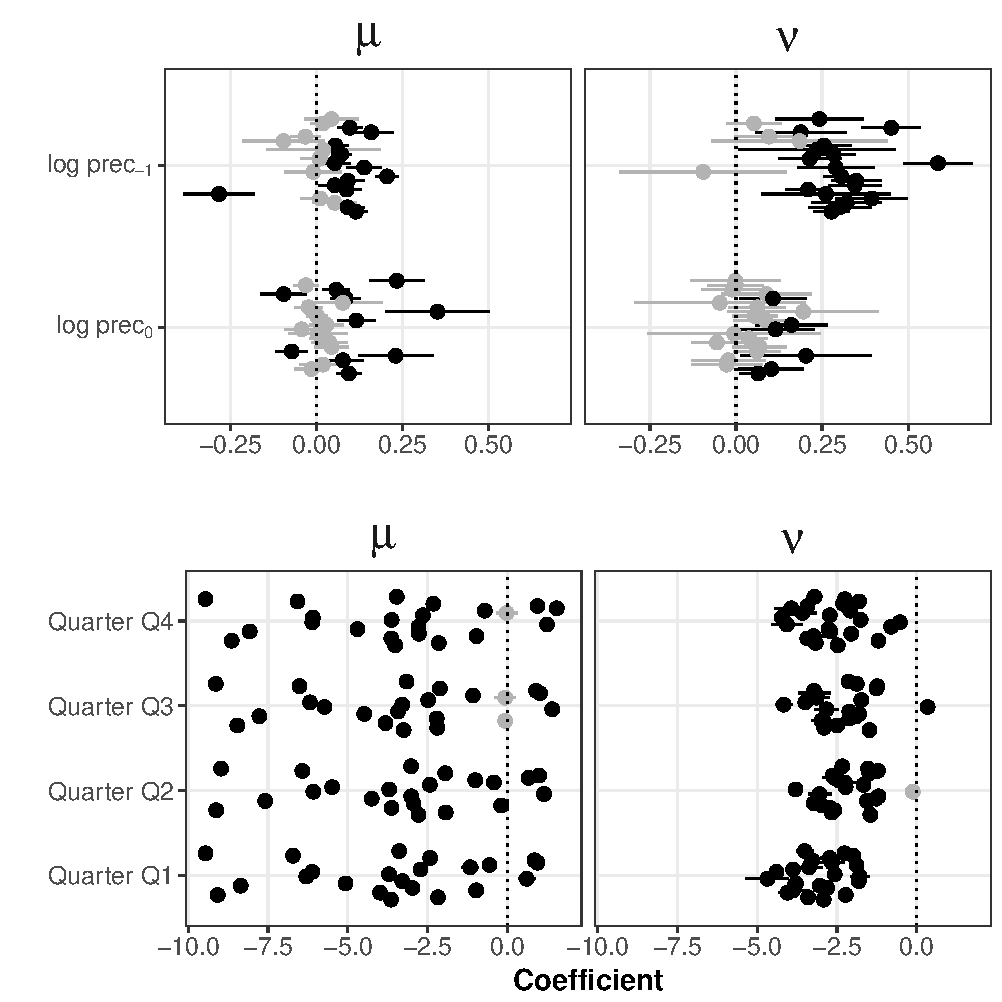
\includegraphics[width = 0.95\textwidth]{appendix/smallstreams/one/coefs}
	\caption[Graphical representation of coefficients from table \ref{tab:var_model_coef}.]{Graphical representation of coefficients from table \ref{tab:var_model_coef}. Top row: Effect of precipitation at the day before sampling and at day of sampling. Bottom row: estimates for the four Quarters. Each dot represents one compound (in the order described in table \ref{tab:var_model}). Coefficients where the CI encompasses zero are shown in gray colour. Coefficients are shown on the link scale (log for $\mu$ and logit for $\nu$).}
	\label{fig:coefs}
\end{figure}
% 


%% -------------------------------------------------------------------------
\clearpage
\section{Pesticides in small streams}
%% from do_pollution.R
\vspace{-0.5cm}
\begin{longtable}{p{2.5cm}rR{1cm}R{1cm}R{1.2cm}R{1.2cm}R{1.3cm}}
\caption[Overview on RAC exceedances of the 78 compounds with more than 1000 measurements.]{Overview on RAC exceedances of the 78 compounds with more than 1000 measurements. No. = number of measurements;  \% RQ \textgreater 1 = RAC exceedances; \% RQ \textgreater 1 | \textgreater LOQ= RAC exceedances as fraction of detects.} \\ 
  \toprule
Name & No.  & No. \textgreater LOQ & \% \textgreater LOQ & No. RQ \textgreater 1 & \% RQ \textgreater 1 & \% RQ \textgreater 1 | \textgreater LOQ \\ 
  \midrule
  \endfirsthead
  %
\caption*{\raggedright Table \thetable\ Continued. }\\
\toprule
Name & No.  & No. \textgreater LOQ & \% \textgreater LOQ & No. RQ \textgreater 1 & \% RQ \textgreater 1 & \% RQ \textgreater 1 | \textgreater LOQ \\ 
\midrule
\endhead
%
2,4-D & 12290 & 284 & 2.3 & 10 & 0.1 & 3.5 \\ 
  Aclonifen & 9861 & 67 & 0.7 &  4 & 0.0 & 6.0 \\ 
  Azoxystrobin & 7059 & 690 & 9.8 &  6 & 0.1 & 0.9 \\ 
  Benalaxyl & 6964 & 10 & 0.1 &  0 & 0.0 & 0.0 \\ 
  Bentazon & 12429 & 2421 & 19.5 &  0 & 0.0 & 0.0 \\ 
  Bifenthrin & 1353 &  0 & 0.0 &  0 & 0.0 &  \\ 
  Boscalid & 9886 & 2296 & 23.2 &  0 & 0.0 & 0.0 \\ 
  Bromoxynil & 9451 & 78 & 0.8 &  0 & 0.0 & 0.0 \\ 
  Carbendazim & 3851 & 654 & 17.0 & 12 & 0.3 & 1.8 \\ 
  Chloridazon & 15724 & 511 & 3.2 &  0 & 0.0 & 0.0 \\ 
  Chlorpyrifos & 14704 & 954 & 6.5 & 838 & 5.7 & 87.8 \\ 
  Chlortoluron & 18286 & 371 & 2.0 &  2 & 0.0 & 0.5 \\ 
  Clomazon & 9268 & 440 & 4.7 &  0 & 0.0 & 0.0 \\ 
  Clopyralid & 5520 & 107 & 1.9 &  0 & 0.0 & 0.0 \\ 
  Clothianidin & 2409 & 154 & 6.4 & 123 & 5.1 & 79.9 \\ 
  Cypermetryn & 1428 &  5 & 0.4 &  1 & 0.1 & 20.0 \\ 
  Cyprodinil & 9779 & 118 & 1.2 &  0 & 0.0 & 0.0 \\ 
  Dicamba & 7641 & 76 & 1.0 &  0 & 0.0 & 0.0 \\ 
  Difenoconazol & 1644 & 11 & 0.7 &  2 & 0.1 & 18.2 \\ 
  Diflufenican & 15457 & 1932 & 12.5 & 273 & 1.8 & 14.1 \\ 
  Dimefuron & 7833 &  5 & 0.1 &  0 & 0.0 & 0.0 \\ 
  Dimethachlor & 8858 & 344 & 3.9 &  0 & 0.0 & 0.0 \\ 
  Dimethoat & 14423 & 185 & 1.3 &  1 & 0.0 & 0.5 \\ 
  Dimethomorph & 2316 & 91 & 3.9 &  0 & 0.0 & 0.0 \\ 
  Dimoxystrobin & 3370 & 232 & 6.9 & 49 & 1.5 & 21.1 \\ 
  Diuron & 18560 & 2336 & 12.6 & 40 & 0.2 & 1.7 \\ 
  Epoxiconazol & 16454 & 621 & 3.8 &  7 & 0.0 & 1.1 \\ 
  Ethofumesat & 20430 & 1078 & 5.3 &  0 & 0.0 & 0.0 \\ 
  Fenhexamid & 2690 & 42 & 1.6 &  0 & 0.0 & 0.0 \\ 
  Fenpropimorph & 12850 & 199 & 1.5 &  5 & 0.0 & 2.5 \\ 
  Fluazifop & 3022 & 57 & 1.9 &  0 & 0.0 & 0.0 \\ 
  Fluazifop-P & 4033 & 14 & 0.3 &  0 & 0.0 & 0.0 \\ 
  Fluazifop-P-butyl & 1728 &  0 & 0.0 &  0 & 0.0 &  \\ 
  Fluazifop-butyl & 1287 &  0 & 0.0 &  0 & 0.0 &  \\ 
  Fludioxonil & 3203 & 42 & 1.3 &  1 & 0.0 & 2.4 \\ 
  Flufenacet & 13509 & 798 & 5.9 &  1 & 0.0 & 0.1 \\ 
  Fluquinconazole & 6762 & 117 & 1.7 &  0 & 0.0 & 0.0 \\ 
  Fluroxypyr & 8096 & 378 & 4.7 &  0 & 0.0 & 0.0 \\ 
  Flurtamone & 16958 & 638 & 3.8 &  2 & 0.0 & 0.3 \\ 
  Flusilazol & 5257 & 53 & 1.0 &  1 & 0.0 & 1.9 \\ 
  Glyphosate & 3557 & 1455 & 40.9 &  1 & 0.0 & 0.1 \\ 
  Imidacloprid & 3169 & 192 & 6.1 & 169 & 5.3 & 88.0 \\ 
  Ioxynil & 8114 & 20 & 0.2 &  0 & 0.0 & 0.0 \\ 
  Isoproturon & 19112 & 4164 & 21.8 & 92 & 0.5 & 2.2 \\ 
  Kresoxim-methyl & 6929 & 14 & 0.2 &  0 & 0.0 & 0.0 \\ 
  Lenacil & 13837 & 183 & 1.3 &  0 & 0.0 & 0.0 \\ 
  MCPA & 12773 & 1687 & 13.2 &  2 & 0.0 & 0.1 \\ 
  Mecoprop & 12521 & 1552 & 12.4 &  0 & 0.0 & 0.0 \\ 
  Metalaxyl & 14460 & 299 & 2.1 &  0 & 0.0 & 0.0 \\ 
  Metamitron & 15390 & 613 & 4.0 &  0 & 0.0 & 0.0 \\ 
  Metazachlor & 21906 & 2015 & 9.2 & 55 & 0.3 & 2.7 \\ 
  Methamidophos & 1303 &  0 & 0.0 &  0 & 0.0 &  \\ 
  Methobromuron & 14968 & 24 & 0.2 &  1 & 0.0 & 4.2 \\ 
  Metribuzin & 15411 & 192 & 1.2 & 15 & 0.1 & 7.8 \\ 
  Napropamid & 9914 & 269 & 2.7 &  1 & 0.0 & 0.4 \\ 
  Nicosulfuron & 5172 & 288 & 5.6 & 77 & 1.5 & 26.7 \\ 
  Penconazol & 4846 & 159 & 3.3 &  0 & 0.0 & 0.0 \\ 
  Pendimethalin & 16997 & 328 & 1.9 &  4 & 0.0 & 1.2 \\ 
  Pethoxamid & 3102 & 37 & 1.2 &  0 & 0.0 & 0.0 \\ 
  Phoxim & 1492 &  0 & 0.0 &  0 & 0.0 &  \\ 
  Picolinafen & 8901 & 11 & 0.1 &  2 & 0.0 & 18.2 \\ 
  Picoxystrobin & 3620 &  7 & 0.2 &  0 & 0.0 & 0.0 \\ 
  Pirimicarb & 11330 & 232 & 2.0 & 27 & 0.2 & 11.6 \\ 
  Prochloraz & 5795 & 33 & 0.6 &  0 & 0.0 & 0.0 \\ 
  Propiconazol & 14250 & 818 & 5.7 &  7 & 0.0 & 0.9 \\ 
  Propyzamid & 11937 & 453 & 3.8 &  0 & 0.0 & 0.0 \\ 
  Prosulfocarb & 5001 & 126 & 2.5 &  0 & 0.0 & 0.0 \\ 
  Pyrimethanil & 8136 & 122 & 1.5 &  0 & 0.0 & 0.0 \\ 
  Quinmerac & 7291 & 989 & 13.6 &  0 & 0.0 & 0.0 \\ 
  Rimsulfuron & 1240 &  2 & 0.2 &  0 & 0.0 & 0.0 \\ 
  Spiroxamin & 2469 & 109 & 4.4 &  1 & 0.0 & 0.9 \\ 
  Tebuconazol & 16584 & 1024 & 6.2 & 26 & 0.2 & 2.5 \\ 
  Terbuthylazin & 22568 & 3370 & 14.9 & 35 & 0.2 & 1.0 \\ 
  Thiacloprid & 3540 & 85 & 2.4 & 85 & 2.4 & 100.0 \\ 
  Thiamethoxam & 1853 & 39 & 2.1 &  7 & 0.4 & 17.9 \\ 
  Triadimenol & 3067 & 51 & 1.7 &  0 & 0.0 & 0.0 \\ 
  Triazophos & 3588 &  2 & 0.1 &  1 & 0.0 & 50.0 \\ 
  Trifloxystrobin & 3674 & 10 & 0.3 &  1 & 0.0 & 10.0 \\
   \bottomrule
\label{tab:rac_dat}
\end{longtable}


\begin{figure}[ht]
	\centering
	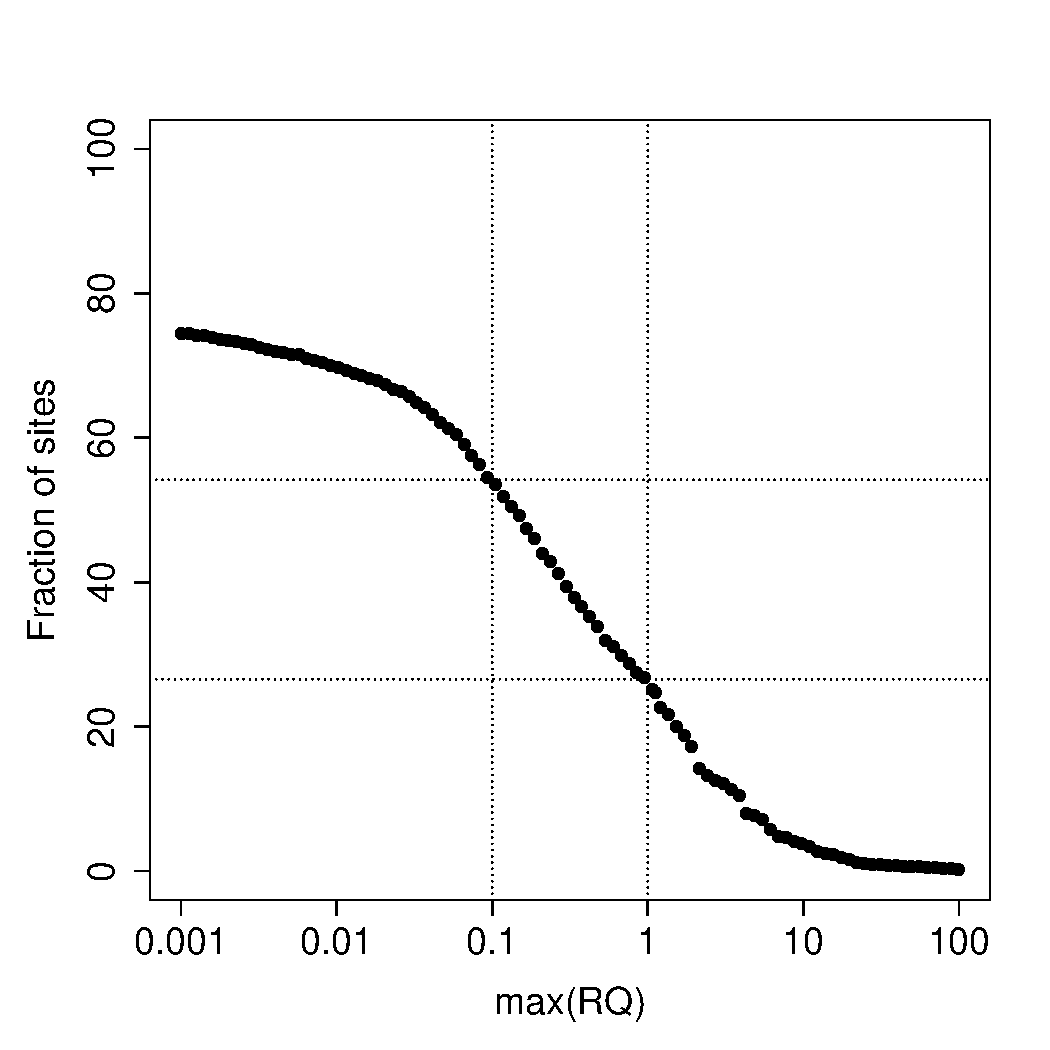
\includegraphics[width = 0.8\textwidth]{appendix/smallstreams/one/prac_ex}
	\caption[Cumulative distribution of the number sites exceeding RAC.]{Cumulative distribution of sites exceeding RAC. Dotted lines indicate fraction of sites exceeding a RQ of 1 and 0.1. 23\% of the sites showed no detection of compounds with available RAC values and are not shown due to logarithmic x-axis.}
	\label{fig:prac_ex}
\end{figure}


\begin{landscape}
\begin{figure}[ht]
	\centering
	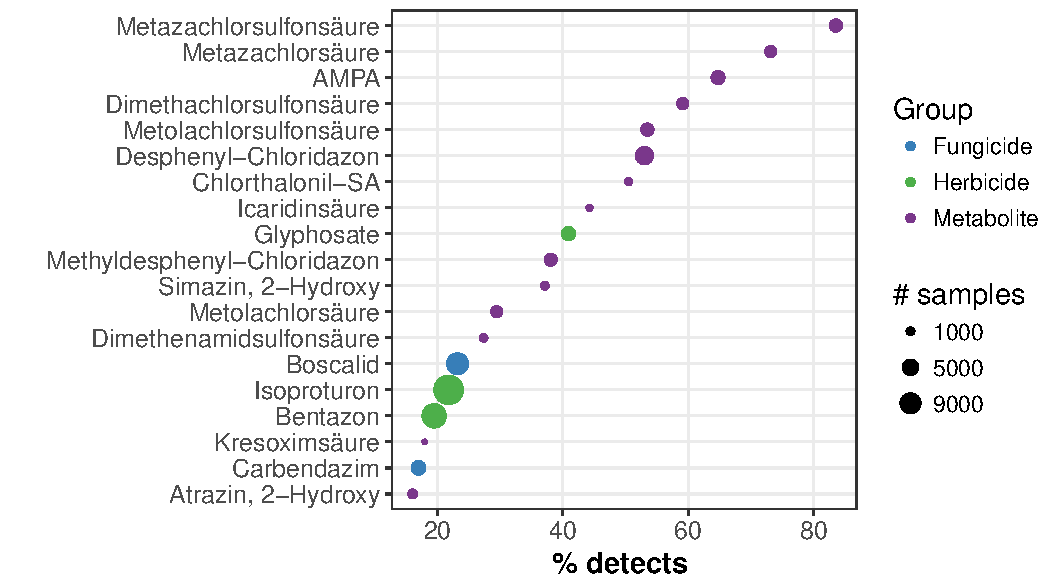
\includegraphics[width = 0.8\textheight]{appendix/smallstreams/one/pdetects}
	\caption[Proportion of samples with detects in small streams.]{Proportion of samples with detects in small streams. Only Compounds with more than 100 samples and 15\% of detects are shown.}
	\label{fig:pdetects}
\end{figure}
\end{landscape}

\begin{figure}[ht]
	\centering
	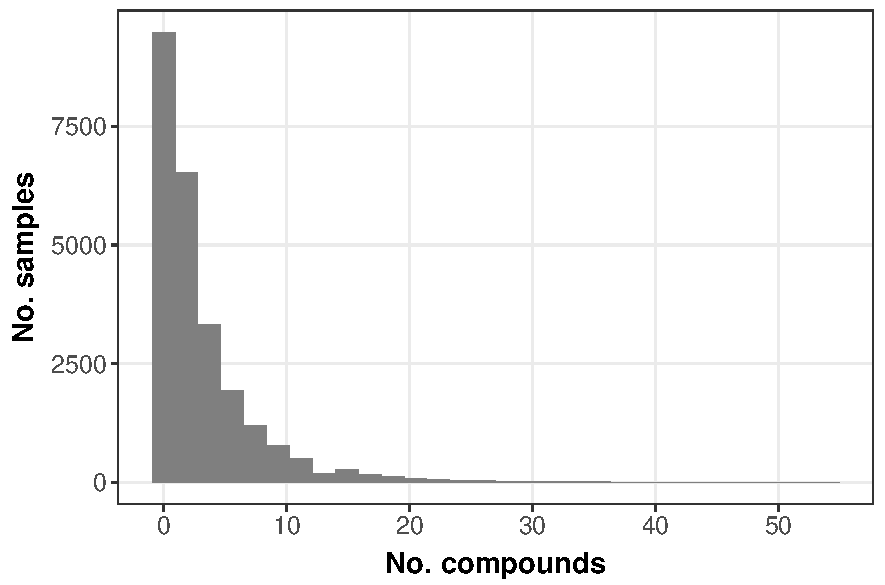
\includegraphics[width = 0.9\textwidth]{appendix/smallstreams/one/pmix}
	\caption{Distribution of the number of quantified compounds in the samples.}
	\label{fig:pmix}
\end{figure}


\clearpage
\section{Catchment size - stream width relationship}
We studied the relationship between catchment size based on three datasets containing this informations:
Data delivered by the federal state Thuringia, \citet{vos_organic_2015} and \citet{fernandez_effects_2015} (both from Rhineland-Palatinate).
We fitted to each dataset separately and to the combined dataset a power-function.
The resulting models are shown in Figure \ref{fig:size_width}. 

\begin{figure}[ht]
	\centering
	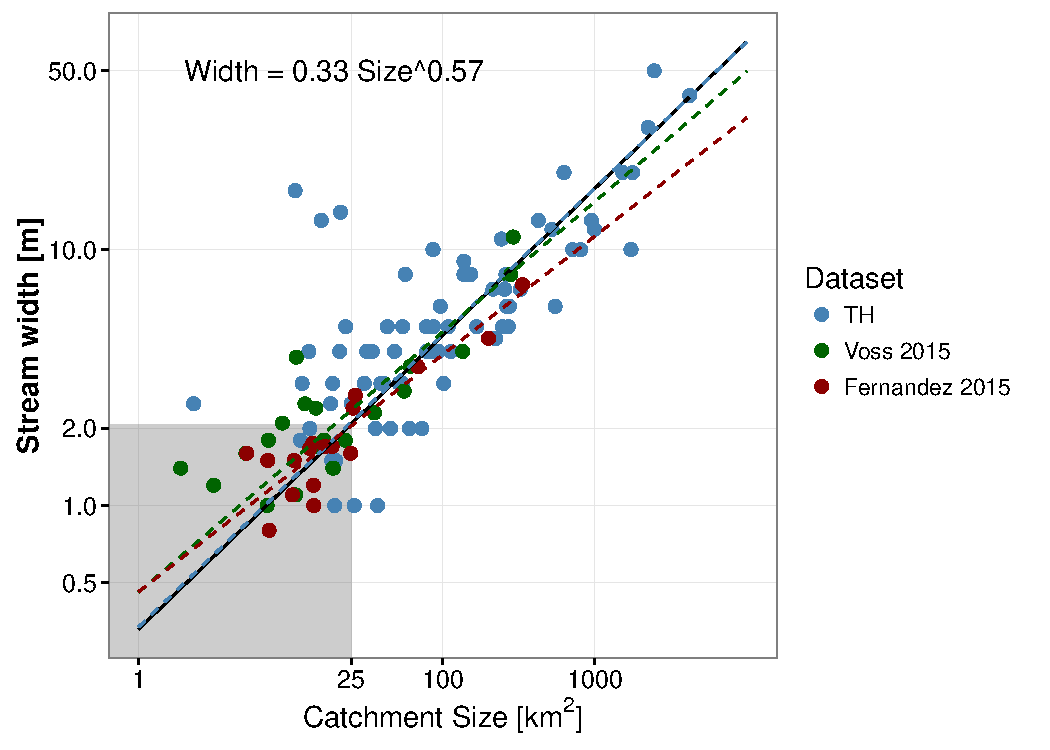
\includegraphics[width = 0.9\textwidth]{appendix/smallstreams/one/width_size}
		\caption[Relationship between catchment size and stream width.]{Relationship between catchment size and stream width. A power function has been fitted to each dataset separately (colored dashed lines) and the combined dataset (black line and equation). The gray rectangle marks the estimated width for a catchment size of 25km\textsuperscript{2}.}
	\label{fig:size_width}
\end{figure}

\clearpage
\section{References}
\printbibliography[heading=none]



%----------------------------------------------------------------------------
% taxize
\cleardoublepage
\def\dir{appendix/taxize}
\chapter{Supplemental material for: taxize: taxonomic search and retrieval}
\addthumb{\thechapter}{\Huge\thechapter}{white}{gray}
\label{ap:taxize}  



  
\section[A complete reproducible workflow]{A complete reproducible workflow, from a species list to a phylogeny, and distribution map.} 
\label{ap:taxize:one} 

If you aren't familiar with a complete workflow in R, it may be difficult to visualize the process. In R, everything is programmatic, so the whole workflow can be in one place, and be repeated whenever necessary. The following is a workflow for taxize, going from a species list to a phylogeny. 

First, install taxize

\begin{knitrout}
\definecolor{shadecolor}{rgb}{0.969, 0.969, 0.969}\color{fgcolor}\begin{kframe}
\begin{alltt}
\hlkwd{install.packages}\hlstd{(}\hlstr{"taxize"}\hlstd{)}
\end{alltt}
\end{kframe}
\end{knitrout}


Then load it into R

\begin{knitrout}
\definecolor{shadecolor}{rgb}{0.969, 0.969, 0.969}\color{fgcolor}\begin{kframe}
\begin{alltt}
\hlkwd{library}\hlstd{(taxize)}
\end{alltt}
\end{kframe}
\end{knitrout}


Most of us will start out with a species list, something like the one below. Note that each of the names is spelled incorrectly.

\begin{knitrout}
\definecolor{shadecolor}{rgb}{0.969, 0.969, 0.969}\color{fgcolor}\begin{kframe}
\begin{alltt}
\hlstd{splist} \hlkwb{<-} \hlkwd{c}\hlstd{(}\hlstr{"Helanthus annuus"}\hlstd{,} \hlstr{"Pinos contorta"}\hlstd{,} 
         \hlstr{"Collomia grandiflorra"}\hlstd{,} \hlstr{"Rosa california"}\hlstd{,}
         \hlstr{"Mimulus bicolour"}\hlstd{,} \hlstr{"Nicotiana glauca"}\hlstd{,} \hlstr{"Maddia sativa"}\hlstd{)}
\end{alltt}
\end{kframe}
\end{knitrout}


There are many ways to resolve taxonomic names in taxize. Of course, the ideal name resolver will do the work behind the scenes for you so that you don't have to do things like fuzzy matching. There are a few services in taxize like this we can choose from: the Global Names Resolver service from EOL (see function \emph{gnr\_resolve}) and the Taxonomic Name Resolution Service from iPlant (see function \emph{tnrs}). In this case let's use the function \emph{tnrs}. 

\begin{knitrout}
\definecolor{shadecolor}{rgb}{0.969, 0.969, 0.969}\color{fgcolor}\begin{kframe}
\begin{alltt}
\hlcom{# The tnrs function accepts a vector of 1 or more}
\hlstd{splist_tnrs} \hlkwb{<-} \hlkwd{tnrs}\hlstd{(}\hlkwc{query} \hlstd{= splist,} \hlkwc{getpost} \hlstd{=} \hlstr{"POST"}\hlstd{,} 
         \hlkwc{source_} \hlstd{=} \hlstr{"iPlant_TNRS"}\hlstd{)}
\hlcom{# Remove some fields}
\hlstd{(splist_tnrs} \hlkwb{<-} \hlstd{splist_tnrs[,} \hlopt{!}\hlkwd{names}\hlstd{(splist_tnrs)} \hlopt 
         \hlkwd{c}\hlstd{(}\hlstr{"matchedName"}\hlstd{,} \hlstr{"annotations"}\hlstd{,}
    \hlstr{"uri"}\hlstd{)])}
\end{alltt}
\begin{verbatim}
#           submittedName         acceptedName    sourceId score
# 5      Helanthus annuus    Helianthus annuus iPlant_TNRS  0.98
# 1        Pinos contorta       Pinus contorta iPlant_TNRS  0.96
# 7 Collomia grandiflorra Collomia grandiflora iPlant_TNRS  0.99
# 6       Rosa california     Rosa californica iPlant_TNRS  0.99
# 4      Mimulus bicolour      Mimulus bicolor iPlant_TNRS  0.98
# 3      Nicotiana glauca     Nicotiana glauca iPlant_TNRS     1
# 2         Maddia sativa         Madia sativa iPlant_TNRS  0.97
\end{verbatim}
\begin{alltt}
\hlcom{# Note the scores. They suggest that there were no perfect matches,}
\hlcom{# but they were all very close, ranging from 0.77 to 0.99}
\hlcom{# (1 is the highest).}
\hlcom{# Let's assume the names in the 'acceptedName' column}
\hlcom{# are correct (and they should}
\hlcom{# be).}
\hlcom{# So here's our updated species list}
\hlstd{(splist} \hlkwb{<-} \hlkwd{as.character}\hlstd{(splist_tnrs}\hlopt{$}\hlstd{acceptedName))}
\end{alltt}
\begin{verbatim}
# [1] "Helianthus annuus"  "Pinus contorta"  "Collomia grandiflora"
# [4] "Rosa californica"  "Mimulus bicolor"  "Nicotiana glauca"    
# [7] "Madia sativa"
\end{verbatim}
\end{kframe}
\end{knitrout}


Another thing we may want to do is collect common names for our taxa. 

\begin{knitrout}
\definecolor{shadecolor}{rgb}{0.969, 0.969, 0.969}\color{fgcolor}\begin{kframe}
\begin{alltt}
\hlstd{tsns} \hlkwb{<-} \hlkwd{get_tsn}\hlstd{(}\hlkwc{searchterm} \hlstd{= splist,} \hlkwc{searchtype} \hlstd{=} \hlstr{"sciname"}\hlstd{,} 
        \hlkwc{verbose} \hlstd{=} \hlnum{FALSE}\hlstd{)}
\hlstd{comnames} \hlkwb{<-} \hlkwd{lapply}\hlstd{(tsns, getcommonnamesfromtsn)}
\hlcom{# Unfortunately, common names are not standardized like species}
\hlcom{# names, so there are multiple common names for each taxon}
\hlkwd{sapply}\hlstd{(comnames, length)}
\end{alltt}
\begin{verbatim}
# [1] 3 3 3 3 3 3 3
\end{verbatim}
\begin{alltt}
\hlcom{# So let's just take the first common name for each species}
\hlstd{comnames_vec} \hlkwb{<-} \hlkwd{do.call}\hlstd{(c,} \hlkwd{lapply}\hlstd{(comnames,} 
     \hlkwa{function}\hlstd{(}\hlkwc{x}\hlstd{)} \hlkwd{as.character}\hlstd{(x[}\hlnum{1}\hlstd{,} \hlstr{"comname"}\hlstd{])))}
\hlcom{# And we can make a data.frame of our scientific and common names}
\hlstd{(allnames} \hlkwb{<-} \hlkwd{data.frame}\hlstd{(}\hlkwc{spname} \hlstd{= splist,} \hlkwc{comname} \hlstd{= comnames_vec))}
\end{alltt}
\begin{verbatim}
#                 spname                       comname
# 1    Helianthus annuus              common sunflower
# 2       Pinus contorta                lodgepole pine
# 3 Collomia grandiflora        largeflowered collomia
# 4     Rosa californica           California wildrose
# 5      Mimulus bicolor yellow and white monkeyflower
# 6     Nicotiana glauca                  tree tobacco
# 7         Madia sativa                 coast tarweed
\end{verbatim}
\end{kframe}
\end{knitrout}


Another common task is getting the taxonomic tree upstream from your study taxa. We often know what family or order our taxa are in, but it we often don't know the tribes, subclasses, and superfamilies. taxize provides many avenues to getting classifications. Two of them are accessible via a single function (\emph{classification}): the Integrated Taxonomic Information System (ITIS) and National Center for Biotechnology Information (NCBI); and via the Catalogue of Life (see function \emph{col\_classification}):

\begin{knitrout}
\definecolor{shadecolor}{rgb}{0.969, 0.969, 0.969}\color{fgcolor}\begin{kframe}
\begin{alltt}
\hlcom{# As we already have Taxonomic Serial Numbers from ITIS, let's just}
\hlcom{# get classifications from ITIS.Note that we could use uBio instead.}
\hlstd{class_list} \hlkwb{<-} \hlkwd{classification}\hlstd{(tsns)}
\hlkwd{sapply}\hlstd{(class_list, nrow)}
\end{alltt}
\begin{verbatim}
# [1] 12 11 12 12 12 12 12
\end{verbatim}
\begin{alltt}
\hlcom{# And we can attach these names to our allnames data.frame}
\hlkwd{library}\hlstd{(plyr)}
\hlstd{gethiernames} \hlkwb{<-} \hlkwa{function}\hlstd{(}\hlkwc{x}\hlstd{) \{}
    \hlstd{temp} \hlkwb{<-} \hlstd{x[,} \hlkwd{c}\hlstd{(}\hlstr{"rankName"}\hlstd{,} \hlstr{"taxonName"}\hlstd{)]}
    \hlstd{values} \hlkwb{<-} \hlkwd{data.frame}\hlstd{(}\hlkwd{t}\hlstd{(temp[,} \hlnum{2}\hlstd{]))}
    \hlkwd{names}\hlstd{(values)} \hlkwb{<-} \hlstd{temp[,} \hlnum{1}\hlstd{]}
    \hlkwd{return}\hlstd{(values)}
\hlstd{\}}
\hlstd{class_df} \hlkwb{<-} \hlkwd{ldply}\hlstd{(class_list, gethiernames)}
\hlstd{allnames_df} \hlkwb{<-} \hlkwd{merge}\hlstd{(allnames, class_df,} \hlkwc{by.x} \hlstd{=} \hlstr{"spname"}\hlstd{,} 
         \hlkwc{by.y} \hlstd{=} \hlstr{"Species"}\hlstd{)}
\hlcom{# Now that we have allnames_df, we can start to see some}
\hlcom{# relationships among species simply by their shared taxonomic names}
\hlstd{allnames_df[}\hlnum{1}\hlopt{:}\hlnum{2}\hlstd{, ]}
\end{alltt}
{\small
\begin{verbatim}
#                 spname                comname Kingdom     Subkingdom
# 1 Collomia grandiflora largeflowered collomia Plantae Viridaeplantae
# 2    Helianthus annuus       common sunflower Plantae Viridaeplantae
#   Infrakingdom     Division     Subdivision Infradivision        
# 1 Streptophyta Tracheophyta Spermatophytina  Angiospermae
# 2 Streptophyta Tracheophyta Spermatophytina  Angiospermae 
#   Class         Superorder     Order        Family      Genus
# 1  Magnoliopsida Asteranae  Ericales Polemoniaceae   Collomia
# 2  Magnoliopsida Asteranae Asterales    Asteraceae Helianthus
\end{verbatim}
}
\begin{alltt}

# Ah, so Abies and Bartlettia are in different infradivisions, but 
# share taxonomic names above that point.
\end{alltt}
\end{kframe}
\end{knitrout}


However, taxonomy can only get you so far. Shared ancestry can be reconstructed from molecular data, and phylogenies created. Phylomatic is a web service with an API that we can use to get a phylogeny. 


\begin{knitrout}
\definecolor{shadecolor}{rgb}{0.969, 0.969, 0.969}\color{fgcolor}\begin{kframe}
\begin{alltt}
\hlcom{# Fetch phylogeny from phylomatic}
\hlstd{phylogeny} \hlkwb{<-} \hlkwd{phylomatic_tree}\hlstd{(}\hlkwc{taxa} \hlstd{=} \hlkwd{as.character}\hlstd{(allnames}\hlopt{$}\hlstd{spname),} 
    \hlkwc{taxnames} \hlstd{=} \hlnum{TRUE}\hlstd{,}
    \hlkwc{get} \hlstd{=} \hlstr{"POST"}\hlstd{,} \hlkwc{informat} \hlstd{=} \hlstr{"newick"}\hlstd{,} \hlkwc{method} \hlstd{=} \hlstr{"phylomatic"}\hlstd{,} 
    \hlkwc{storedtree} \hlstd{=} \hlstr{"R20120829"}\hlstd{,}
    \hlkwc{taxaformat} \hlstd{=} \hlstr{"slashpath"}\hlstd{,} \hlkwc{outformat} \hlstd{=} \hlstr{"newick"}\hlstd{,} \hlkwc{clean} \hlstd{=} \hlstr{"true"}\hlstd{,} 
    \hlkwc{parallel} \hlstd{=} \hlnum{TRUE}\hlstd{)}
\hlcom{# Format teeth-labels}
\hlstd{phylogeny}\hlopt{$}\hlstd{tip.label} \hlkwb{<-} \hlkwd{capwords}\hlstd{(phylogeny}\hlopt{$}\hlstd{tip.label,} 
     \hlkwc{onlyfirst} \hlstd{=} \hlnum{TRUE}\hlstd{)}
\hlcom{# plot phylogeny}
\hlkwd{plot}\hlstd{(phylogeny)}
\end{alltt}
\end{kframe}\begin{figure}[!h]


{\centering 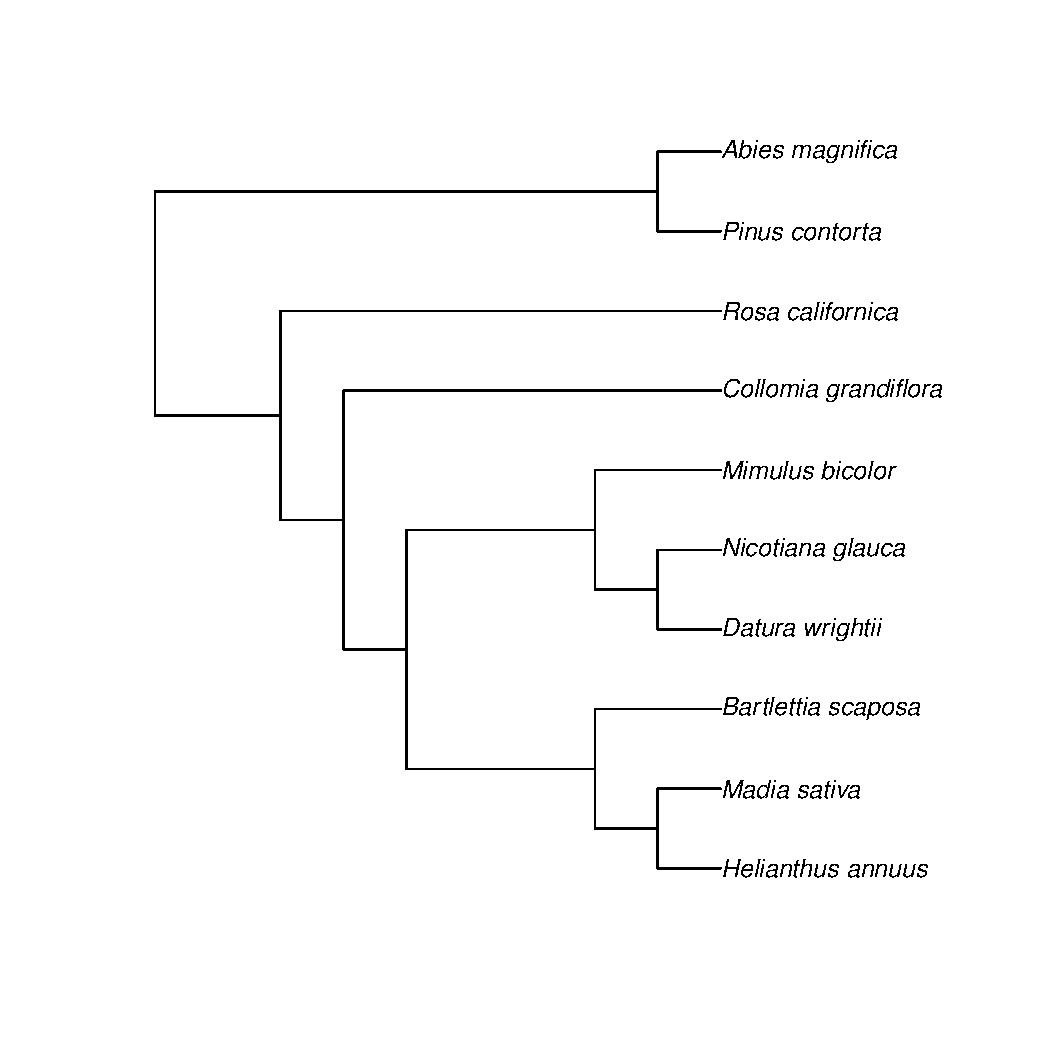
\includegraphics[width=4in,height=4in]{appendix/taxize/one/phylogeny.pdf} 

}

\caption[A phylogeny created using taxize]{A phylogeny created using taxize.\label{fig:phylophylogeny}}
\end{figure}
\end{knitrout}



Using the species list, with the corrected names, we can now search for occurrence data. The Global Biodiversity Information Facility (GBIF) has the largest collection of records data, and has a  API that we can interact with programmatically from R. First, we need to install rgbif.

\begin{knitrout}
\definecolor{shadecolor}{rgb}{0.969, 0.969, 0.969}\color{fgcolor}\begin{kframe}
\begin{alltt}
\hlcom{# Install rgbif from github.com}
\hlkwd{install.packages}\hlstd{(}\hlstr{"devtools"}\hlstd{)}
\hlkwd{library}\hlstd{(devtools)}
\hlkwd{install_github}\hlstd{(}\hlstr{"rgbif"}\hlstd{,} \hlstr{"ropensci"}\hlstd{)}
\end{alltt}
\end{kframe}
\end{knitrout}


Now we can search for occurrences for our species list and make a map.


\begin{knitrout}
\definecolor{shadecolor}{rgb}{0.969, 0.969, 0.969}\color{fgcolor}\begin{kframe}
\begin{alltt}
\hlkwd{library}\hlstd{(rgbif)}
\hlkwd{library}\hlstd{(ggplot2)}
\hlcom{# get occurences}
\hlstd{occurr_list} \hlkwb{<-} \hlkwd{occurrencelist_many}\hlstd{(}\hlkwd{as.character}\hlstd{(allnames}\hlopt{$}\hlstd{spname),} 
    \hlkwc{coordinatestatus} \hlstd{=} \hlnum{TRUE}\hlstd{,}
    \hlkwc{maxresults} \hlstd{=} \hlnum{100}\hlstd{,} \hlkwc{removeZeros} \hlstd{=} \hlnum{TRUE}\hlstd{,} 
    \hlkwc{fixnames} \hlstd{=} \hlstr{"changealltorig"}\hlstd{)}
\hlcom{# Make a map}
\hlstd{p} \hlkwb{<-} \hlkwd{gbifmap_list}\hlstd{(occurr_list)} \hlopt{+} 
    \hlkwd{guides}\hlstd{(}\hlkwc{col} \hlstd{=} \hlkwd{guide_legend}\hlstd{(}\hlkwc{title} \hlstd{=} \hlstr{""}\hlstd{,} \hlkwc{nrow} \hlstd{=} \hlnum{3}\hlstd{,}
    \hlkwc{byrow} \hlstd{=} \hlnum{TRUE}\hlstd{))} \hlopt{+} \hlkwd{theme}\hlstd{(}\hlkwc{legend.position} \hlstd{=} \hlstr{"bottom"}\hlstd{,} 
    \hlkwc{legend.key} \hlstd{=} \hlkwd{element_blank}\hlstd{())} \hlopt{+}
    \hlkwd{coord_equal}\hlstd{()}
\hlstd{p}
\end{alltt}
\end{kframe}\begin{figure}[h]


{\centering 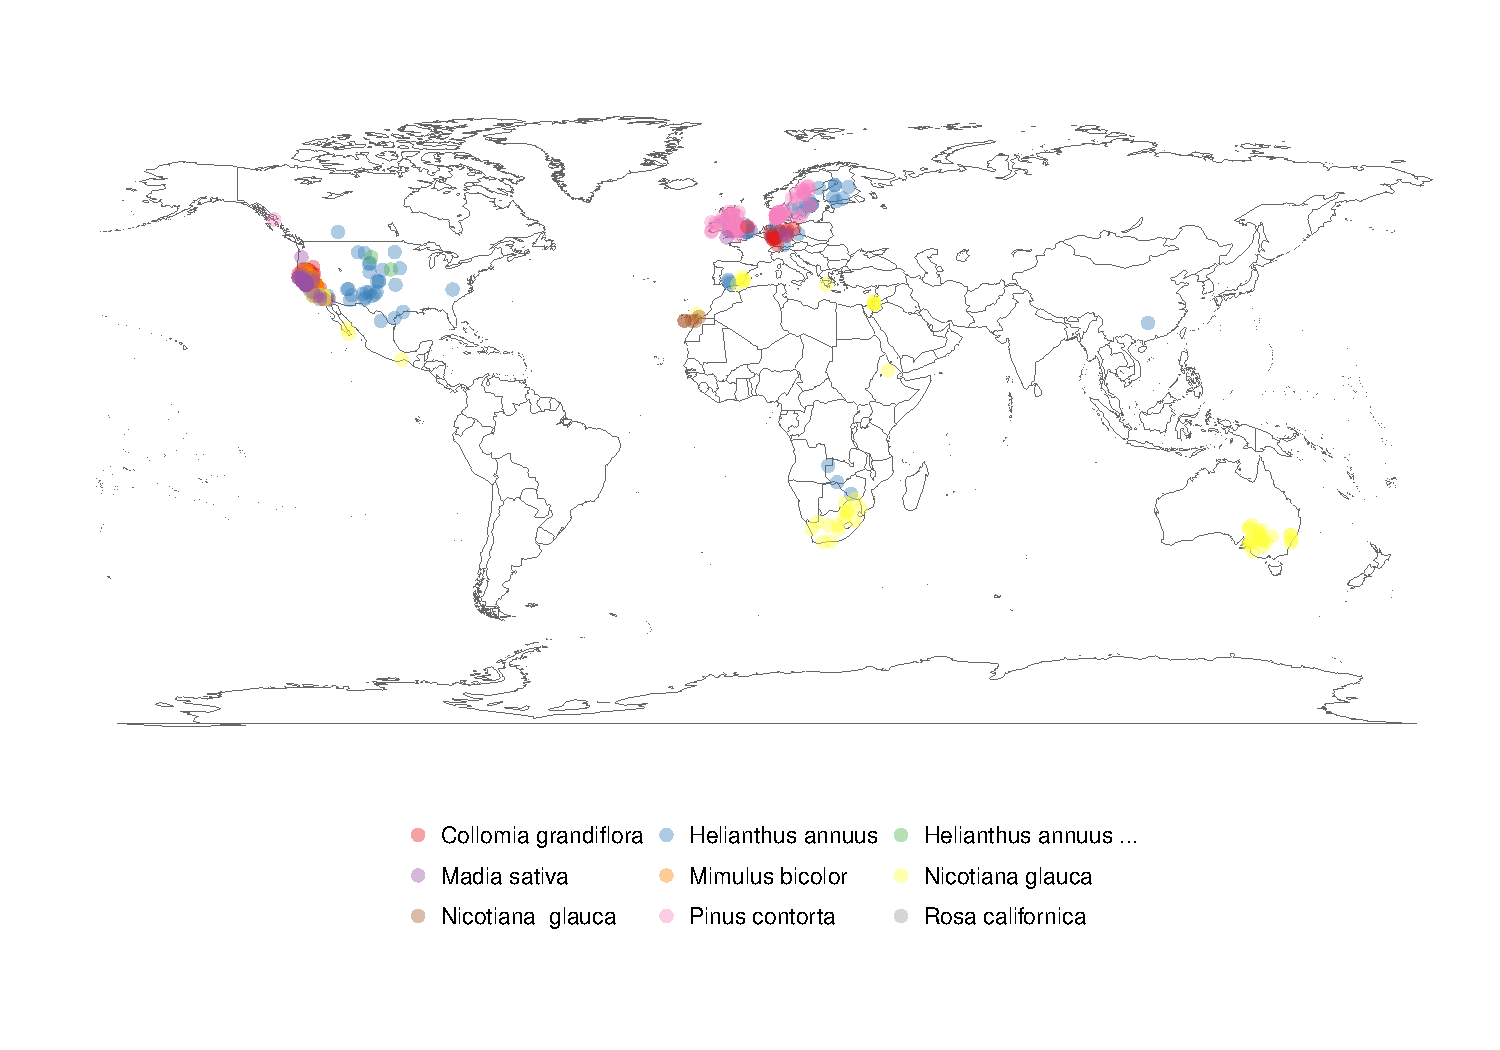
\includegraphics[width=0.9\textwidth]{appendix/taxize/one/plot_map.pdf} 

}

\caption[A map created using taxize]{A map created using taxize.\label{fig:mapplot_map}}
\end{figure}


\end{knitrout}

\end{document}
 

% -*- root: ../../../thesis.tex -*-

\section[Matching species tables]{Matching species tables with different taxonomic resolution} 
\label{ap:taxize:two} 

Trait-based approaches are a promising tool in ecology. Unlike taxonomy-based methods, traits may not be constrained to biogeographic boundaries \citep{baird_toward_2011} and have potential to disentangle the effects of multiple stressors \citep{statzner_can_2010}. 

To analyse trait-composition abundance data must be matched with trait data\-bases like \citep{usseglio-polatera_biological_2000}. However these two datatables may contain species information on different taxonomic levels and perhaps data must be aggregated to a joint taxonomic level.

taxize can help in this data-cleaning step, providing a reproducible workflow. Here we illustrate this on a small fictitious example.

Suppose we have fuzzy coded trait table with 2 traits with 3 respectively 2 modalities:

\begin{knitrout}
\color{fgcolor}\small\begin{kframe}
\begin{alltt}
\hlstd{(traits} \hlkwb{<-} \hlkwd{read.table}\hlstd{(}\hlkwc{header} \hlstd{=} \hlnum{TRUE}\hlstd{,} \hlkwc{sep} \hlstd{=} \hlstr{';'}\hlstd{,} \hlkwc{stringsAsFactors}\hlstd{=}\hlnum{FALSE}\hlstd{,}
                      \hlkwc{text} \hlstd{=} \hlstr{'taxon;T1M1;T1M2;T1M3;T2M1;T2M2
Gammarus sp.;0;0;3;1;3
Potamopyrgus antipodarum;1;0;3;1;3
Coenagrion sp.;3;0;1;3;1
Enallagma cyathigerum;0;3;1;0;3
Erythromma sp.;0;0;3;3;1
Baetis sp.;0;0;0;0;0
'}\hlstd{))}
\end{alltt}
\begin{verbatim}
                     taxon T1M1 T1M2 T1M3 T2M1 T2M2
1             Gammarus sp.    0    0    3    1    3
2 Potamopyrgus antipodarum    1    0    3    1    3
3           Coenagrion sp.    3    0    1    3    1
4    Enallagma cyathigerum    0    3    1    0    3
5           Erythromma sp.    0    0    3    3    1
6               Baetis sp.    0    0    0    0    0
\end{verbatim}
\end{kframe}
\end{knitrout}


And want to match this to a table with abundances:
\begin{knitrout}
\color{fgcolor}\small\begin{kframe}
\begin{alltt}
\hlstd{(abundances} \hlkwb{<-} \hlkwd{read.table}\hlstd{(}\hlkwc{header} \hlstd{=} \hlnum{TRUE}\hlstd{,} \hlkwc{sep} \hlstd{=} \hlstr{';'}\hlstd{,} \hlkwc{stringsAsFactors}\hlstd{=}\hlnum{FALSE}\hlstd{,}
                          \hlkwc{text} \hlstd{=} \hlstr{'taxon;abundance;sample
Gammarus roeseli;5;1
Gammarus roeseli;6;2
Gammarus tigrinus;7;1
Gammarus tigrinus;8;2
Coenagrionidae;10;1
Coenagrionidae;6;2
Potamopyrgus antipodarum;10;1
xxxxx;10;2
'}\hlstd{))}
\end{alltt}
\begin{verbatim}
                     taxon abundance sample
1         Gammarus roeseli         5      1
2         Gammarus roeseli         6      2
3        Gammarus tigrinus         7      1
4        Gammarus tigrinus         8      2
5           Coenagrionidae        10      1
6           Coenagrionidae         6      2
7 Potamopyrgus antipodarum        10      1
8                    xxxxx        10      2
\end{verbatim}
\end{kframe}
\end{knitrout}



First we do some basic data-cleaning and create a lookup-table, that will link taxa in trait table with the abundance table.
\begin{knitrout}
\color{fgcolor}\small\begin{kframe}
\begin{alltt}
\hlcom{# first we remove ' sp.' from out trait table:}
\hlstd{traits}\hlopt{$}\hlstd{taxon_cleaned} \hlkwb{<-} \hlkwd{tolower}\hlstd{(}\hlkwd{gsub}\hlstd{(}\hlstr{" sp."}\hlstd{,} \hlstr{""}\hlstd{, traits}\hlopt{$}\hlstd{taxon))}
\hlcom{# since abundance tables can be very long with repeating taxa, we look only}
\hlcom{# at unique taxon names This will be a lookup-table linking taxon names}
\hlcom{# between both tables}
\hlstd{lookup} \hlkwb{<-} \hlkwd{data.frame}\hlstd{(}\hlkwc{taxon} \hlstd{=} \hlkwd{tolower}\hlstd{(}\hlkwd{unique}\hlstd{(abundances}\hlopt{$}\hlstd{taxon)),} 
            \hlkwc{stringsAsFactors} \hlstd{=} \hlnum{FALSE}\hlstd{)}
\end{alltt}
\end{kframe}
\end{knitrout}


The we query the taxonomic hierarchy for both tables, this will be the backbone of this procedure:
\begin{knitrout}
\color{fgcolor}\small\begin{kframe}
\begin{alltt}
\hlkwd{library}\hlstd{(taxize)}
\hlstd{traits_classi} \hlkwb{<-} \hlkwd{classification}\hlstd{(}\hlkwd{get_uid}\hlstd{(traits}\hlopt{$}\hlstd{taxon_cleaned))}
\hlstd{lookup_classi} \hlkwb{<-} \hlkwd{classification}\hlstd{(}\hlkwd{get_uid}\hlstd{(lookup}\hlopt{$}\hlstd{taxon))}
\end{alltt}
\end{kframe}
\end{knitrout}


First we look if we can find any direct matches between taxon names:
\begin{knitrout}
\color{fgcolor}\small\begin{kframe}
\begin{alltt}
\hlcom{# first search for direct matches}
\hlstd{direct} \hlkwb{<-} \hlkwd{match}\hlstd{(lookup}\hlopt{$}\hlstd{taxon, traits}\hlopt{$}\hlstd{taxon_cleaned)}
\hlcom{# and add the matched name to our lookup table}
\hlstd{lookup}\hlopt{$}\hlstd{traits} \hlkwb{<-} \hlkwd{tolower}\hlstd{(traits}\hlopt{$}\hlstd{taxon[direct])}
\hlstd{lookup}\hlopt{$}\hlstd{match} \hlkwb{<-} \hlkwd{ifelse}\hlstd{(}\hlopt{!}\hlkwd{is.na}\hlstd{(direct),} \hlstr{"direct"}\hlstd{,} \hlnum{NA}\hlstd{)}
\hlstd{lookup}
\end{alltt}
\begin{verbatim}
                     taxon                   traits  match
1         gammarus roeseli                     <NA>   <NA>
2        gammarus tigrinus                     <NA>   <NA>
3           coenagrionidae                     <NA>   <NA>
4 potamopyrgus antipodarum potamopyrgus antipodarum direct
5                    xxxxx                     <NA>   <NA>
\end{verbatim}
\end{kframe}
\end{knitrout}


We found a direct match - \emph{potamopyrgus antipodarum} - so nothing to do here.


Next we look for species which are on a higher taxonomic resolution than our trait table. 
For these species we will take directly the trait-data since no better information is available.

\begin{knitrout}
\color{fgcolor}\small\begin{kframe}
\begin{alltt}
\hlcom{# look for cases where taxonomic resolution in abundance data is higher}
\hlcom{# than in trait data: here we take the trait-values for the lower}
\hlcom{# resolution}.
\hlkwa{for} \hlstd{(i} \hlkwa{in} \hlkwd{which}\hlstd{(}\hlkwd{is.na}\hlstd{(lookup}\hlopt{$}\hlstd{traits))) \{}
    \hlkwa{if} \hlstd{(}\hlkwd{is.data.frame}\hlstd{(lookup_classi[[i]])) \{}
        \hlstd{matches} \hlkwb{<-} \hlkwd{tolower}\hlstd{(lookup_classi[[i]]}\hlopt{$}\hlstd{ScientificName)} \hlopt 
        \hlstd{traits}\hlopt{$}\hlstd{taxon_cleaned}
        \hlkwa{if} \hlstd{(}\hlkwd{any}\hlstd{(matches)) \{}
            \hlstd{lookup}\hlopt{$}\hlstd{traits[i]} \hlkwb{<-} \hlkwd{tolower}
            \hlstd{(lookup_classi[[i]]}\hlopt{$}\hlstd{ScientificName[matches])}
            \hlstd{lookup}\hlopt{$}\hlstd{match[i]} \hlkwb{<-} \hlstd{lookup_classi[[i]]}\hlopt{$}\hlstd{Rank[matches]}
        \hlstd{\}}
    \hlstd{\}}
\hlstd{\}}
\hlstd{lookup}
\end{alltt}
\begin{verbatim}
                     taxon                   traits  match
1         gammarus roeseli                 gammarus  genus
2        gammarus tigrinus                 gammarus  genus
3           coenagrionidae                     <NA>   <NA>
4 potamopyrgus antipodarum potamopyrgus antipodarum direct
5                    xxxxx                     <NA>   <NA>
\end{verbatim}
\end{kframe}
\end{knitrout}


So our abundance data has two \emph{Gammarus} species, however trait data is only on genus level.


The next step is to search for species were we have to aggregate trait-data, since our abundance data is on a lower taxonomic level.
We are walking the taxonomic latter for the species in our trait-data upwards and search for matches with out abundance data. Since we'll have many taxa in the trait-data belonging to one taxon, we'll take the median modality scores as an approximation. Of course also other methods may be used here, e.g. weighting by genetic distance.


\begin{knitrout}
\color{fgcolor}\small\begin{kframe}
\begin{alltt}
\hlcom{# look for cases taxonomic resolution in abundance data is lower than in}
\hlcom{# trait data, here we need to aggregate the trait-values (eg. median value}
\hlcom{# for modality)}
\hlkwa{for} \hlstd{(i} \hlkwa{in} \hlkwd{which}\hlstd{(}\hlkwd{is.na}\hlstd{(lookup}\hlopt{$}\hlstd{traits))) \{}
    \hlcom{# find matches}
    \hlstd{agg} \hlkwb{<-} \hlkwd{sapply}\hlstd{(traits_classi,} \hlkwa{function}\hlstd{(}\hlkwc{x}\hlstd{)} \hlkwd{any}\hlstd{(}
    \hlkwd{tolower}\hlstd{(x}\hlopt{$}\hlstd{ScientificName)} \hlopt
        \hlstd{lookup}\hlopt{$}\hlstd{taxon[i]))}
    \hlkwa{if} \hlstd{(}\hlkwd{sum}\hlstd{(agg)} \hlopt{>} \hlnum{1}\hlstd{) \{}
        \hlcom{# add taxon as aggregate to trait-table}
        \hlstd{traits} \hlkwb{<-} \hlkwd{rbind}\hlstd{(traits,} \hlkwd{c}\hlstd{(}\hlkwd{paste0}\hlstd{(lookup}\hlopt{$}\hlstd{taxon[i],} \hlstr{"-aggregated"}\hlstd{),} 
        \hlkwd{apply}\hlstd{(traits[agg,}
            \hlnum{2}\hlopt{:}\hlnum{6}\hlstd{],} \hlnum{2}\hlstd{, median),} \hlkwd{paste0}\hlstd{(lookup}\hlopt{$}\hlstd{taxon[i],} \hlstr{"-aggregated"}\hlstd{)))}
        \hlcom{# fill lookup table}
        \hlstd{lookup}\hlopt{$}\hlstd{traits[i]} \hlkwb{<-} \hlkwd{paste0}\hlstd{(lookup}\hlopt{$}\hlstd{taxon[i],} \hlstr{"-aggregated"}\hlstd{)}
        \hlstd{lookup}\hlopt{$}\hlstd{match[i]} \hlkwb{<-} \hlstr{"aggregated"}
    \hlstd{\}}
\hlstd{\}}
\hlstd{lookup}
\end{alltt}
\begin{verbatim}
#                      taxon                    traits      match
# 1         gammarus roeseli                  gammarus      genus
# 2        gammarus tigrinus                  gammarus      genus
# 3           coenagrionidae coenagrionidae-aggregated aggregated
# 4 potamopyrgus antipodarum  potamopyrgus antipodarum     direct
# 5                    xxxxx                      <NA>       <NA>
\end{verbatim}
\end{kframe}
\end{knitrout}


Finally we have only one taxon left - clearly an error. We remove this from our dataset:
\begin{knitrout}
\color{fgcolor}\small\begin{kframe}
\begin{alltt}
\hlstd{abundances} \hlkwb{<-} \hlstd{abundances[}\hlopt{!}\hlstd{abundances}\hlopt{$}\hlstd{taxon} \hlopt{==} \hlstd{lookup}\hlopt{$}\hlstd{taxon[}\hlkwd{is.na}\hlstd{(}
                        \hlstd{lookup}\hlopt{$}\hlstd{traits)],}
    \hlstd{]}
\end{alltt}
\end{kframe}
\end{knitrout}



Now we can create \emph{species x sites} and \emph{traits x species} matrices, which could be plugged into methods to analyse trait responses [28].


\begin{knitrout}
\color{fgcolor}\small\begin{kframe}
\begin{alltt}
\hlcom{# species (as matched with trait table) by site matrix}
\hlstd{abundances}\hlopt{$}\hlstd{traits_taxa} \hlkwb{<-} \hlstd{lookup}\hlopt{$}\hlstd{traits[}\hlkwd{match}\hlstd{(}\hlkwd{tolower}\hlstd{(abundances}\hlopt{$}\hlstd{taxon), 
                lookup}\hlopt{$}\hlstd{taxon)]}
\hlkwd{library}\hlstd{(reshape2)}
\hlcom{# reshape data to long format and name rows by samples}
\hlstd{L} \hlkwb{<-} \hlkwd{dcast}\hlstd{(abundances, sample} \hlopt{~} \hlstd{traits_taxa,} \hlkwc{fun.aggregate} \hlstd{= sum,} 
          \hlkwc{value.var} \hlstd{=} \hlstr{"abundance"}\hlstd{)}
\hlkwd{rownames}\hlstd{(L)} \hlkwb{<-} \hlstd{L}\hlopt{$}\hlstd{sample}
\hlstd{L}\hlopt{$}\hlstd{sample} \hlkwb{<-} \hlkwa{NULL}
\hlstd{L}
\end{alltt}
\begin{verbatim}
#   coenagrionidae-aggregated gammarus potamopyrgus antipodarum
# 1                        10       12                       10
# 2                         6       14                        0
\end{verbatim}
\begin{alltt}
\hlcom{# traits by species matrix}
\hlstd{Q} \hlkwb{<-} \hlstd{traits[,} \hlnum{2}\hlopt{:}\hlnum{7}\hlstd{][}\hlkwd{match}\hlstd{(}\hlkwd{names}\hlstd{(L), traits}\hlopt{$}\hlstd{taxon_cleaned), ]}
\hlkwd{rownames}\hlstd{(Q)} \hlkwb{<-} \hlstd{Q}\hlopt{$}\hlstd{taxon_cleaned}
\hlstd{Q}\hlopt{$}\hlstd{taxon_cleaned} \hlkwb{<-} \hlkwa{NULL}
\hlstd{Q}
\end{alltt}
\begin{verbatim}
#                           T1M1 T1M2 T1M3 T2M1 T2M2
# coenagrionidae-aggregated    0    0    1    3    1
# gammarus                     0    0    3    1    3
# potamopyrgus antipodarum     1    0    3    1    3
\end{verbatim}
\begin{alltt}
\hlcom{# check}
\hlkwd{all}\hlstd{(}\hlkwd{rownames}\hlstd{(Q)} \hlopt{==} \hlkwd{colnames}\hlstd{(L))}
\end{alltt}
\begin{verbatim}
# [1] TRUE
\end{verbatim}
\end{kframe}
\end{knitrout}


This is just an example how taxonomic APIs (via taxize) could be used to search for matches up- and downwards the taxonomic ladder. We are looking forward to integrate other databases into taxize, which will facilitate trait-based analyses in R.


%% ----------------------------------------------------------------------------
\clearpage
\section{References}
\printbibliography[heading=none]






%----------------------------------------------------------------------------
\backmatter

%----------------------------------------------------------------------------
% Authors contributions
\cleardoublepage
\def\dir{frontbackmatter}
\setstretch{1}
% -*- root: ../thesis.tex -*-


\chapter{Author's contributions}

% \thispagestyle{empty}
% \begingroup
% \let\clearpage\relax
% \let\cleardoublepage\relax
% \let\cleardoublepage\relax
% \thispagestyle{empty}


\begin{sloppypar}

\section*{Article I}
\vspace{-1em}
\small
\begin{description}
    \setlength\itemsep{0em}
	\item[Title:] Ecotoxicology is not normal - A comparison of statistical approaches for analysis of count and proportion data in ecotoxicology
	\item[Authors:] \textbf{Eduard Szöcs} and Ralf B. Schäfer
	\item[Status:] Published in 2015 in Environmental Science and Pollution Research, Volume 22, Issue 18, pp 13990-13999
	\item[Contributions:] \textbf{Szöcs} (85\%) Designed research and simulations, analysed data, discussed results, wrote manuscript 

	Schäfer (15\%) Designed research, discussed results, edited manuscript
\end{description}
\normalsize
\vfill

\section*{Article II}
\vspace{-1em}
\small
\begin{description}
    \setlength\itemsep{0em}
	\item[Title:] Large scale risks from pesticides in small streams
	\item[Authors:] \textbf{Eduard Szöcs}, Marvin Brinke, Bilgin Karaoglan, and Ralf B. Schäfer
	\item[Status:] Submitted to \emph{Environmental Science \& Technology} in 2016
	\item[Contributions:] \textbf{Szöcs} (75\%) Designed research, analysed data, discussed results, wrote manuscript

	Brinke (5\%) helped with data, commented on manuscript

	Karaoglan (5\%) provided data (RACs), commented on manuscript

	Schäfer (15\%) Designed research, discussed results, edited manuscript
\end{description}
\normalsize
\vfill

\section*{Article III}
\vspace{-1em}
\small
\begin{description}
    \setlength\itemsep{0em}
	\item[Title:] webchem: An R Package to Retrieve Chemical Information from the Web.
	\item[Authors:] \textbf{Eduard Szöcs} and Ralf B. Schäfer
	\item[Status:] Accepted in 2016 in \emph{Journal of Statistical Software}
	\item[Contributions:] \textbf{Szöcs} (90\%) Designed, programmed and tested software, wrote manuscript

	Schäfer (10\%) discussed results, edited manuscript
\end{description}
\normalsize
\vfill


\section*{Article IV}
\vspace{-1em}
\small
\begin{description}
    \setlength\itemsep{0em}
	\item[Title:] taxize: taxonomic search and retrieval in R
	\item[Authors:] Scott A. Chamberlain and \textbf{Eduard Szöcs}
	\item[Status:] Published in 2013 in \emph{F1000Research, Volume 2, Issue 191}
	\item[Contributions:] Chamberlain (50\%) Designed, programmed and tested software, wrote manuscript

	\textbf{Szöcs} (50\%) Designed, programmed and tested software, wrote manuscript
\end{description}
\end{sloppypar}


% \endgroup

\setstretch{1.12}


%----------------------------------------------------------------------------
% Declaration
\cleardoublepage
\def\dir{frontbackmatter}
\chapter{Declaration}

I, the author of this work, certify that this work contains no material which has been accepted or submitted for the award of any other degree at any university or other tertiary institution.
The work has been interdependently prepared. 
All aids and sources have been clearly specified and the contribution of other authors have been documented and reference lists given.



\signature{Eduard Szöcs}



%----------------------------------------------------------------------------
% CV
\cleardoublepage
\def\dir{frontbackmatter}
% -*- root: ../thesis.tex -*-

\newgeometry{top = 100mm}

\addcontentsline{toc}{chapter}{\textsc{curriculum vitae}}

% adapt included pdf to layout size
% http://tex.stackexchange.com/questions/46888/pdfpages-package-and-layoutsize-geometry-package
\iftoggle{print}{%
	\includepdf[pages=-, scale=.95,
    offset=0mm 25mm
		]{frontbackmatter/cv/escv.pdf}
}{
	\includepdf[pages=-, scale=.95
		]{frontbackmatter/cv/escv.pdf}
}



\restoregeometry
\thispagestyle{empty}


%----------------------------------------------------------------------------
% Colophon
% should be on left page (=last page)
\cleartoleftpage
\def\dir{frontbackmatter}
% -*- root: ../thesis.tex -*-

\pagestyle{empty}

\hfill

\vfill


\pdfbookmark[0]{Colophon}{colophon}
\section*{Colophon}
This document was typeset in \LaTeX~using a slightly customized version of the 
\texttt{classicthesis} typography by Prof. Miede (\url{http://www.miede.de/}). Most of the graphics in this thesis are generated using \texttt{pgf/tikz}.
The bibliography is typeset using \texttt{biblatex}.
This thesis and the source code is also available from \url{https://github.com/EDiLD/phd_thesis}.




\end{document}
 
